% ===========================================================================
%  Three-Phase Two-Level SiC Traction Inverter
%  Project 7 - Automotive Power Electronics Circuit Design
%  Universita' di Bologna
%
%  Compilazione:  latexmk -pdf main.tex        (oppure make)
%  Le figure vanno sincronizzate prima con:    python aggiorna_figure.py
% ===========================================================================
\documentclass[11pt,a4paper,twoside,openright]{report}

% ---------------------------------------------------------------------------
%  Preambolo comune. Tenuto separato da main.tex cosi' che l'indice dei
%  capitoli resti leggibile in un colpo d'occhio.
% ---------------------------------------------------------------------------

% --- lingua e codifica -----------------------------------------------------
\usepackage[T1]{fontenc}
\usepackage[utf8]{inputenc}
\usepackage[english]{babel}
\usepackage{lmodern}
\usepackage{microtype}

% --- impaginazione ---------------------------------------------------------
\usepackage[a4paper,inner=3cm,outer=2.5cm,top=2.8cm,bottom=2.8cm]{geometry}
\usepackage{fancyhdr}
\usepackage{emptypage}
\setlength{\parskip}{0.4em}

\setlength{\headheight}{14pt}   % richiesto da fancyhdr
\pagestyle{fancy}
\fancyhf{}
\fancyhead[LE,RO]{\thepage}
\fancyhead[RE]{\nouppercase{\leftmark}}
\fancyhead[LO]{\nouppercase{\rightmark}}
\renewcommand{\headrulewidth}{0.4pt}
\fancypagestyle{plain}{\fancyhf{}\fancyfoot[C]{\thepage}%
  \renewcommand{\headrulewidth}{0pt}}

% --- matematica ------------------------------------------------------------
\usepackage{amsmath}
\usepackage{amssymb}

% --- unita' di misura ------------------------------------------------------
% Un solo punto di configurazione per tutte le unita' del report: cosi' non
% si finisce con "30 A_RMS", "30 Arms" e "30 A rms" in tre capitoli diversi.
%
% NOTA SULLA SCELTA. Lo strumento naturale sarebbe siunitx, ed e' quello per
% cui la sintassi qui sotto e' scritta. Su questa macchina non e' usabile:
% MiKTeX ha siunitx 3.5.12 (2026-09-08) su un kernel LaTeX2e 2023-11-01 con
% L3 2024-01-04, e il pacchetto usa variabili che quel kernel non definisce.
% Fallisce anche su un documento minimo di quattro righe, quindi non e' un
% problema di questo report.
%
% Per non lasciare il documento ostaggio di un toolchain rotto, le macro
% sono reimplementate qui in LaTeX puro. I punti di chiamata restano
% identici a siunitx: quando MiKTeX sara' aggiornato bastera' cancellare
% questo blocco e togliere il commento alle due righe in fondo.
\usepackage{textcomp}

\makeatletter
% I simboli sono definiti GLOBALMENTE, non solo dentro \si. Serve perche'
% \caption scrive i propri argomenti negli elenchi di figure e tabelle cosi'
% come sono: la' dentro \volt viene riletto a livello superiore, e se fosse
% definito solo localmente sarebbe una sequenza non definita.
% prefissi
\def\yocto{y}\def\pico{p}\def\nano{n}\def\micro{\textmu}\def\milli{m}
\def\centi{c}\def\deci{d}\def\kilo{k}\def\mega{M}\def\giga{G}
% unita' di base e derivate usate nel report
\def\metre{m}\def\meter{m}\def\second{s}\def\gram{g}\def\kelvin{K}\def\minute{min}
\def\ampere{A}\def\volt{V}\def\watt{W}\def\joule{J}\def\hertz{Hz}
% L'ohm NON usa \textohm: il glifo TS1 ha una mappatura ToUnicode rotta e
% l'estrazione di testo dal PDF restituisce "W" al posto di "ohm", rendendo
% inutilizzabili ricerca e copia-incolla ("40 mohm" diventava "40 mW").
% L'Omega matematico e' dritto per default in TeX ed e' mappato bene.
\def\ohm{\ensuremath{\Omega}}\def\farad{F}\def\henry{H}\def\coulomb{C}
\def\siemens{S}\def\celsius{\textcelsius}\def\percent{\%}
\def\VA{VA}\def\var{var}
\def\degree{\textdegree}\def\rpm{rpm}
% raffreddamento (11/10/2026): portate, pressioni, volumi. Litro maiuscolo:
% la l minuscola accanto a un numero si legge 1 ("10 l/min" sembrava "101/min")
\def\litre{L}\def\liter{L}\def\pascal{Pa}\def\hour{h}\def\decibel{dB}\def\cubic#1{#1\ensuremath{^{3}}}
% grandezze efficaci e di picco: scritte sempre allo stesso modo
\def\Arms{A\textsubscript{rms}}\def\Vrms{V\textsubscript{rms}}
\def\Apk{A\textsubscript{pk}}\def\Vpk{V\textsubscript{pk}}
% separatore
\def\per{/}
\def\squared{\ensuremath{^{2}}}\def\cubed{\ensuremath{^{3}}}
\let\pecd@units\relax

% Tutte protette: compaiono dentro \caption, che scrive negli elenchi di
% figure e tabelle. Senza \protected verrebbero espanse durante quella
% scrittura, dove i simboli di \pecd@units non sono definiti.
% Numero: \ensuremath cosi' che \pm, \times e simili funzionino.
\protected\def\num#1{\ensuremath{#1}}
% Unita' sola.
\protected\def\si#1{{\pecd@units\textup{#1}}}
% Parte unita' di \SI: se vuota non mette lo spazio fine, cosi' si possono
% scrivere intervalli come \SI{10}{}--\SI{30}{\kilo\hertz}.
\protected\def\pecd@unit#1{%
  \edef\pecd@tmp{\detokenize{#1}}%
  \ifx\pecd@tmp\@empty\else\,\si{#1}\fi}
\protected\def\SI#1#2{\num{#1}\pecd@unit{#2}}
\protected\def\qty#1#2{\SI{#1}{#2}}
\protected\def\numrange#1#2{\num{#1}\,--\,\num{#2}}
\protected\def\SIrange#1#2#3{\num{#1}\,--\,\SI{#2}{#3}}
% Accettate e ignorate, per compatibilita' con la sintassi siunitx.
\newcommand{\sisetup}[1]{}
\newcommand{\DeclareSIUnit}[2]{}
\makeatother

% Quando MiKTeX sara' aggiornato, sostituire tutto il blocco qui sopra con:
%   \usepackage{siunitx}
%   \sisetup{detect-all, per-mode=symbol}
%   \DeclareSIUnit{\Arms}{A_{\mathrm{rms}}}  ... e le altre tre

% --- figure e tabelle ------------------------------------------------------
\usepackage{graphicx}
\graphicspath{{figures/}}
\usepackage{booktabs}
\usepackage{tabularx}
\usepackage{multirow}
\usepackage{longtable}
\usepackage[font=small,labelfont=bf]{caption}
\usepackage{subcaption}
\usepackage{float}
\usepackage{rotating}   % sidewaysfigure: fogli dello schema in orizzontale (cap. 9)

% Pagine di soli float: in alto e a distanza fissa. Di default LaTeX le
% centra in verticale e lascia mezzi fogli bianchi fra una tabella e una figura.
\makeatletter
\setlength{\@fptop}{0pt}
\setlength{\@fpsep}{2\baselineskip}
\setlength{\@fpbot}{0pt plus 1fil}
\makeatother

% colonna centrata a larghezza automatica per le tabelle numeriche
% Colonne di testo allineate a sinistra: una cella su piu' righe centrata si
% legge male (revisione dell'11/10/2026).
\newcolumntype{Y}{>{\raggedright\arraybackslash}X}
\newcolumntype{L}[1]{>{\raggedright\arraybackslash}p{#1}}

% --- colori e riquadri -----------------------------------------------------
\usepackage[table]{xcolor}
\definecolor{notebg}{RGB}{245,245,245}
\definecolor{noteline}{RGB}{120,120,120}
\usepackage[most]{tcolorbox}

% Riquadro per le discrepanze trovate durante il lavoro. Sono il valore
% aggiunto del progetto rispetto a un'esecuzione a ricetta, quindi hanno un
% formato riconoscibile invece di sparire nel corpo del testo.
\newtcolorbox{finding}[1]{%
  colback=notebg, colframe=noteline, boxrule=0.4pt, arc=1pt,
  left=6pt, right=6pt, top=5pt, bottom=5pt,
  title={\textbf{#1}}, fonttitle=\small, coltitle=black,
  colbacktitle=notebg, breakable}

% --- codice ----------------------------------------------------------------
% Schemi disegnati (figures/tikz/): TikZ e' gia' caricato da tcolorbox.
% Palette uguale a quella delle figure Python (config.COLORI): leggibile in
% scala di grigi e dai daltonici.
\usepackage[european,straightvoltages]{circuitikz}
\usepackage{pgfplots}
\pgfplotsset{compat=1.17}
\usetikzlibrary{arrows.meta,positioning,calc,fit,backgrounds,decorations.pathreplacing,shapes.geometric,shapes.misc}
\definecolor{fblu}{HTML}{0072B2}
\definecolor{farancio}{HTML}{D55E00}
\definecolor{fverde}{HTML}{009E73}
\definecolor{fgrigio}{HTML}{777777}

% --- tabelle leggibili (revisione del 18/10/2026) --------------------------
% \zebra prima di un tabular: righe alterne grigio chiaro (colortbl, possibile
% dopo l'aggiornamento di MiKTeX del 18/10/2026), un po' piu' di aria fra le
% righe. Le celle PASS/FAIL hanno lo sfondo dell'esito.
\newcommand{\zebra}{\rowcolors{2}{white}{black!6}\renewcommand{\arraystretch}{1.15}}
\newcommand{\pass}[1]{\cellcolor{fverde!30}#1}
\newcommand{\fail}[1]{\cellcolor{farancio!30}#1}
\newcommand{\aperto}[1]{\cellcolor{yellow!45}#1}
\newcommand{\nd}{\cellcolor{black!10}--}
\usepackage{listings}
\lstset{
  basicstyle=\ttfamily\footnotesize,
  breaklines=true,
  frame=single,
  rulecolor=\color{noteline},
  columns=fullflexible,
  keepspaces=true
}

% --- bibliografia ----------------------------------------------------------
\usepackage{csquotes}   % richiesto da biblatex quando c'e' babel
\usepackage[backend=biber,style=ieee,sorting=none]{biblatex}
\addbibresource{references.bib}

% --- riferimenti incrociati ------------------------------------------------
\usepackage[hidelinks]{hyperref}
\hypersetup{
  pdftitle  = {Three-Phase Two-Level SiC Traction Inverter},
  pdfauthor = {Matteo Borghi},
  pdfsubject= {Automotive Power Electronics Circuit Design, Project 7},
  bookmarksnumbered = true
}
\usepackage[capitalise,noabbrev]{cleveref}
\crefname{chapter}{Chapter}{Chapters}
\crefname{section}{Section}{Sections}
\crefname{figure}{Figure}{Figures}
\crefname{table}{Table}{Tables}
\crefname{equation}{Equation}{Equations}
% dopo \appendix i capitoli sono appendici: "Appendix A", non "Chapter A"
\crefname{appendix}{Appendix}{Appendices}

% --- macro di progetto -----------------------------------------------------
% I nomi ricorrenti si scrivono una volta sola: se cambia il dispositivo,
% cambia qui e non in trenta punti del testo.
\newcommand{\device}{E3M0016120K}
\newcommand{\driver}{UCC21750}
\newcommand{\isoamp}{AMC1302}
\newcommand{\isoampv}{AMC1311}
\newcommand{\dcdc}{MGJ2D121505SC}
\newcommand{\Rthjc}{R_{\theta,\mathrm{JC}}}
\newcommand{\Rthcs}{R_{\theta,\mathrm{CS}}}
\newcommand{\Rthha}{R_{\theta,\mathrm{HA}}}
\newcommand{\Tj}{T_{\mathrm{j}}}
\newcommand{\Tcase}{T_{\mathrm{case}}}
\newcommand{\Ths}{T_{\mathrm{hs}}}
\newcommand{\Rdson}{R_{\mathrm{DS(on)}}}
\newcommand{\Eon}{E_{\mathrm{on}}}
\newcommand{\Eoff}{E_{\mathrm{off}}}
\newcommand{\fsw}{f_{\mathrm{sw}}}
\newcommand{\Vdc}{V_{\mathrm{DC}}}

% Segnaposto visibile per i capitoli non ancora scrivibili.
\newcommand{\stubnote}[1]{%
  \begin{center}
  \fcolorbox{noteline}{notebg}{%
    \parbox{0.9\textwidth}{\small\textbf{Placeholder.} #1}}
  \end{center}}


\begin{document}

% --------------------------------------------------------------- frontespizio
\begin{titlepage}
\centering
\vspace*{2cm}

{\Large\scshape University of Bologna}\\[0.3cm]
{\large School of Engineering}\\[2.5cm]

{\large Automotive Power Electronics Circuit Design}\\[0.4cm]
{\large\bfseries Project 7}\\[1.5cm]

\rule{\textwidth}{0.5pt}\\[0.6cm]
{\huge\bfseries Design of a Three-Phase Two-Level\\[0.2cm]
SiC Traction Inverter\\[0.4cm]}
{\large \SI{800}{\volt} DC-link, \SI{30}{\Arms} per phase, \SI{20}{\kilo\hertz}}\\[0.5cm]
\rule{\textwidth}{0.5pt}\\[2.5cm]

{\large Matteo Borghi}\\[2cm]

{\large Academic Year 2025/2026}

\vfill
\end{titlepage}

\cleardoublepage
\pagenumbering{roman}

\chapter*{Abstract}
\addcontentsline{toc}{chapter}{Abstract}
This report documents the design of the power stage of a three-phase
two-level voltage-source inverter for an automotive traction application:
\SI{800}{\volt} on the DC-link, \SI{30}{\Arms} per phase at any load power
factor, \SI{20}{\kilo\hertz} switching frequency, and forced-air or liquid
cooling with a maximum ambient of \SI{50}{\celsius}. The device is the
Wolfspeed \device{} silicon-carbide MOSFET~\cite{wolfspeed_e3m0016}, selected
against seven alternatives (other device classes, a paralleled pair, a
top-side-cooled package and a module) on criteria fixed before any result was
computed.

The work covers the design equations (operating point, DC-link capacitor,
modulation, dead time), a circuit-level PLECS model validated against
closed-form results, a SPICE study of the switching cell that fixes the gate
resistances, the loss and thermal budget, and the schematic and layout of the
power stage as a module of a larger board.

At the design point the converter delivers \SI{25.48}{\kilo\watt} of active
power and dissipates \SI{128.1}{\watt}, an efficiency of \SI{99.50}{\percent},
with a current ripple of \SI{0.84}{\percent} in RMS terms. The DC-link of
\SI{200}{\micro\farad} keeps the voltage ripple at \SI{0.17}{\percent} at the
rated point and at \SI{0.36}{\percent} in the worst operating condition,
against \SI{0.5}{\percent}. The junction settles at \SI{81.8}{\celsius}. The
design is sized by the stalled motor, a case this design adds to the brief:
with the full \SI{42.4}{\ampere} peak flowing as direct current through one
device, the junction reaches \SI{111.1}{\celsius} on an ideal cold plate
against a \SI{120}{\celsius} design criterion. On a real liquid-cooled rail,
computed in three dimensions, the criterion is met only after the insulating
interface is redesigned: with aluminium nitride and a phase-change material
the hottest junction reaches \SI{97.9}{\celsius}, and \SI{117.8}{\celsius}
with every tolerance stacked.

Four findings would each have produced a wrong report had they gone
unnoticed. The device first used was industrial rather than automotive and,
at locked rotor, twenty degrees beyond the criterion; the selection that
replaced it was decided by overvoltage at the die, not by temperature. The
first double-pulse bench measured a DC bus that was still charging, which hid
nearly \SI{70}{\volt} of overshoot; with the real bus the turn-off gate
resistance had to rise from \SI{5}{} to \SI{12.5}{\ohm}, and switching became
more than half of the loss budget. The vendor loss tables refer to the
body-diode free-wheeling case, while the library folder name suggests the
external-diode case: a factor of 2.0 on the turn-on energy. And the largest
thermal unknown is the insulating pad between the case and the cold plate,
more precisely its two interfaces, which on the real rail decide more of the
junction temperature than the coolant does.


\cleardoublepage
\tableofcontents
\cleardoublepage
\listoffigures
\cleardoublepage
\listoftables

\cleardoublepage
\pagenumbering{arabic}

% ------------------------------------------------------------------ capitoli
\chapter{Introduction}
\label{ch:intro}

\section{Context and objective}

Traction inverters are the point where the electrical and the mechanical
domains of an electric vehicle meet, and they are the component in which the
move from silicon to wide-bandgap devices has had the clearest effect. Raising
the DC-link from the \SI{400}{\volt} class to the \SI{800}{\volt} class halves
the current for a given power, which reduces conduction losses and cable
cross-section, but it also puts the switching devices in a voltage class where
silicon IGBTs become slow and lossy. Silicon carbide MOSFETs are the natural
answer, and they bring their own set of problems: fast edges, small gate-drive
margins, and a body diode whose reverse recovery is not negligible.

The object of this work is the power stage of such a converter: the bridge,
the DC-link and the cooling, with the schematic and the board layout of that
module. \Cref{fig:system} shows what the module contains and where it stops:
the battery, the gate drive and the controller are outside it, and what
crosses its boundary is written down as an assumption (\cref{tab:sysassume}).
The report follows the four things the brief asks of it: the design
equations (\cref{ch:analytical,ch:modulation}), the component selection
(\cref{ch:spec}), the design choices, and the discussion of the numerical
simulations (\cref{ch:model,ch:losses,ch:thermal}). Every component value is
either taken from a datasheet, computed from a formula shown in the text, or
obtained from a simulation whose model is documented and validated.

\begin{figure}[htbp]
\centering
% Il power stage e i suoi confini: cosa sta dentro il modulo e cosa gli arriva da fuori.
\begin{tikzpicture}[
  font=\footnotesize, >=Stealth,
  blk/.style={draw, rounded corners=2pt, align=center, minimum height=10mm, inner sep=3pt, fill=white},
  hv/.style={blk, draw=farancio, fill=farancio!7},
  ext/.style={blk, dashed, draw=fgrigio},
  pw/.style={->, very thick, farancio}]
  % catena di potenza
  \node[ext, text width=17mm] (bat) at (0,0) {HV battery\\\SI{800}{\volt}};
  \node[hv, text width=26mm] (dcl) at (4.0,0) {DC-link\\film and ceramics};
  \node[hv, text width=38mm] (brg) at (8.6,0) {three-phase bridge\\$6\times$ SiC MOSFET, shunts};
  \node[draw, circle, minimum size=11mm] (mot) at (13.0,0) {M};
  \draw[pw] (bat) -- node[above, font=\scriptsize]{DC} (dcl);
  \draw[pw] (dcl) -- (brg);
  \draw[pw] (brg) -- node[above, font=\scriptsize]{3 phases} (mot);
  % raffreddamento: dentro il modulo, con il suo liquido fuori
  \node[hv, text width=38mm] (rail) at (8.6,1.9) {cooling rail, pad\\{\scriptsize liquid at \SI{65}{\celsius}}};
  \draw[->, thick, fgrigio] (brg) -- node[right, font=\scriptsize]{heat} (rail);
  % cio' che arriva da fuori
  \node[ext, text width=46mm] (ctl) at (8.6,-2.1) {gate drive, protection, controller\\{\scriptsize outside the module}};
  \draw[->, thick] (ctl.north) -- node[right, font=\scriptsize, pos=0.28]{gate and Kelvin-source signals} (brg.south);
  % confine del modulo
  \begin{scope}[on background layer]
    \node[draw=black, dash dot, rounded corners=4pt, inner sep=3mm,
          fit=(dcl)(brg)(rail)] (mod) {};
  \end{scope}
  \node[anchor=north west, font=\scriptsize\bfseries] at (mod.north west) {power stage module};
\end{tikzpicture}

\caption{The power stage and its boundaries. Orange: inside the module; dashed
grey: outside it, with the interface stated as assumptions
(\cref{tab:sysassume}).}
\label{fig:system}
\end{figure}

\section{Method and structure}

The design proceeds in four stages, each validating the previous one
(\cref{fig:flow}). Analytical sizing fixes the operating point, the DC-link
capacitance, the device rating and the modulation from closed-form relations
(\cref{ch:analytical,ch:modulation}). Circuit simulation builds a PLECS model
of the converter and uses it to obtain the losses; its outputs are reconciled
with the analytical results, the vendor loss tables it relies on are verified
against the datasheet, and a SPICE study of a single switching cell fixes the
gate resistances on the overvoltage at the die (\cref{ch:model,ch:losses}).
Thermal analysis closes the loop between losses and temperature, which this
device needs because its on-resistance rises by \SI{80}{\percent} between
\SI{25}{\celsius} and \SI{175}{\celsius}, and verifies the stalled-motor case
that selected the device (\cref{ch:thermal}). Schematic and layout turn the
design into a KiCad module (\cref{ch:schematic,ch:layout}).
\Cref{ch:conclusions} draws the conclusions and \cref{app:assumptions}
collects the assumptions that still need confirmation.

\begin{figure}[htbp]
\centering
% Il metodo: le fasi in avanti e i ritorni che hanno cambiato il progetto.
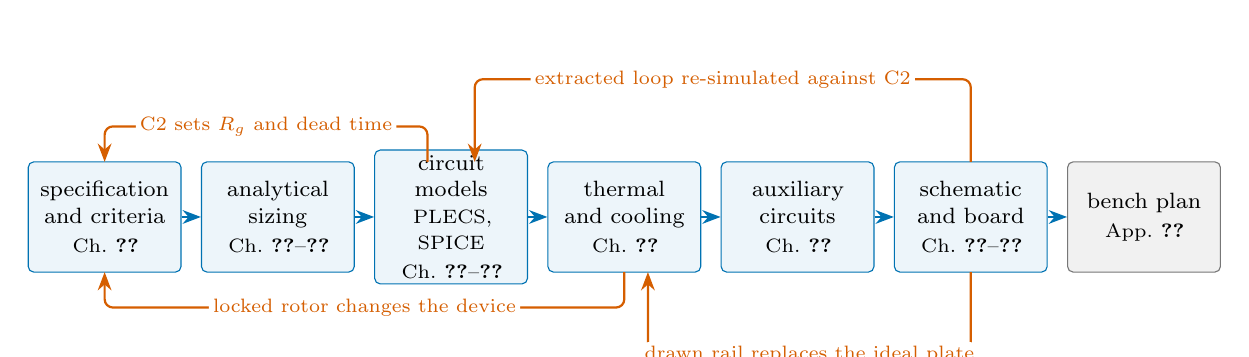
\begin{tikzpicture}[
  font=\footnotesize, >=Stealth,
  fase/.style={draw=fblu, fill=fblu!7, rounded corners=2pt, align=center, text width=18mm,
               minimum height=14mm, inner sep=2pt},
  ritorno/.style={->, farancio, thick, rounded corners=3pt},
  lab/.style={font=\scriptsize, farancio, fill=white, inner sep=1.5pt}]
  \node[fase] (s) at (0,0)     {specification\\and criteria\\[1pt]\scriptsize Ch.~\ref{ch:spec}};
  \node[fase] (a) at (2.2,0)   {analytical\\sizing\\[1pt]\scriptsize Ch.~\ref{ch:analytical}--\ref{ch:modulation}};
  \node[fase] (m) at (4.4,0)   {circuit models\\{\scriptsize PLECS, SPICE}\\[1pt]\scriptsize Ch.~\ref{ch:model}--\ref{ch:losses}};
  \node[fase] (t) at (6.6,0)   {thermal\\and cooling\\[1pt]\scriptsize Ch.~\ref{ch:thermal}};
  \node[fase] (x) at (8.8,0)   {auxiliary\\circuits\\[1pt]\scriptsize Ch.~\ref{ch:aux}};
  \node[fase] (b) at (11.0,0)  {schematic\\and board\\[1pt]\scriptsize Ch.~\ref{ch:schematic}--\ref{ch:layout}};
  \node[fase, draw=fgrigio, fill=fgrigio!10] (v) at (13.2,0) {bench plan\\[1pt]\scriptsize App.~\ref{app:assumptions}};
  \foreach \i/\j in {s/a, a/m, m/t, t/x, x/b, b/v} \draw[->, thick, fblu] (\i) -- (\j);
  % ritorni: ciascuno e' una scoperta che ha cambiato una decisione a monte
  \draw[ritorno] (6.6,-0.7) -- (6.6,-1.15) -- node[lab]{locked rotor changes the device} (0,-1.15) -- (0,-0.7);
  \draw[ritorno] (11.0,-0.7) -- (11.0,-1.75) -- node[lab]{drawn rail replaces the ideal plate} (6.9,-1.75) -- (6.9,-0.7);
  \draw[ritorno] (4.1,0.7) -- (4.1,1.15) -- node[lab]{C2 sets $R_g$ and dead time} (0,1.15) -- (0,0.7);
  \draw[ritorno] (11.0,0.7) -- (11.0,1.75) -- node[lab]{extracted loop re-simulated against C2} (4.7,1.75) -- (4.7,0.7);
\end{tikzpicture}

\caption{Design flow. Blue: the stages in their chapters; orange: the four returns
that changed an earlier decision: the locked rotor that changed the
device, the overvoltage criterion that set the gate resistances and the
dead time, the extracted commutation loop simulated again, and the drawn
cooling rail that replaced the ideal cold plate.}
\label{fig:flow}
\end{figure}

Four times a later stage contradicted an assumption made earlier, and each
return is reported where it happened, in a shaded box. The ones that changed
the design are the choice of device (\cref{sec:deviceselection}), the
double-pulse bench that measured a charging bus (\cref{sec:kelvin}), the
interpretation of the vendor loss library (\cref{sec:losstables}), the
dead-time loss calculation (\cref{sec:deadtime-loss}), the identification of
the dominant thermal unknown (\cref{sec:rthcs}) and the cooling rail, whose
real resistance an ideal cold plate had hidden (\cref{sec:cooling}).

\chapter{Specification and topology}
\label{ch:spec}

\section{Requirements}

\begin{table}[htbp]
\centering
\caption{Converter specification.}
\label{tab:spec}
\begin{tabular}{llr}
\toprule
Quantity & Symbol & Value \\
\midrule
DC-link voltage, nominal & $\Vdc$        & \SI{800}{\volt} \\
Rated phase current      & $I_\mathrm{rated}$ & \SI{30}{\Arms} \\
Switching frequency      & $\fsw$        & \SI{20}{\kilo\hertz} \\
Output fundamental       & $f_\mathrm{ref}$ & \SI{200}{\hertz} \\
Coolant temperature      & $T_\mathrm{liq}$ & \SI{65}{\celsius} (assumed) \\
Maximum ambient temperature & $T_\mathrm{amb}$ & \SI{50}{\celsius} \\
Maximum junction temperature & $\Tj^{\max}$ & \SI{150}{\celsius} \\
DC-link voltage ripple   & $\Delta V/\Vdc$ & $\leq \SI{0.5}{\percent}$ \\
\bottomrule
\end{tabular}
\end{table}

The output fundamental of \SI{200}{\hertz} corresponds to a four-pole machine
at \SI{6000}{rpm}, which is a representative traction operating point. The
coolant temperature of \SI{65}{\celsius} is \emph{not} given by the
specification: it is the value normally available from a vehicle's
power-electronics loop, a separate and hotter circuit than the one serving
the cabin, and it is adopted here as an assumption. Every thermal result is
therefore also given at \SI{70}{\celsius}.

\subsection{Requirements this design adds}

The specification asks for the rated current ``at any load power factor''.
It does not say at zero output frequency. This design adds that case
deliberately: a traction inverter holding a vehicle on a slope delivers
rated current into a stalled machine, and one phase then carries the full
\SI{42.4}{\ampere} peak as direct current. The rated current is
guaranteed at locked rotor, at full switching frequency and without
derating. It is a design choice stricter than the specification, and it is
the one that decides the device (\cref{sec:deviceselection}).

\subsection{Voltage hierarchy}
\label{sec:vhierarchy}

\begin{table}[htbp]
\centering
\caption{DC-link voltage levels and what each one sizes.}
\label{tab:vhierarchy}
\small
\begin{tabularx}{\textwidth}{lrY}
\toprule
Level & Value & Sizes \\
\midrule
Nominal, $\Vdc$                         & \SI{800}{\volt} & losses, operating point \\
Maximum continuous, $V_\mathrm{max,cont}$ & \SI{900}{\volt} & working voltage: creepage, static derating, DC-link \\
Overvoltage trip, $V_\mathrm{OV,trip}$   & \SI{950}{\volt} & comparator threshold; switching overshoot \\
Abnormal, $V_\mathrm{abn}$              & \SI{1000}{\volt} & withstand with the bridge disabled \\
\bottomrule
\end{tabularx}
\end{table}

Two derating rules are applied to the \SI{1200}{\volt} devices. In steady
state the blocking voltage stays below \SI{80}{\percent} of the rating at
$V_\mathrm{max,cont}$: $900/1200 = \SI{75}{\percent}$. During switching the
peak stays below \SI{90}{\percent}, \SI{1080}{\volt}, at $V_\mathrm{OV,trip}$,
which leaves \SI{130}{\volt} of overshoot budget. That peak is taken at
the die, not at the pins: the package inductance between the two adds
\SIrange{40}{75}{\volt} at turn-off, so a criterion verified at the pins
would pass while the die is already beyond it (\cref{sec:kelvin}).

$V_\mathrm{max,cont}$ is an assumption on the battery, not a property of
this module, and it is recorded in \cref{tab:sysassume}.

\subsection{Assumptions on the surrounding system}

The module is sized under four assumptions about what surrounds it. Each is
stated here once and used in the chapter that needs it.

\begin{table}[htbp]
\centering
\caption{Assumptions on the system around the power stage.}
\label{tab:sysassume}
\small
\begin{tabularx}{\textwidth}{YYY}
\toprule
Assumption & Value & Used in \\
\midrule
Maximum continuous bus voltage, including charging and regenerative braking & \SI{900}{\volt} & \cref{sec:vhierarchy}, \cref{sec:dclink}, \cref{sec:insulation} \\
Source impedance at \SI{20}{\kilo\hertz} & $L \geq \SI{1.5}{\micro\henry}$ or $R \geq \SI{50}{\milli\ohm}$ & \cref{sec:dclink}, \cref{ch:model} \\
Coolant at the rail inlet & 50/50 water--glycol, $\leq\SI{65}{\celsius}$, $\geq\SI{10}{\litre\per\minute}$, \SI{4.7}{\kilo\pascal} drop & \cref{sec:cooling} \\
Modulation at standstill & discontinuous (DPWM), recommended and not relied upon & \cref{ch:modulation}, \cref{sec:lrdpwm} \\
\bottomrule
\end{tabularx}
\end{table}

\section{Topology}

\subsection{Why a two-level voltage-source inverter}

\begin{table}[htbp]
\centering
\caption{Topology alternatives considered for an \SI{800}{\volt} traction drive.}
\label{tab:topology}
\small
\begin{tabularx}{\textwidth}{lYYY}
\toprule
 & \textbf{Two-level VSI} & Three-level NPC & Three-level T-type \\
\midrule
Devices                & \textbf{6} & 12 + 6 diodes & 12 \\
Device voltage class   & \SI{1200}{\volt} & \SI{650}{\volt} & \SI{650}{\volt} / \SI{1200}{\volt} \\
Output voltage levels  & 3 (line: 5) & 5 & 5 \\
Output harmonic content & highest & lower & lower \\
Gate drive channels    & \textbf{6} & 12 & 12 \\
Commutation loop       & \textbf{one per leg} & multiple, asymmetric & multiple \\
Neutral-point balancing & \textbf{not required} & required & required \\
\bottomrule
\end{tabularx}
\end{table}

\begin{figure}[htbp]
\centering
% Ponte trifase a due livelli: bus, DC-link, tre gambe con diodo di corpo, carico RL a stella.
% Riferimenti dei MOSFET come sulla scheda (Q1k1 lato alto, Q1k2 lato basso).
\begin{circuitikz}[font=\footnotesize, scale=0.9, transform shape]
  \def\yp{4.4}\def\ym{2.2}
  % bus
  \draw (0.3,\yp) node[left]{DC$+$} -- (11.2,\yp);
  \draw (0.3,0) node[left]{DC$-$} -- (11.2,0);
  % DC-link: film e ceramici
  \draw (1.3,\yp) to[C] (1.3,0);
  \draw (2.7,\yp) to[C] (2.7,0);
  \node[font=\scriptsize, align=right, anchor=east] at (1.15,3.3) {film\\\SI{200}{\micro\farad}};
  \node[font=\scriptsize, align=right, anchor=east] at (2.6,1.1) {C0G\\\SI{564}{\nano\farad}};
  % tre gambe
  \foreach \x/\k/\f in {4.6/1/a, 7.2/2/b, 9.8/3/c} {
    \draw (\x,\yp) -- (\x,3.95) node[nmos, bodydiode, anchor=D] (H\k) {};
    \draw (H\k.S) -- (\x,\ym);
    \draw (\x,0.45) node[nmos, bodydiode, anchor=S] (L\k) {};
    \draw (L\k.S) -- (\x,0);
    \draw (L\k.D) -- (\x,\ym);
    \node[anchor=east, font=\scriptsize] at ($(H\k.G)+(-0.1,0.25)$) {Q1\k1};
    \node[anchor=east, font=\scriptsize] at ($(L\k.G)+(-0.1,0.25)$) {Q1\k2};
    % uscita di fase: scende attraversando il bus negativo senza collegarsi
    \draw (\x,\ym) to[short, *-] (\x+0.7,\ym) -- (\x+0.7,0.12);
    \draw[white, line width=3pt] (\x+0.7,0.1) -- (\x+0.7,-0.1);
    \draw (\x+0.7,0.12) -- (\x+0.7,-0.6) node[right]{$\f$};
    \draw (\x+0.7,-0.6) to[R, l_=$R$] (\x+0.7,-2.2) to[cute inductor, l_=$L$] (\x+0.7,-3.6);
  }
  \draw (5.3,-3.6) -- (10.5,-3.6);
  \node[font=\scriptsize, align=left, anchor=west] at (10.8,-2.6) {motor, or the\\$RL$ bench load\\of \cref{ch:analytical}};
\end{circuitikz}

\caption{The two-level three-phase bridge with its DC-link: film capacitors for the
bulk energy, C0G ceramics next to each leg for the commutation loop. The
MOSFET references are those of the board; the reverse current flows through
the body diodes, since no external diode is fitted.}
\label{fig:vsi}
\end{figure}

The two-level bridge is chosen (\cref{fig:vsi}). Multilevel topologies exist
to reduce the voltage step seen by the output filter and to allow
lower-voltage, faster devices at high bus voltages. With a \SI{1200}{\volt}
SiC MOSFET the second reason is void: the device is fast enough to switch
\SI{800}{\volt} at \SI{20}{\kilo\hertz} with acceptable losses
(\cref{ch:losses}). The first remains real, but it costs twice the devices
and gate drives and a neutral-point balancing problem in the control
software. The two-level bridge also has \emph{one commutation loop per
leg}, geometrically simple and short; \cref{ch:layout} shows that loop
inductance is the binding constraint of the layout.

\subsection{Why silicon carbide}

\begin{table}[htbp]
\centering
\caption{Device technology comparison at \SI{800}{\volt}, \SI{20}{\kilo\hertz}.}
\label{tab:technology}
\small
\begin{tabularx}{\textwidth}{lYY}
\toprule
 & \textbf{SiC MOSFET} & Si IGBT (\SI{1200}{\volt}) \\
\midrule
Conduction characteristic & resistive, $\Rdson$ & voltage offset $V_\mathrm{CE(sat)}$ \\
Conduction loss at low current & \textbf{low} & offset dominates \\
Switching energy & \textbf{low} & tail current \\
Practical $\fsw$ & \SI{20}{}--\SI{50}{\kilo\hertz} & \SI{5}{}--\SI{15}{\kilo\hertz} \\
Reverse conduction & body diode, high $V_\mathrm{SD}$ & external diode required \\
Gate drive & \textbf{demanding}: negative bias, tight margins & tolerant \\
Cost & higher & lower \\
\bottomrule
\end{tabularx}
\end{table}

At \SI{20}{\kilo\hertz} the IGBT is excluded by its switching energy: the
tail current at turn-off makes the loss grow with frequency far faster than
in a MOSFET. With the fastest \SI{1200}{\volt},
\SI{40}{\ampere} TRENCHSTOP device~\cite{infineon_ikw40n120h3}, the
closed-form PWM loss formulas give \SI{643}{\watt} for the inverter at the
design point, \SI{69}{\watt} of switching loss per device, and a junction
temperature of \SI{151}{\celsius} before any overload. A hybrid with SiC
Schottky diodes removes the recovery contribution to $\Eon$; taking the
\emph{limit} $\Eon = 0$ still leaves \SI{332}{\watt}, and at locked rotor,
where the hottest device switches \SI{42.4}{\ampere} every period, it
reaches \SI{186}{\celsius}, beyond the absolute maximum. The margin
(factor 3--5 on the losses) is much wider than the uncertainty of an
analytical estimate, which is why no simulation was spent on it. The SiC MOSFET's resistive conduction characteristic is also
better matched to a traction duty cycle, where the converter spends most of
its life well below rated current, where an IGBT still pays its
saturation-voltage offset in full.

The price is paid at the gate: a low threshold voltage with a negative
temperature coefficient and edges measured in nanoseconds make the gate loop
and the commutation loop critical. The gate resistances and the dead time of
\cref{ch:losses} and the layout of \cref{ch:layout} follow from it.

\section{Device selection}
\label{sec:deviceselection}

The pass/fail criteria were fixed \emph{before} any result was computed, and
every candidate went through the same model, the same load and the same
thermal loop.

\subsection{Criteria, fixed before the results}

\begin{table}[htbp]
\centering
\caption{Pass/fail criteria for the power device.}
\label{tab:criteria}
\small
\begin{tabularx}{\textwidth}{lYY}
\toprule
 & Criterion & Why this threshold \\
\midrule
C1 & $\Tj \leq \SI{120}{\celsius}$ at locked rotor, hottest device, coolant
     \SI{65}{\celsius}, $\Rthcs = \SI{0.5}{\celsius\per\watt}$
   & the \SI{150}{\celsius} design limit less \SI{30}{\celsius} for the
     tolerances: maximum $\Rdson$ and $\Rthjc$, coolant at
     \SI{70}{\celsius}, pad at $+\SI{20}{\percent}$. Estimated here at
     about \SI{25}{\celsius}; verified all together, with the thermal loop
     closed, at \SI{29.4}{\celsius} (\cref{sec:worstcase}) \\
C2 & Peak $V_\mathrm{DS}$ \emph{at the die} $\leq \SI{1080}{\volt}$ at
     \SI{950}{\volt}, \SI{60}{\ampere}, \SI{20}{\nano\henry} external loop,
     at turn-off and on the opposite device during diode recovery
   & \cref{sec:vhierarchy}; \SI{60}{\ampere} is the overload trip, the
     largest current the device is ever asked to switch off in operation;
     \SI{20}{\nano\henry} is the layout budget, not the hoped-for value \\
C3 & Drain--source creepage on the board at \SI{900}{\volt}
   & PD1, \SI{2.8}{\milli\metre}~\cite{standardclarity} \\
C4 & AEC-Q101 (discretes) or AQG~324 (modules) & automotive application \\
C5 & Declared short-circuit withstand $t_\mathrm{SC} \geq \SI{1.5}{\micro\second}$
   & twice the typical desaturation chain of the gate driver
     (\SI{0.75}{\micro\second}); \num{1.7} times the worst-case one \\
\bottomrule
\end{tabularx}
\end{table}

\subsection{Candidates and results}

Candidates were taken in the \SI{1200}{\volt} TO-247-4L class from two
manufacturers (Wolfspeed~\cite{wolfspeed_e3m0040,wolfspeed_e3m0021,wolfspeed_e3m0016},
Infineon~\cite{infineon_aimzh040,infineon_aimzh020}), plus a paralleled pair,
a top-side-cooled package~\cite{wolfspeed_e3m0032u2} and two
modules~\cite{wolfspeed_ccb021,wolfspeed_edb010}. The Wolfspeed thermal
descriptions are the vendor's, converted to the format of the model and
checked value by value against the vendor's own converted file; the Infineon
ones were built from the datasheet graphs, since the vendor distributes them
only through a registered tool. C2 was simulated with the vendor SPICE
models, which exist for Wolfspeed and not, publicly, for Infineon.

\begin{table}[htbp]
\centering
\caption{Selection results. $R_g$ is given as turn-on/turn-off. Locked-rotor
(LR) temperatures at the gate resistance that satisfies C2 unless marked;
all from the same model, the same double-pulse bench and the same ideal cold
plate, which makes them comparable with one another; the design on the real
cooling rail is in \cref{sec:coolalt}.}
\label{tab:selection}
\small
\begin{tabular}{lcrrrl}
\toprule
Candidate & $R_g$ for C2 & Loss & $\Tj$ LR, \SI{65}{\celsius} & $\Tj$ LR, \SI{70}{\celsius} & Verdict \\
\midrule
40\,m$\Omega$, all vendors & --- & \SIrange{163}{178}{\watt} & \SIrange{140}{142}{\celsius}$^a$ & --- & fails C1 \\
E3M0032120K & --- & \SI{144}{\watt} & \SI{124.3}{\celsius}$^a$ & --- & fails C1 \\
E3M0021120K & \SI{7.5}{}/\SI{15}{\ohm} & $>$\SI{140}{\watt} & $>$\SI{120.7}{\celsius}$^c$ & $>$\SI{126.7}{\celsius}$^c$ & fails C1 \\
2 $\times$ E3M0040120K & $>\SI{25}{\ohm}$ & $>$\SI{150}{\watt} & $>$\SI{97.6}{\celsius}$^d$ & $>$\SI{103.2}{\celsius}$^d$ & fails C2 \\
CCB021M12FM3 & --- & \SI{154}{\watt} & \SI{153.1}{\celsius} & --- & fails C1, C4 \\
AIMZH120R020M1T & open & \SIrange{97}{128}{\watt} & \SIrange{97}{110}{\celsius}$^b$ & \SIrange{103}{116}{\celsius}$^b$ & C2 open \\
E3M0032120U2 (top side) & --- & --- & $>$\SI{124.3}{\celsius}$^e$ & --- & fails C1 \\
\textbf{\device{}} & \textbf{\SI{5}{}/\SI{12.5}{\ohm}} & \textbf{\SI{128}{\watt}} & \textbf{\SI{111.1}{\celsius}} & \textbf{\SI{116.8}{\celsius}} & \textbf{passes} \\
\bottomrule
\multicolumn{6}{l}{\footnotesize $^a$ at the datasheet $R_g$, before paying for C2; C1 already fails.
$^b$ over the window \SI{5}{}/\SI{7.5}{} to \SI{15}{}/\SI{20}{\ohm}.} \\
\multicolumn{6}{l}{\footnotesize $^c$ computed at \SI{5}{}/\SI{7.5}{\ohm}, already failing; the
\SI{7.5}{}/\SI{15}{\ohm} that C2 requires only adds loss.} \\
\multicolumn{6}{l}{\footnotesize $^d$ computed at \SI{15}{}/\SI{15}{\ohm}; excluded for the reasons in the
text, not for the overshoot figure.} \\
\multicolumn{6}{l}{\footnotesize $^e$ the same die in TO-247 already fails; the top pad is a quarter of
the tab, so $\Rthcs$ rises about \num{3.8} times.}
\end{tabular}
\end{table}

\begin{finding}{The first choice was neither automotive nor able to hold a stalled motor}
The C3M0040120K used in the first iterations of this work belongs to
Wolfspeed's industrial series; its automotive counterpart is the E3M
series. At locked rotor it reaches \SI{140.8}{\celsius}, twenty degrees
beyond C1, and the whole \SI{40}{\milli\ohm} class does the same whatever
the manufacturer. At the nominal point it had \SI{55}{\celsius} of margin,
which is why nobody had looked. Nor would discontinuous modulation have
saved it: with conduction dominating, clamping makes the hottest device
worse, and the best possible zero sequence still leaves it at
\SI{125}{\celsius} (\cref{sec:lrdpwm}).
\end{finding}

\begin{finding}{Overvoltage, not temperature, decided the selection}
With a TO-247 and \SI{20}{\nano\henry} of external loop, at
\SI{950}{\volt} and \SI{60}{\ampere}, neither of the two low-resistance
candidates keeps its die below \SI{1080}{\volt} at the datasheet
$R_g = \SI{2.5}{\ohm}$: the \device{} reaches \SI{1195}{\volt} at turn-off,
the E3M0021120K \SI{1208}{\volt}. The gate resistance that C2 demands costs
switching energy, and that energy re-opened the thermal question. The
E3M0021120K passes C1 at \SI{2.5}{\ohm} (\SI{111.6}{\celsius}) and already
fails it at \SI{5}{}/\SI{7.5}{\ohm} (\SI{120.7}{\celsius}), while C2 asks
for \SI{7.5}{}/\SI{15}{\ohm}. The \device{} needs \SI{5}{}/\SI{12.5}{\ohm}
and still passes C1 with \SI{8.9}{\celsius} to spare.

The turn-off resistance is set by the turn-off overshoot, the turn-on
resistance by the recovery overshoot on the opposite device; they are
separate constraints, and a split gate resistor meets each at the lowest
cost. Using \SI{12.5}{\ohm} at turn-on too would add
\SI{635}{\micro\joule} per cycle for no benefit
(\cref{tab:rgsweep}).
\end{finding}

Three other routes were closed. The paralleled pair passes C1 and is
rejected for three reasons, in order of weight. \emph{First}, it doubles the power stage: twelve devices, twelve gate
networks, and a gate resistor per die, which paralleled dies need to damp
the oscillation between their two gate loops. \emph{Second}, static
current sharing is self-correcting, because $\Rdson$ rises with
temperature, but dynamic sharing is not: the threshold of the
E3M0040120K spans \SIrange{1.8}{3.6}{\volt}~\cite{wolfspeed_e3m0040}, and
in a pair drawn at random the lower-threshold die turns on first and off
last, taking most of the switching energy of both. The simulated pair
shares within \SI{1}{\percent} only because its two model dies are
identical. \emph{Third}, one desaturation input has to watch two dies, and
two body diodes recover together through a longer and asymmetric loop,
which is why the bench needed \SI{25}{\ohm} to approach the limit at all.
The overshoot figure itself (\SI{1081}{\volt} against \SI{1080}{\volt}
at \SI{25}{\ohm}) is consistent with this, but it plays no part in the
rejection: one volt, on a model that misses the turn-on energy by a factor of 3.4
(\cref{sec:kelvin}), decides nothing.

Wolfspeed's top-side-cooled U2 package exists in the automotive range only
at \SI{32}{} and \SI{40}{\milli\ohm}, classes that already fail C1 in
TO-247, and its top pad is a quarter of the TO-247 tab, so the same
interface material gives about four times the case-to-sink resistance.
Top-side-cooled packages from other makers reach lower resistances; the
best of them is compared with the adopted solution on the real cooling rail
in \cref{sec:coolalt}, where it runs hotter. The modules
are either industrial and too hot (the six-pack) or meant to be sintered
onto a cooler (the automotive single switch), a manufacturing route this
design does not have.

\subsection{The choice}

Two candidates pass everything that can be demonstrated: the \device{} and
the AIMZH120R020M1T. Each leaves one criterion undemonstrated, a different
one in each case. Wolfspeed does not declare a
short-circuit withstand time (C5). Infineon declares it,
\SI{1.5}{\micro\second}, but publishes no SPICE model, so C2 cannot be
simulated; its thermal result holds across the whole range of gate
resistance a bench test could plausibly require.

The choice rests on one principle: a design is not adopted if the
verification that sizes it cannot be run. For this converter the sizing verification is C2: it
sets both gate resistors, and through them the switching loss, the
locked-rotor temperature and the dead time. With no public SPICE model for
the Infineon device, every one of those numbers would be an assumption
until a bench test existed. Better datasheet figures do not
change this; they are the reason the alternative is kept documented.

The \device{} is selected~\cite{wolfspeed_e3m0016}, because every
criterion that can be computed is computed with the manufacturer's own
models (thermal description and SPICE model alike), and the gate drive,
the footprint and the protection concept carry over unchanged.

One measurement would reverse the choice: a double pulse on the
AIMZH120R020M1T in the real power loop that keeps the die below
\SI{1080}{\volt} at a gate resistance inside the window of
\cref{tab:selection}. The Infineon device remains the documented
alternative: lower losses and a declared $t_\mathrm{SC}$, at the price of a
gate supply at \SI{+20}{\volt}, loss tables built by hand and an overshoot
figure that exists only after a bench test. The missing $t_\mathrm{SC}$ of
the chosen device is recorded as a residual risk in
\cref{app:assumptions}.

\begin{table}[htbp]
\centering
\caption{Main parameters of the \device{}~\cite{wolfspeed_e3m0016}. Switching
energies at \SI{800}{\volt}, \SI{80.28}{\ampere}, $R_{G(\mathrm{ext})} =
\SI{2.5}{\ohm}$, $\Tj = \SI{175}{\celsius}$.}
\label{tab:device}
\begin{tabular}{llrl}
\toprule
Parameter & Symbol & Value & Condition \\
\midrule
Breakdown voltage      & $V_\mathrm{(BR)DSS}$ & \SI{1200}{\volt} & \\
On-resistance          & $\Rdson$   & \SI{16}{\milli\ohm}  & \SI{25}{\celsius}, typ.; \SI{22}{} max. \\
                       &            & \SI{29}{\milli\ohm}  & \SI{175}{\celsius} \\
Total gate charge      & $Q_g$      & \SI{223}{\nano\coulomb} & \\
Input capacitance      & $C_\mathrm{iss}$ & \SI{6922}{\pico\farad} & \\
Reverse transfer cap.  & $C_\mathrm{rss}$ & \SI{13}{\pico\farad} & \\
Internal gate resistance & $R_{G(\mathrm{int})}$ & \SI{2.6}{\ohm} & \\
Gate threshold         & $V_\mathrm{GS(th)}$ & \SI{2.5}{\volt} & typ., \SI{25}{\celsius}; \SI{1.8}{} min. \\
Turn-on energy, SiC diode  & $\Eon$  & \SI{1287}{\micro\joule} & \\
Turn-off energy, SiC diode & $\Eoff$ & \SI{805}{\micro\joule} & \\
\textbf{Turn-on energy, body diode}  & $\Eon$  & \textbf{\SI{2552}{\micro\joule}} & \\
\textbf{Turn-off energy, body diode} & $\Eoff$ & \textbf{\SI{788}{\micro\joule}} & \\
Body-diode recovery charge & $Q_\mathrm{rr}$ & \SI{1665}{\nano\coulomb} & \SI{5.18}{\ampere\per\nano\second} \\
Junction-to-case resistance & $\Rthjc$ & \SI{0.23}{\celsius\per\watt} & typ.; \SI{0.31}{} max. \\
Pulsed drain current   & $I_\mathrm{D,pulse}$ & \SI{321}{\ampere} & \\
\bottomrule
\end{tabular}
\end{table}

Two entries in \cref{tab:device} govern the whole of \cref{ch:losses}.

First, the datasheet quotes switching energies for \emph{two different
free-wheeling arrangements}. In a bridge where the opposite device carries the
free-wheeling current, the relevant case depends on whether that device has an
antiparallel Schottky diode. This design has none, so reverse conduction goes
through the MOSFET body diode and the applicable turn-on energy is
\SI{2552}{\micro\joule}, not \SI{1287}{\micro\joule}: a factor of 2.0. The
difference is the reverse-recovery charge of the body diode.

Second, the package is the four-lead TO-247-4L, not the conventional
three-lead TO-247. The fourth lead is a Kelvin source connection that returns
the gate-drive current directly to the source of the die, bypassing the
package source inductance shared with the power path. \Cref{sec:kelvin}
quantifies what that pin is worth.

\chapter{Analytical design}
\label{ch:analytical}

This chapter fixes the operating point and the passive components from
closed-form relations. Everything here is computed before any simulation, so
that the simulation of \cref{ch:model} has something independent to be checked
against.

\section{Operating point}

With space-vector modulation the maximum phase voltage amplitude that can be
synthesised without overmodulation is
%
\begin{equation}
  \hat{V}_{\mathrm{ph,max}} = \frac{\Vdc}{\sqrt{3}}
  = \frac{\SI{800}{\volt}}{\sqrt{3}} = \SI{462}{\volt} .
  \label{eq:svpwm-limit}
\end{equation}
%
A phase voltage amplitude of $\hat{V}_\mathrm{ph} = \SI{427}{\volt}$ is
chosen, giving a modulation index
%
\begin{equation}
  m = \frac{\hat{V}_\mathrm{ph}}{\Vdc} = \frac{427}{800} = 0.534 ,
  \qquad m_{\max} = \frac{1}{\sqrt{3}} = 0.577 ,
\end{equation}
%
that is, \SI{92}{\percent} of the linear range. The remaining headroom is
deliberate: it leaves room for the voltage lost to the dead time and to the
device drops, and it keeps the converter out of overmodulation during
transients, where the harmonic content degrades sharply.

The resulting load is an equivalent $RL$ branch per phase drawing
\SI{30}{\Arms}, with $R = \SI{9.43}{\ohm}$ and
$L = \SI{2.5}{\milli\henry}$.

\subsection{Power factor and which power is quoted}
\label{sec:powerfactor}

That branch is \emph{not} at unity power factor, and the distinction matters
for every figure derived from it. At the \SI{200}{\hertz} fundamental
%
\begin{equation}
  X_L = 2\pi f_\mathrm{ref} L = \SI{3.142}{\ohm},
  \qquad
  |Z| = \sqrt{R^2 + X_L^2} = \SI{9.940}{\ohm},
  \qquad
  \cos\varphi = \frac{R}{|Z|} = 0.949 ,
  \label{eq:powerfactor}
\end{equation}
%
that is, a displacement angle of \SI{18.4}{\degree}. The values of $R$ and
$L$ are the ones that give \SI{30}{\Arms} at the chosen modulation depth;
it is only the unity-power-factor label that would be wrong.

Three different powers can be quoted for this operating point, and they
differ by more than a rounding error:
%
\begin{align}
  S_1 &= 3\,V_{1,\mathrm{rms}} I_{1,\mathrm{rms}}
       = 3 \cdot \frac{427}{\sqrt{2}} \cdot 30
       = \SI{27.17}{\kilo\VA}
       &&\text{(apparent, fundamental)} \label{eq:apparent}\\
  P   &= S_1 \cos\varphi = \SI{25.79}{\kilo\watt}
       &&\text{(active, ideal)} \label{eq:active-ideal}\\
  P   &= R\left(I_1^2 + I_2^2 + I_3^2\right) = \SI{25.48}{\kilo\watt}
       &&\text{(active, simulated)} \label{eq:active-sim}
\end{align}

This report quotes the active power, \SI{25.48}{\kilo\watt}, because
that is the quantity against which an efficiency is meaningful. The value
comes from \cref{eq:active-sim} rather than from
\cref{eq:active-ideal}: on a series $RL$ branch the inductance dissipates
nothing, so all the active power appears in $R$, and the relation is exact
without needing a voltage measurement. The \SI{1.2}{\percent} gap between
the two is the voltage lost to the \SI{260}{\nano\second} dead time
(\cref{sec:deadtime}), which reduces the fundamental from \SI{301.9}{} to
\SI{298.3}{\Vrms}; the modulation amplitude of \SI{427}{\volt} is the one
that brings the current back to \SI{30}{\Arms} with that dead time.

\section{Current ratings}

The peak phase current in the ideal sinusoidal case is
$\hat{I} = \sqrt{2}\cdot 30 = \SI{42.4}{\ampere}$. The simulated waveform, which
carries the switching ripple on top of the fundamental, peaks at
\SI{43.0}{\Apk}; this is the value the devices see and the one that sizes the overload
protection of the gate drive.

The RMS current of each device follows from synchronous rectification: the
channel conducts in both directions whenever the gate is on, so the upper
switch of a leg carries $i^2$ for a fraction $d(t) = \tfrac12[1 + m\sin\omega t]$
of each period. Averaged over the fundamental, the term in $m$ multiplies an
odd function and vanishes, leaving
%
\begin{equation}
  I_\mathrm{rms,dev} = \sqrt{\overline{d(t)\,i^2(t)}}
  = \frac{\hat{I}}{2} = \frac{I_\mathrm{ph}}{\sqrt{2}} = \SI{21.2}{\ampere},
\end{equation}
%
independent of modulation index and power factor, dead time neglected. It is
the current that sets the conduction loss, $P_\mathrm{cond} = \Rdson\,
I_\mathrm{rms,dev}^2$ per device.

Against the device rating this is comfortable: the \device{} is rated well
above \SI{42}{\ampere} continuous at the relevant case temperature. The
limiting quantity is the junction temperature, which \cref{ch:thermal}
resolves.

\section{DC-link capacitor}
\label{sec:dclink}

\subsection{Sizing for ripple}

The capacitor must hold the bus within \SI{0.5}{\percent} of
\SI{800}{\volt}, i.e. $\Delta V \leq \SI{4}{\volt}$. The worst-case charge
displaced in one switching period is bounded by
%
\begin{equation}
  \Delta Q \approx \frac{\hat{I}}{2}\cdot\frac{1}{2\fsw},
  \qquad
  C \geq \frac{\Delta Q}{\Delta V},
\end{equation}
%
which for $\hat{I}=\SI{42.4}{\ampere}$, $\fsw=\SI{20}{\kilo\hertz}$ and
$\Delta V = \SI{4}{\volt}$ gives $C \gtrsim \SI{133}{\micro\farad}$ as an
order of magnitude.

\begin{finding}{An ideal source hid the ripple that the hand calculation predicted}
The first version adopted \SI{100}{\micro\farad}, reassured by a simulation
that gave \SI{0.43}{\volt} of ripple, an order of magnitude inside the
requirement. That model fed the DC-link from an ideal voltage source, which
absorbed half of the ripple current in place of the capacitor. With a
realistic source inductance of \SI{5}{\micro\henry} the ripple with
\SI{100}{\micro\farad} reaches \SI{6.2}{\volt} in the worst case, 54 percent
beyond the limit: the model's defect was hiding exactly the violation that
the \SI{133}{\micro\farad} estimate above predicted. With the corrected
source, hand calculation and simulation agree.
\end{finding}

$C_\mathrm{DC} = \SI{200}{\micro\farad}$ is adopted, as two film capacitors
of \SI{140}{} and \SI{60}{\micro\farad} in the \SI{1100}{\volt}
class~\cite{vishay_mkp1848}. The ripple is \SI{1.36}{\volt} at the rated
point (\SI{0.17}{\percent}) and \SI{2.86}{\volt} in the worst case, inside
the \SI{4}{\volt} limit. Two further conditions come with it. A source that
is both less inductive than \SI{1.5}{\micro\henry} and less damped than
\SI{50}{\milli\ohm} at \SI{20}{\kilo\hertz} would tune the
source--capacitor resonance onto the switching harmonics, and no reasonable
capacitor closes that band: it is an assumption on the battery and harness
(\cref{tab:sysassume}). And the film's permitted voltage falls with its
hotspot temperature (\SI{1100}{\volt} at \SI{85}{\celsius},
\SI{800}{\volt} at \SI{105}{\celsius}), so the \SI{1100}{\volt} class, not
the \SI{900}{\volt} one, is what allows \SI{900}{\volt} continuous up to a
hotspot of \SI{98}{\celsius}.

\subsection{Sizing for RMS current}

\begin{figure}[htbp]
\centering
% Chi porta cosa nel DC-link: la corrente del ponte e' a gradini, quella della batteria e'
% continua, il condensatore porta la differenza. Forma qualitativa su tre periodi di commutazione.
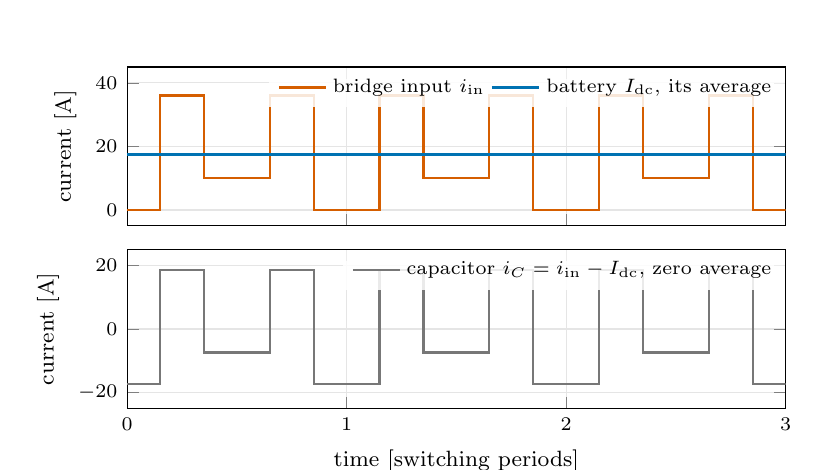
\begin{tikzpicture}
  \pgfplotsset{dcax/.style={width=0.82\textwidth, height=3.6cm, xmin=0, xmax=3,
    xtick={0,1,2,3}, grid=major, grid style={black!10},
    tick label style={font=\scriptsize}, label style={font=\footnotesize},
    legend style={font=\scriptsize, draw=none, fill=white, fill opacity=0.85, text opacity=1,
                  at={(1.0,1.0)}, anchor=north east, legend columns=2}}}
  \begin{axis}[dcax, name=sopra, ymin=-5, ymax=45, ytick={0,20,40}, xticklabels={},
               ylabel={current [A]}]
    % zero vettori: nessuna corrente; vettori attivi: la corrente di una fase o di due
    \addplot[farancio, thick, const plot] coordinates {
      (0,0) (0.15,36) (0.35,10) (0.65,36) (0.85,0)
      (1,0) (1.15,36) (1.35,10) (1.65,36) (1.85,0)
      (2,0) (2.15,36) (2.35,10) (2.65,36) (2.85,0) (3,0)};
    \addlegendentry{bridge input $i_\mathrm{in}$}
    \addplot[fblu, very thick, domain=0:3] {17.4};
    \addlegendentry{battery $I_\mathrm{dc}$, its average}
  \end{axis}
  \begin{axis}[dcax, at={(sopra.south)}, anchor=north, yshift=-3mm, ymin=-25, ymax=25,
               ytick={-20,0,20}, xlabel={time [switching periods]}, ylabel={current [A]}]
    \addplot[fgrigio, thick, const plot] coordinates {
      (0,-17.4) (0.15,18.6) (0.35,-7.4) (0.65,18.6) (0.85,-17.4)
      (1,-17.4) (1.15,18.6) (1.35,-7.4) (1.65,18.6) (1.85,-17.4)
      (2,-17.4) (2.15,18.6) (2.35,-7.4) (2.65,18.6) (2.85,-17.4) (3,-17.4)};
    \addlegendentry{capacitor $i_C = i_\mathrm{in} - I_\mathrm{dc}$, zero average}
  \end{axis}
\end{tikzpicture}

\caption{Who carries what in the DC-link, over three switching periods (shape only).
The bridge draws its current in blocks, one phase current or the sum of two
depending on the active vector; the battery, behind its cable inductance,
supplies only the average; the capacitor supplies the rest, with zero
average and an RMS value that sets its heating.}
\label{fig:dccurrent}
\end{figure}

The capacitor carries the difference between the inverter input current and
the (smooth) DC source current (\cref{fig:dccurrent}). Its RMS value is the quantity that determines
the capacitor's self-heating and therefore its life. A closed-form result for
the two-level bridge is given by Kolar and Round~\cite{kolar_dclink}:
%
\begin{equation}
  \frac{I_{C,\mathrm{rms}}}{I_\mathrm{out,rms}}
  = \sqrt{ 2m\left[\frac{\sqrt{3}}{4\pi}
    + \cos^2\!\varphi\left(\frac{\sqrt{3}}{\pi}-\frac{9}{16}m\right)\right]} .
  \label{eq:kolar}
\end{equation}

\begin{finding}{Two different modulation indices live in this report}
\Cref{eq:kolar} uses $m$ referred to \emph{half} the DC-link,
$m = 2\hat{V}_\mathrm{ph}/\Vdc = 1.07$, which is the convention of the
original derivation. \Cref{eq:svpwm-limit} uses $m$ referred to the full
DC-link, $m = \hat{V}_\mathrm{ph}/\Vdc = 0.534$.

The distinction matters: with $m = 1.07$ the bracket
$\left(\sqrt{3}/\pi - 9m/16\right)$ is \emph{negative}, so at the rated point
the ratio grows as $\cos\varphi$ falls; with $m = 0.534$ it is positive and
the trend reverses. Substituting the wrong one places the rated point on the
wrong branch of the curve.
\end{finding}

Two properties of \cref{eq:kolar} matter for the design. At the \emph{rated}
modulation index, $m = 1.07$, the bracket multiplying $\cos^2\varphi$ is
negative and the ratio grows as $\cos\varphi$ falls: \num{0.447} at the rated
point, \num{0.542} at $\cos\varphi \to 0$. But the modulation index
falls with speed, and the worst case must be sought over the whole
operating envelope, $0 \leq m \leq 1.15$ and $0 \leq \cos\varphi \leq 1$.
There the maximum is at unity power factor, where
$\partial/\partial m$ of the bracket vanishes:
%
\begin{equation}
  m^\ast = \frac{8}{9}\left(\frac{\sqrt{3}}{4\pi}+\frac{\sqrt{3}}{\pi}\right)
         = 0.613,
  \qquad
  \frac{I_{C,\mathrm{rms}}}{I_\mathrm{out,rms}}\bigg|_{\max} = 0.650 ,
\end{equation}
%
that is \SI{19.5}{\ampere} at \SI{30}{\Arms} (\cref{fig:kolar}). The capacitor's worst case is a
low-speed point at full current and unity power factor, not the rated point
(\SI{13.4}{\ampere}) nor the reactive one (\SI{16.9}{\ampere} at $m = 1.15$).

\begin{figure}[htbp]
\centering
% Corrente efficace nel DC-link riferita alla corrente di fase, al variare di
% M_f = V_M/V_DC e del fattore di potenza. Legenda sotto il grafico, etichette
% dei due punti fuori dalle curve.
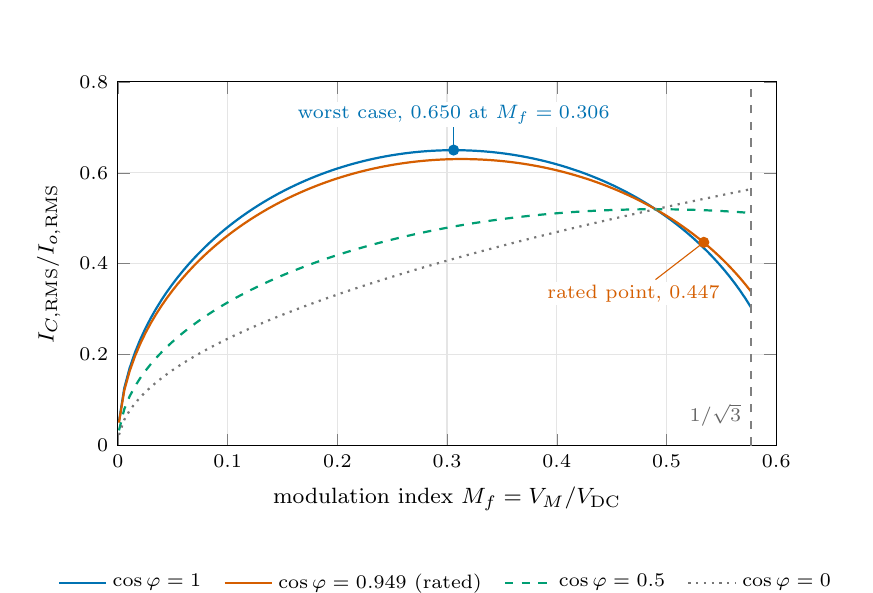
\begin{tikzpicture}
  \begin{axis}[
    width=0.82\textwidth, height=6.2cm,
    xmin=0, xmax=0.6, ymin=0, ymax=0.8,
    xtick={0,0.1,0.2,0.3,0.4,0.5,0.6},
    xticklabel style={/pgf/number format/fixed, /pgf/number format/precision=1},
    scaled x ticks=false,
    xlabel={modulation index $M_f = V_M/\Vdc$},
    ylabel={$I_{C,\mathrm{RMS}}/I_{o,\mathrm{RMS}}$},
    grid=major, grid style={black!10},
    legend columns=4,
    legend style={font=\scriptsize, draw=none, fill=none, at={(0.5,-0.32)}, anchor=north,
                  /tikz/every even column/.append style={column sep=6pt}},
    tick label style={font=\scriptsize}, label style={font=\footnotesize},
    domain=0.001:0.577, samples=120]
    \addplot[fblu, thick] {sqrt(max(0, x*(sqrt(3)/pi + 1*(4*sqrt(3)/pi - 4.5*x))))};
    \addlegendentry{$\cos\varphi = 1$}
    \addplot[farancio, thick] {sqrt(max(0, x*(sqrt(3)/pi + 0.949^2*(4*sqrt(3)/pi - 4.5*x))))};
    \addlegendentry{$\cos\varphi = 0.949$ (rated)}
    \addplot[fverde, thick, dashed] {sqrt(max(0, x*(sqrt(3)/pi + 0.25*(4*sqrt(3)/pi - 4.5*x))))};
    \addlegendentry{$\cos\varphi = 0.5$}
    \addplot[fgrigio, thick, dotted] {sqrt(max(0, x*(sqrt(3)/pi)))};
    \addlegendentry{$\cos\varphi = 0$}
    % limite lineare SVPWM
    \draw[black!50, dashed] (axis cs:0.577,0) -- (axis cs:0.577,0.8);
    \node[font=\scriptsize, black!60, anchor=south east] at (axis cs:0.577,0.02) {$1/\sqrt{3}$};
    % punto nominale e caso peggiore, con le etichette su fondo bianco
    \addplot[only marks, mark=*, mark size=1.8pt, farancio] coordinates {(0.534,0.447)};
    \node[font=\scriptsize, farancio, fill=white, inner sep=1pt, anchor=north] at (axis cs:0.47,0.36) {rated point, 0.447};
    \draw[farancio, thin] (axis cs:0.534,0.447) -- (axis cs:0.49,0.365);
    \addplot[only marks, mark=*, mark size=1.8pt, fblu] coordinates {(0.306,0.650)};
    \node[font=\scriptsize, fblu, fill=white, inner sep=1pt, anchor=south] at (axis cs:0.306,0.70) {worst case, 0.650 at $M_f = 0.306$};
    \draw[fblu, thin] (axis cs:0.306,0.650) -- (axis cs:0.306,0.70);
  \end{axis}
\end{tikzpicture}

\caption{DC-link RMS current relative to the phase current, \cref{eq:kolar}, over
the whole modulation range and four power factors. The rated point sits on
the falling branch of its curve; the worst case of the envelope is a
low-speed point at unity power factor.}
\label{fig:kolar}
\end{figure}

A rule of thumb frequently used in practice sets
$I_{C,\mathrm{rms}} \approx 0.65\,I_\mathrm{out,rms}$. It coincides with the
maximum of \cref{eq:kolar} over the
envelope, which is presumably where it comes from. \Cref{ch:model} checks the
formula against the simulation at the rated modulation index.

The two film capacitors are rated \SI{43.5}{} and \SI{40}{\ampere} RMS at
\SI{85}{\celsius}~\cite{vishay_mkp1848}. At the worst case the larger one
carries about \SI{13.6}{\ampere} of the \SI{19.5}{}, which heats its hotspot
by \SI{1.5}{\celsius}: the binding constraint is the voltage class. Film is chosen over electrolytic for the ripple-current capability
and the life at temperature; the cost is volume, \SI{864}{\gram} and two
packages of \SI{130}{} and \SI{65}{\milli\metre} by \SI{65}{\milli\metre}.

\section{Switching frequency}

The choice of \SI{20}{\kilo\hertz} balances three effects that pull in
different directions. At \SI{20}{\kilo\hertz} the acoustic noise from
magnetostriction in the machine and from the capacitor is above the range
most people hear; \SI{10}{\kilo\hertz} would halve the switching losses but
put a tone in the middle of the audible band, which a passenger vehicle does
not accept. A higher $\fsw$ reduces the current ripple and with it the
harmonic losses in the machine. The switching losses grow linearly with
$\fsw$: \cref{ch:losses} measures the slope at \SI{596}{\micro\joule} per
device per cycle.

\Cref{ch:losses} shows the full sweep from \SI{10}{} to \SI{30}{\kilo\hertz}.
The total loss varies from \SI{90.5}{\watt} to \SI{166.1}{\watt} across
that range, and the junction temperature at the rated point from
\SI{76.9}{\celsius} to \SI{86.8}{\celsius}: at the rated point the design is
not thermally limited anywhere in the range. The limit is at locked rotor
(\cref{sec:lockedrotor}), where the \SI{20}{\kilo\hertz} is held by
requirement and costs its full switching loss on one device. The frequency
is therefore chosen on the acoustic and harmonic-content arguments and then
verified at locked rotor.

\chapter{Modulation and dead time}
\label{ch:modulation}

\section{Modulation}

The modulating signal of each leg is written as the normalised phase
reference plus a common offset $m_0$:
%
\begin{equation}
  m_k = \frac{v_{kN,\mathrm{ref}}}{\Vdc} + m_0 ,
  \qquad m_k \in [0,1] , \qquad k = 1,2,3 .
\end{equation}
%
The offset is the same in the three legs, so it cancels in the line
voltages and does not reach the load. Its choice gives the different
modulations:
\begin{itemize}
  \item sinusoidal PWM (SPWM): $m_0 = 0.5$;
  \item space-vector PWM (SV-PWM):
        %
        \begin{equation}
          m_0 = \frac{1 - \max(\cdot) - \min(\cdot)}{2} ,
          \label{eq:zero-seq}
        \end{equation}
        %
        where $\max(\cdot)$ and $\min(\cdot)$ are the largest and smallest
        of the three normalised references;
  \item discontinuous PWM: $m_0 = 1 - \max(\cdot)$ (DPWM-MAX) or
        $m_0 = -\min(\cdot)$ (DPWM-MIN). One leg at a time is clamped to a
        rail and does not switch.
\end{itemize}

The converter uses SV-PWM. \Cref{fig:modulanti} shows the three modulating
signals against the triangular carrier.

\begin{figure}[H]
\centering
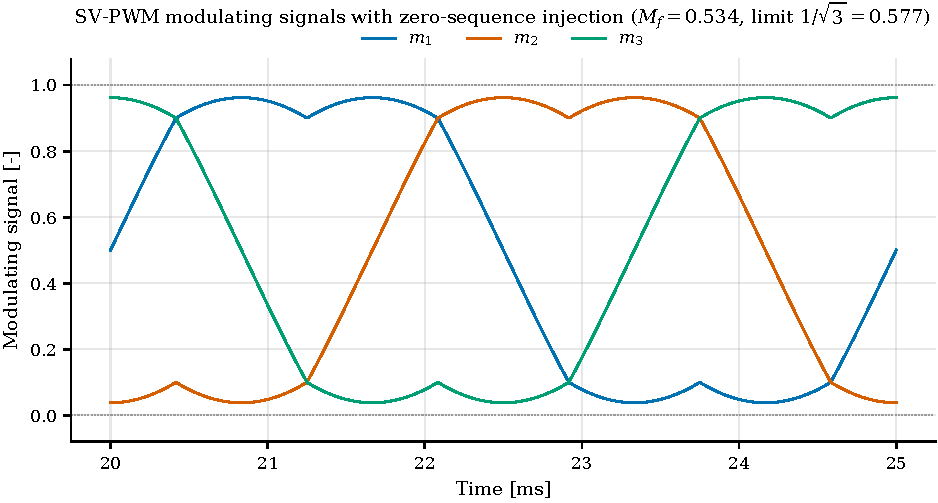
\includegraphics[width=\textwidth]{plecs_05_segnali_modulanti.pdf}
\caption{Modulating signals with the SV-PWM offset of \cref{eq:zero-seq},
against the triangular carrier.}
\label{fig:modulanti}
\end{figure}

\subsection{Choice of the modulation}

\Cref{tab:modulation} and \cref{fig:radar-modulation} compare the three
options.

\begin{table}[H]
\centering
\caption{Carrier-based modulations.}
\label{tab:modulation}
\small
\zebra
\begin{tabularx}{\textwidth}{lYYY}
\toprule
 & SPWM & SV-PWM (chosen) & DPWM \\
\midrule
Offset $m_0$ & 0.5 & $(1-\max-\min)/2$ & $1-\max$ or $-\min$ \\
Maximum linear $M_f$ & 0.500 & 0.577 & 0.577 \\
DC-link utilisation & baseline & +\SI{15.5}{\percent} & +\SI{15.5}{\percent} \\
Switching losses & baseline & baseline & $-\SI{33}{\percent}$ \\
Current ripple & baseline & similar & higher \\
Implementation & simple & one max and one min per period & clamping logic \\
\bottomrule
\end{tabularx}
\end{table}

\begin{figure}[H]
\centering
% Generato da radar.py: non modificare a mano.
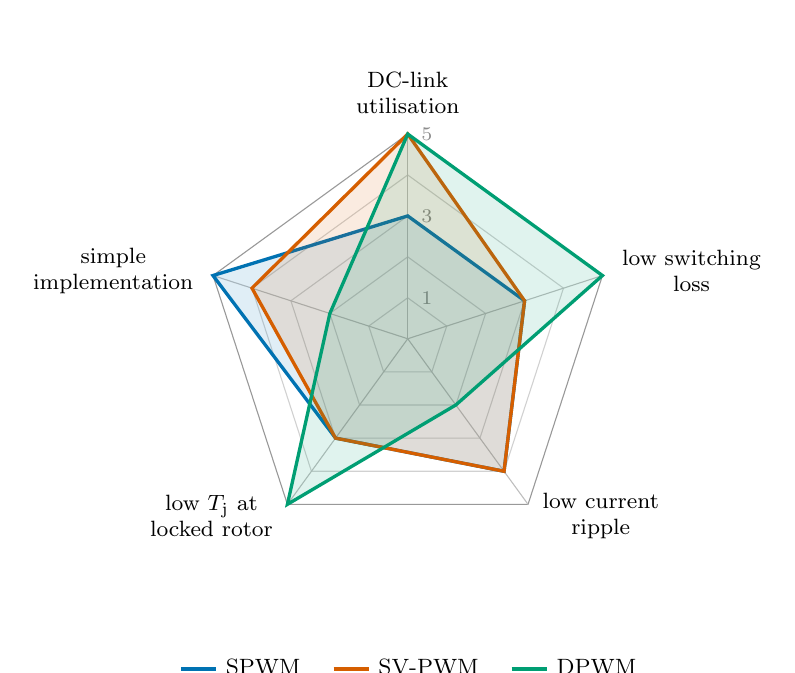
\begin{tikzpicture}[font=\footnotesize]
  \draw[black!18] (0.000,0.520) -- (0.495,0.161) -- (0.306,-0.421) -- (-0.306,-0.421) -- (-0.495,0.161) -- cycle;
  \draw[black!18] (0.000,1.040) -- (0.989,0.321) -- (0.611,-0.841) -- (-0.611,-0.841) -- (-0.989,0.321) -- cycle;
  \draw[black!18] (0.000,1.560) -- (1.484,0.482) -- (0.917,-1.262) -- (-0.917,-1.262) -- (-1.484,0.482) -- cycle;
  \draw[black!18] (0.000,2.080) -- (1.978,0.643) -- (1.223,-1.683) -- (-1.223,-1.683) -- (-1.978,0.643) -- cycle;
  \draw[black!40] (0.000,2.600) -- (2.473,0.803) -- (1.528,-2.103) -- (-1.528,-2.103) -- (-2.473,0.803) -- cycle;
  \draw[black!25] (0,0) -- (0.000,2.600);
  \node[align=center, inner sep=2pt, anchor=south] at (0.000,2.782) {DC-link\\utilisation};
  \draw[black!25] (0,0) -- (2.473,0.803);
  \node[align=center, inner sep=2pt, anchor=west] at (2.646,0.860) {low switching\\loss};
  \draw[black!25] (0,0) -- (1.528,-2.103);
  \node[align=center, inner sep=2pt, anchor=west] at (1.635,-2.251) {low current\\ripple};
  \draw[black!25] (0,0) -- (-1.528,-2.103);
  \node[align=center, inner sep=2pt, anchor=east] at (-1.635,-2.251) {low $T_\mathrm{j}$ at\\locked rotor};
  \draw[black!25] (0,0) -- (-2.473,0.803);
  \node[align=center, inner sep=2pt, anchor=east] at (-2.646,0.860) {simple\\implementation};
  \node[black!45, font=\scriptsize, anchor=west] at (0.050,0.520) {1};
  \node[black!45, font=\scriptsize, anchor=west] at (0.050,1.560) {3};
  \node[black!45, font=\scriptsize, anchor=west] at (0.050,2.600) {5};
  \draw[fblu, very thick, fill=fblu, fill opacity=0.12] (0.000,1.560) -- (1.484,0.482) -- (1.223,-1.683) -- (-0.917,-1.262) -- (-2.473,0.803) -- cycle;
  \draw[farancio, very thick, fill=farancio, fill opacity=0.12] (0.000,2.600) -- (1.484,0.482) -- (1.223,-1.683) -- (-0.917,-1.262) -- (-1.978,0.643) -- cycle;
  \draw[fverde, very thick, fill=fverde, fill opacity=0.12] (0.000,2.600) -- (2.473,0.803) -- (0.611,-0.841) -- (-1.528,-2.103) -- (-0.989,0.321) -- cycle;
  \node[anchor=north] at (0,-3.95) {\tikz[baseline=-0.6ex]\draw[fblu, very thick] (0,0) -- (0.45,0); SPWM \quad \tikz[baseline=-0.6ex]\draw[farancio, very thick] (0,0) -- (0.45,0); SV-PWM \quad \tikz[baseline=-0.6ex]\draw[fverde, very thick] (0,0) -- (0.45,0); DPWM};
\end{tikzpicture}

\caption{Modulations compared on a scale from 1 (worst) to 5 (best); a larger area is better.
Utilisation, switching loss and locked-rotor temperature come from the
numbers of this chapter and of \cref{sec:lrdpwm}; the other axes rank the
three options.}
\label{fig:radar-modulation}
\end{figure}

SV-PWM is chosen for these reasons:
\begin{itemize}
  \item It uses \SI{15.5}{\percent} more of the DC-link voltage than SPWM
        ($M_f$ up to 0.577 instead of 0.500), with the same switching loss.
  \item Its current ripple is the same as SPWM.
  \item It needs only the maximum and the minimum of the three references.
\end{itemize}

DPWM would cut the switching loss by about one third. At the rated point
this is about \SI{23}{\watt} of the \SI{70.6}{\watt} of switching
(\cref{tab:losses}) [estimate]. The junction is at \SI{81.8}{\celsius}, so
the rated point does not need this reduction, and DPWM would increase the
current ripple.

At locked rotor DPWM helps more (\cref{sec:lrdpwm}). If the phase at peak
current is clamped, the hottest junction falls from \SI{111.0}{} to
\SI{93.8}{\celsius}. The design, however, does not count on it:
\begin{itemize}
  \item the modulation is set by the controller, which is outside the
        power stage;
  \item every thermal result of this report uses SV-PWM;
  \item DPWM at low output frequency is listed as a recommendation to the
        controller (\cref{tab:sysassume}), and it is an extra margin.
\end{itemize}

\section{Output waveforms}

\begin{figure}[H]
\centering
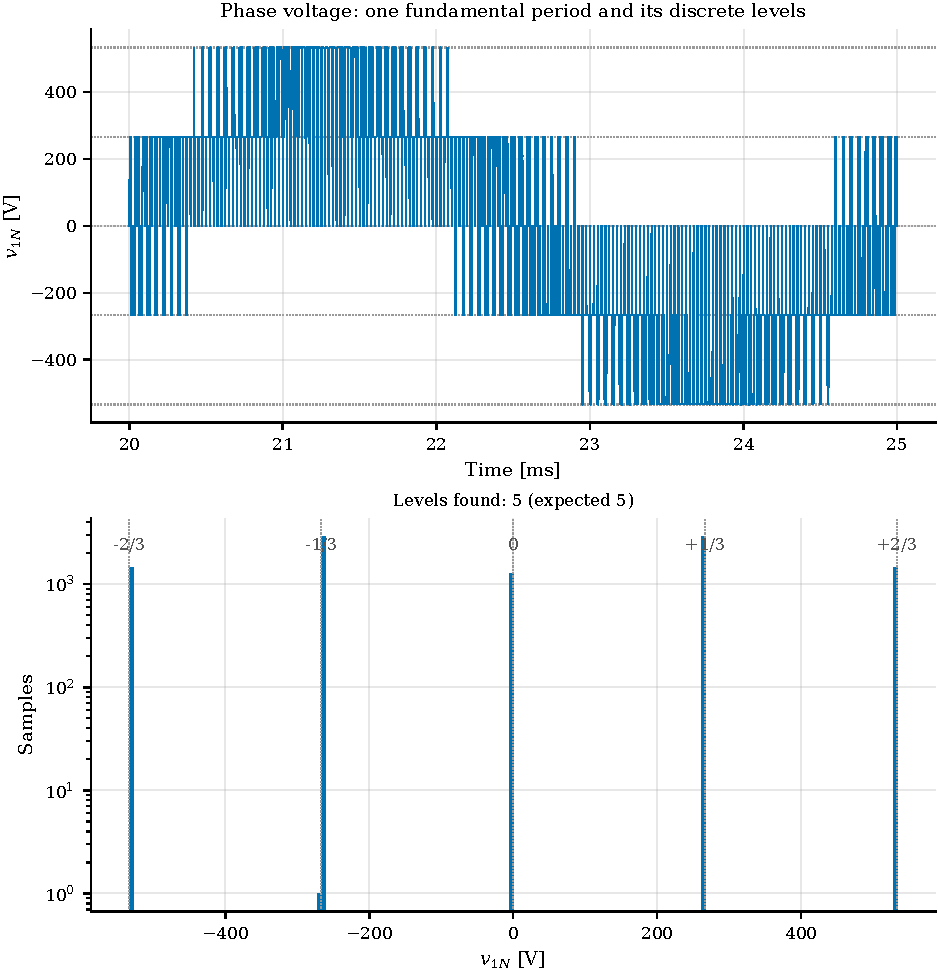
\includegraphics[width=\textwidth]{plecs_02_tensione_di_fase.pdf}
\caption[Phase voltage referred to the load neutral]{Phase voltage $v_{1N}$ referred to the load neutral, with the five
levels $0, \pm\Vdc/3, \pm 2\Vdc/3$.}
\label{fig:tensioni}
\end{figure}

Each pole voltage $v_{k0}$ has only two values, $0$ and $\Vdc$. The load
neutral floats, so the phase voltage $v_{1N} = v_{10} - v_{N0}$ has the five
levels of \cref{fig:tensioni}.

\begin{figure}[H]
\centering
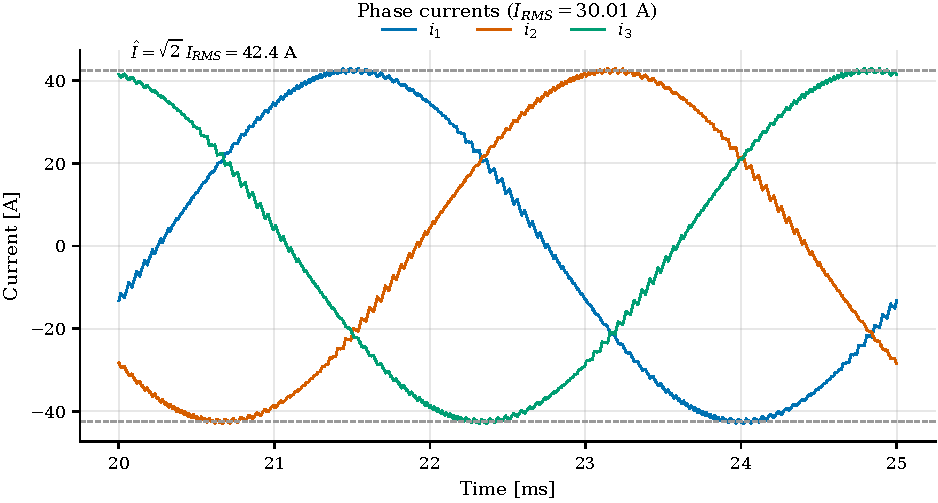
\includegraphics[width=\textwidth]{plecs_03_correnti_di_fase.pdf}
\caption{Phase currents. The switching ripple is \SI{2.463}{\ampere}
peak-to-peak, \SI{5.80}{\percent} of the peak and \SI{0.844}{\percent} in
RMS terms.}
\label{fig:correnti}
\end{figure}

The brief asks for a negligible output current ripple. With the
\SI{2.5}{\milli\henry} load the ripple is:
\begin{itemize}
  \item \SI{2.46}{\ampere} peak-to-peak, \SI{5.8}{\percent} of the peak;
  \item \SI{0.84}{\percent} of the RMS current, equal to the current THD.
\end{itemize}
No output filter is needed. The ripple is inversely proportional to the load
inductance. A motor with a quarter of this inductance would have four times
the ripple and would need an output inductor.

\section{Dead time}
\label{sec:deadtime}

A dead time between the turn-off of one device of a leg and the turn-on of
the other prevents a shoot-through.

\subsection{Sizing}

The worst case is a slow turn-off of one device together with a fast
turn-on of the other. \Cref{tab:deadtime} adds the three contributions:
\begin{itemize}
  \item the difference between the turn-off and turn-on delays of the
        MOSFET;
  \item the pulse-width distortion of the gate signals;
  \item the skew between the gate signals of the two devices.
\end{itemize}

\begin{table}[H]
\centering
\caption{Dead-time budget. Gate-signal tolerances are maxima of a typical
isolated gate driver~\cite{ti_ucc21750}; blue: chosen value.
Device values are typical, read from the switching-time curves
of~\cite{wolfspeed_e3m0016} at the design gate resistances,
\SI{5}{\ohm} at turn-on and \SI{12.5}{\ohm} at turn-off.}
\label{tab:deadtime}
\zebra
\begin{tabular}{lcl}
\toprule
Contribution & Value & Source \\
\midrule
$t_\mathrm{d(off)} - t_\mathrm{d(on)}$ of the MOSFET, $144 - 38$ & \SI{106}{\nano\second} & \cite{wolfspeed_e3m0016} \\
Pulse-width distortion of the gate signals & \SI{30}{\nano\second} & \cite{ti_ucc21750} \\
Skew between the two gate signals & \SI{30}{\nano\second} & \cite{ti_ucc21750} \\
Minimum & \SI{166}{\nano\second} & \\
Minimum with the fall time $t_f = \SI{32}{\nano\second}$ & \SI{198}{\nano\second} & \\
\scelta Chosen & \SI{260}{\nano\second} & factor 1.57 (1.31 with $t_f$) \\
\bottomrule
\end{tabular}
\end{table}

The largest term is the delay of the MOSFET. It grows with the gate
resistance, so the dead time must be checked again whenever $R_g$ changes.
The gate resistances come from the overshoot limit (\cref{sec:kelvin}).

\begin{figure}[H]
\centering
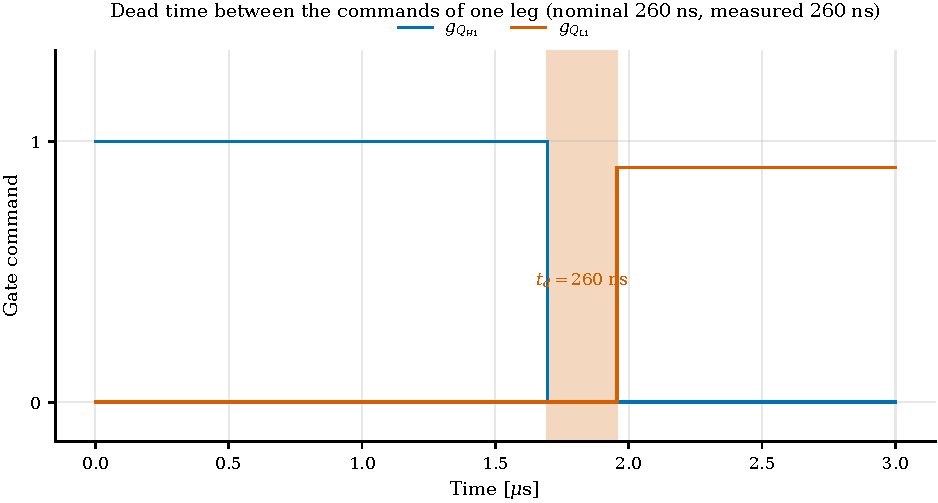
\includegraphics[width=\textwidth]{plecs_06_dead_time.pdf}
\caption{One commutation with the \SI{260}{\nano\second} interval in which
both gate commands are low.}
\label{fig:deadtime}
\end{figure}

\subsection{Loss in the dead time}

During the dead time the phase current flows in the body diode of one
device instead of in its channel. The extra loss is the difference between
the diode drop and the channel drop it replaces:
%
\begin{equation}
  P_\mathrm{dt} = 3 \cdot \big\langle \Delta V(i)\,|i| \big\rangle
  \cdot 2\, t_\mathrm{dead}\, \fsw ,
  \qquad
  \Delta V = V_\mathrm{SD}(i) - v_\mathrm{ch}(i) .
  \label{eq:deadtime-loss}
\end{equation}
%
The factors are:
\begin{itemize}
  \item 3: in each leg one body diode conducts during the dead time,
        chosen by the sign of the phase current;
  \item 2: there are two dead times per switching period;
  \item $\langle\cdot\rangle$: the average over one output period.
\end{itemize}
With the vendor tables of the \device{} at $\Tj = \SI{80}{\celsius}$,
$\Delta V$ averages \SI{3.8}{\volt}. The \SI{260}{\nano\second} dead time
then costs \SI{3.3}{\watt} for the whole converter, about
\SI{2.6}{\percent} of the total loss. \Cref{sec:deadtime-loss} checks this
value with the simulation.

\chapter{Simulation model and validation}
\label{ch:model}

\section{Model structure}

The converter is modelled in PLECS~\cite{plecs}. The model contains:
\begin{itemize}
  \item three half-bridge modules on a common heat sink;
  \item the \SI{200}{\micro\farad} DC-link with its ESR;
  \item a \SI{5}{\micro\henry} source inductance for the battery cables;
  \item an $RL$ load per phase;
  \item the modulator of \cref{ch:modulation}.
\end{itemize}
The devices use the vendor thermal description~\cite{wolfspeed_plecs}. It
gives the conduction and switching losses as tables of current, voltage and
junction temperature. It scales the switching energy with the gate
resistance. The model passes it the design values, \SI{5}{\ohm} at turn-on
and \SI{12.5}{\ohm} at turn-off.

For the \device{} the vendor gives the description in the older two-file
format (MOSFET and body diode), while the model uses the newer single-file
format. A script converts one into the other. It was tested on the
C3M0040120K, which exists in both formats: all \num{579} table values of the
conversion equal the vendor's own single file.

All simulations run from Python through the PLECS XML-RPC interface. Every
figure and number of this report can be reproduced with one command.

\section{Spectra}

PLECS uses a variable time step, so its output is not uniformly sampled. For
the spectra the solver is asked for a uniform grid that covers a whole number
of output periods. The fundamental then falls exactly on one bin and no
window is needed.

\begin{figure}[htbp]
\centering
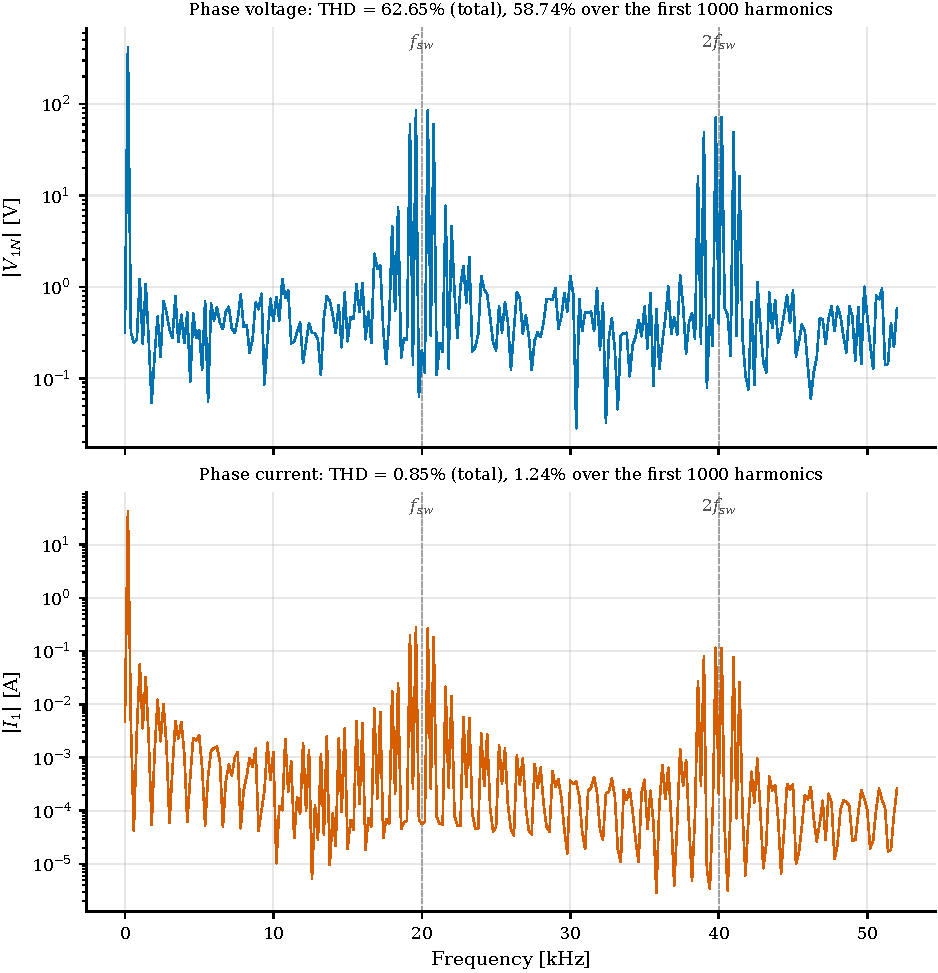
\includegraphics[width=\textwidth]{plecs_07_spettri_fft.pdf}
\caption{Spectra of the phase voltage $v_{1N}$ and of the phase current
$i_1$. The sidebands around \SI{20}{\kilo\hertz} and its multiples are clear
in the voltage. The load inductance attenuates them in the current.}
\label{fig:fft}
\end{figure}

The THD uses the RMS value of the waveform:
%
\begin{equation}
  \mathrm{THD} = \frac{\sqrt{V_\mathrm{rms}^2 - V_1^2}}{V_1} .
  \label{eq:thd}
\end{equation}
%
The phase voltage has a THD of \SI{62.6}{\percent}. A sum truncated at 50
harmonics reaches only \SI{10}{\kilo\hertz}, misses the switching spectrum
and gives about \SI{1}{\percent}. The current THD is \SI{0.85}{\percent}:
the load inductance filters the voltage harmonics.

\section{Check of the vendor loss tables}
\label{sec:losstables}

The losses of \cref{ch:losses} come from the vendor tables, so the tables
are checked against the datasheet. The vendor library has the same device in
two folders: a pair of files (\texttt{MOSFET} and \texttt{Diode}) and a
single file of class \texttt{MOSFET with Diode}. The datasheet gives two
switching energies at the test point (\SI{800}{\volt}, \SI{80.28}{\ampere},
\SI{175}{\celsius}, \SI{2.5}{\ohm}):
\begin{itemize}
  \item free-wheeling through an external SiC diode: $\Eon = \SI{1287}{\micro\joule}$;
  \item free-wheeling through the body diode: $\Eon = \SI{2552}{\micro\joule}$.
\end{itemize}
This design has no external diode, so only the second case applies.
\Cref{tab:losstable-check} compares the table entries with both cases.

\begin{table}[htbp]
\centering
\caption{Vendor table entries against the two datasheet
cases~\cite{wolfspeed_e3m0016,wolfspeed_plecs}.}
\label{tab:losstable-check}
\zebra
\begin{tabular}{lrrrl}
\toprule
Quantity & XML table & SiC diode & Body diode & Matches \\
\midrule
$\Eon$  & \SI{2545.8}{\micro\joule} & \SI{1287}{\micro\joule} & \SI{2552}{\micro\joule} & body diode \\
$\Eoff$ & \SI{784.7}{\micro\joule}  & \SI{805}{\micro\joule}  & \SI{788}{\micro\joule}  & body diode \\
\bottomrule
\end{tabular}
\end{table}

The tables match the body-diode case within \SI{0.24}{\percent} on $\Eon$
and \SI{0.41}{\percent} on $\Eoff$. The name \texttt{MOSFET with Diode}
means a MOSFET modelled together with its own body diode. The tables can
therefore be used without correction.

\section{Validation against the formulas}
\label{sec:validation}

Four checks compare the model with the analytical results.

\subsection{DC-link capacitor current}

The model is run at exactly \SI{30}{\Arms} for eight power factors, with
the modulation amplitude of \SI{427}{\volt}. \Cref{tab:ic-check} compares
the capacitor current with \cref{eq:icrms}.

\begin{table}[htbp]
\centering
\caption{DC-link capacitor RMS current at \SI{30}{\Arms}: simulation and
\cref{eq:icrms}.}
\label{tab:ic-check}
\zebra
\begin{tabular}{rrrr}
\toprule
$\cos\varphi$ & Simulated [\si{\ampere}] & Formula [\si{\ampere}] & Difference \\
\midrule
0.02 & 16.28 & 16.28 & \SI{0.0}{\percent} \\
0.10 & 16.25 & 16.24 & \SI{0.1}{\percent} \\
0.30 & 16.01 & 16.01 & \SI{0.0}{\percent} \\
0.50 & 15.56 & 15.53 & \SI{0.2}{\percent} \\
0.70 & 14.89 & 14.79 & \SI{0.7}{\percent} \\
0.87 & 14.15 & 13.91 & \SI{1.7}{\percent} \\
0.95 & 13.74 & 13.40 & \SI{2.5}{\percent} \\
1.00 & 14.47 & 12.67 & \SI{14}{\percent} \\
\bottomrule
\end{tabular}
\end{table}

The agreement is within \SI{2.5}{\percent} up to $\cos\varphi = 0.95$. At
$\cos\varphi = 1$ the difference is larger. The load at this point has only
\SI{0.1}{\milli\henry}, so the output current has a large ripple. The
formula of the course assumes a negligible ripple.

At the worst case of \cref{sec:dclink} ($\cos\varphi = 1$, $M_f = 0.306$) the
formula gives \SI{19.49}{\ampere}. The model with the \SI{5}{\micro\henry}
source gives about \SI{19.9}{\ampere}.

\subsection{Switching loss against frequency}

The switching loss must be linear in $\fsw$ and zero at $\fsw = 0$. A sweep
from \SI{10}{} to \SI{30}{\kilo\hertz} gives \SI{596.5}{\micro\joule} per
device and per cycle, with $R^2 = \num{1.0000}$ and an intercept of
\SI{-1.01}{\watt}.

\subsection{Conduction loss}

The conduction loss was recomputed in Python. The script integrates the
vendor voltage-drop tables over a sinusoidal current of \SI{30.006}{\Arms},
at the junction temperature of the thermal loop, \SI{81.84}{\celsius}:
\begin{itemize}
  \item channels: \SI{54.56}{\watt};
  \item extra loss in the dead time (\cref{eq:deadtime-loss}): \SI{3.21}{\watt};
  \item total: \SI{57.77}{\watt}, against \SI{57.64}{\watt} from PLECS
        (\SI{0.23}{\percent}).
\end{itemize}
The same tables are used in \cref{ch:thermal,ch:losses} for the estimates
made outside PLECS.

\subsection{Steady-state analysis of PLECS}

The thermal results of this report come from time-domain runs. The case
temperature is iterated until losses and temperature agree. PLECS also has a
steady-state analysis, as the brief suggests. It finds the periodic solution
directly and is a second method. The period to give is $1/f_\mathrm{ref}$,
the period of the output, not $1/\fsw$. With $1/\fsw$ the analysis returned
\SI{2}{\watt} of total loss.

With the correct period, the final model gives:
\begin{itemize}
  \item steady-state analysis: \SI{128.52}{\watt} and $\Tj = \SI{81.89}{\celsius}$;
  \item time-domain method: \SI{128.09}{\watt} and $\Tj = \SI{81.84}{\celsius}$.
\end{itemize}
The difference is \SI{0.33}{\percent} on the loss and \SI{0.05}{\celsius}
on the junction. Over the whole sweep of $\Rthcs$ of \cref{ch:thermal}, from
\SI{0.2}{} to \SI{1.2}{\celsius\per\watt}, the two methods agree within
\SI{0.35}{\percent} and \SI{0.12}{\celsius}.

The steady-state analysis has one limit. It uses one case resistance shared
by the six devices, which is correct at the rated point because their losses
are equal. At locked rotor it gives \SI{90.6}{\celsius} for the hottest
junction, against \SI{111.1}{\celsius} with one resistance per device
(\cref{sec:lockedrotor}). Locked rotor therefore uses the per-device method.

\section{DC-link ripple}

\begin{figure}[htbp]
\centering
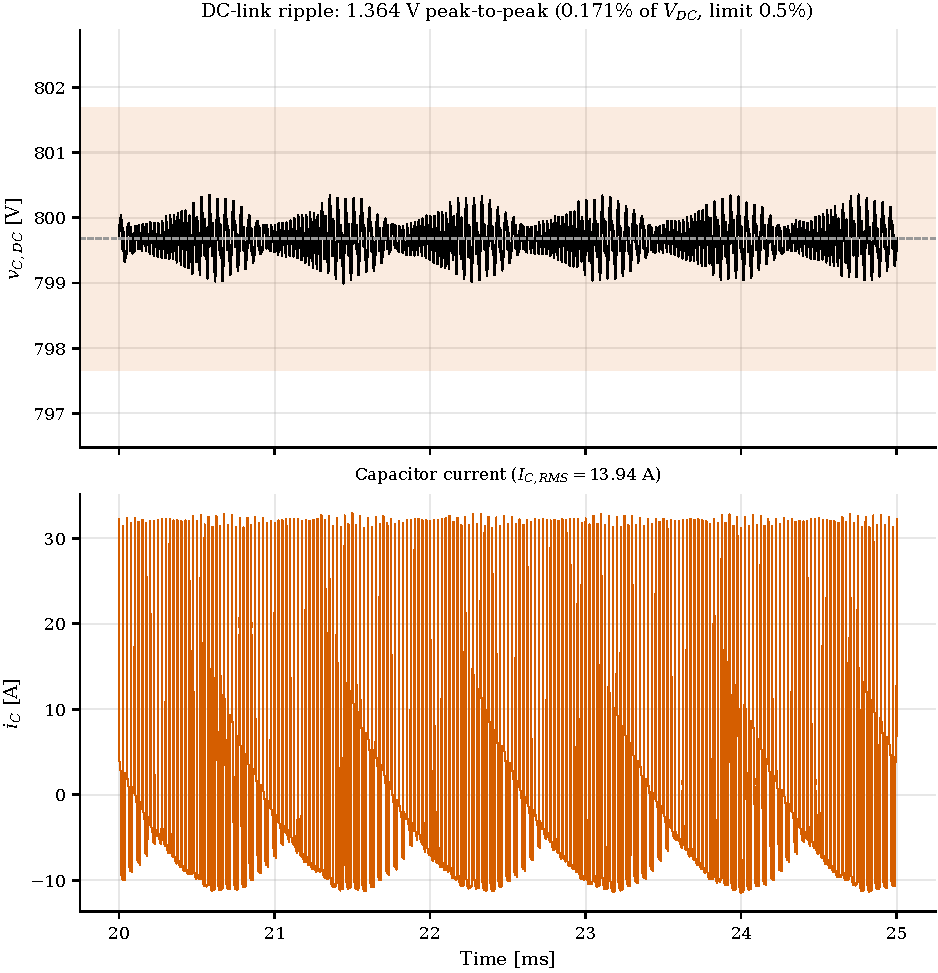
\includegraphics[width=\textwidth]{plecs_04_ripple_dc_link.pdf}
\caption{DC-link voltage ripple at the rated point, with the
\SI{5}{\micro\henry} source inductance: \SI{1.36}{\volt} peak-to-peak on
\SI{800}{\volt}, that is \SI{0.17}{\percent}, against the
\SI{0.5}{\percent} limit.}
\label{fig:ripple}
\end{figure}

The ripple at the rated point is \SI{1.36}{\volt}. Over the whole operating
range the worst case is \SI{2.86}{\volt}, inside the \SI{4}{\volt} limit
(\cref{sec:dclink}). The model with an ideal voltage source instead of the
\SI{5}{\micro\henry} cables would give \SI{0.43}{\volt}: the ideal source
absorbs part of the ripple current, so the cable inductance must be kept in
the model.

\chapter{Loss analysis}
\label{ch:losses}

\section{Loss budget at the design point}

\begin{table}[htbp]
\centering
\caption[Loss budget at the design point]{Loss budget at \SI{800}{\volt}, \SI{30}{\Arms}, \SI{20}{\kilo\hertz},
$\cos\varphi = 0.949$ (\cref{eq:powerfactor}), $R_{g,\mathrm{on}}/R_{g,\mathrm{off}}
= \SI{5}{}/\SI{12.5}{\ohm}$, dead time \SI{260}{\nano\second}, with the
thermal loop closed as described in \cref{ch:thermal}.}
\label{tab:losses}
\begin{tabular}{lrl}
\toprule
Contribution & Value & Notes \\
\midrule
Channel conduction              & \SI{54.4}{\watt} & \\
Body-diode surplus (dead time)  & \SI{3.2}{\watt} & already inside $P_\mathrm{cond}$ \\
\midrule
\textbf{Total conduction} $P_\mathrm{cond}$ & \textbf{\SI{57.6}{\watt}} & \\
\textbf{Switching} $P_\mathrm{sw}$          & \textbf{\SI{70.5}{\watt}}  & \\
\midrule
\textbf{Total} $P_\mathrm{tot}$ & \textbf{\SI{128.1}{\watt}} & \\
Per device                      & \SI{21.3}{\watt} & six devices \\
Switching energy per device     & \SI{596.5}{\micro\joule} & per cycle \\
\textbf{Output power} & \SI{25.48}{\kilo\watt} & active, \cref{eq:active-sim} \\
\textbf{Efficiency} & \textbf{\SI{99.50}{\percent}} & $P_\mathrm{out}/(P_\mathrm{out}+P_\mathrm{tot})$ \\
\bottomrule
\end{tabular}
\end{table}

Switching is \SI{55}{\percent} of the total, an unusual share for a SiC
MOSFET at \SI{20}{\kilo\hertz}. The \SI{16}{\milli\ohm} device makes
conduction small (\SI{57.6}{\watt} against the \SI{151}{\watt} of the
\SI{40}{\milli\ohm} device of the first iterations), but the overshoot
criterion of \cref{sec:kelvin} demands \SI{12.5}{\ohm} at turn-off, and the
tables scale the switching energy with it. The trade is still a good one:
the total is \SI{128}{\watt} against \SI{178}{\watt}, and the locked-rotor
temperature, which is what selected the device, is \SI{30}{\celsius} lower
(\cref{sec:lockedrotor}).

\section{Frequency dependence}

\begin{figure}[htbp]
\centering
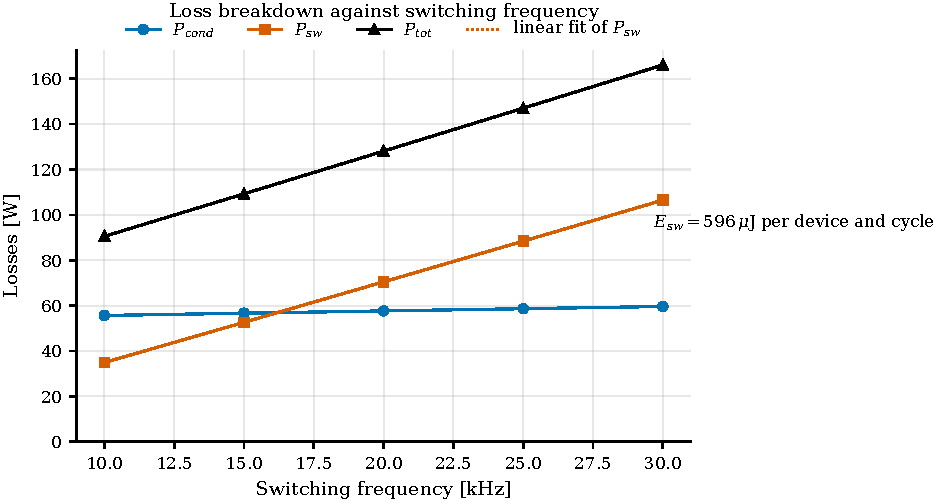
\includegraphics[width=\textwidth]{plecs_08_perdite_vs_fsw.pdf}
\caption{Conduction, switching and total losses against switching frequency.
Conduction is nearly constant, switching is linear in $\fsw$.}
\label{fig:perdite-fsw}
\end{figure}

\begin{table}[htbp]
\centering
\caption{Losses and junction temperature at the rated point against switching
frequency.}
\label{tab:sweep-fsw}
\begin{tabular}{lrrrrr}
\toprule
$\fsw$ & $P_\mathrm{cond}$ & $P_\mathrm{sw}$ & $P_\mathrm{tot}$ & $\Tj$ & Margin \\
\midrule
\SI{10}{\kilo\hertz} & \SI{55.6}{\watt} & \SI{34.9}{\watt} & \SI{90.5}{\watt} & \SI{76.9}{\celsius} & \SI{73.1}{\celsius} \\
\SI{15}{\kilo\hertz} & \SI{56.6}{\watt} & \SI{52.6}{\watt} & \SI{109.3}{\watt} & \SI{79.4}{\celsius} & \SI{70.6}{\celsius} \\
\textbf{\SI{20}{\kilo\hertz}} & \textbf{\SI{57.6}{\watt}} & \textbf{\SI{70.5}{\watt}} & \textbf{\SI{128.1}{\watt}} & \textbf{\SI{81.8}{\celsius}} & \textbf{\SI{68.2}{\celsius}} \\
\SI{25}{\kilo\hertz} & \SI{58.6}{\watt} & \SI{88.4}{\watt} & \SI{147.0}{\watt} & \SI{84.3}{\celsius} & \SI{65.7}{\celsius} \\
\SI{30}{\kilo\hertz} & \SI{59.6}{\watt} & \SI{106.5}{\watt} & \SI{166.1}{\watt} & \SI{86.8}{\celsius} & \SI{63.2}{\celsius} \\
\bottomrule
\end{tabular}
\end{table}

Conduction losses are not exactly constant across the sweep: they rise by
\SI{4.0}{\watt} from \SI{10}{} to \SI{30}{\kilo\hertz}. The cause is the
thermal feedback: more switching loss raises the junction temperature, which raises $\Rdson$, which raises the conduction
loss.

\section{Dependence on the load power factor}
\label{sec:pfsweep}

The brief asks for the rated current at any load power factor. The sweep of
$\cos\varphi$ from \num{0.02} to \num{1} that validates the DC-link current
(\cref{sec:validation}) was run with the losses and the thermal loop as well,
at the rated modulation amplitude and on the ideal cold plate.
\Cref{tab:sweep-pf} gives the result.

\begin{table}[htbp]
\centering
\caption{Losses and junction temperature against load power factor, at
\SI{800}{\volt}, \SI{20}{\kilo\hertz}, modulation amplitude \SI{427}{\volt}.
The last two columns scale each point to exactly \SI{30}{\Arms}, with
conduction proportional to $I^2$ and switching to $I$ [estimate].}
\label{tab:sweep-pf}
\small
\begin{tabular}{rrrrrrrr}
\toprule
 & $I_\mathrm{rms}$ & $P_\mathrm{cond}$ & $P_\mathrm{sw}$ & $P_\mathrm{tot}$ & $\Tj$ & $P_\mathrm{tot}$ at \SI{30}{\Arms} & $\Tj$ at \SI{30}{\Arms} \\
$\cos\varphi$ & [\si{\ampere}] & [\si{\watt}] & [\si{\watt}] & [\si{\watt}] & [\si{\celsius}] & [\si{\watt}] & [\si{\celsius}] \\
\midrule
1.00 & 30.94 & 61.8 & 75.7 & 137.6 & 83.1 & 131.5 & 82.3 \\
0.87 & 30.04 & 57.7 & 70.6 & 128.3 & 81.9 & 128.1 & 81.8 \\
0.50 & 30.18 & 57.9 & 71.0 & 128.9 & 81.9 & 127.8 & 81.8 \\
0.20 & 30.30 & 58.0 & 71.3 & 129.3 & 82.0 & 127.5 & 81.8 \\
0.10 & 30.34 & 58.2 & 71.6 & 129.7 & 82.1 & 127.7 & 81.8 \\
0.02 & 30.36 & 58.2 & 71.6 & 129.8 & 82.1 & 127.6 & 81.8 \\
\bottomrule
\end{tabular}
\end{table}

At a fixed modulation amplitude the load current drifts between \SI{30.0}{}
and \SI{30.9}{\ampere} with the load, so the raw columns mix two effects.
Brought to \SI{30}{\Arms} the losses are \SIrange{127.5}{128.1}{\watt} for
every power factor below \num{0.9}, which is the rated-point value of
\cref{tab:losses}, and the junction stays at \SI{81.8}{\celsius}. The
worst case for the losses is unity power factor, at about \SI{131.5}{\watt}
(\SI{+2.7}{\percent}) and \SI{82.3}{\celsius}: half a kelvin above the rated
point. The rated current is therefore met at any power factor with no change
to the thermal result, and the worst case of the power stage remains the
stalled motor of \cref{sec:lockedrotor}.

\section{The dead-time loss}
\label{sec:deadtime-loss}

\Cref{eq:deadtime-loss} estimates the cost of the dead time analytically. The
simulation provides an independent measurement, but obtaining it requires
care, because the dead time does two things at once: it adds the body-diode
drop \emph{and} it reduces the effective duty cycle, and therefore the
current. At constant modulation depth the two effects nearly cancel and the
conduction loss appears insensitive to the dead time. Re-trimming the
modulation depth to hold the phase current constant separates them:

\begin{table}[htbp]
\centering
\caption{Conduction loss against dead time at constant phase current
(\SI{30.366}{\Arms}), thermal boundary at the \SI{65}{\celsius} coolant.}
\label{tab:deadtime-measured}
\begin{tabular}{lrrr}
\toprule
$t_\mathrm{dead}$ & Modulation amplitude & $P_\mathrm{cond}$ & $\Delta$ \\
\midrule
0                      & \SI{427.000}{\volt} & \SI{52.972}{\watt} & --- \\
\SI{100}{\nano\second} & \SI{428.945}{\volt} & \SI{54.269}{\watt} & \SI{+1.297}{\watt} \\
\textbf{\SI{260}{\nano\second}} & \SI{432.062}{\volt} & \SI{56.343}{\watt} & \textbf{\SI{+3.370}{\watt}} \\
\SI{1}{\micro\second}  & \SI{446.363}{\volt} & \SI{65.743}{\watt} & \SI{+12.770}{\watt} \\
\bottomrule
\end{tabular}
\end{table}

The response is linear, as it must be, and agrees with
\cref{eq:deadtime-loss}, which gives \SIrange{3.26}{3.36}{\watt} at
\SI{260}{\nano\second} for junction temperatures between \SI{80}{} and
\SI{60}{\celsius}: within \SI{3}{\percent}. The \SI{260}{\nano\second} that
the gate resistances impose (\cref{sec:deadtime}) therefore cost
\SI{3.4}{\watt}, \SI{2.6}{\percent} of the budget and a small price; the larger cost of the longer dead time is the
\SI{1.2}{\percent} of fundamental voltage it removes, which the modulation
amplitude of \SI{427}{\volt} restores.

\begin{finding}{The first dead-time estimate was wrong by a factor of 2.3}
An earlier calculation in this work, on the device of the first iterations,
gave \SI{3.2}{\watt} against \SI{1.4}{\watt} from the corrected formula
(\SI{1.5}{\watt} measured), through two
compounding errors. It multiplied by six devices, where only three conduct
during the dead time, one per leg, chosen by the sign of the phase current.
And it used the body diode's \emph{absolute} forward drop instead of the
\emph{difference} against the channel it replaces, at the actual junction
temperature.

Worse, the \SI{3.2}{\watt} was about to be \emph{added} to the simulated
budget. It should not be: the model applies the gate-off conduction table
during the dead time, so this loss is already inside $P_\mathrm{cond}$.
Adding it would have been a double count.
\end{finding}

The dead-time penalty \emph{decreases} with temperature, from \SI{3.36}{\watt} at
\SI{60}{\celsius} to \SI{3.11}{\watt} at \SI{110}{\celsius}
(\cref{eq:deadtime-loss} on the vendor tables). The body diode's forward
voltage has a negative temperature coefficient while the channel resistance
has a positive one, so the difference $\Delta V$ that the dead time costs
shrinks, from \SI{3.94}{} to \SI{3.64}{\volt}, as the device heats up.

\section{Switching cell: SPICE study}
\label{sec:kelvin}

A double-pulse test of a single switching cell was simulated in
LTspice~\cite{ltspice} using the official Wolfspeed
model~\cite{wolfspeed_spice} of the \device{}, to obtain what a table-based
model cannot give: the voltage overshoot at the die, the gate resistance
that keeps it within the criterion of \cref{sec:vhierarchy}, and the value of
the Kelvin source connection. The test point is the worst the converter is
ever asked to switch in operation: \SI{950}{\volt}, the overvoltage trip,
and \SI{60}{\ampere}, the overload trip, at \SI{175}{\celsius}, with the
driver's \SI{-5}{}/\SI{+15}{\volt} and separate turn-on and turn-off
resistors.

\begin{finding}{The first bench measured a bus that was still charging}
The first version of the bench imposed the load current as an initial
condition, which is the usual shortcut. When the solver failed to find the
initial operating point, which happened silently in most runs, it started
from a discharged DC-link and a gate at \SI{0}{\volt}: at the turn-off edge
the bus was at \SI{814}{\volt} and still rising. Every overshoot obtained
that way was wrong, and the one that mattered most was optimistic: the gate
resistance it suggested, \SI{5}{\ohm}, gives \SI{1133}{\volt} at the die
when the test is done properly. The bench now performs a real double pulse,
with a first pulse of \SI{6.25}{\micro\second} that ramps the load current
from zero, and every run is rejected unless bus and current are within
\SI{2}{} and \SI{5}{\percent} of their test values just before the edge.
\end{finding}

\begin{figure}[htbp]
\centering
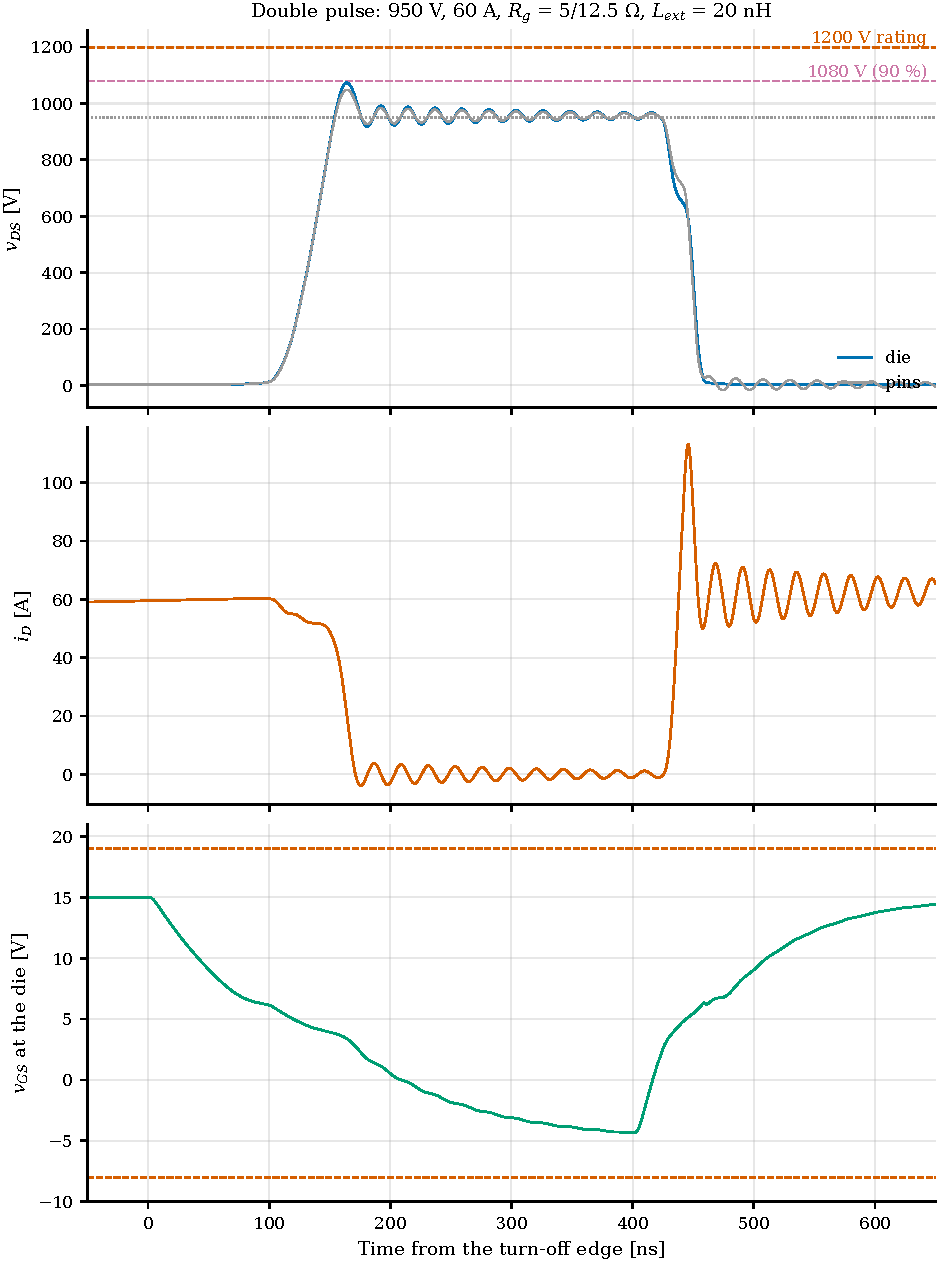
\includegraphics[width=\textwidth]{spice_12_dpt_forme_donda.pdf}
\caption{Double-pulse waveforms at \SI{950}{\volt}, \SI{60}{\ampere},
$R_{g,\mathrm{on}}/R_{g,\mathrm{off}} = \SI{5}{}/\SI{12.5}{\ohm}$,
\SI{20}{\nano\henry}: drain--source voltage at the die and at the pins,
drain current, and gate--source voltage at the die.}
\label{fig:dpt}
\end{figure}

\subsection{Gate drive levels}
\label{sec:negbias}

The gate is driven between $+\SI{15}{\volt}$ and $-\SI{5}{\volt}$, a swing of
\SI{20}{\volt}. The negative level keeps the off device off while its
opposite is turned on: the Miller current injected through $C_\mathrm{gd}$
raises the off gate by
%
\begin{equation}
  \Delta V_\mathrm{GS} = C_\mathrm{gd,eff}\,\frac{\mathrm{d}v}{\mathrm{d}t}\,R
  \left[1 - \exp\!\left(-\frac{t}{R\,C_\mathrm{iss}}\right)\right].
  \label{eq:miller}
\end{equation}
%
With $C_\mathrm{gd,eff} = Q_\mathrm{gd}/V_\mathrm{DS} = \SI{81}{\pico\farad}$,
$C_\mathrm{iss} = \SI{6922}{\pico\farad}$, the turn-on slope that the
double-pulse simulation gives for the opposite device,
\SI{31.4}{\volt\per\nano\second}, and the \SI{15.4}{\ohm} of the off path,
the gate of the off device reaches $+\SI{3.35}{\volt}$ at a bias of
$-\SI{5}{\volt}$, above the \SI{1.8}{\volt} minimum threshold. The active
Miller clamp of the driver brings it to $+\SI{0.58}{\volt}$, a margin of
\SI{1.22}{\volt}; at the datasheet's typical $-\SI{4}{\volt}$ the margin
would be \SI{0.22}{\volt}. The closed form is a bound, and the simulation,
which resolves the internal gate network, keeps the die \SIrange{4}{5}{\volt}
lower. The $-\SI{5}{\volt}$ leaves \SI{3}{\volt} to the absolute maximum of
$-\SI{8}{\volt}$~\cite{wolfspeed_e3m0016} and is what a standard isolated
gate-drive supply delivers without an extra regulator.

\subsection{Gate resistance: fixed by the overshoot criterion}

\begin{table}[htbp]
\centering
\caption{Peak voltage at the die against gate resistance ($R_{g,\mathrm{on}}
= R_{g,\mathrm{off}}$ in the sweep), \SI{950}{\volt}, \SI{60}{\ampere},
\SI{20}{\nano\henry}. Limit \SI{1080}{\volt}.}
\label{tab:rgsweep}
\begin{tabular}{rrrrr}
\toprule
$R_g$ & Device turn-off & Opposite diode recovery & $\Eon$ & $\Eoff$ \\
\midrule
\SI{2.5}{\ohm}  & \SI{1195}{\volt} & \SI{1202}{\volt} & \SI{744}{\micro\joule}  & \SI{389}{\micro\joule} \\
\SI{5}{\ohm}    & \SI{1133}{\volt} & \textbf{\SI{1048}{\volt}} & \SI{952}{\micro\joule}  & \SI{650}{\micro\joule} \\
\SI{7.5}{\ohm}  & \SI{1106}{\volt} & \SI{1039}{\volt} & \SI{1182}{\micro\joule} & \SI{919}{\micro\joule} \\
\SI{10}{\ohm}   & \SI{1087}{\volt} & \SI{995}{\volt}  & \SI{1383}{\micro\joule} & \SI{1178}{\micro\joule} \\
\SI{12.5}{\ohm} & \textbf{\SI{1073}{\volt}} & \SI{981}{\volt} & \SI{1587}{\micro\joule} & \SI{1448}{\micro\joule} \\
\SI{15}{\ohm}   & \SI{1061}{\volt} & \SI{977}{\volt}  & \SI{1814}{\micro\joule} & \SI{1739}{\micro\joule} \\
\SI{20}{\ohm}   & \SI{1045}{\volt} & \SI{956}{\volt}  & \SI{2246}{\micro\joule} & \SI{2267}{\micro\joule} \\
\bottomrule
\end{tabular}
\end{table}

The two edges are governed by different resistors. The overshoot at turn-off
belongs to the device's own turn-off, and it sets $R_{g,\mathrm{off}}$: the
first value below \SI{1080}{\volt} is \SI{12.5}{\ohm}. The overshoot at
turn-on appears on the \emph{opposite} device, as its body diode recovers,
and it sets $R_{g,\mathrm{on}}$: \SI{5}{\ohm} already gives
\SI{1048}{\volt}. The driver has separate source and sink outputs, so the
two can differ, and the design uses \SI{5}{\ohm} at turn-on and
\SI{12.5}{\ohm} at turn-off. At that pair the die reaches
\SI{1073.5}{\volt} at turn-off and \SI{1050}{\volt} at recovery.

The margin at turn-off is six and a half volts on a switching peak at
\SI{90}{\percent} of the rating, with the overvoltage trip and the overload
trip at the same time, the layout at its inductance limit and the voltage
read at the die. Raising $R_{g,\mathrm{off}}$
to \SI{15}{\ohm} would buy twelve more volts for \SI{4}{\watt} of loss and
\SI{2}{\celsius} at locked rotor; the thermal margin at a \SI{70}{\celsius}
coolant was judged the scarcer of the two.

\subsection{Overshoot and loop inductance}

\begin{table}[htbp]
\centering
\caption{Peak voltage at turn-off against external loop inductance,
\SI{950}{\volt}, \SI{60}{\ampere}, \SI{5}{}/\SI{12.5}{\ohm}.}
\label{tab:overshoot}
\begin{tabular}{lrrrr}
\toprule
$L_\mathrm{ext}$ & At the die & At the pins & Fraction of rating & Implied $\mathrm{d}i/\mathrm{d}t$ \\
\midrule
\SI{10}{\nano\henry} & \SI{1044.2}{\volt} & \SI{1017.9}{\volt} & \SI{87.0}{\percent} & \SI{3.82}{\ampere\per\nano\second} \\
\SI{20}{\nano\henry} & \SI{1073.5}{\volt} & \SI{1048.6}{\volt} & \SI{89.5}{\percent} & \SI{3.57}{\ampere\per\nano\second} \\
\SI{50}{\nano\henry} & \SI{1147.8}{\volt} & \SI{1126.0}{\volt} & \SI{95.6}{\percent} & \SI{3.06}{\ampere\per\nano\second} \\
\bottomrule
\end{tabular}
\end{table}

The die sees \SIrange{22}{26}{\volt} more than the pins at every
inductance: that is the drop across the package's own drain and source
inductance, and it is why the criterion is taken at the die. The implied
current slope is computed over the external inductance \emph{plus} the
package, $L_d + L_{s2} + L_v = \SI{7.32}{\nano\henry}$ per device in the
model, \SI{14.6}{\nano\henry} for the two devices in series; counted that
way it stays within \SI{25}{\percent} across a fivefold change of the
external inductance, as it should for a fixed gate drive.

\paragraph{Where C2 fails.} Three points bracket the design
value but do not say where the criterion is lost, and that is the number
the finished board has to be checked against. A finer sweep around
\SI{20}{\nano\henry} gives it:

\begin{table}[htbp]
\centering
\caption{Fine sweep of the external loop inductance around the limit,
\SI{950}{\volt}, \SI{60}{\ampere}, \SI{5}{}/\SI{12.5}{\ohm}, peak at the die.}
\label{tab:lthreshold}
\begin{tabular}{lrr}
\toprule
$L_\mathrm{ext}$ & Turn-off & Recovery, opposite device \\
\midrule
\SI{20}{\nano\henry} & \SI{1073.5}{\volt} & \SI{1050.0}{\volt} \\
\SI{21}{\nano\henry} & \SI{1074.2}{\volt} & \SI{1053.0}{\volt} \\
\SI{22}{\nano\henry} & \SI{1079.0}{\volt} & \SI{1066.6}{\volt} \\
\SI{23}{\nano\henry} & \SI{1080.6}{\volt} & \SI{1073.7}{\volt} \\
\SI{24}{\nano\henry} & \SI{1083.3}{\volt} & \SI{1083.9}{\volt} \\
\SI{26}{\nano\henry} & \SI{1088.5}{\volt} & \SI{1104.2}{\volt} \\
\bottomrule
\end{tabular}
\end{table}

C2 fails at \SI{22.6}{\nano\henry} at turn-off and at
\SI{23.6}{\nano\henry} on recovery. The margin on the layout limit is
therefore \SI{2.6}{\nano\henry}, \SI{13}{\percent}; with the \SI{2}{\volt}
scatter between the converging variants of the model and a local slope of
\SIrange{1.6}{2.7}{\volt\per\nano\henry}, the threshold is known to about
$\pm\SI{1}{\nano\henry}$. Beyond \SI{23}{\nano\henry} the recovery peak rises at
\SI{10}{\volt\per\nano\henry}, four times faster than the turn-off peak,
and it is set by $R_{g,\mathrm{on}}$, not $R_{g,\mathrm{off}}$: a board
that lands above \SI{23}{\nano\henry} cannot be rescued by the turn-off
resistor alone, and both resistors, the losses and the locked-rotor result
would have to be recomputed.

\begin{finding}{The layout limit is not the whole loop}
The \SI{20}{\nano\henry} of \cref{ch:layout} is the
\emph{PCB-attributable} inductance. The packages add \SI{14.6}{\nano\henry}
that no layout can remove, so the real commutation loop would measure around
\SI{35}{\nano\henry} at the limit; the frozen board, extracted, gives about
\SI{23}{\nano\henry} (\cref{sec:loopextract}). Anyone extracting parasitics from the finished board
and comparing against ``\SI{20}{\nano\henry}'' will find a factor of 1.7 and
conclude, wrongly, that the layout failed. The converse also holds: since the
gate resistance was chosen at \SI{20}{\nano\henry} of PCB inductance, a board
above that value invalidates the overshoot verification.
\end{finding}

\subsection{What the fourth pin is worth}

\begin{table}[htbp]
\centering
\caption{Switching energy with the driver return on the Kelvin pin versus the
power source pin, at the design point.}
\label{tab:kelvin}
\begin{tabular}{lrrrr}
\toprule
Driver return & $\Eon$ & $\Eoff$ & Total & Peak $V_\mathrm{GS}$ at the die \\
\midrule
\textbf{Kelvin pin (TO-247-4)} & \SI{966}{\micro\joule} & \SI{1457}{\micro\joule} & \textbf{\SI{2424}{\micro\joule}} & \SI{15.02}{\volt} \\
Power source pin (TO-247-3)    & \SI{1730}{\micro\joule} & \SI{1761}{\micro\joule} & \SI{3490}{\micro\joule} & \SI{15.29}{\volt} \\
\bottomrule
\end{tabular}
\end{table}

Giving up the fourth pin costs \SI{44}{\percent} of switching energy. The
mechanism is the common source inductance: the power current's
$\mathrm{d}i/\mathrm{d}t$ develops a voltage across the shared package
inductance that opposes the gate drive and slows the device down. With the
gate resistances this design needs, the penalty is smaller than the factor
of 3.5 found at \SI{2.5}{\ohm} in an earlier iteration (a slower gate loop
is less sensitive to the same inductance), but it is still the single
cheapest reduction of switching loss available.

The gate--source voltage is read at the die, the node the rating applies
to: it stays within \SI{-5.1}{} and \SI{+15.1}{\volt}, against
\SI{-8}{}/\SI{+19}{\volt} absolute limits.

\subsection{Where the model and the datasheet disagree}

At the datasheet test point (\SI{800}{\volt}, \SI{80.28}{\ampere},
\SI{2.5}{\ohm}, \SI{175}{\celsius}, body-diode free-wheeling) the model
gives $\Eon = \SI{748}{\micro\joule}$ against \SI{2552}{\micro\joule}
measured~\cite{wolfspeed_e3m0016}, a factor of 3.4, and
$\Eoff = \SI{509}{\micro\joule}$ against \SI{788}{\micro\joule}, a factor
of 1.55. The same discrepancy on turn-on, a factor of 3.6, had been found
with the device of the first iteration, and it was not explained by the
free-wheeling interval: the model's recovery charge appears to be largely
capacitive.

Since the datasheet is a measurement and the model a representation, the
loss budget of \cref{tab:losses} uses the datasheet-derived tables, and the
SPICE model is used for waveforms, overshoot, parasitics and the gate
resistance. This is stated explicitly so that nobody later ``improves'' the
thermal budget by substituting the simulated energies. Resolving it is on the
bench-test list of \cref{app:assumptions}. The variants of the model that
converge agree within \SI{2}{\volt} on the peak and \SI{3}{\percent} on the
energies at the design point.

\chapter{Thermal design}
\label{ch:thermal}

\section{The thermal chain}

Heat leaves the die through three resistances in series:

\begin{equation}
  \Tj = T_\mathrm{liq}
      + P_\mathrm{tot}\,\Rthha
      + \frac{P_\mathrm{tot}}{6}\left(\Rthcs + \Rthjc\right),
  \label{eq:thermal-chain}
\end{equation}

\noindent where $\Rthha$ is the cold plate to coolant resistance carrying the
total loss, and $\Rthcs$ (the insulating pad) and $\Rthjc$ (junction to case)
each carry one device's share.

\begin{figure}[htbp]
\centering
% Catena termica dell'eq. (thermal-chain): ogni dispositivo ha i suoi R_jc e R_cs, il
% dissipatore e' comune. Le perdite sono generatori di corrente, le temperature potenziali.
\begin{circuitikz}[font=\footnotesize]
  \draw (0,0) node[ground]{} to[I, l={$P_k$}] (0,2)
        to[short, -*] (0.6,2) node[below=2pt]{$T_{j,k}$}
        to[R, l={$\Rthjc$}, -*] (3.0,2) node[below=2pt]{$T_{c,k}$}
        to[R, l={$\Rthcs$, pad}, -*] (5.4,2) node[below right=1pt]{$T_\mathrm{hs}$}
        to[R, l={$\Rthha$}] (9.6,2)
        to[V, l={$T_\mathrm{liq}$}, invert] (9.6,0) node[ground]{};
  % gli altri cinque dispositivi arrivano sullo stesso nodo
  \draw[dashed] (5.4,2) -- (5.4,3.0) -- (3.4,3.0);
  \node[anchor=east, font=\scriptsize] at (3.4,3.0) {five more branches $P$--$\Rthjc$--$\Rthcs$};
  \node[font=\scriptsize, align=center, text width=62mm] at (5.0,0.55)
       {$\Rthha$: one value for the ideal plate; spreading, conduction and convection in the real rail (\cref{sec:cooling})};
\end{circuitikz}

\caption{\Cref{eq:thermal-chain} as a network: losses are current sources,
temperatures potentials. Each device has its own path through the case and
the pad; all six meet at the heat sink.}
\label{fig:thermalnet}
\end{figure}

\begin{table}[htbp]
\centering
\caption{Thermal chain at the design point.}
\label{tab:thermal-chain}
\begin{tabular}{llrr}
\toprule
Node & Resistance & Value & Temperature \\
\midrule
Coolant   & ---      & ---                              & \SI{65.00}{\celsius} \\
Cold plate & $\Rthha$ & \SI{0.01}{\celsius\per\watt}     & \SI{66.28}{\celsius} \\
Case      & $\Rthcs$ & \SI{0.50}{\celsius\per\watt}     & \SI{76.96}{\celsius} \\
Junction  & $\Rthjc$ & \SI{0.22864}{\celsius\per\watt}  & \textbf{\SI{81.84}{\celsius}} \\
\midrule
\multicolumn{3}{l}{Limit} & \SI{150}{\celsius} \\
\multicolumn{3}{l}{\textbf{Margin}} & \textbf{\SI{68.16}{\celsius}} \\
\bottomrule
\end{tabular}
\end{table}

The junction-to-case value is not an assumption: it is the sum of the Cauer
network contained in the vendor thermal description
($0.024544 + 0.077043 + 0.040982 + 0.086066 =
\SI{0.22864}{\celsius\per\watt}$), and it coincides with the typical
datasheet figure of \SI{0.23}{\celsius\per\watt}~\cite{wolfspeed_e3m0016}.
The datasheet maximum is \SI{0.31}{\celsius\per\watt}; at the rated point
the difference is \SI{1.7}{\celsius}, at locked rotor \SI{5}{\celsius}:
exactly the part of the \SI{30}{\celsius} allowance of criterion C1 that
\cref{tab:criteria} leaves unallocated. A worst-case die is covered, with
nothing left over.

\subsection{Equal loss distribution}

\Cref{eq:thermal-chain} divides the total loss by six. The assumption is
exact here by symmetry: the three phases are identical up to a
\SI{120}{\degree} shift, and within one leg the high-side and low-side
devices exchange roles every half fundamental period. It fails at very low
output frequency, where the current dwells, and in the limit of zero
frequency it fails completely: that case is treated on its own in
\cref{sec:lockedrotor}.

\section{The loop between losses and temperature}

Losses depend on temperature and temperature depends on losses, so the
operating point is the fixed point of \cref{eq:thermal-chain} and not the
result of a single evaluation. The sweep of the pad resistance below gives
the slope directly, as the change of loss over the change of junction
temperature between its end points:
%
\begin{equation}
  \frac{\mathrm{d}P_\mathrm{tot}}{\mathrm{d}\Tj} = \SI{0.392}{\watt\per\celsius},
\end{equation}
%
and hence a loop gain
%
\begin{equation}
  G = \frac{\mathrm{d}P_\mathrm{tot}}{\mathrm{d}\Tj}
      \left(\Rthha + \frac{\Rthcs + \Rthjc}{6}\right) = 0.052 ,
  \qquad \frac{1}{1-G} = 1.054 .
\end{equation}

The loop converges comfortably and amplifies by only \SI{5}{\percent},
half as much as with the \SI{40}{\milli\ohm} device of the first iterations
($G = 0.107$). The reason is the new loss split: conduction, which is the
temperature-dependent part through $\Rdson$, is now \SI{45}{\percent} of
the total instead of \SI{85}{\percent}. The solution is still obtained by
iterating the simulation until the assumed and resulting case temperatures
agree, which takes three or four passes.

\section{The insulating pad dominates}
\label{sec:rthcs}

\begin{finding}{The dominant unknown is the cheapest part of the chain}
Of the \SI{16.8}{\celsius} rise from coolant to junction, the insulating pad
accounts for \SI{10.7}{\celsius} and the junction-to-case path for
\SI{4.9}{\celsius}. The single most influential parameter in the thermal
design is therefore a piece of ceramic worth a few cents, whose thermal
resistance depends on its thickness, its area, and the torque with which the
device is bolted down. With the \SI{16}{\milli\ohm} device the pad weighs
even more than before: its \SI{0.5}{\celsius\per\watt} is more than twice
the $\Rthjc$ of the die.

It was also, initially, entirely absent from the model: the simulation
implicitly assumed the TO-247 was soldered to the cold plate. On the device
of the first iterations, correcting it moved the junction temperature from
\SI{79.5}{} to \SI{95.3}{\celsius}.
\end{finding}

Because $\Rthcs$ is an assumption rather than a measurement, the design is
verified across the whole plausible range, from a high-performance ceramic
pad to a mediocre silicone one.

\begin{figure}[htbp]
\centering
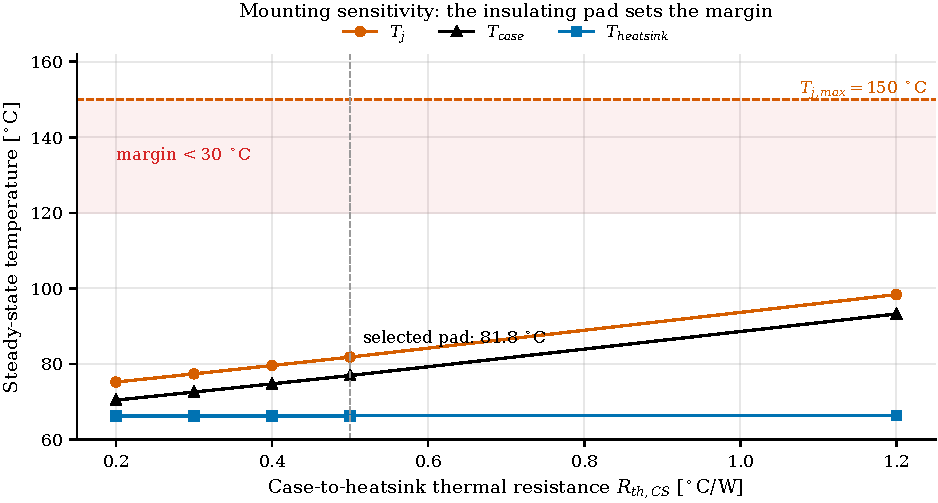
\includegraphics[width=\textwidth]{plecs_12_sensibilita_r_th_cs.pdf}
\caption{Junction, case and cold-plate temperatures against the pad thermal
resistance at the rated point, with the \SI{150}{\celsius} limit and the band
in which the margin falls below \SI{30}{\celsius}.}
\label{fig:rthcs}
\end{figure}

\begin{table}[htbp]
\centering
\caption{Sensitivity to the insulating pad at the rated point. Each row is a
separate solution of the loss--temperature loop, not an extrapolation of the
first.}
\label{tab:rthcs}
\begin{tabular}{lrrrr}
\toprule
$\Rthcs$ & $P_\mathrm{tot}$ & $\Tcase$ & $\Tj$ & Margin \\
\midrule
\SI{0.20}{\celsius\per\watt} & \SI{125.53}{\watt} & \SI{70.44}{\celsius} & \SI{75.22}{\celsius} & \SI{74.78}{\celsius} \\
\SI{0.30}{\celsius\per\watt} & \SI{126.35}{\watt} & \SI{72.58}{\celsius} & \SI{77.40}{\celsius} & \SI{72.60}{\celsius} \\
\SI{0.40}{\celsius\per\watt} & \SI{127.22}{\watt} & \SI{74.75}{\celsius} & \SI{79.60}{\celsius} & \SI{70.40}{\celsius} \\
\textbf{\SI{0.50}{\celsius\per\watt}} & \textbf{\SI{128.09}{\watt}} & \textbf{\SI{76.96}{\celsius}} & \textbf{\SI{81.84}{\celsius}} & \textbf{\SI{68.16}{\celsius}} \\
\SI{1.20}{\celsius\per\watt} & \SI{134.61}{\watt} & \SI{93.27}{\celsius} & \SI{98.40}{\celsius} & \SI{51.60}{\celsius} \\
\bottomrule
\end{tabular}
\end{table}

At the rated point the pad hardly matters: even the worst silicone pad
leaves \SI{51.6}{\celsius} of margin. The locked rotor bounds the pad. There, one device carries almost
three times the rated-point loss per device, and every tenth of a
\si{\celsius\per\watt} costs about \SI{7}{\celsius}
(\cref{sec:lockedrotor}). C1 is met up to
$\Rthcs = \SI{0.62}{\celsius\per\watt}$ with the coolant at
\SI{65}{\celsius}.

A ceramic pad (alumina or aluminium nitride) is therefore selected, with
\SI{0.50}{\celsius\per\watt} taken as a prudent class value and
\SI{0.62}{\celsius\per\watt} written into the mounting specification as
the value not to be exceeded, torque included. A filled silicone pad, at
\SI{0.5}{}--\SI{1.2}{\celsius\per\watt}, is no longer acceptable: it would
pass the rated point and fail the stalled motor. Mounting without
insulation is not an option, because the tab of the TO-247 is the drain and
would put \SI{800}{\volt} on a chassis-referenced cold plate.

The ideal plate overstates what a real rail does, and \cref{sec:cooling}
replaces it: on the rail as drawn, C1 holds only up to
\SI{0.50}{\celsius\per\watt}, which becomes the mounting limit, and the
pad adopted is aluminium nitride with a phase-change interface material, at
a design value of \SI{0.18}{\celsius\per\watt}.

\section{Locked rotor}
\label{sec:lockedrotor}

At zero output frequency the symmetry of \cref{eq:thermal-chain} is gone.
The modulator holds the phase angle at which phase~1 is at its peak: phase~1
carries the full \SI{42.4}{\ampere} as direct current, phases 2 and 3 carry
\SI{-21.2}{\ampere} each. In phase~1 the high-side device is the active
switch: it conducts for \SI{53}{\percent} of each switching period and
hard-switches \SI{42.4}{\ampere} at \SI{20}{\kilo\hertz}, while the
low-side device conducts the remaining time as a synchronous rectifier and
switches at nearly zero voltage. That
high-side device is the hottest in the converter, and it is the one C1 is
written for.

The case is simulated on the same model, with the output frequency set to
zero and the modulation amplitude re-trimmed until the phase current is
\SI{42.4}{\ampere} (\SI{26.8}{\volt} are enough, since a stalled machine
presents only its stator resistance). The thermal boundary is applied per
device: the hottest device sees the common cold plate, heated by the total
loss, plus its \emph{own} loss through the pad, not the average.

\begin{table}[htbp]
\centering
\caption{Locked rotor on the final design ($R_g = \SI{5}{}/\SI{12.5}{\ohm}$,
dead time \SI{260}{\nano\second}, $\Rthcs = \SI{0.5}{\celsius\per\watt}$),
hottest device.}
\label{tab:lockedrotor}
\begin{tabular}{lrr}
\toprule
Coolant & \SI{65}{\celsius} & \SI{70}{\celsius} \\
\midrule
Phase current (DC)          & \SI{42.43}{\ampere} & \SI{42.43}{\ampere} \\
Loss, hottest device        & \SI{61.25}{\watt}  & \SI{62.29}{\watt} \\
Loss, converter             & \SI{140.97}{\watt} & \SI{143.17}{\watt} \\
Case temperature            & \SI{97.04}{\celsius} & \SI{102.58}{\celsius} \\
\textbf{Junction temperature} & \textbf{\SI{111.05}{\celsius}} & \textbf{\SI{116.82}{\celsius}} \\
Margin to C1 (\SI{120}{\celsius}) & \SI{8.95}{\celsius} & \SI{3.18}{\celsius} \\
Margin to the \SI{150}{\celsius} limit & \SI{38.95}{\celsius} & \SI{33.18}{\celsius} \\
\bottomrule
\end{tabular}
\end{table}

The hottest device dissipates \SI{61.3}{\watt}, 2.9 times its share at the
rated point, while the converter as a whole dissipates only
\SI{10}{\percent} more. The loss is concentrated in one device, and a better
cold plate alone cannot fix that, because the heat has to cross the pad and
the die of a single device. The cold plate is at \SI{66.4}{\celsius}; the
\SI{45}{\celsius} between it and the junction are spent entirely in
$\Rthcs$ and $\Rthjc$.

Three sensitivities complete the picture:
%
\begin{itemize}
  \item Coolant temperature: \SI{+5}{\celsius} at the inlet gives
        \SI{+5.8}{\celsius} at the junction: slightly more than one to one,
        through the loop gain. C1 holds at \SI{70}{\celsius} with
        \SI{3.2}{\celsius} to spare (\cref{app:assumptions}, A.9).
  \item Pad: from \SI{0.5}{} to \SI{0.6}{} and
        \SI{0.7}{\celsius\per\watt} the junction rises to \SI{118.3}{} and
        \SI{125.8}{\celsius}; C1 is lost beyond
        \SI{0.62}{\celsius\per\watt}.
  \item Turn-off gate resistance: raising it from \SI{12.5}{} to
        \SI{15}{\ohm}, which a longer loop than \SI{20}{\nano\henry} would
        demand, costs \SI{2.0}{\celsius} (computed on the previous model
        version, with \SI{160}{\nano\second} of dead time; at \SI{12.5}{\ohm}
        the two versions agree within \SI{0.1}{\celsius}).
\end{itemize}

The die and the pad settle in well under a second; the cold plate needs
tens of seconds, but its share of the rise is only \SI{1.4}{\celsius}.
Holding a vehicle on a slope lasts longer than the former, so the steady
state is the correct criterion, and a conservative one.

\subsection{Where the loss of the hottest device comes from}
\label{sec:lrdpwm}

Splitting the \SI{61.25}{\watt} of the hottest device, by running the same
case with conduction and switching losses enabled one at a time, gives
\SI{21.2}{\watt} of conduction and \SI{40.0}{\watt} of switching. At locked
rotor, as at the rated point, switching dominates: the device hard-switches
\SI{42.4}{\ampere} twenty thousand times a second through the
\SI{12.5}{\ohm} that C2 imposes. The opposite device of the same leg
conducts for the rest of the period and carries only \SI{18.4}{\watt}.

That split is what makes discontinuous modulation interesting here, and
also what limits it. Clamping phase~1 to the positive rail (DPWM-MAX) stops
its switching, but it does not remove the current: the high-side device now
conducts for the whole period instead of \SI{53}{\percent} of it.

\begin{table}[htbp]
\centering
\caption{Locked rotor with three zero sequences, coolant \SI{65}{\celsius},
$\Rthcs = \SI{0.5}{\celsius\per\watt}$, same model and thermal loop as
\cref{tab:lockedrotor}; hottest device A1 in all three. DPWM-MAX clamps
phase~1 to the positive rail, DPWM-MIN phases 2 and 3 to the negative one.
The clamp is verified by the switching loss of the clamped device, zero.}
\label{tab:lrdpwm}
\small
\begin{tabular}{lrrrrr}
\toprule
Zero sequence & Conduction & Switching & Total & $\Tj$ & Converter \\
\midrule
\textbf{SVPWM (adopted)} & \SI{21.2}{\watt} & \SI{40.0}{\watt} & \SI{61.3}{\watt} & \textbf{\SI{111.1}{\celsius}} & \SI{141.0}{\watt} \\
DPWM-MAX & \SI{38.3}{\watt} & 0 & \SI{38.3}{\watt} & \textbf{\SI{93.9}{\celsius}} & \SI{96.0}{\watt} \\
DPWM-MIN & \SI{1.5}{\watt} & \SI{38.6}{\watt} & \SI{40.1}{\watt} & \SI{95.2}{\celsius} & \SI{95.9}{\watt} \\
\bottomrule
\end{tabular}
\end{table}

DPWM-MAX lowers the hottest junction by \SI{17.2}{\celsius}, to
\SI{93.9}{\celsius}, and the converter loss by a third. It is less than
removing the \SI{40}{\watt} of switching would suggest, because
\SI{17}{\watt} of conduction move onto the same device: the net saving on
it is \SI{23}{\watt}, not \SI{40}{\watt}. DPWM-MIN clamps the other two
phases instead; phase~1 keeps switching at a duty of \SI{5}{\percent}, and
the two devices of its leg end at \SI{95.2}{} and \SI{92.9}{\celsius}. It
is nearly as good, and either would serve. How this margin is used, as a
recommendation to the controller and not as a basis for sizing, is stated in
\cref{tab:sysassume}.

\begin{finding}{Discontinuous modulation would not have saved the \SI{40}{\milli\ohm} device}
If modulation could have kept the first device inside C1, the device change
was avoidable. The same three cases, run on the \SI{40}{\milli\ohm} devices
at their datasheet gate resistance of \SI{2.5}{\ohm}, show that it could
not:
%
\begin{center}
\small
\begin{tabular}{lrrrr}
\toprule
 & SVPWM & DPWM-MAX & DPWM-MIN & Best offset$^\ast$ \\
\midrule
C3M0040120K & \SI{140.8}{\celsius} & \SI{192.0}{\celsius} & \SI{176.2}{\celsius} & \SI{125.4}{\celsius} \\
E3M0040120K & \SI{142.3}{\celsius} & \SI{190.7}{\celsius} & \SI{174.4}{\celsius} & \SI{125.3}{\celsius} \\
\bottomrule
\multicolumn{5}{l}{\footnotesize $^\ast$ common-mode offset that balances the two devices of the leg ($d_1 \approx 0.41$).}
\end{tabular}
\end{center}
%
Where conduction dominates, as it does with \SI{40}{\milli\ohm} (\SI{61}{}
of \SI{77}{\watt}), clamping makes things worse: it concentrates the
conduction of the whole phase on one die, \SI{130}{\watt} of it. The best
that a zero sequence can do is to share that conduction evenly between the
two devices of the leg, and it stops at \SI{125}{\celsius}, still outside
C1, at a gate resistance C2 does not allow. Modulation could not have
avoided the device change, and C4 would have forced it anyway: the
C3M0040120K is not automotive.
\end{finding}

\section{The simultaneous worst case}
\label{sec:worstcase}

C1 leaves \SI{30}{\celsius} between \SI{120}{} and \SI{150}{\celsius} for
four tolerances: maximum $\Rdson$, maximum $\Rthjc$, the coolant at
\SI{70}{\celsius} and the pad at $+\SI{20}{\percent}$
(\cref{tab:criteria}). Taken one at a time they are small; the criterion
is only proven if they are taken together, with the loop between loss and
temperature closed, because each one raises the temperature that raises the
others.

\begin{table}[htbp]
\centering
\caption{Locked rotor, hottest device: the four tolerances one at a time and
together. Maximum $\Rdson$ is taken as the typical curve scaled by the
\num{22}/\num{16} ratio the datasheet gives at \SI{25}{\celsius}.}
\label{tab:worstcase}
\begin{tabular}{lrr}
\toprule
Case & $\Tj$ & Increase \\
\midrule
Nominal: \SI{65}{\celsius}, typical $\Rthjc$, pad \SI{0.50}{\celsius\per\watt} & \SI{111.1}{\celsius} & --- \\
Coolant \SI{70}{\celsius} & \SI{116.9}{\celsius} & $+\SI{5.8}{\celsius}$ \\
$\Rthjc = \SI{0.31}{\celsius\per\watt}$ (datasheet maximum) & \SI{117.0}{\celsius} & $+\SI{5.9}{\celsius}$ \\
Pad $+\SI{20}{\percent}$, \SI{0.60}{\celsius\per\watt} & \SI{118.3}{\celsius} & $+\SI{7.2}{\celsius}$ \\
Maximum $\Rdson$ & \SI{118.2}{\celsius} & $+\SI{7.1}{\celsius}$ \\
\midrule
Sum of the four & & $+\SI{26.0}{\celsius}$ \\
\textbf{All four together, loop closed} & \textbf{\SI{140.5}{\celsius}} & $\mathbf{+\SI{29.4}{\celsius}}$ \\
Same, pad at the mounting limit \SI{0.62}{\celsius\per\watt} & \SI{142.4}{\celsius} & $+\SI{31.3}{\celsius}$ \\
Same, with DPWM-MAX & \SI{126.4}{\celsius} & $+\SI{15.3}{\celsius}$ \\
\bottomrule
\end{tabular}
\end{table}

All four together cost \SI{29.4}{\celsius} against the
\SI{30}{\celsius} allowed: the junction reaches \SI{140.5}{\celsius},
\SI{9.5}{\celsius} inside the \SI{150}{\celsius} limit. This is the only
demonstration that C1 does the work it was written for, and it does. Two
lessons come with it. The a~priori split of the allowance was wrong item by item:
maximum $\Rdson$ costs \SI{7}{\celsius}, not the \SIrange{10}{13}{} assumed,
and the pad costs \SI{7}{\celsius}, not \SI{5}{}. And the interaction is not
negligible: the four together cost \SI{3.4}{\celsius} more than their sum,
the loss--temperature loop acting on a larger loss. With the pad
at its mounting limit instead of $+\SI{20}{\percent}$, the margin to
\SI{150}{\celsius} is \SI{7.6}{\celsius}.

The table comes from the analytical model of the locked rotor, which on
the nominal case reproduces the circuit model to \SI{0.1}{\celsius}
(\SI{111.1}{} against \SI{111.07}{\celsius}), because maximum $\Rdson$
would need a second copy of the vendor description. The three tolerances
that the circuit model can take directly were run there as a check: coolant
at \SI{70}{\celsius}, $\Rthjc$ at its maximum (added in series to the pad,
which is exact in steady state) and the pad at \SI{0.62}{\celsius\per\watt}
give \SI{131.9}{\celsius} in the circuit model against
\SI{132.1}{\celsius} analytically, and the pad at its limit alone
\SI{119.7}{} against \SI{119.8}{\celsius}: the analytical model holds away
from the nominal case too.

\section{From a plate resistance to a cooling solution}
\label{sec:cooling}

Every temperature so far has used one number for the whole heat sink,
$\Rthha = \SI{0.01}{\celsius\per\watt}$, a plate at the same temperature
everywhere (\cref{app:assumptions}, A.11). \Cref{sec:mechanics} then drew
the real part: a \SI{374}{\milli\metre} aluminium rail with seven TO-247
clamped along one face. This section answers three questions with one
model: what the rail as drawn achieves, whether a classic air heat
sink could replace it (preferable whenever it suffices, since it needs no
coolant loop), and which of the cooling routes open to a discrete inverter
is the best one for this design.

\paragraph{Model.} Finite-volume conduction in the rail (\SI{1}{\milli\metre}
cells across the section, \SI{2}{\milli\metre} along it), one heat source per
device spread over its contact area on the rail face, and the fluid as a row
of nodes along the rail heated by what it receives. Liquid: 50/50
water--glycol at \SI{65}{\celsius} (\cref{tab:sysassume}), Gnielinski correlation in the
channels~\cite{gnielinski}. Air: inlet at \SI{50}{\celsius}, the maximum
ambient of the specification; plate fins with the Teertstra--Yovanovich--Culham
correlation~\cite{teertstra} and the Muzychka--Yovanovich pressure
drop~\cite{muzychka}, operating point on the curve of a \SI{60}{\milli\metre}
\SI{12}{\volt} fan~\cite{delta_pfb0612}; natural convection with
Bar-Cohen and Rohsenow~\cite{barcohen}. The loss of each device comes from
the analytical locked-rotor model, which reproduces the circuit model within
\SI{0.1}{\celsius} (\cref{sec:worstcase}); the loop between losses and
temperatures is closed device by device, and the peak phase is moved to each
of the three legs, because the fluid warms along the rail. Two checks: the
heat carried away by the fluid equals the injected power to the milliwatt,
and halving the cell size moves the contact temperatures by at most
\SI{0.7}{\celsius}.

\subsection{The rail as drawn, and what air can do with the same pad}

\begin{table}[htbp]
\centering
\caption{Hottest junction with the pad of the rest of this chapter
($\Rthcs = \SI{0.50}{\celsius\per\watt}$). $R_\mathrm{eq}$ is the plate
resistance that, in the model of \cref{eq:thermal-chain}, would give the same
junction temperature. Worst case: the four tolerances of
\cref{sec:worstcase} together, the coolant at \SI{70}{\celsius}, the air at its \SI{50}{\celsius} maximum.}
\label{tab:cooling}
\small
\begin{tabular}{lrrrr}
\toprule
 & $R_\mathrm{eq}$ & Locked rotor & Worst case & Rated point \\
Cooling & [\si{\celsius\per\watt}] & [\si{\celsius}] & [\si{\celsius}] & [\si{\celsius}] \\
\midrule
Ideal plate (\cref{tab:lockedrotor}) & 0.010 & 111.1 & 140.5 & 81.8 \\
Rail as drawn, two channels, \SI{6}{\litre\per\minute} & 0.118 & 128.7 & 164.7 & 87.8 \\
Same, \SI{10}{\litre\per\minute} & 0.097 & 125.3 & 159.9 & 86.2 \\
\textbf{Six-port rail, \SI{10}{\litre\per\minute}} & \textbf{0.069} & \textbf{120.6} & \textbf{153.4} & \textbf{84.3} \\
Best forced-air sink, two fans & 0.204 & 124.9 & 157.7 & 81.6 \\
Natural convection & --- & 188 & --- & --- \\
\bottomrule
\end{tabular}
\end{table}

\begin{finding}{The ideal plate hid the spreading resistance of the real rail}
Drawn as \cref{sec:mechanics} drew it, with two \SI{8}{}$\times$\SI{8}{\milli\metre}
channels and \SI{6}{\litre\per\minute}, the rail puts the hottest junction at
\SI{128.7}{\celsius} at locked rotor, beyond C1, and the simultaneous worst
case at \SI{164.7}{\celsius}, beyond the \SI{150}{\celsius} limit. Its
equivalent resistance is twelve times the assumed plate. The cause is local:
under each tab the heat flux is about \SI{20}{\watt\per\centi\metre\squared},
and with a channel coefficient of a few \si{\kilo\watt\per\metre\squared\per\kelvin}
it must spread through the metal before the coolant can take it. A single
plate resistance cannot see spreading, and spreading is what dominates:
raising or lowering the channel coefficient by \SI{20}{\percent} moves the
junction by only \SI{0.8}{\celsius}. More flow helps little for the same
reason (\SI{125.3}{\celsius} at \SI{10}{\litre\per\minute}).
\end{finding}

The rail that the rest of this design adopts keeps solid metal where the
heat spreads and puts the coolant close behind it: an extrusion with six
ports of \SI{10}{}$\times$\SI{2}{\milli\metre}, a \SI{2}{\milli\metre} wall
towards the tabs and \SI{1}{\milli\metre} webs \emph{perpendicular} to the
face, which act as fins carrying the heat into the depth of the rail, at
\SI{10}{\litre\per\minute} and \SI{4.7}{\kilo\pascal} of pressure drop. The
first multiport attempt stacked its ports \emph{parallel} to the face and
came out worse than the two plain channels: it hollowed out exactly the
metal that spreads the flux; the second left the lowest port without a floor
where the lip ends, which the section drawing showed and the thermal model
could not. With the prudent pad even this rail falls short: C1 is
missed by \SI{0.6}{\celsius} and the worst case exceeds \SI{150}{\celsius}
by \SI{3.4}{\celsius} (\cref{fig:coolmaps}). The rail has been taken close to
what it can give; the next subsection finds where the rest of the
temperature is spent.

Forced air, given its best chance (fins attached directly behind the tabs
rather than on top of the rail, base \SI{20}{\milli\metre}, fins
\SI{87}{\milli\metre} tall and up to \SI{80}{\milli\metre} deep over the low
components, two fans), misses C1 by \SI{4.9}{\celsius} and the worst case by
\SI{7.7}{\celsius} (\cref{fig:coolair}). Natural convection is out of the
question.

\begin{figure}[htbp]
\centering
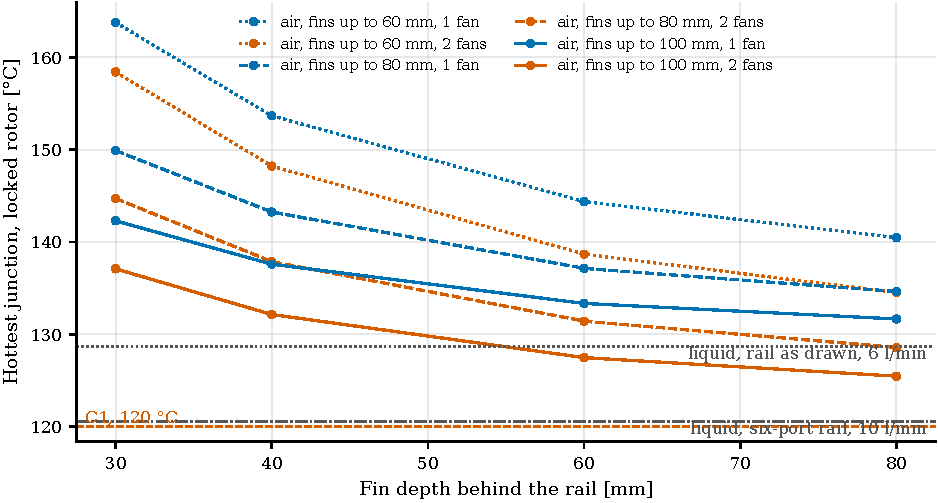
\includegraphics[width=\textwidth]{termica_raffreddamento_aria_liquido.pdf}
\caption{Forced air at \SI{50}{\celsius}: hottest junction at locked rotor
against the depth of fins attached behind the rail (\SI{20}{\milli\metre}
base, fins up to \SI{60}{}, \SI{80}{} or \SI{100}{\milli\metre} above the
board, one or two fans), with the two liquid rails for comparison;
pad \SI{0.50}{\celsius\per\watt}.}
\label{fig:coolair}
\end{figure}

\begin{figure}[htbp]
\centering
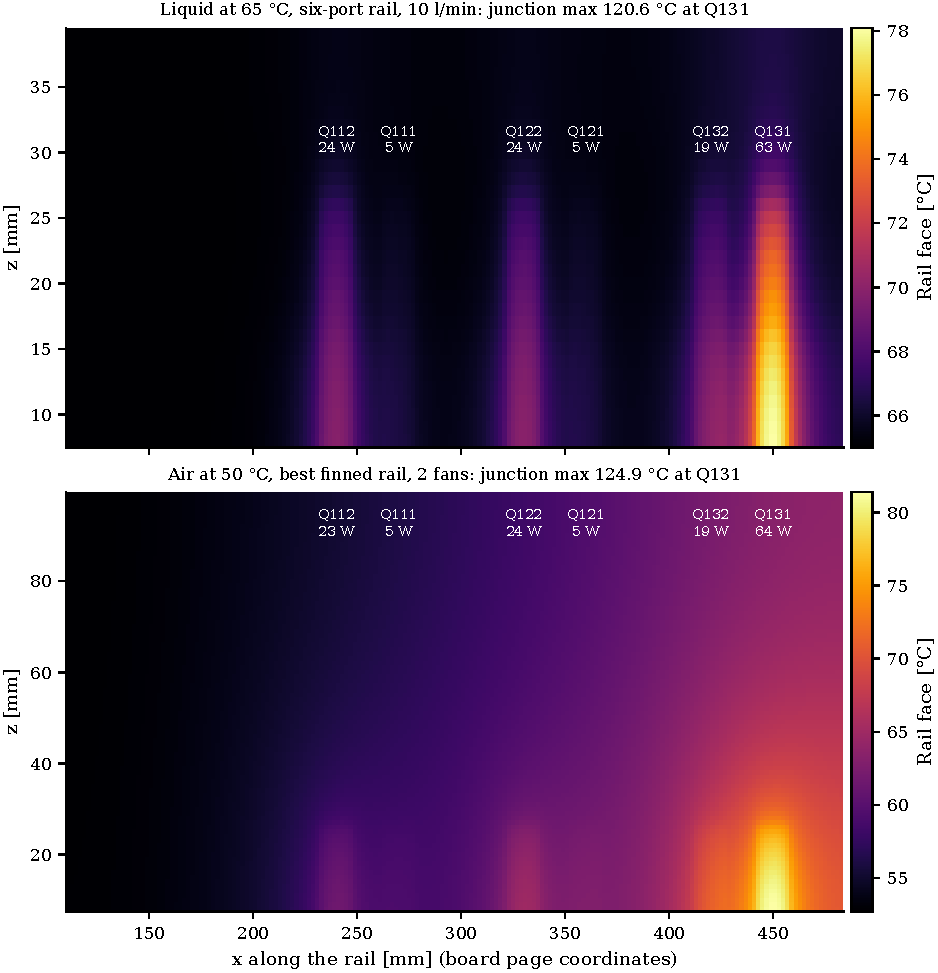
\includegraphics[width=\textwidth]{termica_raffreddamento_mappe.pdf}
\caption{Rail face temperature at locked rotor, peak current in leg~3.
Top: six-port liquid rail; the hottest strip is the lower part of the tab,
on the thin lip, farthest from the ports. Bottom: best forced-air sink; the
air warms along the rail.}
\label{fig:coolmaps}
\end{figure}

\subsection{The alternatives, on the same rail}
\label{sec:coolalt}

Between the die and the coolant there are four resistances: the die to the
case, the insulation, the spreading in the rail, the convection. At locked
rotor, on the six-port rail, the hottest device spends
\SI{14.4}{\celsius} in $\Rthjc$, \SI{31.6}{\celsius} in the pad and
\SI{9.6}{\celsius} between the rail face and the coolant. The pad is the
bottleneck, and it is the cheapest part to change. The pad itself
is a ceramic between two interfaces,
%
\begin{equation}
  \Rthcs = \frac{t_\mathrm{cer}}{k_\mathrm{cer} A} + \frac{2\,r_\mathrm{int}}{A},
\end{equation}
%
with $A = \SI{3.0}{\centi\metre\squared}$ for the tab. The
\SI{0.50}{\celsius\per\watt} of this chapter, with
\SI{0.63}{\milli\metre} alumina ($k = \SI{24}{\watt\per\metre\per\kelvin}$,
\SI{0.09}{\celsius\per\watt}), implies about
\SI{0.6}{\kelvin\centi\metre\squared\per\watt} per interface: a prudent
grease joint. A phase-change interface material under a specified clip
force reaches \SI{0.25}{\kelvin\centi\metre\squared\per\watt}, and aluminium
nitride ($k = \SI{170}{\watt\per\metre\per\kelvin}$) removes most of the
ceramic term. \Cref{tab:coolalt} runs every route on the same rail and loss
model.

\begin{table}[htbp]
\centering
\caption{Cooling alternatives on the six-port rail at \SI{10}{\litre\per\minute}
and \SI{65}{\celsius} (forced air at \SI{50}{\celsius} where stated). Worst
case: maximum $\Rthjc$, pad $+\SI{20}{\percent}$, maximum $\Rdson$, coolant
at \SI{70}{\celsius}, air at \SI{50}{\celsius}.}
\label{tab:coolalt}
\small
\begin{tabular}{lrrrr}
\toprule
 & $\Rthcs$ & Locked rotor & Worst case & With DPWM \\
Route (TO-247-4 unless stated) & [\si{\celsius\per\watt}] & [\si{\celsius}] & [\si{\celsius}] & [\si{\celsius}] \\
\midrule
Alumina, prudent value (as above) & 0.50 & 120.6 & 153.4 & 99.3 \\
Alumina + phase-change interface & 0.25 & 102.9 & 125.4 & 88.6 \\
\textbf{AlN + phase-change interface} & \textbf{0.18} & \textbf{97.9} & \textbf{117.8} & \textbf{85.6} \\
Copper spreader \SI{25\times 28}{\milli\metre} + AlN & 0.16 & 92.6 & 110.9 & 82.3 \\
Internally isolated, no external pad$^a$ & 0.08 & 98.3 & 116.7 & 85.8 \\
Forced air, one fan, AlN + phase change$^b$ & 0.18 & 108.3 & 129.1 & 85.0 \\
Top-side-cooled Q-DPAK, gap pad$^c$ & 0.61 & 139.4 & 179.9 & 110.3 \\
\bottomrule
\multicolumn{5}{l}{\footnotesize $^a$ internal ceramic counted as \SI{+0.10}{\celsius\per\watt} on $\Rthjc$; grease only outside.} \\
\multicolumn{5}{l}{\footnotesize $^b$ fins behind the rail, \SI{20}{\milli\metre} base, \SI{87\times 60}{\milli\metre} fins; coarse mesh.} \\
\multicolumn{5}{l}{\footnotesize $^c$ AIMCQ120R020M1T; $\Rthjc \approx \SI{0.26}{\celsius\per\watt}$ from its power rating; losses of the \device{} assumed.}
\end{tabular}
\end{table}

Route by route:
%
\begin{itemize}
  \item The interface decides more than the ceramic. Keeping
        alumina and changing only the interface material and the clamping
        gains \SI{17.7}{\celsius}; aluminium nitride adds \SI{5}{\celsius}
        more. The board does not change, the cost is a few euros, and the
        value becomes a mounting specification, confirmed by measuring the
        mounted pad.
  \item A copper spreader at drain potential between tab and pad
        spreads the flux over \SI{7}{\centi\metre\squared} and gains another
        \SI{5}{\celsius}. It is not worth it here: a second clamped joint,
        and spreaders of opposite potentials \SI{5}{\milli\metre} apart where the
        creepage asks for \SI{4.5}{}.
  \item Internally isolated TO-247-4 packages put the ceramic
        inside, under the die (Littelfuse ISO247, Navitas UHV-TO-247-4-ISO
        with AlN, Luminus ISOMOS~\cite{littelfuse_iso247,navitas_uhviso}):
        same footprint, no external pad, vendor claims of up to
        \SIrange{60}{64}{\percent} lower junction-to-heat-sink resistance. In
        this model they match the AlN pad, with one interface and one
        assembly step less. None is offered at
        \SI{16}{\milli\ohm} with AEC-Q101 qualification today, so it fails
        C4 and stays a production watch item.
  \item Top-side-cooled packages (Q-DPAK, TOLT, HU3PAK, U2) are now
        available in the automotive \SI{1200}{\volt} range down to
        \SI{19}{\milli\ohm}~\cite{infineon_aimcq}. Their top pad is the
        drain, about half the area of a TO-247 tab, and needs an insulating
        gap pad: thermally worse here, by \SI{19}{\celsius}. Their strengths are
        automated assembly and loop inductance, and adopting them would
        mean a new board.
  \item A plane on the bottom of the board does not help a through-hole
        device: only the drain lead is joined to the tab, and at
        \SI{18}{\celsius\per\watt} it carries at most \SI{4}{\percent} of the
        heat. A bottom-cooled SMD package needs eighty filled vias and an
        insulator under its drain pad, \SI{1.9}{\celsius\per\watt}, ten times
        the AlN pad.
  \item Classic heat sinks work only with the better pad and a fan,
        and then they work: one fan, \SI{108.3}{\celsius} at locked rotor and
        \SI{129.1}{\celsius} in the worst case. They lose on other
        grounds. The fins sit over the high-voltage board, so the
        enclosure must breathe outside air across it and the uncoated areas
        (terminals, connectors, test points) leave pollution degree~2; the
        fan is a wear part whose failure at standstill takes the junction
        towards the natural-convection figure within seconds, so it would
        need tachometer supervision and immediate derating; and the sink is
        about ten times the volume of the rail. The vehicle already has a
        liquid loop (\cref{tab:sysassume}).
\end{itemize}

\begin{finding}{Adopted cooling: six-port rail and aluminium nitride pad}
The adopted solution is the six-port liquid rail at \SI{10}{\litre\per\minute},
with \SI{0.63}{\milli\metre} aluminium nitride and a phase-change interface
on both faces under a specified clip force, $\Rthcs \le \SI{0.18}{\celsius\per\watt}$
as design value. The hottest junction at locked rotor falls from
\SI{120.6}{} to \SI{97.9}{\celsius}, the simultaneous worst case from
\SI{153.4}{} to \SI{117.8}{\celsius}: \SI{32.2}{\celsius} from the
\SI{150}{\celsius} limit, without touching the frozen board. The pad value
not to be exceeded at assembly becomes \SI{0.50}{\celsius\per\watt}, at which
C1 is still met on the real rail. The
device-level results of this chapter, computed on the ideal plate with the
prudent pad, remain a valid comparison between candidates; the absolute
temperatures of the design are those of \cref{tab:coolalt}.
\end{finding}

\section{Thermal transient}

The thermal time constant of the cold plate is of the order of seconds,
while the solver step is about \SI{1}{\micro\second} at \SI{20}{\kilo\hertz},
so a short window is simulated and an exponential identified from it. The
heat capacity of \SI{1000}{\joule\per\kelvin} is estimated from geometry: a
\SI{200}{}$\times$\SI{150}{}$\times$\SI{12}{\milli\metre} aluminium plate with
\SI{15}{\percent} of its volume taken by channels gives
\SI{744}{\joule\per\kelvin} of metal, \SI{204}{\joule\per\kelvin} of retained
coolant and roughly \SI{90}{\joule\per\kelvin} of fittings. The
identification gives $\tau = \SI{10.20}{\second}$ against
\SI{10.00}{\second} expected, and the temperature rise agrees with
$P_\mathrm{tot}\Rthha$ within \SI{1.6}{\percent}. The heat capacity affects
only the transient: all eleven steady-state operating points reproduce
bit-for-bit with the value doubled.

\section{The other components: temperature and life}
\label{sec:complife}

This section checks the other components of the power stage (the DC-link
films, the commutation ceramics and the shunts) against their manufacturers'
limits. Two assumptions frame it: the air inside the enclosure is
\SI{70}{\celsius} in normal operation and \SI{85}{\celsius} in a hot case,
since the liquid loop at \SI{65}{\celsius} sets the interior rather than the
\SI{50}{\celsius} outside; and the mission is \SI{8000}{\hour} of operation
with the bus energised, the usual order for fifteen years of a passenger car.

\begin{table}[htbp]
\centering
\caption{Stress, temperature and margin of the power-stage components that
carry high voltage or ripple current. Air inside the enclosure \SI{70}{\celsius},
hot case \SI{85}{\celsius}; power copper up to \SI{30}{\kelvin} above it
(\cref{tab:widths}).}
\label{tab:complife}
\small
\begin{tabularx}{\textwidth}{lllY}
\toprule
Component & Stress & Temperature & Margin \\
\midrule
Film C101, \SI{140}{\micro\farad} & \SI{13.7}{} of \SI{43.5}{\ampere}, \SI{0.37}{\watt} & hotspot $+\SI{1.5}{\kelvin}$ & \SI{63000}{\hour} at \SI{900}{\volt}, \SI{85}{\celsius} \\
Film C102, \SI{60}{\micro\farad} & \SI{5.9}{} of \SI{40}{\ampere}, \SI{0.09}{\watt} & hotspot $+\SI{0.6}{\kelvin}$ & as C101, slightly better \\
KC-LINK, $12\times\SI{47}{\nano\farad}$ & \SIrange{1.0}{2.0}{\ampere} each, \SI{2}{\mega\hertz} & a few tenths of a kelvin & \SI{12}{\ampere} allowed; C0G does not age \\
Shunts, \SI{0.5}{\milli\ohm} & \SI{0.45}{}/\SI{0.90}{\watt} rated/stalled & terminals \SIrange{100}{115}{\celsius} & \SIrange{5.0}{6.3}{\watt} allowed there \\
\bottomrule
\end{tabularx}
\end{table}

\paragraph{The film capacitors.} Their life is the only one in the table
that is consumed. The manufacturer gives it as a family of lines, life
against the ratio of operating to rated voltage, at
\SI{70}{}, \SI{85}{} and \SI{105}{\celsius}~\cite{vishay_mkp1848}; read from
the graph and interpolated in temperature, it gives \SI{94000}{\hour} at
rated voltage and \SI{70}{\celsius}, consistent with the
\SI{100000}{\hour} the datasheet declares, which is the check of the
reading. The self-heating is small, so life is a function of the air around
the capacitor (\cref{fig:filmlife}): the mission is met at \SI{900}{\volt}
continuous up to \SI{99.7}{\celsius} of air. The \SI{1100}{\volt} class
chosen for the voltage derating (\cref{sec:dclink}) is what buys this: at
the same temperature a \SI{900}{\volt} part would sit at its rated voltage.

\begin{figure}[htbp]
\centering
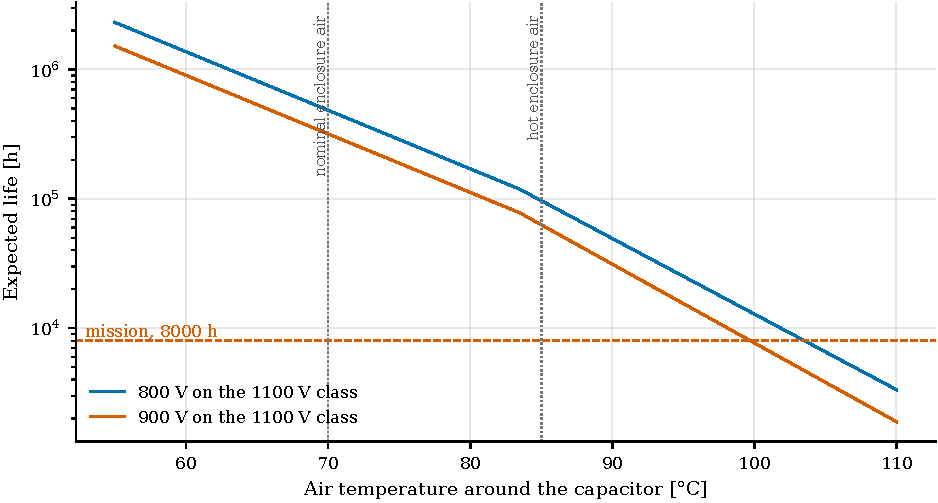
\includegraphics[width=\textwidth]{termica_componenti_vita_film.pdf}
\caption{Expected life of the DC-link film capacitors against the air
temperature around them, at the nominal and the maximum continuous bus
voltage, from the manufacturer's life curves.}
\label{fig:filmlife}
\end{figure}


\paragraph{The ceramics ring with the films.} At every switching edge the
step in bridge current is first supplied by the ceramics, then handed to
the films through their inductance, about \SI{11}{\nano\henry} with the
planes: a damped ring at
$f_0 = 1/(2\pi\sqrt{L\,C}) \approx \SI{2.0}{\mega\hertz}$ with
$C = \SI{564}{\nano\farad}$. With the energy of each ring
$\Delta I^2/(4\alpha)$, $\alpha = R/2L$, summed over six edges per switching
period, the ceramics carry \SIrange{12}{24}{\ampere} in total for a loop
resistance of \SIrange{4}{1}{\milli\ohm}: \SIrange{1}{2}{\ampere} each,
well inside their rating.

\paragraph{The shunts} dissipate a fifth of what their terminals allow even
in the hot case. What their temperature does affect is accuracy: with
\SI{100}{ppm\per\kelvin} including the copper terminals, a rise of
\SI{60}{\kelvin} above calibration is \SI{0.6}{\percent} of gain error, to be
added to the measurement budget or compensated with the cold-plate
thermistor.

\chapter{Auxiliary circuits}
\label{ch:aux}

\section{Gate drive}

\subsection{Requirements}

The peak gate current follows from the gate charge and the total gate-loop
resistance:
%
\begin{equation}
  I_{g,\mathrm{pk}} = \frac{V_\mathrm{DD} - V_\mathrm{EE}}
                           {R_{g,\mathrm{on}} + R_{G(\mathrm{int})} + R_\mathrm{drv}}
  = \frac{\SI{20}{\volt}}{\SI{5}{\ohm} + \SI{2.6}{\ohm} + \SI{2.5}{\ohm}}
  = \SI{1.98}{\ampere},
\end{equation}
%
and the average gate-drive power per channel from the gate charge:
%
\begin{equation}
  P_g = Q_g \, (V_\mathrm{DD}-V_\mathrm{EE}) \, \fsw
      = \SI{223}{\nano\coulomb} \cdot \SI{20}{\volt} \cdot \SI{20}{\kilo\hertz}
      = \SI{89.2}{\milli\watt}.
\end{equation}
%
The \SI{20}{\volt} swing is $+15$ to $-5$~V, the choice justified in
\cref{sec:negbias}.

\subsection{Driver selection}

\begin{table}[htbp]
\centering
\caption{Isolated gate driver alternatives.}
\label{tab:driver}
\small
\begin{tabularx}{\textwidth}{lYYY}
\toprule
 & \textbf{\driver{}} & Basic isolated driver & Optocoupler driver \\
\midrule
Isolation & \textbf{reinforced, \SI{2121}{\volt} DC} & basic & reinforced \\
CMTI & \textbf{\SI{150}{\volt\per\nano\second}} & \SI{50}{}--\SI{100}{\volt\per\nano\second} & \SI{25}{}--\SI{50}{\volt\per\nano\second} \\
Desaturation detection & \textbf{integrated} & external & some \\
Active Miller clamp & \textbf{integrated} & external & rare \\
Soft turn-off & \textbf{integrated} & no & no \\
Propagation delay & \SI{90}{\nano\second} & similar & \SI{150}{}--\SI{300}{\nano\second} \\
Ageing & \textbf{capacitive, stable} & --- & LED degrades \\
\bottomrule
\end{tabularx}
\end{table}

The \driver{} is selected~\cite{ti_ucc21750}; \cref{fig:gatechannel} shows
one channel as built. The decisive parameter is the
common-mode transient immunity. In the double-pulse simulation at the
overvoltage and overload thresholds (\cref{sec:kelvin}) the switching node
moves at \SI{31}{\volt\per\nano\second} between \SI{10}{} and
\SI{90}{\percent} of the steeper edge, and at \SI{70}{\volt\per\nano\second}
over the steepest nanosecond, ringing included. A driver rated
\SI{50}{\volt\per\nano\second} would be exceeded; the
\SI{150}{\volt\per\nano\second} rating leaves a factor of 2.1 on the
steepest value.

Optocoupler-based drivers are rejected on two grounds: their propagation
delay is two to three times larger, which directly enlarges the dead-time
budget of \cref{tab:deadtime}, and the LED degrades with time and
temperature, which is a poor property in an automotive application.

\begin{figure}[htbp]
\centering
% Un canale di gate: driver isolato, resistenze separate di accensione e spegnimento, sorgente
% Kelvin, rete di desaturazione con zener, alimentazione isolata +15/-5 V.
\begin{circuitikz}[font=\footnotesize, >=Stealth]
  % driver isolato (pin disposti per non incrociare i collegamenti)
  \draw[thick, fill=fblu!6] (0,0) rectangle (3.0,5.3);
  \node[font=\footnotesize\bfseries] at (1.5,5.6) {isolated driver};
  \draw[very thick, dashed, fgrigio] (1.0,-0.25) -- (1.0,5.5);
  \node[font=\scriptsize, rotate=90, fgrigio] at (0.7,2.6) {reinforced barrier};
  \foreach \y/\t in {4.2/PWM, 3.4/enable, 2.6/fault, 1.8/ready}
    \draw[<->, fblu] (-1.0,\y) node[left]{\t} -- (0,\y);
  \foreach \y/\t in {4.9/DESAT, 3.5/OUTH, 2.7/OUTL, 1.7/COM, 1.0/VDD, 0.4/VEE}
    \node[anchor=east, font=\scriptsize] at (2.95,\y) {\t};
  % resistenze di gate separate
  \draw (3.0,3.5) to[R, l={$R_{g,\mathrm{on}}$, \SI{5}{\ohm}}] (5.6,3.5) -- (6.3,3.5) -- (6.3,3.1) coordinate (g);
  \draw (3.0,2.7) to[R, l_={$R_{g,\mathrm{off}}$, \SI{12.5}{\ohm}}] (5.6,2.7) -- (6.3,2.7) -- (g);
  \draw (g) -- (7.4,3.1) node[nmos, bodydiode, anchor=G] (Q) {};
  \draw (Q.D) -- ++(0,1.8) node[above]{drain};
  \draw (Q.S) -- ++(0,-0.9) node[below]{power source};
  % sorgente Kelvin: il ritorno del driver va al source sul die, non sul percorso di potenza
  \draw (3.0,1.7) -- ($(Q.S |- 0,1.7)+(-0.35,0)$) |- ($(Q.S)+(0,-0.3)$);
  \node[font=\scriptsize, anchor=north] at ($(Q.S |- 0,1.7)+(-1.4,0)$) {Kelvin source};
  % desaturazione: resistenza, condensatore di blanking verso COM, zener, diodo HV al drain
  \draw (3.0,4.9) to[R, l={\SI{1}{\kilo\ohm}}, -*] (4.2,4.9) coordinate (dn);
  \draw (dn) to[C, l_={$C_\mathrm{blank}$}] (4.2,6.0) node[above, font=\scriptsize]{to COM};
  \draw (dn) -- (5.0,4.9) to[zDo, l_={\SI{4.3}{\volt} zener}] (6.4,4.9)
        to[D, l_={SiC diode}, -*] ($(Q.D |- 0,4.9)$);
  % alimentazione isolata del lato secondario
  \draw[thick, fill=fverde!8] (0.2,-1.7) rectangle (3.0,-0.7);
  \node[align=center, font=\scriptsize] at (1.6,-1.2) {isolated DC/DC\\$+\SI{15}{}/-\SI{5}{\volt}$};
  \draw[->] (3.0,-0.95) -| (3.5,1.0) -- (3.0,1.0);
  \draw[->] (3.0,-1.45) -| (3.8,0.4) -- (3.0,0.4);
\end{circuitikz}

\caption{One gate-drive channel. Separate turn-on and turn-off resistors, the
driver's return to the Kelvin source rather than to the power source, the
desaturation network with the \SI{4.3}{\volt} zener of
\cref{sec:protection}, and the isolated $+\SI{15}{}/-\SI{5}{\volt}$
supply.}
\label{fig:gatechannel}
\end{figure}

\subsection{Gate resistance and negative bias}

$R_{g,\mathrm{on}} = \SI{5}{\ohm}$ and $R_{g,\mathrm{off}} = \SI{12.5}{\ohm}$,
on the two separate outputs of the driver, with footprints allowing up to
\SI{25}{\ohm}. They are the smallest values that keep the die below \SI{1080}{\volt} at \SI{950}{\volt} and \SI{60}{\ampere} with
the \SI{20}{\nano\henry} layout budget (\cref{sec:kelvin}): $R_{g,\mathrm{off}}$
is set by the turn-off of the device itself, $R_{g,\mathrm{on}}$ by the
recovery of the opposite diode, and the separate outputs are what allow the
two to differ. The first version of this design
used \SI{2.5}{\ohm} on the argument that overshoot margin is cheaper to buy
from the layout; that argument holds for margin \emph{beyond} the
criterion, not for the criterion itself.

\subsection{Negative bias: why \texorpdfstring{$-\SI{5}{\volt}$}{-5 V}}
\label{sec:negbias}

A negative off-state bias is mandatory. With the gate
held at \SI{0}{\volt}, the Miller current injected through $C_\mathrm{gd}$
during the opposite device's turn-on raises the gate voltage by
%
\begin{equation}
  \Delta V_\mathrm{GS} = C_\mathrm{gd,eff}\,\frac{\mathrm{d}v}{\mathrm{d}t}\,R
  \left[1 - \exp\!\left(-\frac{t}{R\,C_\mathrm{iss}}\right)\right].
  \label{eq:miller}
\end{equation}

The datasheet quotes $-\SI{4}{\volt}$ as the \emph{typical operating}
value, not as a limit: the absolute maximum is
$-\SI{8}{\volt}$~\cite{wolfspeed_e3m0016}. This design uses
$-\SI{5}{\volt}$, which is what the standard isolated module delivers
without an extra regulator, and which leaves \SI{3}{\volt} to the absolute
maximum.

Since \cref{eq:miller} does not depend on the bias, the extra volt
translates one-for-one into margin. The equation is evaluated with
$C_\mathrm{gd,eff} = Q_\mathrm{gd}/V_\mathrm{DS} = \SI{81}{\pico\farad}$,
$C_\mathrm{iss} = \SI{6922}{\pico\farad}$ and the turn-on slope that the
double-pulse simulation gives for the opposite device,
\SI{31.4}{\volt\per\nano\second}; the closed-form slope from the gate current
would be only \SI{14.3}{\volt\per\nano\second}, and the steeper value is the
one used. Without the clamp the off device is held through
$R_{g,\mathrm{off}} + R_{G(\mathrm{int})}$ plus the driver's sink
resistance, \SI{15.4}{\ohm}. The same case was then simulated directly, holding the off device
at \SI{-5}{\volt} through its gate resistor, and reading $V_\mathrm{GS}$ at
the die:

\begin{table}[htbp]
\centering
\caption{Margin against spurious turn-on at \SI{950}{\volt},
\SI{60}{\ampere}. $V_\mathrm{GS(th)}$ is the \SI{1.8}{\volt} minimum at
\SI{25}{\celsius}~\cite{wolfspeed_e3m0016}.}
\label{tab:miller}
\begin{tabular}{lrrr}
\toprule
Configuration & \Cref{eq:miller} & Margin & Simulated, at the die \\
\midrule
$-\SI{4}{\volt}$, no clamp   & $+\SI{4.35}{\volt}$ & $-\SI{2.55}{\volt}$ & --- \\
$-\SI{4}{\volt}$, with clamp & $+\SI{1.58}{\volt}$ & \SI{0.22}{\volt} & --- \\
$-\SI{5}{\volt}$, no clamp   & $+\SI{3.35}{\volt}$ & $-\SI{1.55}{\volt}$ & $-\SI{1.33}{\volt}$ \\
\textbf{$-\SI{5}{\volt}$, with clamp} & $\mathbf{+\SI{0.58}{\volt}}$ & \textbf{\SI{1.22}{\volt}} & $\mathbf{-\SI{2.98}{\volt}}$ \\
\bottomrule
\end{tabular}
\end{table}

The clamp is still required. The closed form is a bound, not a
prediction: it charges the whole Miller current into the external resistance
for the whole edge, and the simulation, which resolves the internal gate
network, keeps the die \SIrange{4}{5}{\volt} lower. But the bound is the
number that can be defended without trusting a model's gate network, and by
that number $-\SI{5}{\volt}$ alone fails and $-\SI{5}{\volt}$ with the clamp
passes with \SI{1.22}{\volt}. The integrated active Miller clamp removes the
dependence on $R_{g,\mathrm{off}}$ by shorting the gate through a separate
low-impedance path; with \SI{12.5}{\ohm} of $R_{g,\mathrm{off}}$ it is what
makes the margin exist.

One effect runs the other way: the body
diode forward voltage is characterised at
$V_\mathrm{GS} = -\SI{4}{\volt}$~\cite{wolfspeed_e3m0016}, so a more negative
gate raises it slightly and with it the dead-time loss of
\cref{sec:deadtime-loss}. The effect is a few hundredths of a watt, under
\SI{0.05}{\percent} of the total, but it is the reason not to go to
$-\SI{8}{\volt}$ merely because the margin allows it.

\section{Protection}
\label{sec:protection}

\subsection{Overcurrent: two mechanisms, two roles}

\begin{table}[htbp]
\centering
\caption{Protection assignment.}
\label{tab:protection}
\small
\begin{tabularx}{\textwidth}{lllY}
\toprule
Mechanism & Threshold & Response time & Covers \\
\midrule
Desaturation, with \SI{4.3}{\volt} zener & \SIrange{143}{259}{\ampere} & \SI{0.69}{}/\SI{0.83}{\micro\second}$^\ast$ & hard short, shoot-through \\
Shunt + comparator & $\approx\SI{60}{\ampere}$ & \SI{3}{}--\SI{4}{\micro\second} & overload, ground fault, stall \\
\bottomrule
\multicolumn{4}{l}{\footnotesize $^\ast$ typical/worst case, counted as $t_\mathrm{SC}$ is measured (\cref{tab:scchain}).}
\end{tabularx}
\end{table}

\begin{figure}[htbp]
\centering
% Scale di tempo: ogni protezione e' assegnata al guasto che riesce a raggiungere in tempo.
% Asse logaritmico; ogni barra va dall'inizio dell'evento al suo tempo (capitoli 7 e 8).
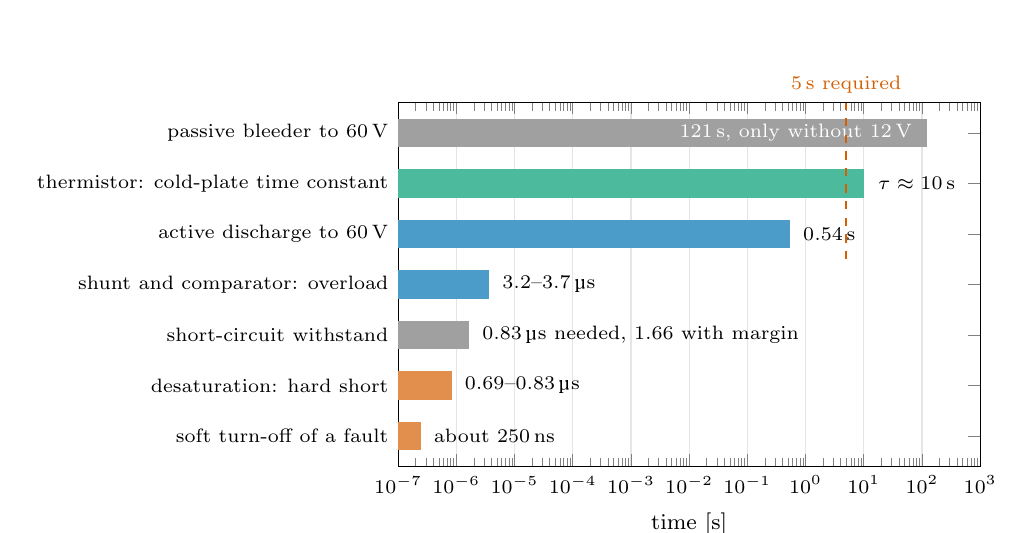
\begin{tikzpicture}
  \begin{axis}[
    width=0.74\textwidth, height=6.2cm, xmode=log, clip=false,
    xmin=1e-7, xmax=1e3, ymin=0.4, ymax=7.6,
    ytick={1,...,7},
    yticklabels={{soft turn-off of a fault}, {desaturation: hard short}, {short-circuit withstand},
                  {shunt and comparator: overload}, {active discharge to \SI{60}{\volt}},
                  {thermistor: cold-plate time constant}, {passive bleeder to \SI{60}{\volt}}},
    xlabel={time [s]}, xmajorgrids, grid style={black!10},
    tick label style={font=\scriptsize}, label style={font=\footnotesize}]
    % barre: dall'inizio dell'evento al tempo caratteristico
    \foreach \b/\r/\c in {2.5e-7/1/farancio, 0.83e-6/2/farancio, 1.66e-6/3/fgrigio, 3.7e-6/4/fblu,
                          0.54/5/fblu, 10/6/fverde, 121/7/fgrigio} {
      \edef\tmp{\noexpand\fill[\c!70] (axis cs:1e-7,\r-0.28) rectangle (axis cs:\b,\r+0.28);}\tmp
    }
    \node[font=\scriptsize, anchor=west] at (axis cs:2.8e-7,1) {about \SI{250}{\nano\second}};
    \node[font=\scriptsize, anchor=west] at (axis cs:0.95e-6,2) {\SI{0.69}{}--\SI{0.83}{\micro\second}};
    \node[font=\scriptsize, anchor=west] at (axis cs:1.9e-6,3) {\SI{0.83}{\micro\second} needed, \SI{1.66}{} with margin};
    \node[font=\scriptsize, anchor=west] at (axis cs:4.2e-6,4) {\SI{3.2}{}--\SI{3.7}{\micro\second}};
    \node[font=\scriptsize, anchor=west] at (axis cs:0.62,5) {\SI{0.54}{\second}};
    \node[font=\scriptsize, anchor=west] at (axis cs:12,6) {$\tau \approx \SI{10}{\second}$};
    \node[font=\scriptsize, anchor=east, text=white] at (axis cs:100,7) {\SI{121}{\second}, only without \SI{12}{\volt}};
    % requisito di scarica
    \draw[dashed, farancio, thick] (axis cs:5,4.5) -- (axis cs:5,7.6);
    \node[font=\scriptsize, farancio, anchor=south] at (axis cs:5,7.6) {\SI{5}{\second} required};
  \end{axis}
\end{tikzpicture}

\caption{Time scales of the protections and of the events they answer. Each layer
covers the faults it can reach in time: desaturation the hard short, inside
the withstand time; the shunt chain the overload; the thermistor the loss
of cooling; the active discharge the \SI{5}{\second} requirement, which the
passive bleeder alone misses.}
\label{fig:protecttime}
\end{figure}

\Cref{fig:protecttime} places every protection on the time scale of the
fault it answers. Desaturation detection on a SiC MOSFET is harder than on
an IGBT, and the
report should say so. The method compares the on-state drain voltage with a
threshold; an IGBT in short circuit presents several volts of
$V_\mathrm{CE(sat)}$, whereas a SiC MOSFET presents only $I\cdot\Rdson$. The
driver threshold sits at \SI{9.15}{\volt}~\cite{ti_ucc21750}; less the
blocking diode drop, the drain trips at about \SI{8.45}{\volt}.

\begin{finding}{With a \SI{16}{\milli\ohm} device, the native threshold trips beyond the pulsed rating}
$8.45 / \Rdson$ is \SI{291}{\ampere} with the die at \SI{175}{\celsius}
and \SI{528}{\ampere} at \SI{25}{\celsius}, against a pulsed drain rating of
\SI{321}{\ampere}~\cite{wolfspeed_e3m0016}. A cold device with a slowly
rising fault current (a short through a motor winding rather than across the
bridge) would reach its rating before the protection saw it. The threshold
that was comfortable with a \SI{40}{\milli\ohm} device is wrong with a
\SI{16}{\milli\ohm} one.
\end{finding}

A \SI{4.3}{\volt} zener in series with the blocking diode lowers the drain
threshold to about \SI{4.15}{\volt}: \SI{143}{\ampere} hot, \SI{259}{\ampere}
at \SI{25}{\celsius} with a typical device and \SI{189}{\ampere} with a
maximum-resistance one, all below the pulsed rating. Normal operation stays
well clear of it: at the \SI{42.4}{\ampere} rated peak a hot device shows
\SI{1.23}{\volt}, a factor of 3.4, and at the \SI{60}{\ampere} overload trip
\SI{1.74}{\volt}, a factor of 2.4. Those are typical figures. Stacking the
tolerances (the lowest detection threshold, \SI{8.5}{\volt}; a blocking
diode at \SI{0.8}{\volt}; the zener at $+\SI{5}{\percent}$; a hot device at
maximum resistance, taken as the typical hot value scaled by the
\num{22}/\num{16} ratio the datasheet gives at \SI{25}{\celsius}), the trip
point falls to \SI{3.19}{\volt} and the \SI{60}{\ampere} operating point
rises to \SI{2.39}{\volt}: a factor of 1.33. That factor, not 2.4, is what
limits any further lowering of the threshold (\cref{sec:planb}). One zener
per channel is the whole cost.

The shunt chain is deliberately \emph{not} assigned to short-circuit
protection, because it cannot reach it. The \isoamp{} alone has a
propagation delay of \SI{2.1}{\micro\second} maximum at
\SI{50}{\percent}--\SI{50}{\percent} and \SI{3.0}{\micro\second} to
\SI{90}{\percent}~\cite{ti_amc1302}, set by its sigma-delta modulator; with
the comparator and the soft turn-off the chain totals
\SI{3.2}{}--\SI{3.7}{\micro\second}. That is fine for an overload, which
develops over milliseconds, and useless against a short.

\subsection{Blanking}

The driver already provides \SI{200}{\nano\second} of leading-edge blanking
internally~\cite{ti_ucc21750}. The external capacitor adds only the
difference:
%
\begin{equation}
  t_\mathrm{add} = \frac{C_\mathrm{blank}\,V_\mathrm{DESAT}}{I_\mathrm{CHG}}
  = \frac{C_\mathrm{blank}\cdot\SI{9.15}{\volt}}{\SI{500}{\micro\ampere}} .
\end{equation}
%
With $C_\mathrm{blank} = \SI{10}{\pico\farad}$ the total is about
\SI{383}{\nano\second}, which covers
$t_\mathrm{d(on)} + t_r \approx \SI{81}{\nano\second}$ at
$R_{g,\mathrm{on}} = \SI{5}{\ohm}$~\cite{wolfspeed_e3m0016} with a wide
margin. Going
below \SI{10}{\pico\farad} is pointless: stray capacitance becomes
comparable with the component.

\subsection{Soft shutdown}

At \SI{60}{\ampere} and $R_{g,\mathrm{off}} = \SI{12.5}{\ohm}$ the die already
reaches \SI{1073.5}{\volt} (\cref{sec:kelvin}). Turning off a fault of
\SIrange{150}{260}{\ampere} through the same resistor would produce a
$\mathrm{d}i/\mathrm{d}t$ that, across the same loop, exceeds
\SI{1200}{\volt}: the protection would destroy the device it is protecting.
The driver's integrated soft turn-off pulls the gate down through a
\SI{400}{\milli\ampere} current source instead, lengthening the turn-off to
roughly \SI{250}{\nano\second} and keeping the overshoot bounded.

\subsection{Short-circuit withstand}
\label{sec:tsc}

The \device{} datasheet does not declare a short-circuit withstand
time. It is the one selection criterion the device does not demonstrate
(\cref{sec:deviceselection}), and the way to carry an unknown of this kind is
to turn it into a threshold: the value below which the protection no longer
protects.

\paragraph{The threshold.} The manufacturer measures $t_\mathrm{SC}$ from
\SI{50}{\percent} of the gate voltage at turn-on to \SI{50}{\percent} at
turn-off~\cite{wolfspeed_scan}, so the protection chain is counted the same
way, for the worst fault: a short already present at turn-on, which has to
wait out the blanking (\cref{tab:scchain}).

\begin{table}[htbp]
\centering
\caption{Desaturation chain, counted as $t_\mathrm{SC}$ is measured,
datasheet tolerances~\cite{ti_ucc21750}.}
\label{tab:scchain}
\begin{tabular}{lrr}
\toprule
Contribution & Typical & Worst case \\
\midrule
Internal leading-edge blanking & \SI{200}{\nano\second} & \SI{200}{\nano\second} \\
External blanking, $C_\mathrm{blank}V_\mathrm{DESAT}/I_\mathrm{CHG}$, \SI{10}{\pico\farad}
  & \SI{183}{\nano\second} & \SI{228}{\nano\second} \\
Detection to output low (deglitch included) & \SI{200}{\nano\second} & \SI{300}{\nano\second} \\
Soft turn-off, \SI{90}{\percent} to \SI{50}{\percent} of the gate swing & \SI{138}{\nano\second} & \SI{138}{\nano\second} \\
Less turn-on to \SI{50}{\percent} of the gate swing & $-\SI{36}{\nano\second}$ & $-\SI{36}{\nano\second}$ \\
\midrule
\textbf{Total} & \textbf{\SI{0.69}{\micro\second}} & \textbf{\SI{0.83}{\micro\second}} \\
\bottomrule
\end{tabular}
\end{table}

The design survives a short if $t_\mathrm{SC} \geq
\SI{0.83}{\micro\second}$, and has a factor of two at
\SI{1.66}{\micro\second}. The earlier figure of
\SIrange{0.65}{0.75}{\micro\second} was the typical chain; C5, fixed at
\SI{1.5}{\micro\second} before the tolerances were stacked, gives a factor
of 1.8 on the worst case.

\paragraph{What $t_\mathrm{SC}$ depends on.} During a short the device
sits in saturation with the whole bus across it, and it fails when the
energy $E_\mathrm{SC} \approx V_\mathrm{bus} I_\mathrm{sat} t$ reaches a
critical value set by the die: its area and its thermal mass, not the
circuit~\cite{wolfspeed_scan}. The circuit sets the other two factors.
$V_\mathrm{bus}$ is fixed. $I_\mathrm{sat}$ is set by the gate voltage,
roughly as $(V_\mathrm{GS} - V_\mathrm{th})^n$ with $n$ between 1 and 2.
This is where \SI{+15}{\volt} helps: it is the bottom of the range used
for SiC, where \SI{+18}{} and \SI{+20}{\volt} are common, and with
$V_\mathrm{th} = \SI{2.5}{\volt}$ the saturation current at \SI{+18}{\volt}
is \SIrange{24}{54}{\percent} higher, at \SI{+20}{\volt}
\SIrange{40}{96}{\percent} higher. For the same critical energy the
withstand time is shorter in the same proportion. A datasheet value
quoted at \SI{+18}{\volt} would be pessimistic for this design.

\paragraph{A class value.} The manufacturer has published a measurement on
the same die generation and resistance class: a \SI{16}{\milli\ohm} Gen~3
die in a half-bridge module survives \SI{2.9}{\micro\second} at
\SI{800}{\volt}, \SI{175}{\celsius} and \SI{+15}{\volt}, with a critical
energy of about \SI{1.4}{\joule}~\cite{wolfspeed_scan}. Scaled at constant
energy it becomes \SI{2.6}{\micro\second} at \SI{900}{\volt} and
\SI{2.4}{\micro\second} at \SI{950}{\volt}, 2.9 times the worst-case chain.
This is a class value, not a property of the \device{}: another
package, another die lot, an application note rather than a datasheet. It
says that the threshold is plausibly met with margin, not that it is met.
Peer-reviewed measurements on \SI{1.2}{\kilo\volt} devices show the same
strong dependence on bus voltage, for instance from \SI{28}{} to
\SI{7}{\micro\second} between \SI{300}{} and \SI{600}{\volt} on trench
devices at room temperature~\cite{zou2022sc}.

\paragraph{Plan B, sized now.}
\label{sec:planb}
If the bench returned a value between \SI{0.83}{} and
\SI{1.66}{\micro\second}, two changes are available without touching the
board, and one is not:
%
\begin{itemize}
  \item Blanking capacitor from \SI{10}{} to \SI{4.7}{\pico\farad}:
        the worst-case chain falls from \SI{0.83}{} to
        \SI{0.71}{\micro\second}. The internal \SI{200}{\nano\second}
        still covers the \SI{81}{\nano\second} turn-on by a factor of 2.5;
        below \SI{4.7}{\pico\farad} the component is comparable with the
        stray capacitance and filters nothing.
  \item Zener from \SI{4.3}{} to \SI{4.7}{\volt}: the trip current
        falls from \SI{143}{} to \SI{129}{\ampere} hot, and the stacked
        margin against normal operation from 1.33 to 1.16. This does not
        shorten the chain for a short present at turn-on, whose detection
        is set by the blanking alone; it helps only a fault that develops
        with the device already on.
  \item A larger zener is excluded. At \SI{5.1}{\volt} the lowest trip
        point, \SI{2.35}{\volt}, falls below the \SI{2.39}{\volt} of a
        hot maximum-resistance device carrying the \SI{60}{\ampere}
        overload: the protection would trip in normal operation.
\end{itemize}
%
With both changes the protection covers $t_\mathrm{SC} \geq
\SI{0.71}{\micro\second}$. Below that, desaturation detection is the wrong
principle for this device, and the answer is a different one: sensing
$\mathrm{d}i/\mathrm{d}t$ across the inductance between the power source
and the Kelvin source of the TO-247-4L, which sees a short within tens of
nanoseconds, or a lower gate voltage, which buys withstand time with
conduction loss and reopens C1.

\section{Current and voltage sensing}

\subsection{Shunt versus Hall}

\begin{table}[htbp]
\centering
\caption{Phase current sensing alternatives at \SI{30}{\Arms}.}
\label{tab:sensing}
\small
\begin{tabularx}{\textwidth}{lYY}
\toprule
 & \textbf{Shunt + isolated amplifier} & Hall-effect sensor \\
\midrule
Isolation & from the amplifier & intrinsic \\
Dissipation & \SI{0.45}{\watt} per phase & none \\
Offset drift & \textbf{very low} & significant \\
Linearity & \textbf{excellent} & degrades near full scale \\
External field sensitivity & \textbf{none} & yes \\
Bandwidth & \SI{280}{\kilo\hertz} & \SI{100}{}--\SI{200}{\kilo\hertz} \\
Cost & \textbf{low} & 3--5$\times$ \\
\bottomrule
\end{tabularx}
\end{table}

A \SI{0.5}{\milli\ohm} shunt with an \isoamp{} is selected. At
\SI{30}{\Arms} the shunt dissipates \SI{0.45}{\watt}, which is manageable,
and in exchange one obtains the stability and linearity of a metal
resistor. The choice would reverse above roughly \SI{100}{\ampere}, where
the shunt dissipation becomes the dominant problem.

\subsection{Where the shunt goes}

Three positions are possible: in series with the phase output, in the source
of the low-side device, or in the DC return.

The phase-series position is chosen, for three reasons in order of weight.
It is the only one that measures the phase current \emph{continuously} and in
both directions, which is what the current control loop needs; the low-side
position measures only during the low-side conduction interval, and that
window closes at the extremes of duty cycle. It stays out of the commutation
loop, whose inductance budget is already \SI{73}{\percent} consumed by the
device packages alone (\cref{sec:kelvin}). And the common-mode penalty it
incurs is covered by the chosen amplifier, though with less room than at
first sight: the shunt sits at the switching node, so the amplifier's input
side swings the full bus at up to \SI{70}{\volt\per\nano\second} over the
steepest nanosecond (\SI{31}{\volt\per\nano\second} between \SI{10}{} and
\SI{90}{\percent}) against a rated CMTI of
\SI{100}{\kilo\volt\per\micro\second} minimum~\cite{ti_amc1302}: a factor of
1.4 on the steepest value, 3.2 on the edge. This is the thinnest CMTI margin
on the board, and it belongs on the bench list.

What the phase position gives up is visibility of a shoot-through, whose
current never reaches the phase terminal. That fault is covered by
desaturation detection in \SI{200}{\nano\second}, which the shunt chain
could not have matched anyway.

\subsection{DC-link voltage}
\label{sec:dclinkv}

A resistive divider feeding an \isoampv{}~\cite{ti_amc1311}: six
\SI{680}{\kilo\ohm} resistors in the high side and \SI{8.2}{\kilo\ohm} in the
low side, a ratio of \num{498.6}:1 that puts the \SI{2}{\volt} full scale at
\SI{997}{\volt}. The high side is split because each 1206 part is rated
\SI{200}{\volt} and a single short-circuit failure must not place the bus on
the amplifier input.

\begin{finding}{The divider was at its rating before the voltage went up}
The first version used four \SI{1}{\mega\ohm} parts: \SI{200}{\volt} each
at \SI{800}{\volt}, which is \SI{100}{\percent} of the rating and not a
margin, and \SI{225}{\volt} at the \SI{900}{\volt} maximum continuous
voltage. Six parts carry \SI{150}{\volt} each at \SI{900}{\volt}
(\SI{75}{\percent}) and \SI{167}{\volt} at \SI{1000}{\volt}. The error was
invisible because ``four times \SI{200}{} is \SI{800}{}'' reads like a
sizing when it is a limit.
\end{finding}

\subsection{Overvoltage comparator}

The same measurement drives an on-board overvoltage trip at
$V_\mathrm{OV,trip} = \SI{950}{\volt}$ (\cref{tab:vhierarchy}), for the same
reason as the overload comparator of \cref{sec:analogif}: with the
controller off the board, a protection that exists only in firmware does not
exist on the board. At \SI{950}{\volt} the \isoampv{} differential output
is \SI{1.906}{\volt}, so its positive output sits \SI{0.953}{\volt} above
the common mode; one further comparator on the same reference pulls the
same fault line. The \SI{950}{\volt} is the level at which the switching
overshoot was verified (\cref{sec:kelvin}), which is what makes it the
right place to stop switching.

\section{Analogue interface to the controller}
\label{sec:analogif}

With the microcontroller outside the board boundary (\cref{sec:sysreq}), the
sensing chain does not end at an on-board ADC: it ends at a connector, and
the last stage is therefore an output driving a cable.

\subsection{No buffer}

The \isoamp{} has an output impedance below \SI{0.2}{\ohm} and a
short-circuit current of \SI{\pm 14}{\milli\ampere}~\cite{ti_amc1302}. One
or two metres of twisted cable present a hundred picofarads or so, which
that output drives without difficulty, and the receiving ADC input is high
impedance.

An operational-amplifier buffer would add its own offset and its own drift
to a chain whose entire justification against the Hall-effect alternative
(\cref{tab:sensing}) was low offset drift. It would buy drive capability
that is not needed and spend the reason for the choice. What remains is a
series resistor per line, which limits the current if an output is shorted
at the connector, isolates the cable capacitance from the output stage, and
forms the filter described next.

\subsection{Anti-aliasing: why the filter is at \texorpdfstring{\SI{106}{\kilo\hertz}}{106 kHz} and not at \texorpdfstring{\SI{10}{\kilo\hertz}}{10 kHz}}
\label{sec:aafilter}

The sampling rate is an assumption, and it is recorded as such in
\cref{app:assumptions}: $f_s = \fsw = \SI{20}{\kilo\hertz}$, once per
switching period, synchronous with the carrier. Nyquist is therefore
\SI{10}{\kilo\hertz}.

Placing the filter corner at \SI{10}{\kilo\hertz} would be a mistake. It
would add \SI{16}{\micro\second} of group delay to a current loop whose
own bandwidth is a few kilohertz, and it would throw away the
\SI{280}{\kilo\hertz} bandwidth that the isolated amplifier was chosen for.
The two chains that share this output have opposite requirements: the
control chain wants attenuation above Nyquist, and the protection
comparator wants bandwidth and no delay at all.

The conflict is resolved by \emph{tapping twice}. The overload comparator
takes the amplifier output directly, at full bandwidth; the filter sits
between that tap and the connector, so the protection path carries none of
its delay.

\begin{equation}
  f_c = \frac{1}{2\pi \cdot 2R \cdot C}
      = \frac{1}{2\pi \cdot \SI{99.8}{\ohm} \cdot \SI{15}{\nano\farad}}
      = \SI{106.3}{\kilo\hertz} ,
  \qquad
  t_d = \frac{1}{2\pi f_c} = \SI{1.50}{\micro\second} .
\end{equation}

with $R = \SI{49.9}{\ohm}$ in each of the two lines and $C$ connected
differentially between them. The corner erodes a \SI{2}{\kilo\hertz}
control bandwidth by \SI{-0.018}{\percent}, which is nothing, and a short from
either output to ground demands \SI{50}{\milli\ampere} from a stage that
self-limits at \SI{14}{\milli\ampere}~\cite{ti_amc1302}.

The switching ripple is removed by the sampling instant, as the next
subsection shows. The filter stops the wideband noise and
whatever the cable picks up, and \SI{106}{\kilo\hertz} does that job without
costing bandwidth or delay where either matters.

\subsection{Synchronous sampling, synchronised by the controller}
\label{sec:syncsampling}

The phase current carries \SI{2.463}{\ampere} of peak-to-peak switching
ripple, \SI{5.80}{\percent} of the fundamental peak
(\cref{fig:correnti}). Where the ripple is read decides whether that
appears in the measurement:

\begin{table}[htbp]
\centering
\caption{Reading error against the sampling instant.}
\label{tab:sampling}
\small
\begin{tabularx}{\textwidth}{lY}
\toprule
Sampling instant & Error in the current reading \\
\midrule
\textbf{Synchronous} with the carrier peak or valley
  & \textbf{zero by construction}: the ripple triangle crosses its mean there \\
\textbf{Asynchronous}, arbitrary instant
  & up to $\pm\SI{1.23}{\ampere}$, i.e.\ $\pm\SI{4.10}{\percent}$ of the
    \SI{30}{\Arms} rating; RMS value of the error \SI{0.711}{\ampere}
    (\SI{2.37}{\percent}) \\
\bottomrule
\end{tabularx}
\end{table}

Four percent on the feedback of a current loop is not acceptable, so
synchronous sampling is a requirement. It does \emph{not} follow that the
board should export a synchronisation line. The carrier does not exist on
this board: the board receives six already-modulated PWM signals. The
carrier lives in the controller, which therefore already owns the
synchronism; this is why every motor-control microcontroller
has its ADC trigger tied to the PWM timer. Sending a synchronisation signal
back would return information to where it came from, with the delay and the
jitter of the round trip added to it.

What the board \emph{does} have to publish is its own delay.

\begin{table}[htbp]
\centering
\caption{Delay from the phase current to the connector.}
\label{tab:chaindelay}
\begin{tabular}{lccl}
\toprule
Contribution & Typical & Maximum & Source \\
\midrule
\isoamp{}, input to output at \SI{50}{\percent}
  & \SI{1.6}{\micro\second} & \SI{2.1}{\micro\second} & \cite{ti_amc1302} \\
Anti-aliasing filter, $1/2\pi f_c$
  & \SI{1.50}{\micro\second} & \SI{1.50}{\micro\second} & \cref{sec:aafilter} \\
\midrule
\textbf{Total} & \textbf{\SI{3.1}{\micro\second}} & \textbf{\SI{3.6}{\micro\second}} & \\
\bottomrule
\end{tabular}
\end{table}

At the sampling instant the ripple crosses its mean, so its slope is at a
maximum: a delay is read along the steepest part of the waveform, which is
the worst case, and the one quoted here. The ripple slope is
\SI{0.0985}{\ampere\per\micro\second} and the fundamental adds
\SI{0.0533}{\ampere\per\micro\second} at its zero crossing, so
\SI{3.1}{\micro\second} displaces the reading by \SI{471}{\milli\ampere},
\SI{1.57}{\percent} of rating, and the worst case by
\SI{1.82}{\percent}.

This is a constant, known delay and not a random error: the controller
compensates it by advancing the ADC trigger, which is requirement R7 of
\cref{tab:sysreq}. The residual is trigger jitter, read on the same slope,
ripple and fundamental together (\SI{0.152}{\ampere\per\micro\second}):
staying below \SI{0.1}{\percent} of rating requires less than
\SI{198}{\nano\second} of it, which a hardware trigger tied to the PWM timer
meets with very large margin.

\begin{finding}{The filter costs almost as much delay as the amplifier}
The \SI{1.50}{\micro\second} of the anti-aliasing filter is nearly the
\SI{1.6}{\micro\second} of the isolated amplifier itself: half of the total
chain delay is added by two passive components. It remains the right choice
because that delay is constant and compensable whereas the noise it removes
is not, and because the protection path, which could not tolerate the
delay, taps upstream of it. The finding is recorded because the natural
assumption, that a passive filter two decades above the loop bandwidth is
free, is wrong here.
\end{finding}

\subsection{Overload comparator on the board}

\cref{tab:protection} assigns overload protection to a comparator on the
shunt chain. With the microcontroller outside the boundary that comparator
cannot be left to firmware, or the board would have no autonomous overload
protection at all: desaturation detection alone trips between
\SI{143}{} and \SI{259}{\ampere}, not at \SI{60}{\ampere}.

The comparator is therefore on the board, taking its input at the full-band
tap of \cref{sec:aafilter} and pulling the fault line low. Six comparators
are needed rather than two, because the amplifier output is differential
\emph{and} bipolar: at $\pm\SI{60}{\ampere}$ the differential output is
$\pm\SI{1.23}{\volt}$ about a \SI{1.44}{\volt} common
mode~\cite{ti_amc1302}, so the positive current raises OUTP to
\SI{2.06}{\volt} and the negative current raises OUTN to the same value.
Two thresholds per phase against one common reference, wire-ORed through
open-drain outputs, need three dual packages and a single voltage
reference.

The threshold is fixed while the amplifier common-mode output has a
tolerance, so common-mode drift adds directly to the trip point. For a
coarse trip at \SI{60}{\ampere} on a \SI{100}{\ampere} full scale that is
acceptable; this is a protection, not a measurement, and keeping it
separate from the control chain is deliberate.

\subsection{Connector}

The control connector is a \num{2}$\times$\num{20} IDC header. Row A carries
exactly twenty signals and row B is entirely ground, so every conductor in
the ribbon has a return beside it rather than a return shared with its
neighbour.

\begin{table}[htbp]
\centering
\caption{Row A of the control connector; row B, pins 2 to 40, is ground.}
\label{tab:connector}
\small
\begin{tabular}{llll}
\toprule
Pins & Signals & Count & Type \\
\midrule
A1--A11 & PWM H1, L1, H2, L2, H3, L3 & 6 & inputs, switching \\
A13, A15 & enable, discharge enable & 2 & inputs, static \\
A17, A19 & fault, ready & 2 & open-drain outputs, static \\
A21--A31 & phase currents 1--3, P and N & 6 & analogue, differential \\
A33, A35 & DC-link voltage, P and N & 2 & analogue, differential \\
A37, A39 & thermistors 1 and 2 & 2 & analogue \\
\midrule
 & & \textbf{20} & \\
\bottomrule
\end{tabular}
\end{table}

The four static lines separate the switching block from the analogue one,
so no analogue pin is adjacent to a switching edge. The \SI{12}{\volt}
supply (\SI{155}{\milli\ampere} by the budget of
\cref{tab:auxbudget}) leaves on a separate two-way connector, which is good
practice and also what makes the twenty signals fit exactly.

A ground conductor between the two halves
of a differential pair reduces crosstalk but decouples the pair, so the
differential coupling is worse than in a twisted pair. At $\pm\SI{2}{\volt}$,
filtered to \SI{106}{\kilo\hertz}, over a metre of cable, that is the right
trade; beyond two metres or in a harsher environment the answer would be a
connector with individually shielded pairs.

Each analogue line carries a low-capacitance bidirectional TVS to ground
downstream of the series resistor. Low capacitance matters: a
\SI{100}{\pico\farad} device across one line of a pair whose filter
capacitor is \SI{15}{\nano\farad} would unbalance the pair.

\section{DC-link precharge and discharge}
\label{sec:dclinkmgmt}

The DC-link is \SI{140}{} plus \SI{60}{\micro\farad} of film in the
\SI{1100}{\volt} class~\cite{vishay_mkp1848}, chosen in \cref{sec:dclink}.
The stored energy is $E = \tfrac12 C V^2 = \SI{64}{\joule}$ at
\SI{800}{\volt} and \SI{81}{\joule} at the \SI{900}{\volt} maximum
continuous voltage, enough to be dangerous and enough to weld a contactor if
switched in directly.

\subsection{Where the board stops}
\label{sec:scope}

The contactors and the precharge resistor are outside the board.
The converter receives an already-charged bus, and its high-voltage
connector carries five terminals: \texttt{DC+}, \texttt{DC$-$} and the three
phases. The precharge sizing is still given below, because whoever
integrates the system needs it.

The board's own contribution to precharge is the \emph{measurement}. The
main contactor should close when the DC-link has reached the
battery voltage, not when a timer expires: closing on a timer assumes the
precharge went as planned, and a partially charged bus welds the contactor
it was supposed to protect. The voltage that makes the decision possible is
the one produced by the isolated divider of \cref{sec:dclinkv}, reported to
the vehicle controller.

Sized as a system, the precharge uses a \SI{1}{\kilo\ohm} resistor, which
limits the inrush to \SI{0.9}{\ampere} at \SI{900}{\volt} and charges the
bus in about \SI{1}{\second} (five time constants of
\SI{0.2}{\second}), absorbing \SI{81}{\joule} as a pulse.

The interlock loop follows the same boundary. Its purpose is to command the
contactors open before a connector separates; with the contactors outside
the board, a local detector would raise an alarm the board cannot act on.
The only response available to the board, stopping the modulation, is one
the vehicle controller already commands through the enable line, and the
controller knows more about the rest of the vehicle than this board does. The board therefore carries the
loop through its high-voltage connector and does not monitor it.

\subsection{Active discharge}

Discharge must bring the bus below \SI{60}{\volt} within \SI{5}{\second} of
a crash signal~\cite{unr100,iso6469}. A purely passive bleeder sized for
that requirement from \SI{900}{\volt} would need \SI{9.2}{\kilo\ohm},
dissipating \SI{88}{\watt} continuously, more than three quarters of the
converter's own losses, spent doing nothing. An \emph{active} discharge is
therefore used: a \SI{1}{\kilo\ohm} resistor switched by a high-voltage
MOSFET, discharging from \SI{900}{\volt} to \SI{60}{\volt} in
\SI{0.54}{\second}. The resistor must absorb the whole stored energy as one
pulse, \SI{81}{\joule} at \SI{900}{\volt} and \SI{100}{\joule} at the
\SI{1000}{\volt} abnormal level: it is specified for
\SI{100}{\joule}, where the first version, sized for \SI{100}{\micro\farad}
at \SI{800}{\volt}, asked for \SI{32}{}.

The switch itself is undemanding thermally: in conduction it sits in
saturation, so the energy goes into the resistor and the device sees
milliwatts. Its constraint is blocking, because with no current
flowing the series resistor drops nothing and the full bus stands across it:
\SI{1200}{\volt} rating, \SI{1}{\ampere}, any on-resistance far below
\SI{1}{\kilo\ohm}. The E3M0040120K is used~\cite{wolfspeed_e3m0040}: the
automotive counterpart of the part first chosen, in the same package and
with the same drive as the power devices.

It is driven by a \emph{seventh instance of the gate-drive channel},
identical to the six that drive the power devices apart from desaturation
detection, which is disabled. A simpler optocoupler powered from the bus
itself was rejected for a specific reason: it stops working at low bus
voltage, which is exactly the end of the discharge it is supposed to
complete. A channel fed from the auxiliary rail holds the gate down to
\SI{0}{\volt} of bus.

\begin{finding}{The active discharge does not survive loss of the \SI{12}{\volt} rail}
The seventh channel is powered from the auxiliary rail. If a crash
interrupts the vehicle's \SI{12}{\volt} supply, the active
discharge does not run, and only the passive bleeder remains:
%
\begin{equation}
  t_{60} = R_\mathrm{bleed} C \ln\frac{900}{60}
  = \SI{224}{\kilo\ohm}\cdot\SI{200}{\micro\farad}\cdot 2.71
  = \SI{121}{\second},
\end{equation}
%
against a \SI{5}{\second} requirement: twenty-four times too slow.

This is the standard architecture, in which the bleeder is a backstop
against failure of the active circuit rather than a substitute for it. It is
recorded here as an explicit limit because \SI{121}{\second} against
\SI{5}{\second} is an unmet requirement in that condition.

A production design would remove the dependency in one of two ways: by
taking the discharge control power from the \emph{HV bus itself}, which is
the correct answer and costs an isolated supply rated for
\SI{1000}{\volt}; or by making the switch fail-safe closed, so that losing
control power \emph{causes} the discharge rather than preventing it, at the
price of turning every control fault into a bus discharge. Neither is
justified for a bench prototype whose \SI{12}{\volt} supply is a bench
lead; both would be mandatory in a vehicle.
\end{finding}

This is also why the auxiliary supply is taken from the vehicle's
\SI{12}{\volt} rail rather than derived from the HV bus: within the scope of
this board, the discharge circuit must stay powered while the bus is
collapsing.

\begin{finding}{The isolated supply cannot be fed from the raw vehicle rail}
The selected \dcdc{} accepts \SI{10.8}{}--\SI{13.2}{\volt}~\cite{murata_mgj2}.
A vehicle rail ranges from about \SI{9}{\volt} during cranking to
\SI{16}{\volt} while charging~\cite{iso16750}. Connecting the module directly
would destroy it at the first charging cycle. A pre-regulator is a mandatory
part of the design, and it was missing from the first bill of materials.
\end{finding}

\subsection{Auxiliary power budget}

The pre-regulator is sized by the budget of \cref{tab:auxbudget}, quoted in
full.

\begin{table}[htbp]
\centering
\caption{Auxiliary supply budget.}
\label{tab:auxbudget}
\begin{tabular}{lrrr}
\toprule
Load & Qty & Each & Total \\
\midrule
Gate driver, secondary side, \device{} & 6 & \SI{169.2}{\milli\watt} & \SI{1015.2}{\milli\watt} \\
Gate driver, secondary side, discharge  & 1 & \SI{117.6}{\milli\watt} & \SI{117.6}{\milli\watt} \\
\driver{}, primary side              & 7 & \SI{12.2}{\milli\watt}  & \SI{85.5}{\milli\watt} \\
\isoamp{}, high side                 & 3 & \SI{36.0}{\milli\watt}  & \SI{108.0}{\milli\watt} \\
\isoamp{}, low side                  & 3 & \SI{19.5}{\milli\watt}  & \SI{58.4}{\milli\watt} \\
\isoampv{}                           & 1 & \SI{40.0}{\milli\watt}  & \SI{40.0}{\milli\watt} \\
Interlock and fault logic            & 1 & \SI{50.0}{\milli\watt}  & \SI{50.0}{\milli\watt} \\
Overload comparators and reference   & 1 & \SI{10.0}{\milli\watt}  & \SI{10.0}{\milli\watt} \\
\midrule
\textbf{Loads}                       &   &   & \textbf{\SI{1484.7}{\milli\watt}} \\
Upstream of the isolated converters, $\eta = \num{0.80}$~\cite{murata_mgj2}
                                     &   &   & \SI{1855.9}{\milli\watt} \\
\textbf{Current from the \SI{12}{\volt} rail} & & & \textbf{\SI{155}{\milli\ampere}} \\
\bottomrule
\end{tabular}
\end{table}

Seven channels, not six: the seventh drives the active-discharge switch.
Each channel draws $(Q_g\fsw + I_\mathrm{Q})$ from the \SI{20}{\volt} gate
swing of \cref{sec:negbias}, with $I_\mathrm{Q} = \SI{4}{\milli\ampere}$ of
driver quiescent current~\cite{ti_ucc21750}: \SI{169.2}{\milli\watt} with
the \SI{223}{\nano\coulomb} of the \device{}, \SI{117.6}{\milli\watt} with
the \SI{94}{\nano\coulomb} of the discharge switch. The \SI{10}{\milli\watt}
allowed for the comparators is a deliberately generous round figure (seven
low-power comparators and a shunt reference biased at half a milliampere
come to about \SI{5}{\milli\watt}), and doubling it would still leave the
total under one percent.

Under two watts means the pre-regulator can be small. It is nevertheless
sized with a factor of four to cover the inrush at power-up, when seven
isolated modules and four sensing supplies charge their output capacitors
together, and for the same reason a \SI{220}{\micro\farad} bulk capacitor
sits immediately downstream of it. The part chosen at capture is an
\SI{8}{\watt} regulated module with a \SI{9}{}--\SI{18}{\volt}
input~\cite{traco_ten8} (D11, \cref{tab:captdecisions}); the four amplifier
supplies added at capture (D10) raise the current from the \SI{12}{\volt}
rail to about \SI{185}{\milli\ampere}, still a quarter of what it delivers.

\section{Hardware interlock}

Shoot-through must be impossible regardless of the software state. The
\driver{} has two command inputs, non-inverting and inverting, and the output
is active only when IN+ is high \emph{and} IN$-$ is low. Cross-connecting
them provides the interlock at no cost:

\begin{table}[htbp]
\centering
\caption{Cross-connected command inputs, leg $k$.}
\label{tab:interlock}
\begin{tabular}{lll}
\toprule
Driver & IN+ & IN$-$ \\
\midrule
High side & $\mathrm{PWM\_H}k$ & $\mathrm{PWM\_L}k$ \\
Low side  & $\mathrm{PWM\_L}k$ & $\mathrm{PWM\_H}k$ \\
\bottomrule
\end{tabular}
\end{table}

If both PWM signals are high, each driver sees IN+ = 1 and IN$-$ = 1 and
stays off. Both devices turn off: the fault state is safe by construction,
with no added component and no added delay. The dead time remains the task
of the microcontroller's PWM peripheral, which generates it precisely; the
interlock is an independent safety net, not the dead-time source.

The alternative of discrete logic gates would achieve the same with two more
packages and a few nanoseconds of delay. A single PWM line per leg with
hardware complementation would also work, but the dead time would then have
to come from an RC network whose threshold varies between
\num{0.3} and \num{0.7} of the supply, so that the same network gives a
delay anywhere within a factor of 3.4: too imprecise for a dead time whose
calculated minimum (\SI{166}{\nano\second}) and adopted value
(\SI{260}{\nano\second}) are only a factor of 1.57 apart.

\section{What the board requires from the system}
\label{sec:sysreq}

The microcontroller is outside the board boundary, for the same reason the
contactors, the precharge and the interlock supervisor are: \emph{the board
does not take in a function it cannot be the actuator of}. It receives six
modulated PWM signals and publishes measurements and a fault line; it does
not close a control loop.

The same boundary keeps discontinuous modulation at standstill out of the
sizing. It would lower the hottest junction at locked rotor by
\SI{17}{\celsius} (\cref{sec:lrdpwm}), but the modulation is generated by
the controller, outside this board, and hardware is not sized on a control
strategy the board cannot guarantee. A firmware update, a fallback mode after a fault, or a different
controller would remove the margin without anything on the board changing.
The margin is therefore written as a recommendation to the system, R13,
kept apart from the requirements the board depends on.

That boundary holds only if what crosses it is written down. The strongest
argument against it concerns the dead time: the \SI{260}{\nano\second} of
\cref{sec:deadtime} is generated by the PWM peripheral of a device that has
not been selected, and the whole dead-time analysis rests on it. The answer
is the same as for the other three boundaries (the vehicle controller
closes the main contactor on measured voltage, the vehicle supervises the
interlock loop, the controller generates the dead time), and it holds as
long as each is written as a requirement rather than left as a silent
assumption.

\begin{table}[htbp]
\centering
\caption{Requirements on the controlling system. R1--R12 and R14 are
mandatory: the board's verification depends on them. R13 is recommended: it
adds margin the verification does not count on.}
\label{tab:sysreq}
\small
\begin{tabularx}{\textwidth}{lYY}
\toprule
 & Requirement & Why \\
\midrule
R1 & Six PWM signals, complementary in pairs, \SI{3.3}{\volt} CMOS, with a
     dead time of at least \SI{260}{\nano\second} generated by the
     peripheral
   & \cref{sec:deadtime}: the calculated minimum is \SI{166}{\nano\second};
     the cross-connected interlock is a safety net, not the dead-time source \\
R2 & Enable low in every indeterminate state: reset, boot, watchdog
   & it is the only input that brings the board to its safe state \\
R3 & A desaturation fault is reset \emph{only} by holding enable low for
     more than \SI{1}{\micro\second}
   & the driver's reset and enable share one pin~\cite{ti_ucc21750} \\
R4 & Modulation is enabled only after the ready line goes high
   & all seven undervoltage lockouts must have released \\
R5 & The main contactor closes on the measured DC-link voltage, not on a
     timer
   & closing onto a half-charged bus welds the contactor it was meant to
     protect \\
R6 & Differential ADC inputs, sampled synchronously with the carrier peak
     or valley
   & \cref{sec:syncsampling}: asynchronous sampling costs
     \SI{4.10}{\percent} of reading error \\
R7 & The ADC trigger is advanced by \SI{3.1}{\micro\second}
   & \cref{tab:chaindelay}; uncompensated it costs \SI{1.57}{\percent} \\
R8 & Derating from the heatsink thermistor
   & the thermistor does not protect against transients; desaturation
     detection does \\
R9 & Supervision of the interlock loop and command of the contactors
   & the board carries the loop through without monitoring it \\
R10 & Galvanic isolation in the charging path, on-board in AC charging or
      in the station in DC charging
   & the contactors are \emph{closed} while charging; without the
     charger's transformer the overvoltage category applies again
     (\cref{sec:ovc}) \\
R11 & Source impedance seen by the DC-link at \SI{20}{\kilo\hertz}:
      $L \geq \SI{1.5}{\micro\henry}$ \emph{or} $R \geq \SI{50}{\milli\ohm}$
    & otherwise the source--capacitor resonance falls on the switching
      harmonics and the ripple exceeds the specification; the input filter
      of \cref{tab:emcfilter} meets it from inside the inverter with the
      \SI{12}{\micro\henry} leakage of its chokes \\
R12 & Maximum continuous battery voltage, charging and regenerative braking
      included: \SI{900}{\volt}; up to \SI{1000}{\volt} only with the bridge
      disabled and for less than \SI{30}{\minute} a day
    & \SI{900}{\volt} is the working voltage for creepage, device derating
      (\SI{75}{\percent}) and the DC-link; the film capacitor tolerates
      \num{1.15} times its rating for \SI{30}{\minute} a
      day~\cite{vishay_mkp1848} \\
\midrule
\multicolumn{3}{l}{\emph{Recommended}} \\
R13 & Below a few hertz of output frequency, a discontinuous zero sequence
      that clamps to the positive rail the phase carrying the largest
      positive current (DPWM-MAX)
    & at locked rotor the hottest junction falls from \SI{111.1}{} to
      \SI{93.9}{\celsius} and the converter loss from \SI{141}{} to
      \SI{96}{\watt}; in the simultaneous worst case, from \SI{142}{} to
      \SI{126}{\celsius} (\cref{sec:lrdpwm}). C1 is verified without it \\
\midrule
\multicolumn{3}{l}{\emph{Mandatory, added with the cooling rail}} \\
R14 & Coolant at the rail inlet: 50/50 water--glycol, at most
      \SI{65}{\celsius}, at least \SI{10}{\litre\per\minute}; the rail
      takes \SI{4.7}{\kilo\pascal}
    & the rail and the pad are sized on it (\cref{sec:cooling}); the
      worst case of \cref{tab:coolalt} is computed at \SI{70}{\celsius} \\
\bottomrule
\end{tabularx}
\end{table}

These fourteen lines are also written on the root sheet of the schematic,
with the recommended one marked as such.
A requirement that exists only in a report is one that the next engineer to
open the project will not read.

\chapter{Schematic design}
\label{ch:schematic}

The power stage is two sheets of a KiCad 10.0.6 project that was frozen on
11 October 2026, together with the board, as revision 1.2: a sheet with the
DC-link and the terminals, and a half-bridge leg instantiated three times.
The module has 30 parts and talks to the rest of the project through 23
labelled signals (\cref{tab:interface}). This chapter explains how it is
organised and what was decided while drawing it; the two sheets close the
chapter.

\section{Sheet hierarchy}

The schematic is organised by \emph{voltage domain} rather than by function
or by phase. The three legs are one sheet drawn once and instantiated three
times: 21 of the 30 parts of the module sit on that sheet and were drawn a
single time.

\begin{table}[htbp]
\centering
\caption{Sheet hierarchy. Parts are counted per instance.}
\label{tab:sheets}
\small
\begin{tabularx}{\textwidth}{llrrY}
\toprule
Sheet & Domain & Inst. & Parts & Content \\
\midrule
root & --- & 1 & 0 & blocks, the signals between them, the requirements on the system \\
\texttt{1\_power\_stage} & HV & 1 & 9 & film DC-link capacitors, bus and phase terminals \\
\quad\texttt{leg} & HV & 3 & 7 & two \device{}, four commutation ceramics, Kelvin shunt \\
\bottomrule
\end{tabularx}
\end{table}

The sheets of gate drive, sensing, auxiliary supply, control and DC-link
management belong to the rest of the board and are outside this module.

\begin{table}[htbp]
\centering
\caption{Interface of the power-stage module: the 23 signals that leave its
sheet.}
\label{tab:interface}
\small
\begin{tabularx}{\textwidth}{lYrl}
\toprule
Group & Signals & Count & Goes to \\
\midrule
DC-link & \texttt{HV\_DCP}, \texttt{HV\_DCN} & 2 & gate drive, DC-link management \\
Switching nodes & \texttt{HV\_SW1}, \texttt{HV\_SW2}, \texttt{HV\_SW3} & 3 & gate drive \\
Gate and Kelvin source & \texttt{GHk\_GATE}, \texttt{GHk\_COM}, \texttt{GLk\_GATE}, \texttt{GLk\_COM}, $k = 1,2,3$ & 12 & gate drive \\
Shunt voltage & \texttt{SNSk\_SP}, \texttt{SNSk\_SN}, $k = 1,2,3$ & 6 & phase-current sensing \\
\bottomrule
\end{tabularx}
\end{table}

\section{Net naming and net classes}

Net names carry their voltage domain as a prefix, so that whether a net is
hazardous can be read from its name and enforced by a net class. The
floating gate references of the six devices are deliberately distinct names
rather than a shared one: they move by hundreds of volts with respect to one
another during commutation, and merging them would be an error that ERC
cannot detect.

The net classes follow the same rule: one class per domain. A first version
had a single class for all gate domains and asked for
\SI{4.5}{\milli\metre} between any two of its nets. That is wrong inside a
domain: the gate and the Kelvin source of one device are the same domain and
sit \SI{0.70}{\milli\metre} apart on the package. With one class per domain
the clearance \emph{inside} a class is the manufacturing value, and the
distances \emph{between} classes are set by the rules of the board.

\begin{table}[htbp]
\centering
\caption{Net classes of the power stage. Clearance and track width are the
values inside the class; between classes the rules of the board apply.}
\label{tab:netclasses}
\small
\begin{tabularx}{\textwidth}{lYrr}
\toprule
Class & Nets & Clearance & Track \\
\midrule
\texttt{HV\_BUS}   & DC-link positive and negative & \SI{2.0}{\milli\metre} & \SI{10.4}{\milli\metre} \\
\texttt{HV\_POWER} & switching nodes and phase outputs & \SI{2.0}{\milli\metre} & \SI{8.4}{\milli\metre} \\
\texttt{GATE\_H1} \ldots\ \texttt{GATE\_DIS} & floating gate domains, one class each & \SI{0.3}{\milli\metre} & \SI{0.5}{\milli\metre} \\
\bottomrule
\end{tabularx}
\end{table}

\section{Reference designators}

References encode position in the hierarchy: the hundreds give the sheet, the
tens the instance, the units the part within it. The high-side device of
leg~2 is \texttt{Q121}, the driver of the high side of leg~1 is
\texttt{U211}, the amplifier of phase~1 is \texttt{U321}, the bus amplifier
\texttt{U601}. A reference read on the board therefore says where to look in
the schematic, and the same part has the same last digit in every instance.

\section{Components of the power stage}

\Cref{tab:components} lists every part of the module with the reason it was
chosen. Giving each part a unique order code meant opening its datasheet, and
for the commutation ceramics the datasheet contradicted an assumption of the
preceding chapters: in C0G at \SI{1200}{\volt} the largest ceramic is
\SI{47}{\nano\farad} in a 3640~\cite{kemet_kclink}, and the \SI{220}{\nano\farad}
of the earlier estimate does not exist in that class.

\begin{table}[htbp]
\centering
\caption{Components of the power stage, with the basis of each choice.}
\label{tab:components}
\label{tab:captdecisions}
\small
\begin{tabularx}{\textwidth}{L{0.16\textwidth}L{0.2\textwidth}L{0.15\textwidth}Y}
\toprule
Function (quantity) & Part & Key values & Chosen because \\
\midrule
Switching devices (6) & E3M0016120K, Wolfspeed~\cite{wolfspeed_e3m0016}
  & \SI{1200}{\volt}, \SI{16}{\milli\ohm}, TO-247-4L
  & passes C1--C4 with the vendor SPICE model (\cref{sec:deviceselection}) \\
DC-link film (2) & MKP1848 \SI{140}{} and \SI{60}{\micro\farad}, Vishay~\cite{vishay_mkp1848}
  & \SI{200}{\micro\farad}, \SI{1100}{\volt} DC
  & ripple \SI{2.86}{\volt} in the worst case against \SI{4}{\volt}; the \SI{1100}{\volt} class carries \SI{900}{\volt} up to a \SI{98}{\celsius} hotspot (\cref{sec:dclink}) \\
Commutation ceramics (12, four per leg) & CKC33C473\-KEGACAUTO, KEMET~\cite{kemet_kclink}
  & \SI{47}{\nano\farad} C0G, \SI{1200}{\volt}, 3640
  & \SI{188}{\nano\farad} per leg at \SI{75}{\percent} of the rating at \SI{900}{\volt}; \SI{6.25}{\milli\metre} between pads against \SI{2.80}{\milli\metre} of creepage; no bias loss \\
Phase shunts (3) & CSS2H-3920R-L500FE, Bourns
  & \SI{0.5}{\milli\ohm}, Kelvin
  & \SI{0.45}{\watt} at rated current, \SI{0.90}{\watt} stalled, terminals at most \SI{115}{\celsius} (\cref{sec:complife}) \\
Insulating pad (one per leg) & aluminium nitride \SI{0.63}{\milli\metre} with phase-change interface
  & $\Rthcs \leq \SI{0.18}{\celsius\per\watt}$
  & the interfaces, not the ceramic, set the value (\cref{sec:coolalt}) \\
Cooling rail (1) & six-port aluminium extrusion, \SI{10}{\litre\per\minute}
  & $R_\mathrm{eq} = \SI{0.069}{\celsius\per\watt}$
  & the rail as first drawn, with two channels, reaches \SI{128.7}{\celsius} at locked rotor, beyond C1 (\cref{sec:cooling}) \\
\bottomrule
\end{tabularx}
\end{table}

\section{Footprint of the power device}

\begin{finding}{The package pitch is not the one initially assumed}
The TO-247-4L pad spacing is \emph{not} the uniform \SI{5.45}{\milli\metre}
of the three-lead TO-247. From the recommended pad layout of the device
datasheet~\cite{wolfspeed_e3m0016} it is \SI{5.08}{\milli\metre} between pins 1
and 2 and \SI{2.54}{\milli\metre} between the remaining pins, for a total
span of \SI{10.16}{\milli\metre}.

The consequence for insulation coordination is larger than a change of
pitch, because the pitch is not the creepage. Pins 1 and 2 are the
drain--source pair, and with pads \SI{1.84}{\milli\metre} wide on a
\SI{5.08}{\milli\metre} pitch the copper-to-copper gap is
\SI{3.24}{\milli\metre}: that, and not \SI{5.45}{\milli\metre}, is the
worst-case creepage between high-voltage nodes on the board. The gate is
\SI{10.16}{\milli\metre} from the drain and is not the critical pair.

\SI{3.24}{\milli\metre} is \SI{2.8}{} times less than the
\SI{9.00}{\milli\metre} that IEC 60664-1~\cite{iec60664} asks for at the
\SI{900}{\volt} working voltage in pollution degree 2 on ordinary FR-4, and
the package leaves no room to do better. Conformal coating brings the
pollution degree to 1, where the requirement is \SI{2.80}{\milli\metre} and
the same \SI{3.24}{\milli\metre} passes with \SI{16}{\percent} of margin. The full
coordination, including the reinforced barrier and the two paths that this
first pass missed, is in \cref{sec:insulation}.

The lesson concerns method: a constraint that
the package imposes on the \emph{process} was found by measuring the
footprint, and would not have been found by reading the pitch.
\end{finding}

\section{Schematic sheets}

The two sheets of the module follow, one per page, in the order of
\cref{tab:sheets}. Of the leg sheet one instance is shown, leg~1; the others
differ only in their references.

\newcommand{\foglio}[3]{%
  \begin{sidewaysfigure}
    \centering
    \includegraphics[page=#1,width=\textwidth,height=0.86\textheight,keepaspectratio]{figures/kicad_schema.pdf}
    \caption{#2}
    \label{fig:sch-#3}
  \end{sidewaysfigure}}

\foglio{2}{Power stage: DC-link film capacitors, terminals and the three legs.}{power}
\foglio{3}{Half-bridge leg (leg 1 of 3): devices, commutation ceramics, Kelvin shunt.}{leg}

\chapter{PCB layout}
\label{ch:layout}

The board is laid out and frozen, as revision 1.2 of 11 October 2026. The
chapter first shows it as built and then gives the reasoning that fixed it:
stack-up, commutation loop, conductor sizing, common mode and, at greatest
length, insulation coordination, which is where a board at \SI{900}{\volt}
spends most of its decisions. It closes with the design rules as they were
implemented and the checks the frozen board passes.

\section{The board as built}
\label{sec:asbuilt}

\begin{figure}[p]
  \centering
  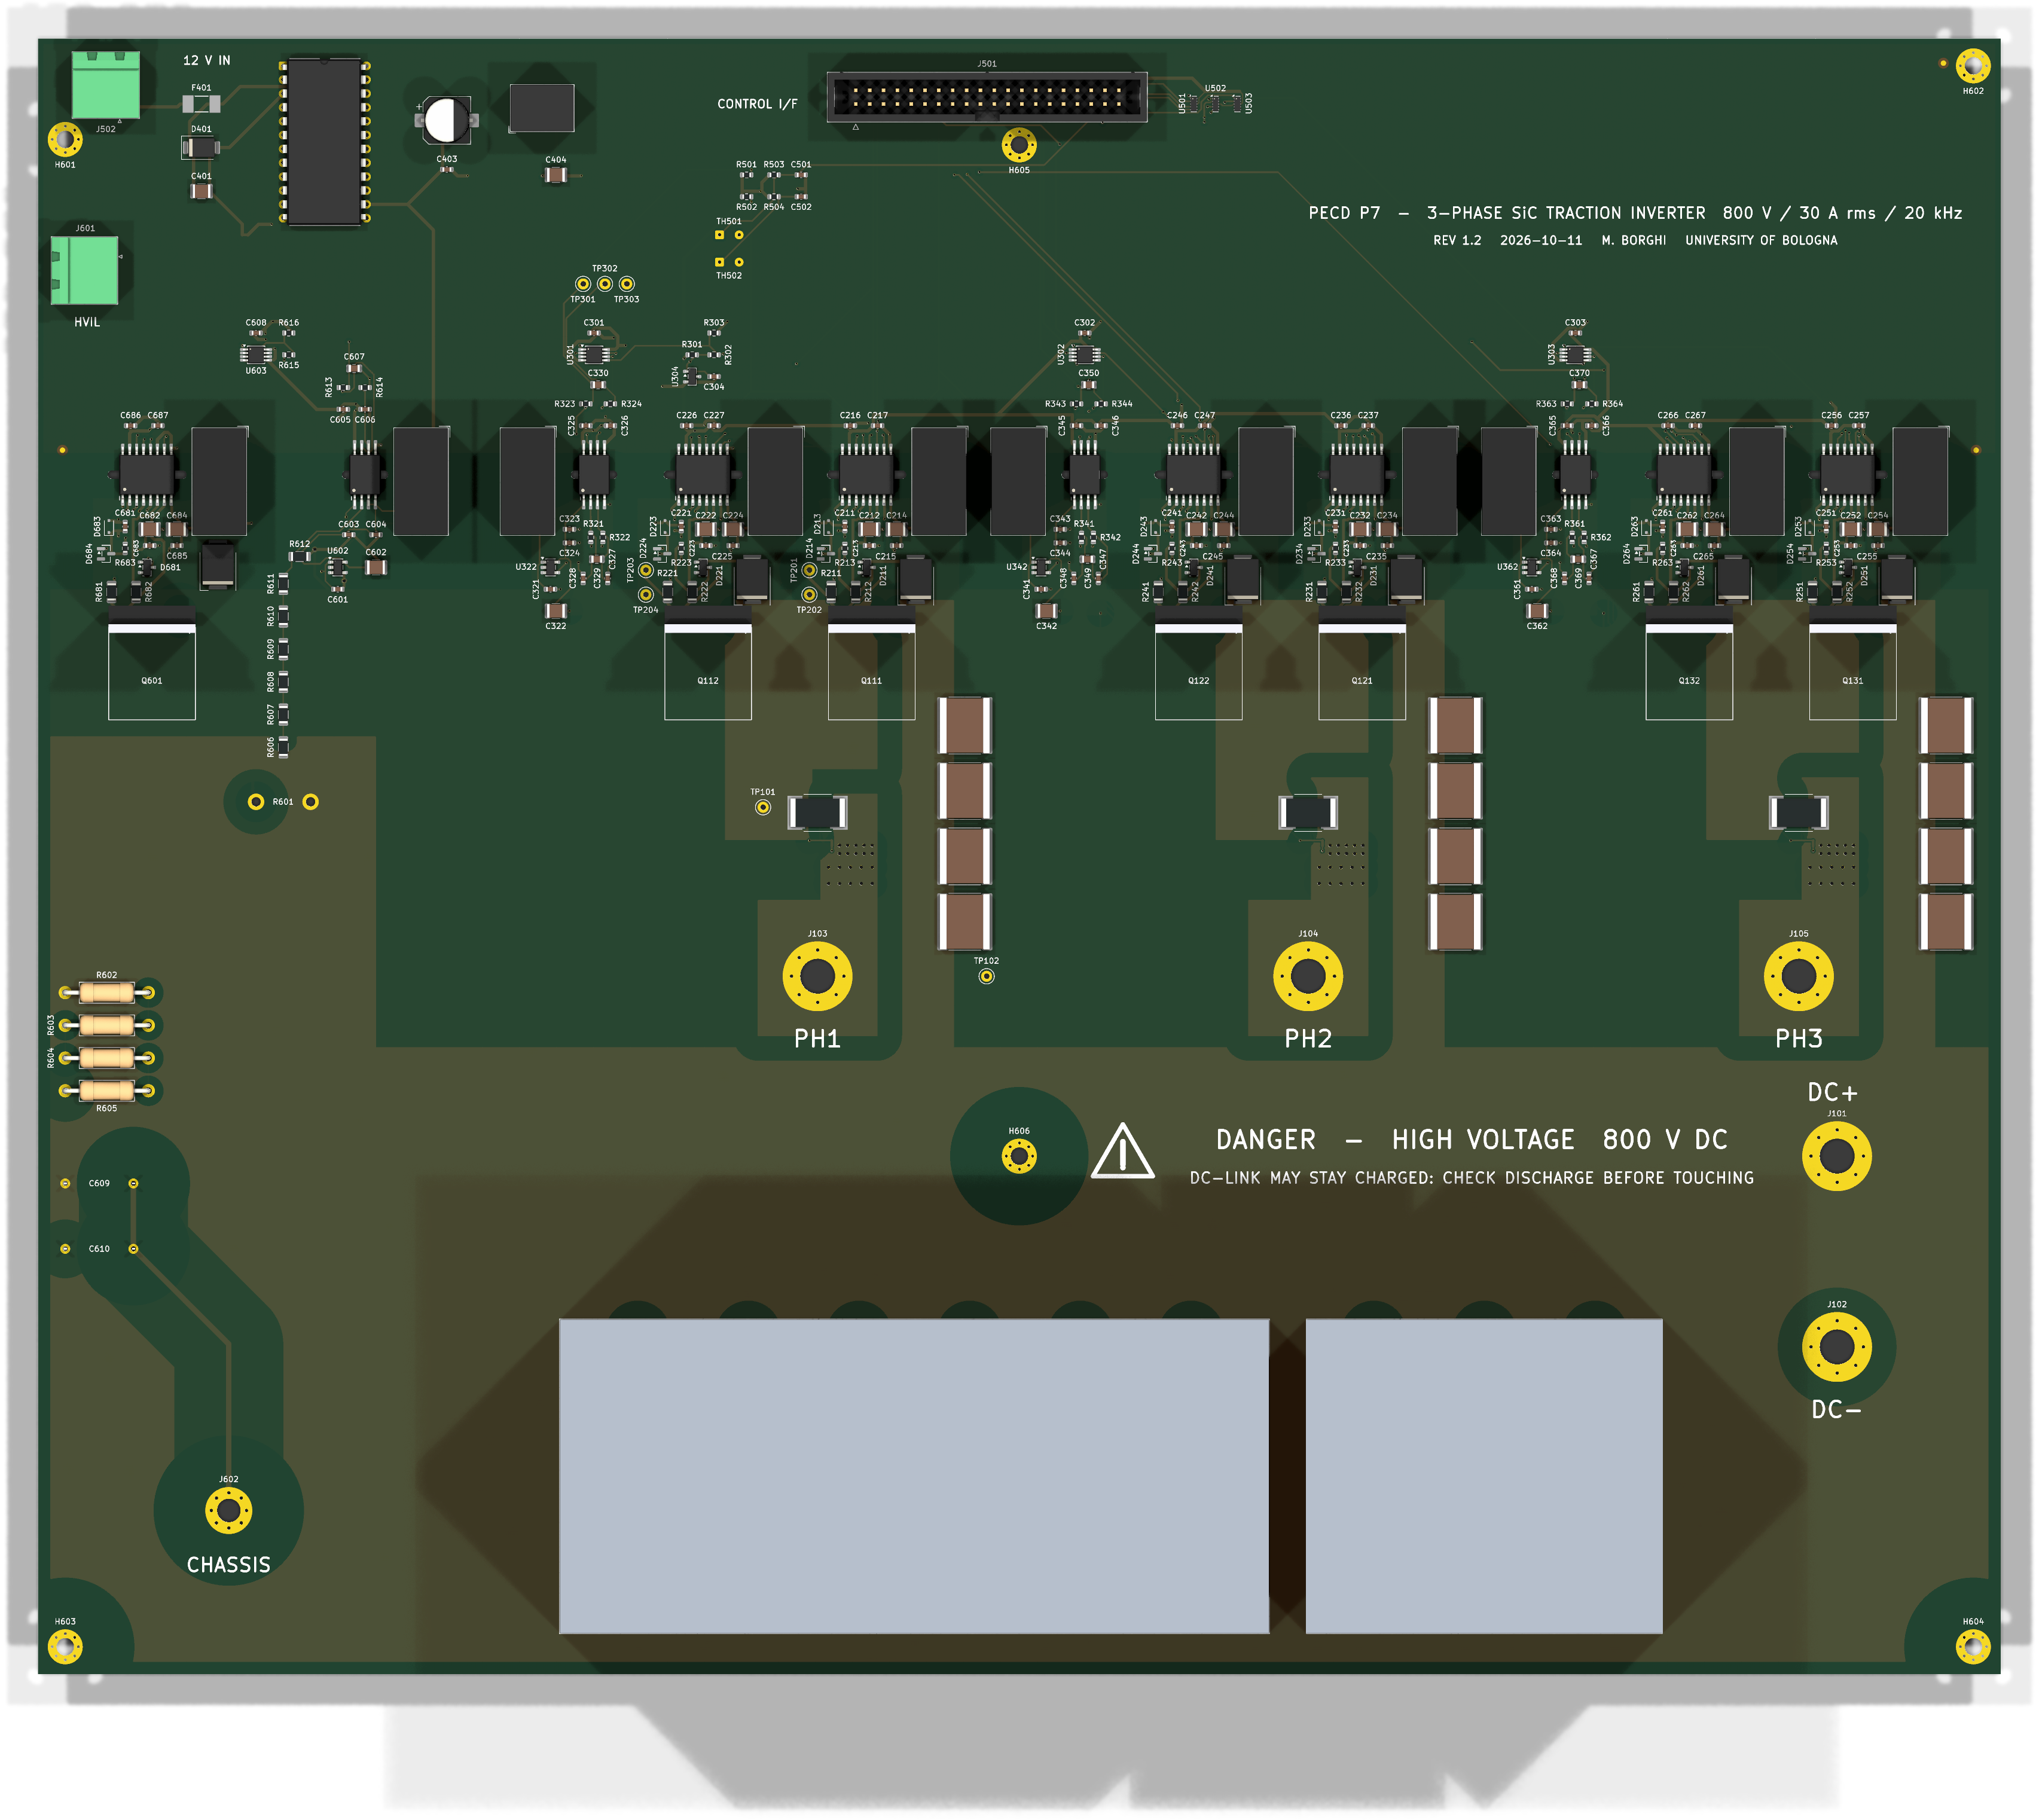
\includegraphics[width=\textwidth]{figures/kicad_3d_alto.png}
  \caption{The board seen from above, \SI{360}{}$\times$\SI{300}{\milli\metre}
  (3D render of the frozen design; bodies of the custom parts are blocks with
  datasheet dimensions). Top to bottom: control connector, auxiliary supply and
  comparators; the row of isolators and isolated supplies astride the barrier;
  the seven TO-247-4L devices and their drivers; phase terminals and
  commutation ceramics; the film DC-link capacitors.}
  \label{fig:pcb-top}
\end{figure}

\begin{figure}[htbp]
  \centering
  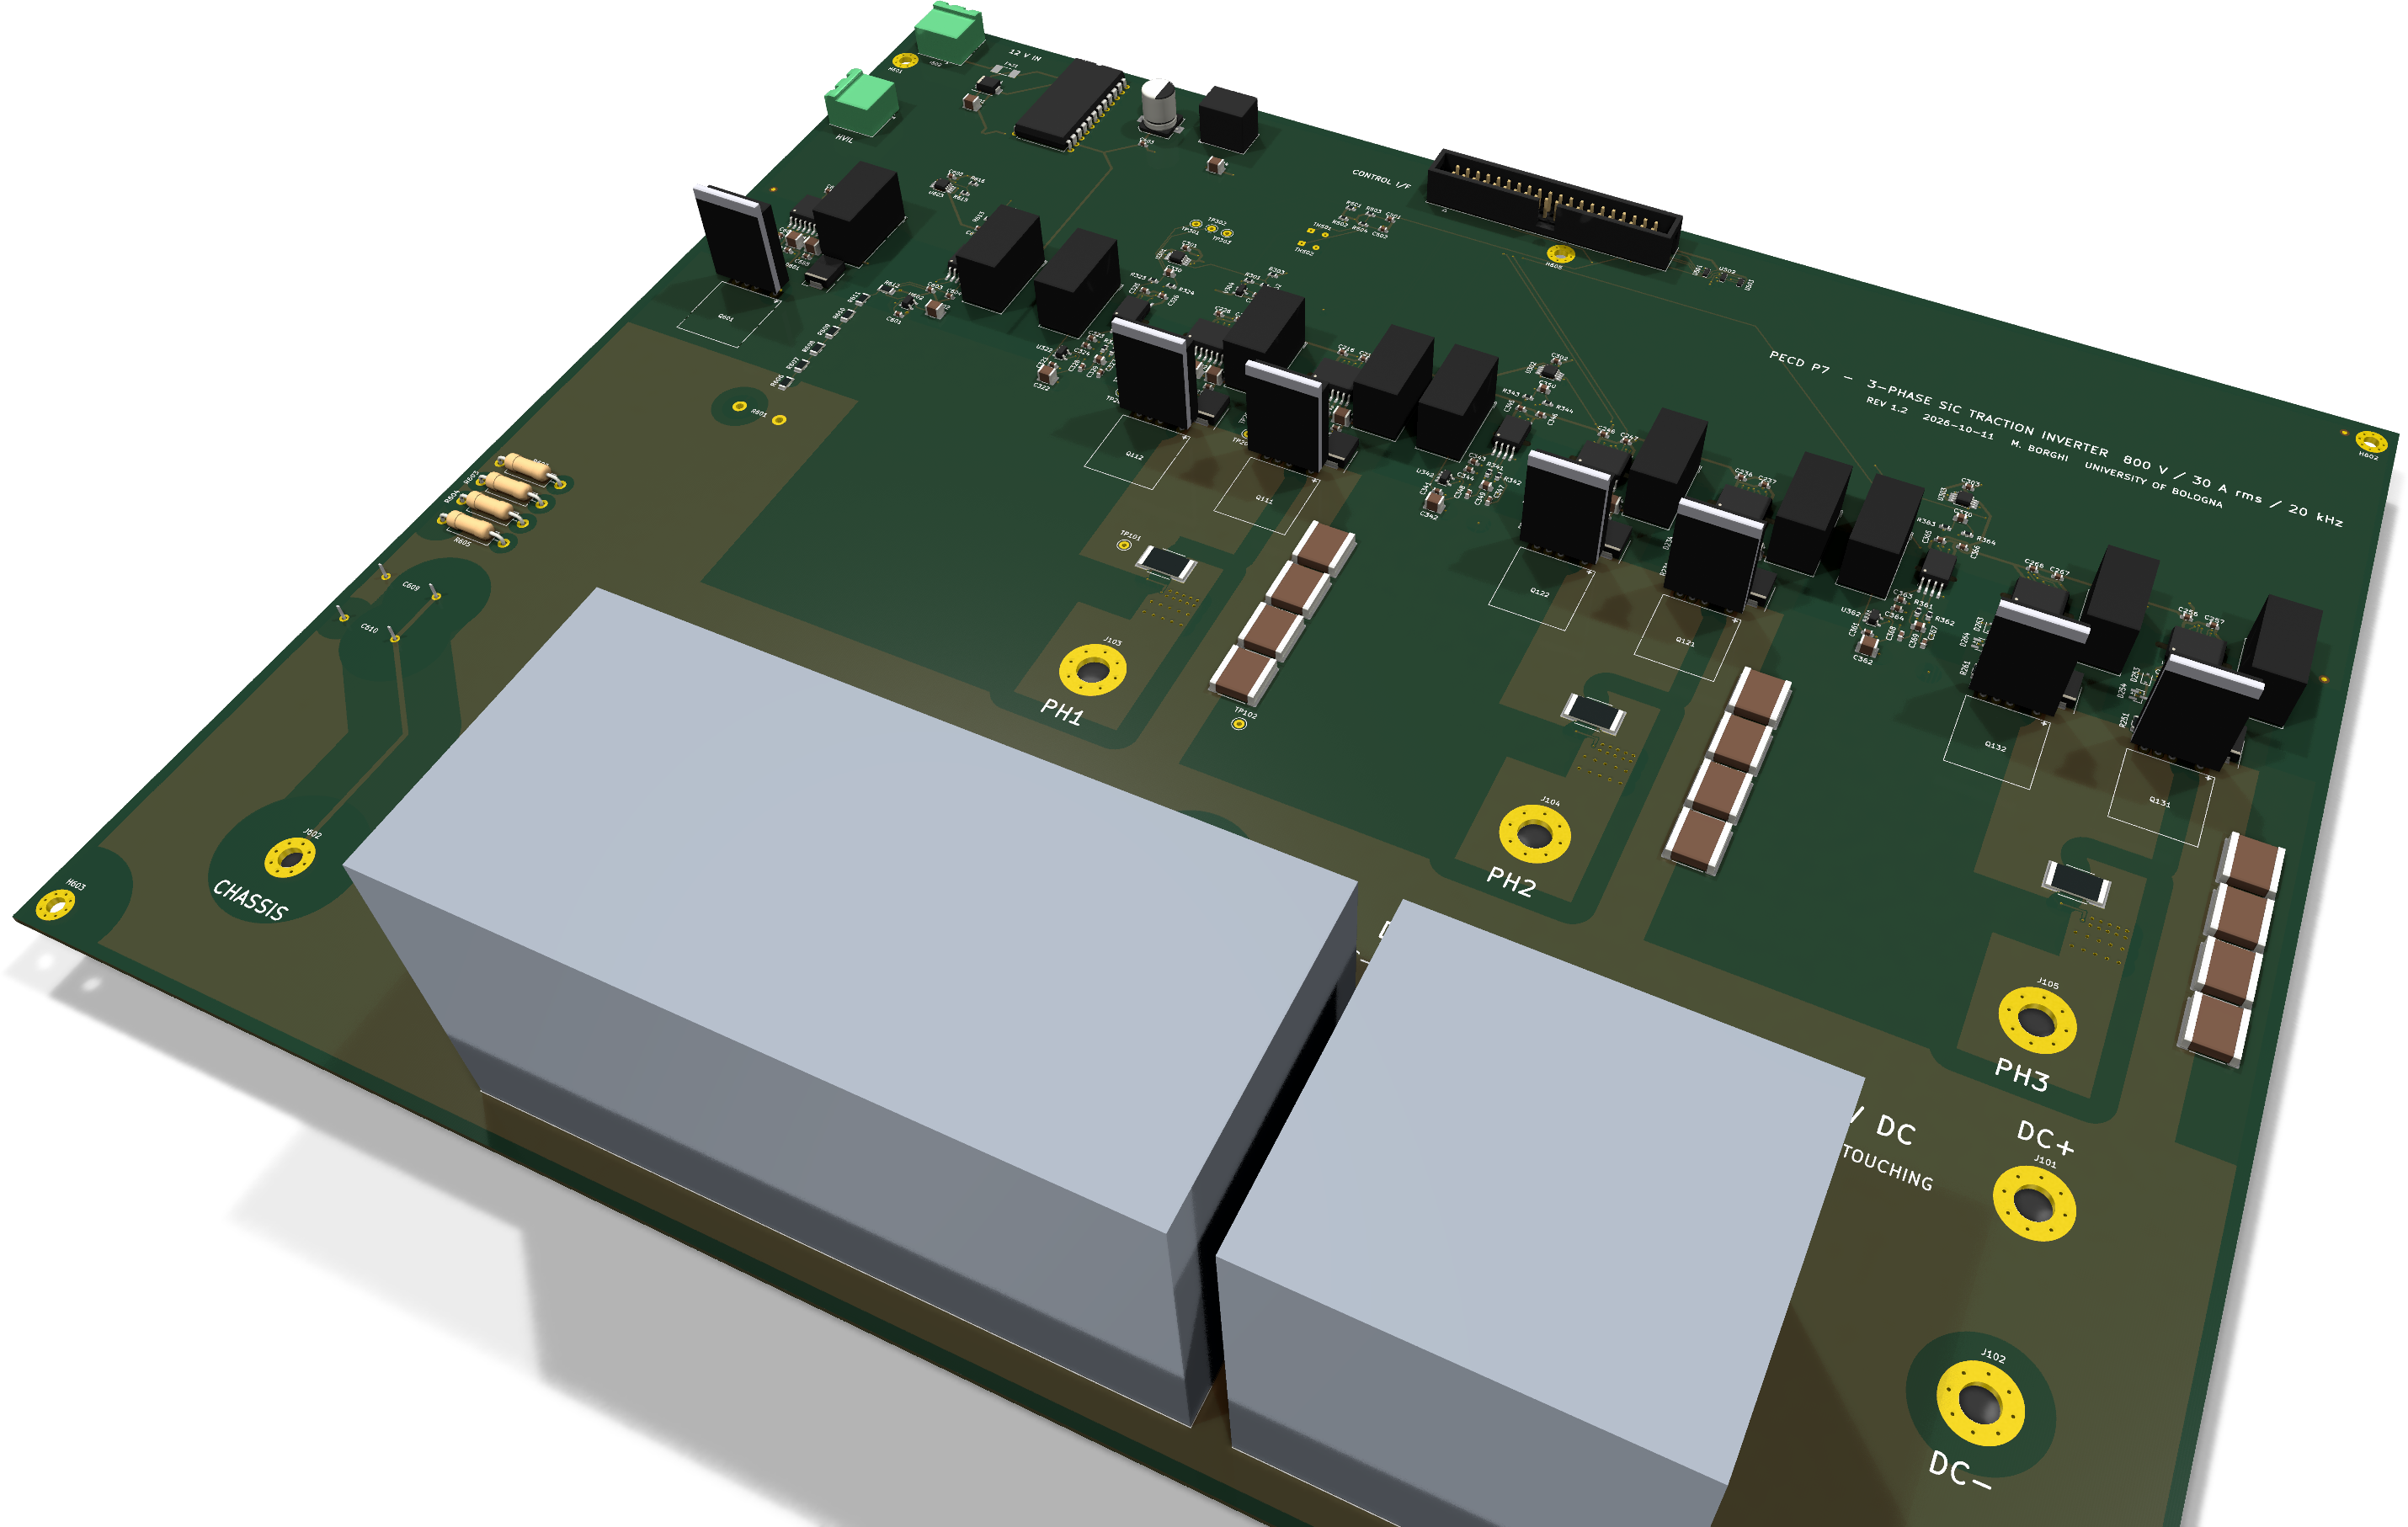
\includegraphics[width=\textwidth]{figures/kicad_3d_iso.png}
  \caption{3D view of the frozen board. The two film capacitors, \SI{65}{\milli\metre}
  tall, occupy the bottom fifth; the TO-247-4L stand vertically, tab towards
  the cold plate.}
  \label{fig:pcb-3d}
\end{figure}

\paragraph{Floorplan.} Everything is on one board
(\cref{fig:pcb-top,fig:pcb-3d}), for three reasons that have numbers behind
them. A connector between a driver board and a power board would add a
pair of parallel pins to every gate loop, about \SI{8}{\nano\henry} for
\SI{10}{\milli\metre} of stacking height; the common-mode current that the
barriers carry, \SI{0.80}{\ampere} peak (\cref{tab:cmcap}), returns on the
board's own ground plane instead of through a cable; and the reinforced
barrier is a single straight line, \SI{80}{\milli\metre} from the top edge,
that every isolator straddles and the design rules check in one piece.
The cost of one board (area that is six-layer even where two layers would
do, and a board lost to any power fault) is accepted for a prototype.

The floorplan follows the domains from top to bottom. The low-voltage side,
above the barrier, carries the control connector, the auxiliary supply, the
overload comparators and the thermistor inputs. On the barrier sit the eleven
isolators (seven \driver{}, three \isoamp{}, one \isoampv{}), each beside its
isolated supply. Below it, each driver faces its own device across a few
millimetres, so the gate loop never leaves its channel. The phase terminals
and the commutation ceramics follow, and the film capacitors fill the bottom
of the board. Six M3 fixing holes, without a net and \SI{9.5}{\milli\metre}
from all high-voltage copper, hold a board of this size against flexing,
which would otherwise fatigue the joints of the film capacitors.

\begin{table}[htbp]
\centering
\caption{The frozen board in numbers.}
\label{tab:boardnumbers}
\small
\begin{tabularx}{\textwidth}{lY}
\toprule
Outline & \SI{360}{}$\times$\SI{300}{\milli\metre}, six layers, \SI{1.6}{\milli\metre} \\
Parts & 275, all on the top side; 271 visible references (the four net ties carry none) \\
Nets & 143, plus 52 single-pin nets of unused pins \\
Tracks & 2168 segments, \SI{8.5}{\metre} in all, every one at \SI{0}{}, \SI{45}{} or \SI{90}{\degree} \\
Vias & 467: 50 on the negative DC rail, 60 stitching the phase pours to L6 \\
Copper pours & positive DC rail on L1 (\SI{411}{\centi\metre\squared}); negative DC plane on L2
  (\SI{627}{\centi\metre\squared}); ground on L3 and L5 (\SI{259}{\centi\metre\squared} each);
  switching nodes and phases on L1; ten floating-reference islands and the three
  phase pours of revision 1.1 on L6 \\
\bottomrule
\end{tabularx}
\end{table}

\paragraph{How the layers are used.} \Cref{fig:layers} shows the six copper
layers. The negative DC plane on L2 lies under the power stage only, and the
two ground planes on L3 and L5 under the low-voltage area only: the two never
overlap in plan, so no high-voltage plane faces a ground plane across a thin
dielectric. L4 carries the signals that cannot stay on the surface, the
sensing pairs among them. L6 carries one copper island per floating domain,
the seven gate references and the four sensing references, each under its
own driver or amplifier; an island is the return path of the gate loop above
it. Since revision 1.1 it also carries a second phase pour under each shunt
(\cref{sec:conductors}).

\begin{figure}[htbp]
  \centering
  \begin{subfigure}{0.49\textwidth}\centering
    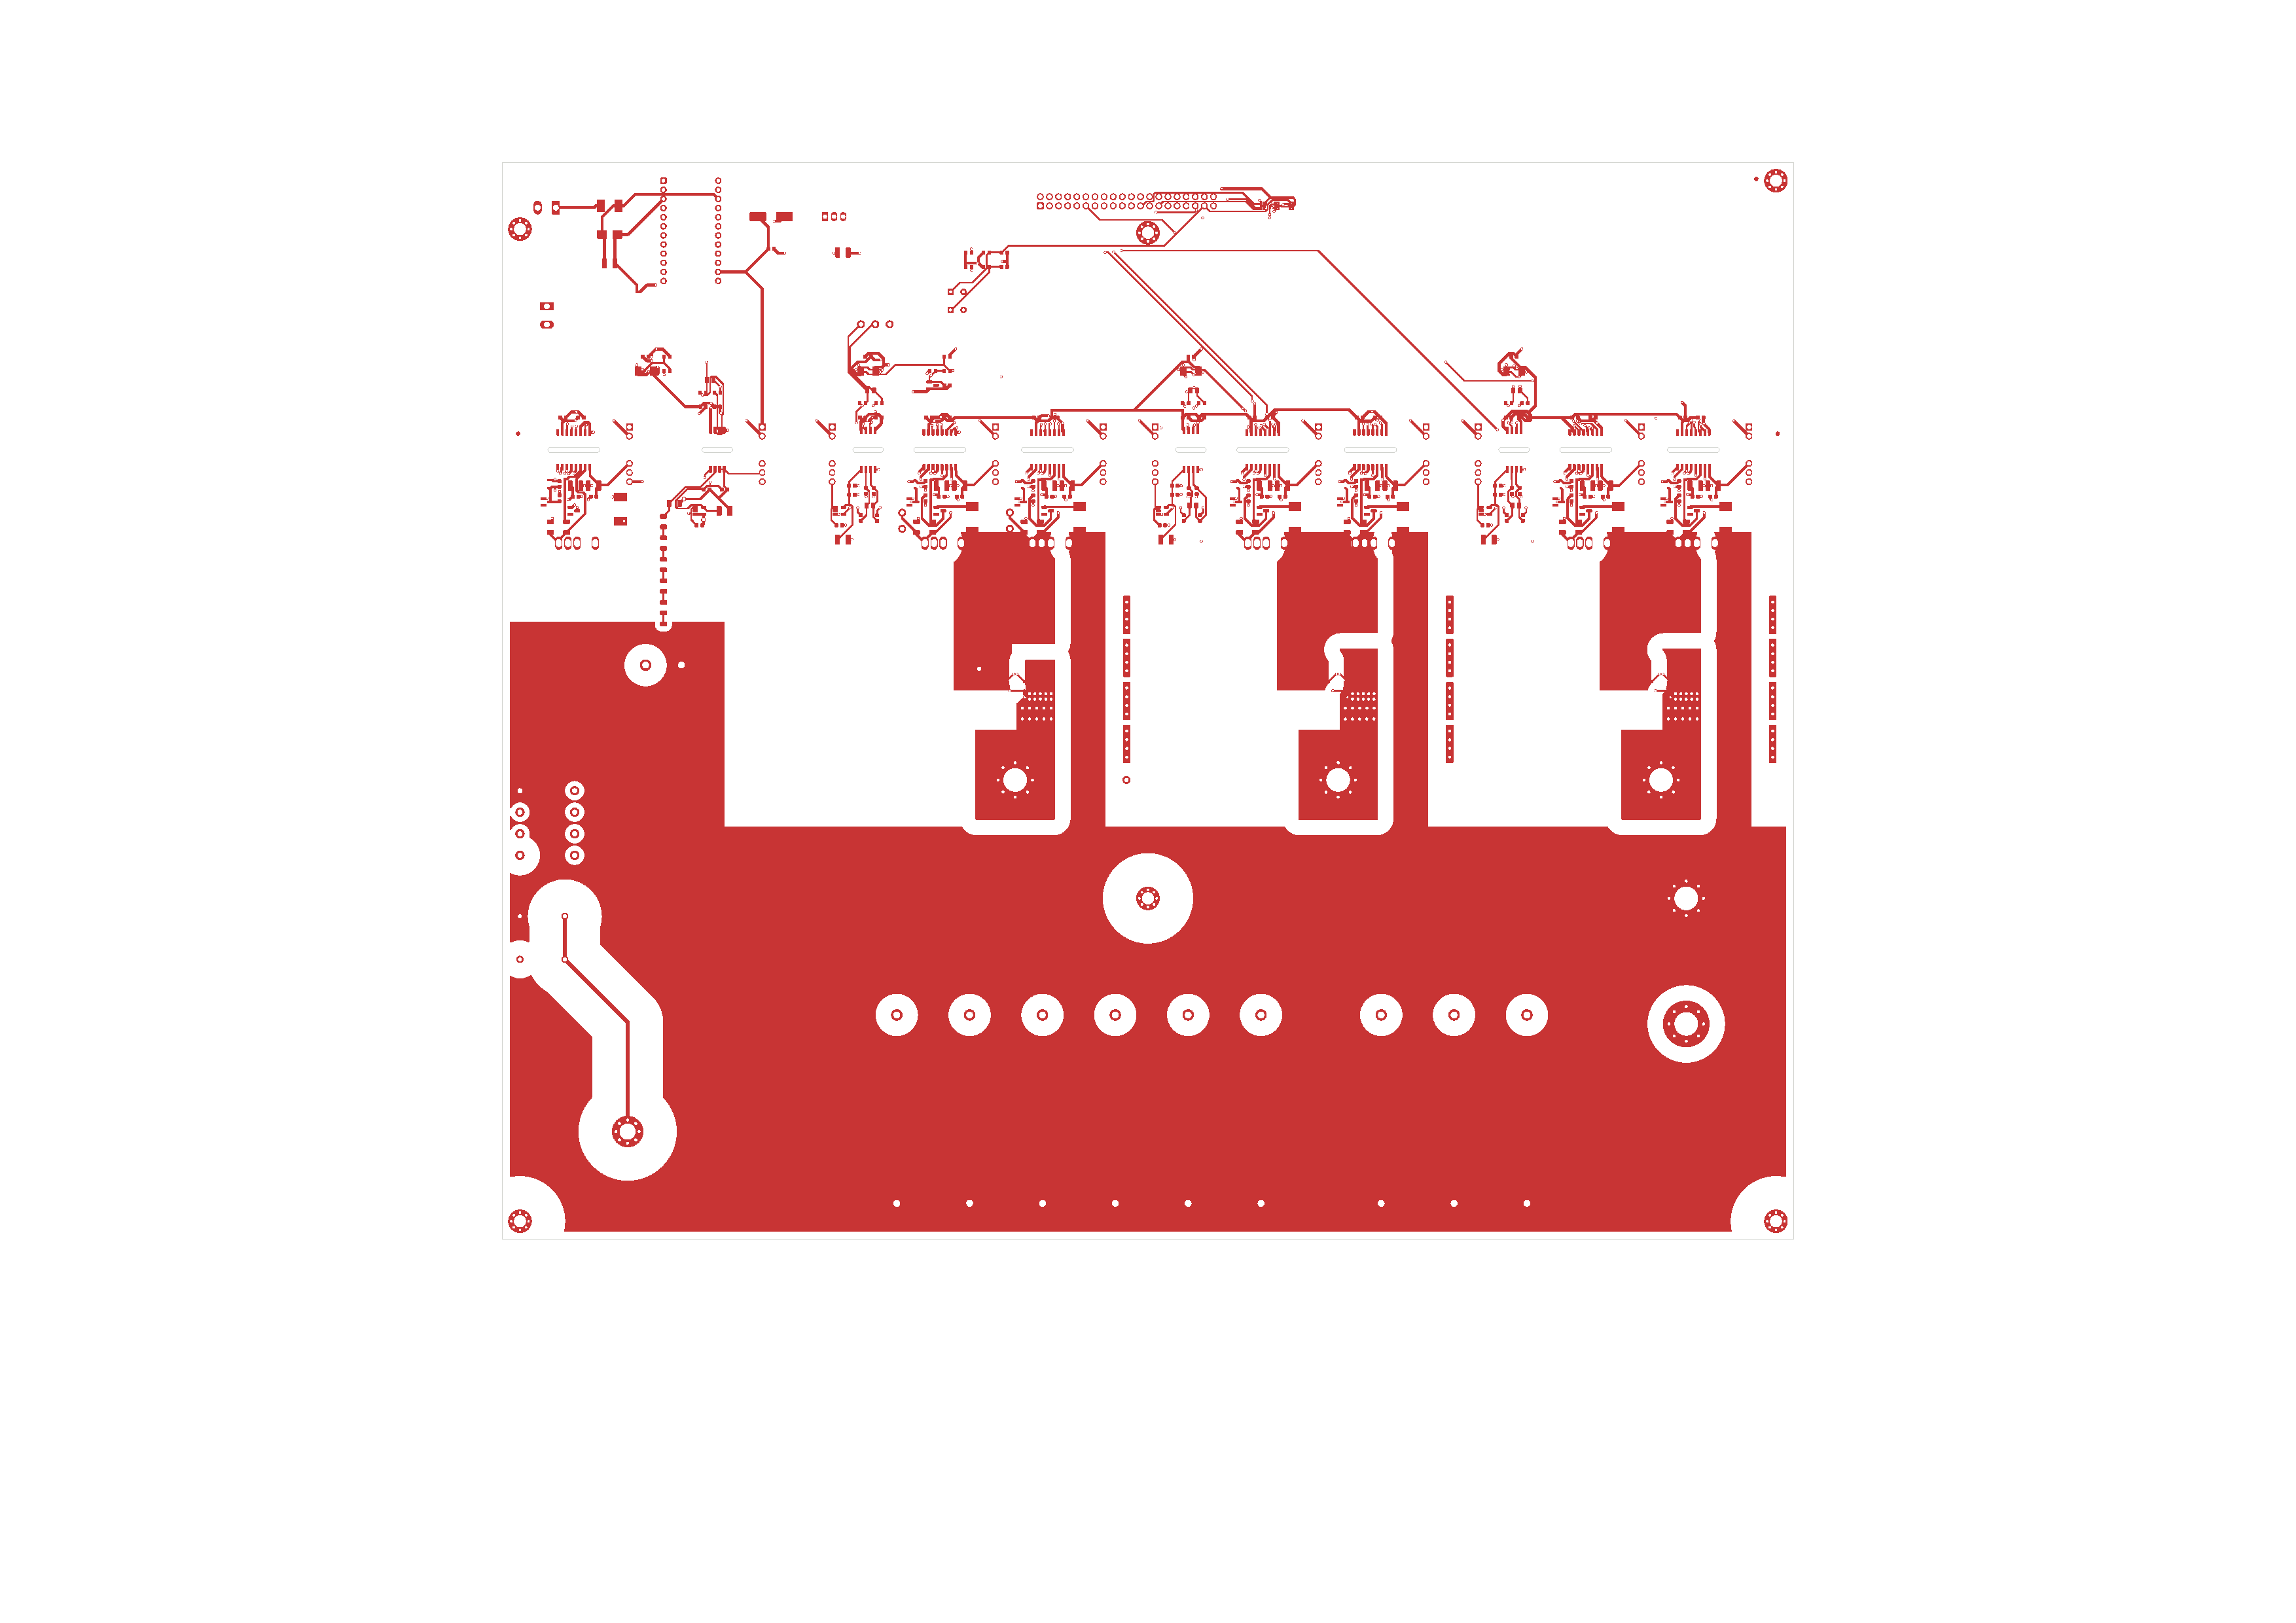
\includegraphics[page=1,width=\textwidth,trim=60mm 40mm 60mm 40mm,clip]{figures/kicad_strati.pdf}
    \caption{L1, top: power pours, components}\end{subfigure}\hfill
  \begin{subfigure}{0.49\textwidth}\centering
    \includegraphics[page=2,width=\textwidth,trim=60mm 40mm 60mm 40mm,clip]{figures/kicad_strati.pdf}
    \caption{L2: negative DC plane, control signals}\end{subfigure}\\[2mm]
  \begin{subfigure}{0.49\textwidth}\centering
    \includegraphics[page=3,width=\textwidth,trim=60mm 40mm 60mm 40mm,clip]{figures/kicad_strati.pdf}
    \caption{L3: ground plane}\end{subfigure}\hfill
  \begin{subfigure}{0.49\textwidth}\centering
    \includegraphics[page=4,width=\textwidth,trim=60mm 40mm 60mm 40mm,clip]{figures/kicad_strati.pdf}
    \caption{L4: signals, sensing pairs}\end{subfigure}\\[2mm]
  \begin{subfigure}{0.49\textwidth}\centering
    \includegraphics[page=5,width=\textwidth,trim=60mm 40mm 60mm 40mm,clip]{figures/kicad_strati.pdf}
    \caption{L5: ground plane}\end{subfigure}\hfill
  \begin{subfigure}{0.49\textwidth}\centering
    \includegraphics[page=6,width=\textwidth,trim=60mm 40mm 60mm 40mm,clip]{figures/kicad_strati.pdf}
    \caption{L6, bottom: floating-reference islands, phase pours}\end{subfigure}
  \caption{The six copper layers of the frozen board.}
  \label{fig:layers}
\end{figure}

\paragraph{Routing.} Every channel was routed once and copied to its twins by
translation, so the seven gate loops are the same copper and the three
sensing channels the same pairs; the local low-voltage nets were routed
partly by an autorouter fed with the class clearances and partly by hand.
Tracks run only at \SI{0}{}, \SI{45}{} and \SI{90}{\degree}.

\begin{figure}[htbp]
  \centering
  \begin{subfigure}{0.48\textwidth}\centering
    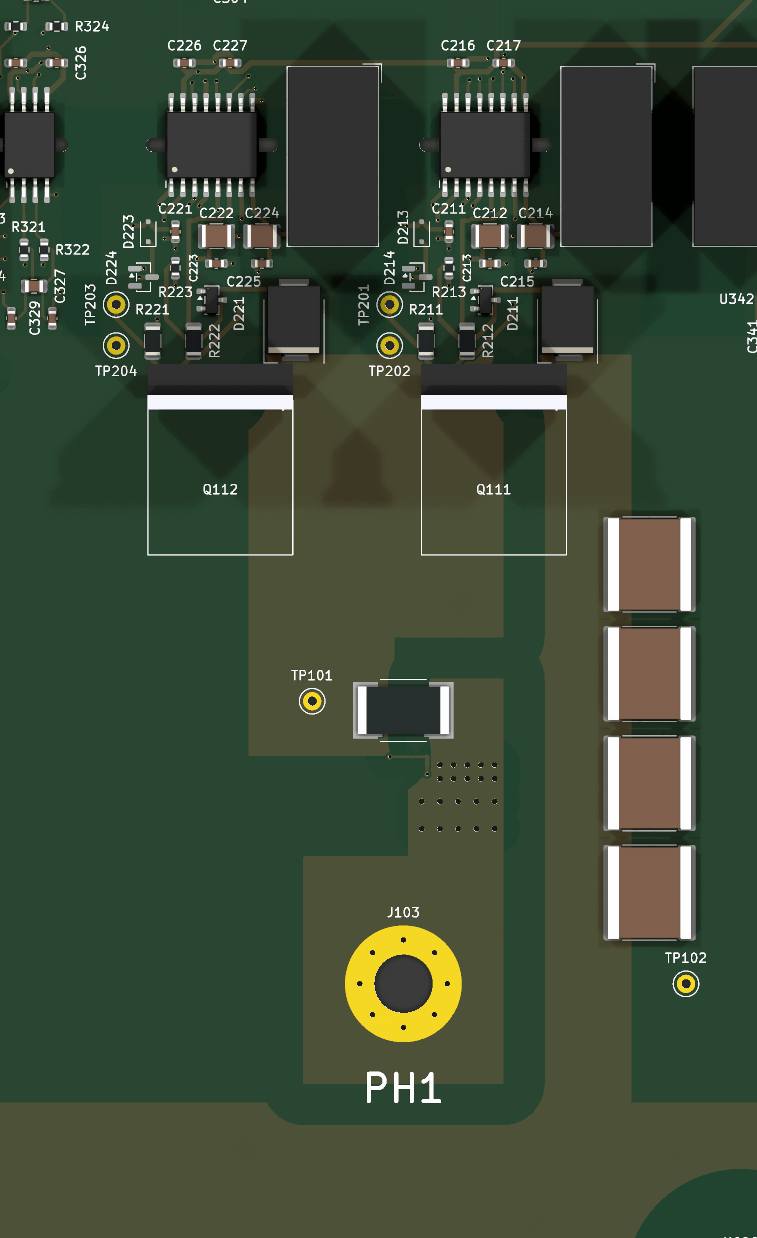
\includegraphics[height=10.5cm,keepaspectratio]{figures/kicad_3d_ramo.png}
    \caption{3D, top}\end{subfigure}\hfill
  \begin{subfigure}{0.48\textwidth}\centering
    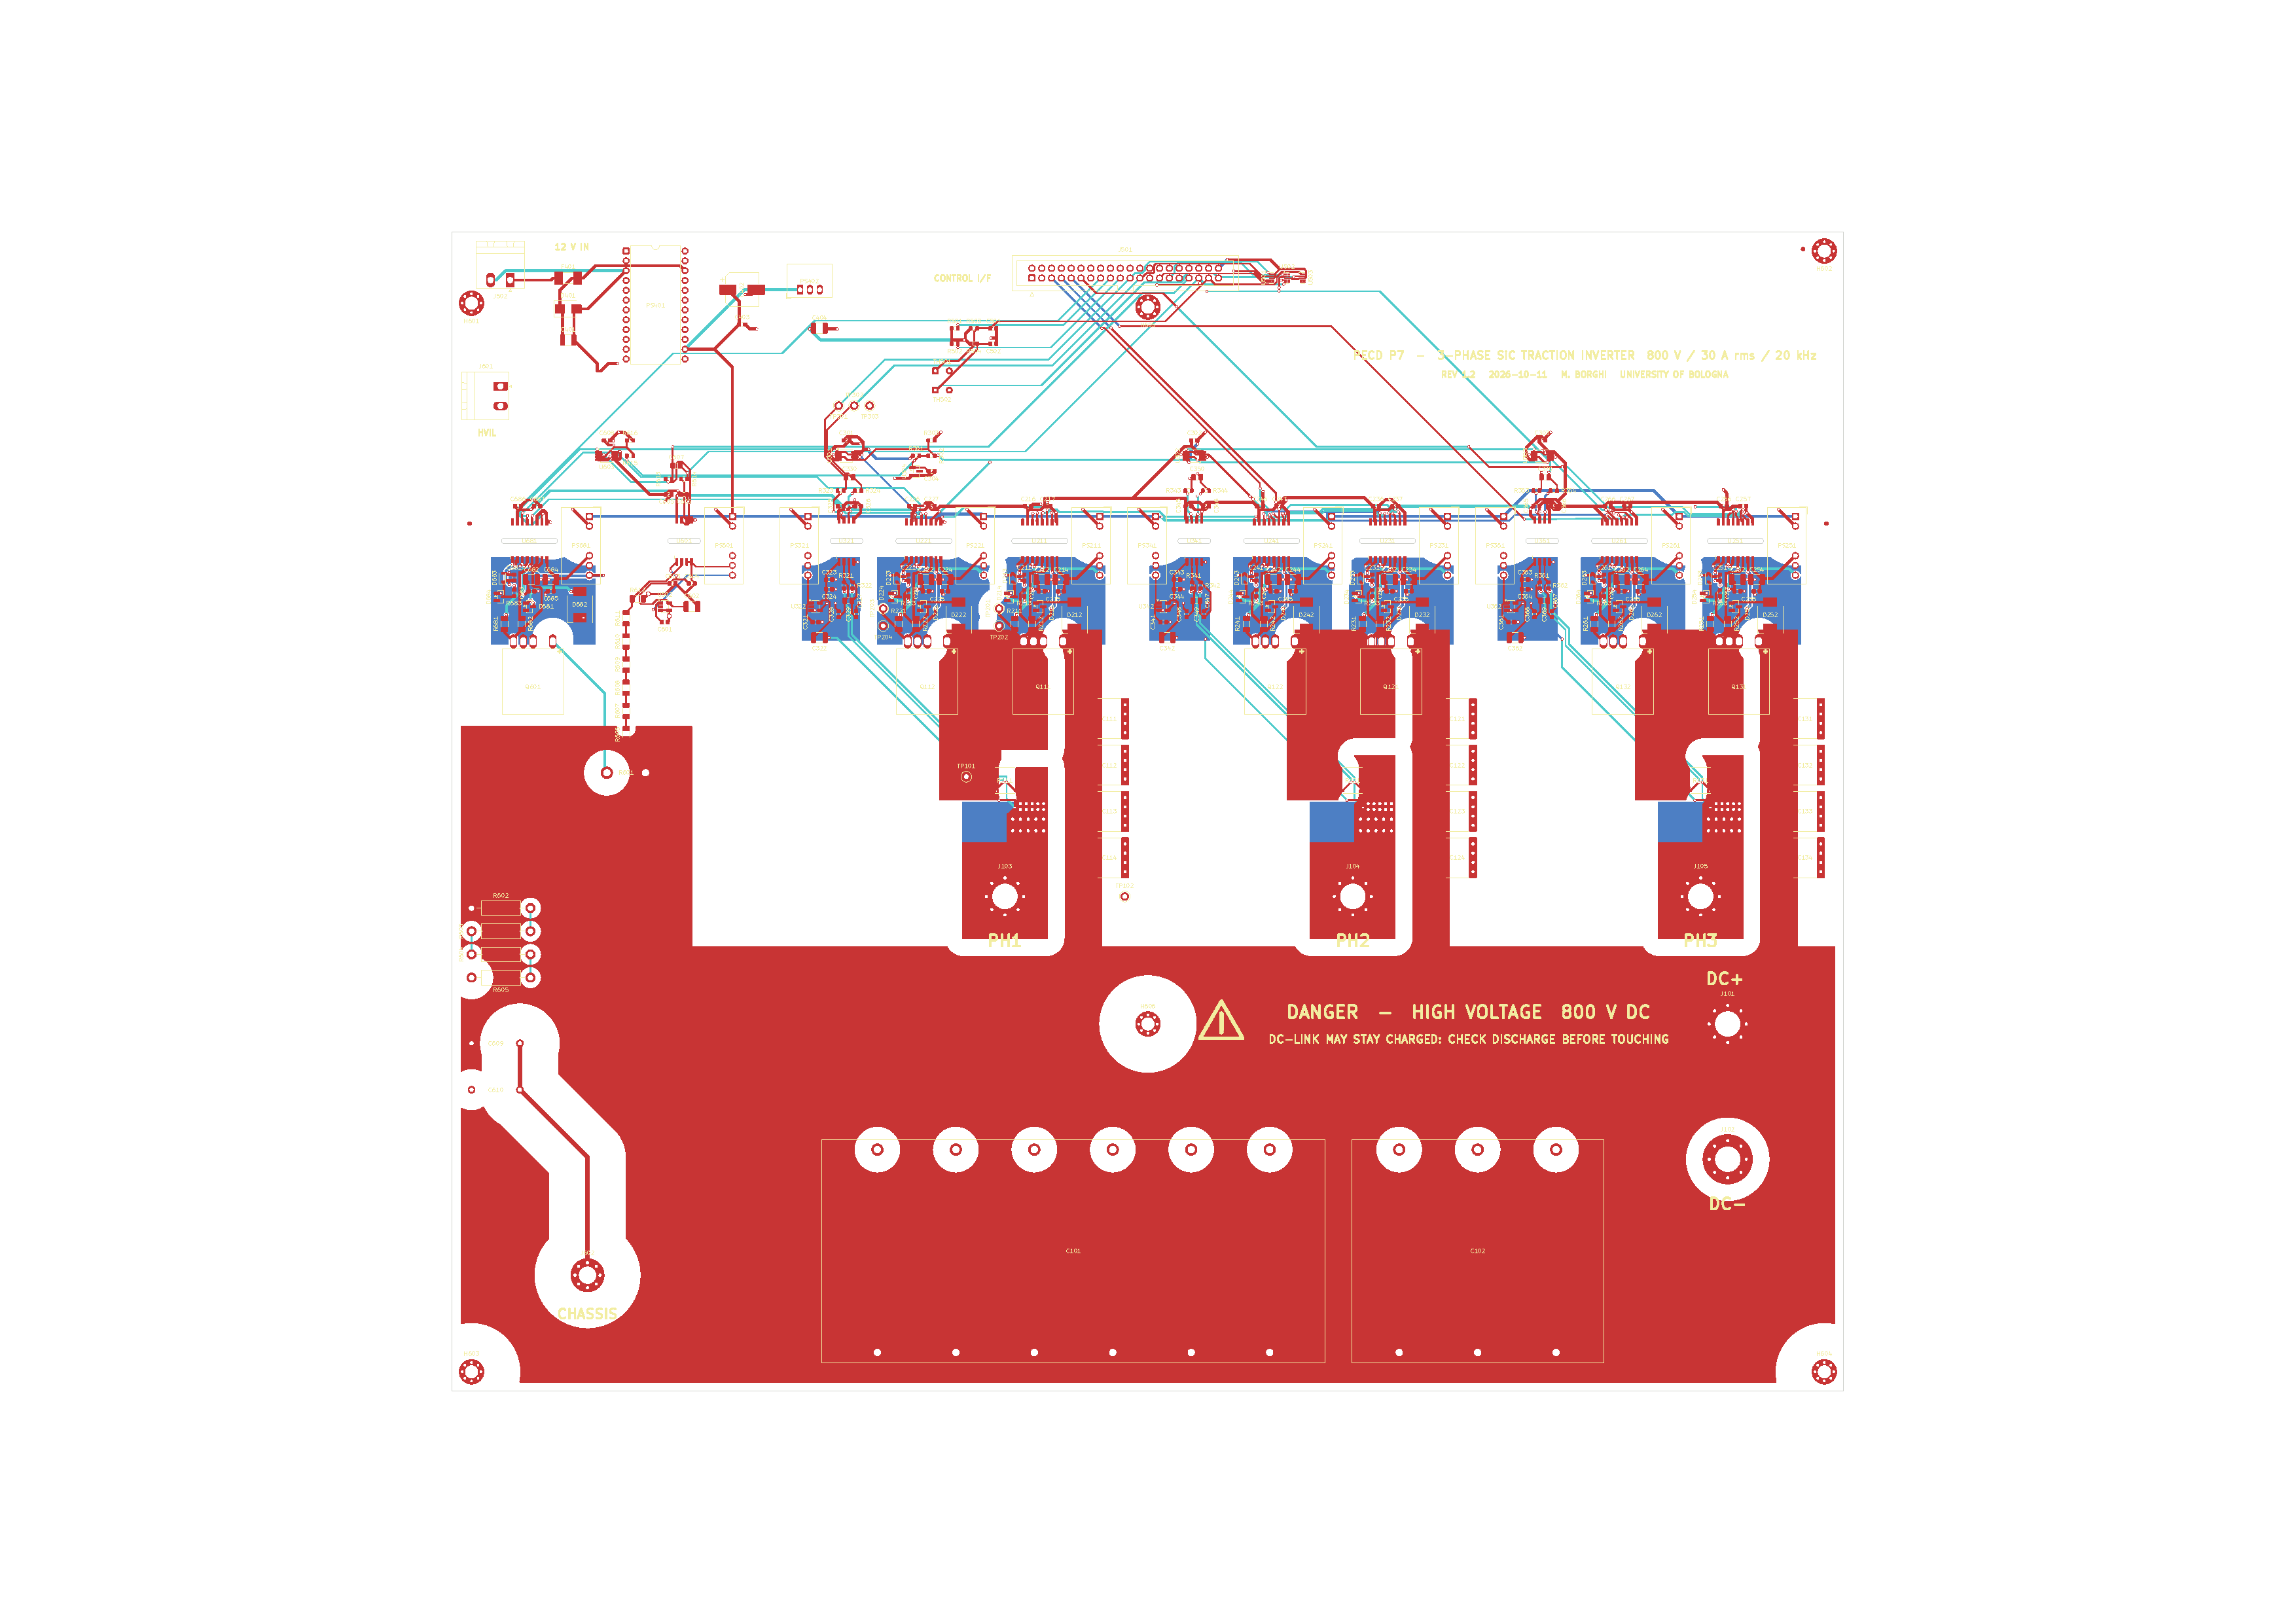
\includegraphics[height=10.5cm,trim=219mm 174mm 295mm 124mm,clip]{figures/kicad_rame_canale.pdf}
    \caption{copper: L1 (red), L4 (cyan), L6 (blue)}\end{subfigure}
  \caption{Leg 1 with its two driver channels: drivers on the barrier, gate
  resistors and desaturation diode between driver and device, the shunt in
  the source path, the four commutation ceramics on the right, the phase
  terminal at the bottom.}
  \label{fig:pcb-leg}
\end{figure}

\paragraph{The gate loop, measured on the copper.} The target of
\SI{25}{\milli\metre} from driver output to gate was set before routing.
Along the tracks of the frozen board it is \SI{23.7}{\milli\metre}
at turn-on and \SI{24.3}{\milli\metre} at turn-off, the same in all seven
channels (\cref{fig:pcb-leg}). The turn-on path dips to L4 through two vias
to clear the parts around the driver; there it runs \SI{0.6}{\milli\metre}
above the reference island on L6 that carries the return, which is closer
than a surface track could get, so the loop is narrower as well as shorter.
Extracted from the copper with the method of \cref{sec:loopextract}, the
loop from the driver output through the gate resistor to the gate, and back
from the Kelvin pin through the island to the driver reference, is
\SI{13}{\nano\henry} (grids of 0.40, 0.30 and
\SI{0.25}{\milli\metre}: 14.3, 13.4, \SI{13.3}{\nano\henry}). That is
consistent with a \SI{0.5}{\milli\metre} track \SI{0.6}{\milli\metre}
above its return, about \SI{0.5}{\nano\henry\per\milli\metre}, and it is
more than the \SI{5}{\nano\henry} the switching simulation had assumed. Its
effect is small (\cref{tab:dptextract}): the gate resistance is above the
critical value $2\sqrt{L/C_\mathrm{iss}}$, so the loop does not ring, and
the peaks move by a few volts.

\paragraph{The sensing pairs.} The two Kelvin connections from each shunt to
its amplifier run side by side on L4, \SI{0.9}{\milli\metre} apart over
\SI{90}{\percent} of their length, \SI{70}{} to \SI{80}{\milli\metre} long.
The two halves of a pair differ in length by up to \SI{8}{\milli\metre}; at
the bandwidth of the measurement that is irrelevant. What matters is the
area enclosed between the two conductors, which picks up the field of the
phase current, and keeping them together keeps it small.

\section{Stack-up}
\label{sec:stackup}

\begin{table}[htbp]
\centering
\caption{Six-layer stack-up, as in the board file. Finished thickness
\SI{1.6}{\milli\metre}.}
\label{tab:stackup}
\begin{tabular}{llll}
\toprule
Layer & Copper & Function & Dielectric below \\
\midrule
L1 & \SI{2}{oz} & power: DC-positive, switching nodes, terminals & prepreg \SI{0.10}{\milli\metre} \\
L2 & \SI{1}{oz} & \textbf{DC-negative plane} (power area); control signals & core \SI{0.46}{\milli\metre} \\
L3 & \SI{1}{oz} & ground plane (low-voltage area) & prepreg \SI{0.20}{\milli\metre} \\
L4 & \SI{1}{oz} & signals: gate turn-on path, sensing pairs, control & core \SI{0.46}{\milli\metre} \\
L5 & \SI{1}{oz} & ground plane (low-voltage area) & prepreg \SI{0.10}{\milli\metre} \\
L6 & \SI{2}{oz} & floating-reference islands of drivers and amplifiers & --- \\
\bottomrule
\end{tabular}
\end{table}

The cores are \SI{0.46}{\milli\metre} rather than the \SI{0.40}{} first
considered, so that the stack adds up to the standard
\SI{1.6}{\milli\metre}; only the L1--L2 prepreg matters electrically, and it
is unchanged.

\paragraph{Six layers or four.} Before routing, a four-layer board looked
equivalent: the negative DC plane and the ground planes never overlap in
plan, so they could have shared one layer, with one signal layer below it.
The routed board uses both inner signal layers: L4 carries
\SI{3.4}{\metre} of track (the turn-on half of every gate loop and all the
sensing pairs among it), and L2 another \SI{1.2}{\metre} of control signals
above the barrier. A four-layer version would have to fit both into one
layer and keep a single ground plane under the control area. That was not
attempted, so the six layers are justified by the density the routing
reached, not proven necessary; at a production cost review it is the first
thing to try.

The one dimension that the stack-up exists to fix is the L1--L2 prepreg. Two
facing planes carrying a current and its return have
%
\begin{equation}
  L = \frac{\mu_0\,h\,l}{w},
  \label{eq:planepair}
\end{equation}
%
proportional to the separation $h$. For the \SI{30}{\milli\metre} by
\SI{20}{\milli\metre} region that the commutation loop occupies:

\begin{table}[htbp]
\centering
\caption{Plane-pair inductance against prepreg thickness,
$l = \SI{30}{\milli\metre}$, $w = \SI{20}{\milli\metre}$.}
\label{tab:planepair}
\begin{tabular}{lr}
\toprule
L1--L2 separation & Inductance \\
\midrule
\SI{0.075}{\milli\metre} & \SI{0.141}{\nano\henry} \\
\SI{0.10}{\milli\metre} (selected) & \SI{0.188}{\nano\henry} \\
\SI{0.20}{\milli\metre} & \SI{0.377}{\nano\henry} \\
\SI{0.36}{\milli\metre} (standard core) & \SI{0.679}{\nano\henry} \\
\bottomrule
\end{tabular}
\end{table}

\begin{finding}{The plane pair is not where the inductance budget is spent}
Against a target of \SI{20}{\nano\henry} the plane pair contributes under
\SI{0.7}{\nano\henry} even with a standard \SI{0.36}{\milli\metre} core. The
thin prepreg is still specified, because it costs nothing and every tenth of
a nanohenry saved stays available elsewhere, but it is not the decisive
choice. The budget is spent on vertical transitions (vias, pads, the leads
between board and device) and on the path to the ceramic capacitors.

A corollary follows: if \SI{0.10}{\milli\metre} ever
becomes awkward, doubling it costs \SI{0.19}{\nano\henry} and halves the
electric stress in the solid insulation from \SI{9}{} to
\SI{4.5}{\kilo\volt\per\milli\metre} at \SI{900}{\volt}
(\cref{sec:insulation}). That is a good
trade, and it should be reconsidered at the first prototype.
\end{finding}

\begin{table}[htbp]
\centering
\caption{Commutation loop budget, estimated before layout; the last rows
give the extraction from the frozen board (\cref{sec:loopextract}).}
\label{tab:loopbudget}
\small
\begin{tabular}{lrl}
\toprule
Contribution & [\si{\nano\henry}] & Controlled by layout? \\
\midrule
Device packages & 14.6 & no \\
Leads and pads & 3--6 & partly: short leads \\
Vias and vertical transitions & 0.4--2 & yes \\
Plane pair L1--L2 & 0.19 & yes, and already negligible \\
Ceramic capacitor ESL & 1--2 & yes: more parts in parallel \\
\midrule
\textbf{Board-attributable total} & \textbf{5--10} & target \SI{20}{\nano\henry}: reachable \\
\textbf{Physical loop} & \textbf{20--25} & \\
\midrule
Extracted, revision 1.0: board copper & 12$\pm$1 & three legs alike \\
\quad of which at the clearance holes & 7.7 & yes: inner-layer clearance \\
\textbf{Extracted, revision 1.1: board copper} & \textbf{7.8} & inner-layer clearance relaxed \\
\textbf{Revision 1.1, with capacitor ESL} & \textbf{about 8.3} & \SI{14}{\nano\henry} to the C2 threshold \\
\bottomrule
\end{tabular}
\end{table}

\section{Commutation loop}

The limit is \SI{20}{\nano\henry} of PCB-attributable inductance and the
failure threshold \SI{22.6}{\nano\henry}. The limit is a design input: the gate resistances of \SI{5}{}/\SI{12.5}{\ohm} were
chosen so that the die stays below \SI{1080}{\volt} at \SI{950}{\volt} and
\SI{60}{\ampere} \emph{with} \SI{20}{\nano\henry} (\cref{sec:kelvin}). The
frozen board's loop is extracted below (\cref{sec:loopextract}) and still
to be measured (test B2 of \cref{tab:benchplan}); both are to be checked
against the threshold at which C2 is
lost, \SI{22.6}{\nano\henry} at turn-off and
\SI{23.6}{\nano\henry} on recovery (\cref{tab:lthreshold}), not only
against the limit: the \SI{2.6}{\nano\henry} between them is the whole
margin, and above \SI{23}{\nano\henry} the recovery peak rises four times
faster than the turn-off one. As established there, the device packages contribute a
further \SI{14.6}{\nano\henry} that no layout can remove, so the physical
loop will measure around \SI{35}{\nano\henry} at the limit and
\SIrange{20}{25}{\nano\henry} at the estimate of \cref{tab:loopbudget}.

\subsection{Extracted from the copper of the frozen board}
\label{sec:loopextract}

\paragraph{Method.} The loop of this board is made of pours, not tracks: the
positive rail and the switching node on L1, the negative plane on L2,
\SI{0.10}{\milli\metre} below. A track-based extraction does not see it,
so the copper of each leg was extracted with the partial-element method
that FastHenry uses. The filled copper of L1 and L2 is read from the board
file on a square grid; every pair of parallel cells has a mutual partial
inductance, computed in closed form along the cell and by integration
across it; the high-side device and each ceramic are ideal shorts between
their pads, and the loop is seen from the drain--source terminals of the
low-side device. Resistance is neglected, which is the high-frequency limit
that matters for the switching edge. The result is the \emph{board}
contribution, to which the packages (\SI{14.6}{\nano\henry}, in the
vendor's model) and the capacitor ESL are added.

The solver was checked before it was trusted: two parallel plates
\SI{10}{}$\times$\SI{30}{\milli\metre} at \SI{0.10}{\milli\metre} give
\SI{0.355}{\nano\henry} against \SI{0.364}{\nano\henry} from
\cref{eq:planepair}, the small deficit being the fringing the formula
ignores; a square loop of strip, a case with no plane at all, matches its
closed form within \SI{1}{\percent}. On the board, grids from
\SI{1.25}{} to \SI{0.8}{\milli\metre} give 11.7 to \SI{12.7}{\nano\henry}
without a trend, the scatter coming from how the pins fall on the grid.

\paragraph{Result.} Revision 1.0 gave \SI{12}{}$\pm$\SI{1}{\nano\henry} of
board copper, the same in the three legs, which are copies; the finding
below explains where it was spent and why revision 1.1 brings it to
\SI{7.8}{\nano\henry} (\SI{8.2}{\nano\henry} on the finer grid). The
ceramic datasheet gives no ESL; from the geometry of the body over the
plane, four in parallel add about \SI{0.5}{\nano\henry}. The
board-attributable loop of the frozen board is therefore about
\SI{8.3}{\nano\henry}: well below the \SI{20}{\nano\henry} on which the gate
resistances were chosen and \SI{14}{\nano\henry} from the
\SI{22.6}{\nano\henry} at which C2 is lost. The physical loop, packages
included, is about \SI{23}{\nano\henry}.

\paragraph{The switching simulation with the extracted values.} The
double-pulse bench of \cref{sec:kelvin} was run again with the extracted
loop and gate-loop inductances in place of the budget, and nothing else
changed; it reproduces the report's case exactly when given the budget.

\begin{table}[htbp]
\centering
\caption{Double pulse at \SI{950}{\volt}, \SI{60}{\ampere}, \SI{175}{\celsius},
$R_g$ \SI{5}{}/\SI{12.5}{\ohm}: the budget against the extracted board.
Peak at the die; limit \SI{1080}{\volt}.}
\label{tab:dptextract}
\small
\begin{tabular}{lrrrr}
\toprule
Case & Loop & Gate loop & Turn-off peak & Recovery peak \\
\midrule
Budget (\cref{sec:kelvin}) & \SI{20}{\nano\henry} & \SI{5}{\nano\henry} & \SI{1073.5}{\volt} & \SI{1050.0}{\volt} \\
Revision 1.0, extracted & \SI{12.5}{\nano\henry} & \SI{13}{\nano\henry} & \SI{1052.5}{\volt} & \SI{1046.6}{\volt} \\
\textbf{Revision 1.1, extracted} & \SI{8.3}{\nano\henry} & \SI{13}{\nano\henry} & \textbf{\SI{1040.1}{\volt}} & \SI{1027.2}{\volt} \\
\bottomrule
\end{tabular}
\end{table}

The margin at the die goes from \SI{6.5}{} to \SI{40}{\volt}. It could be
spent: with the extracted loop, $R_{g,\mathrm{off}}$ could come down to
\SI{7.5}{\ohm} with the die at \SI{1064}{\volt}, and the model's turn-off
energy would fall by \SI{38}{\percent}; at \SI{5}{\ohm} the die reaches
\SI{1087}{\volt} and C2 is lost. The resistor is not changed. The
margin comes from a model of the copper, not from a measurement, and
spending it before test B2 has confirmed it would stake the most expensive
part on the board on an unverified number. It is the first change to make
once the loop has been measured.

\begin{figure}[htbp]
  \centering
  \begin{subfigure}{\textwidth}\centering
    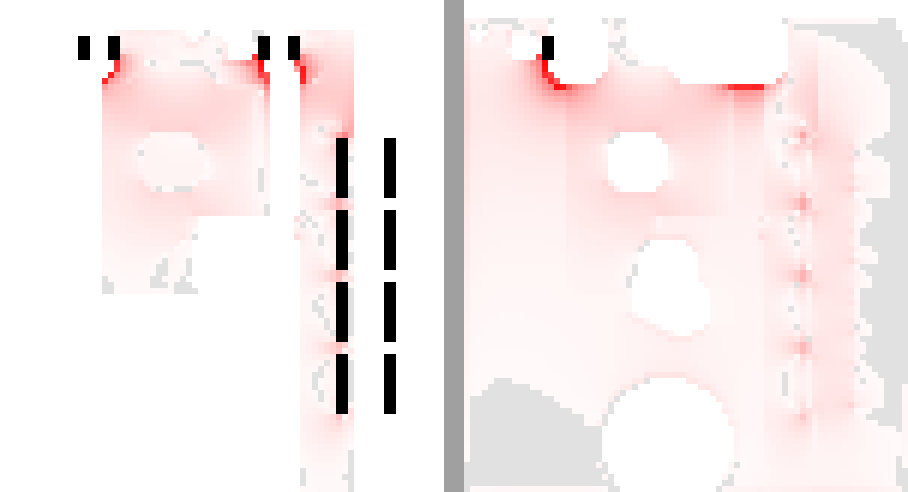
\includegraphics[width=0.92\textwidth]{figures/kicad_maglia_energia_v10.png}
    \caption{revision 1.0: \SI{11.7}{\nano\henry}}\end{subfigure}\\[2mm]
  \begin{subfigure}{\textwidth}\centering
    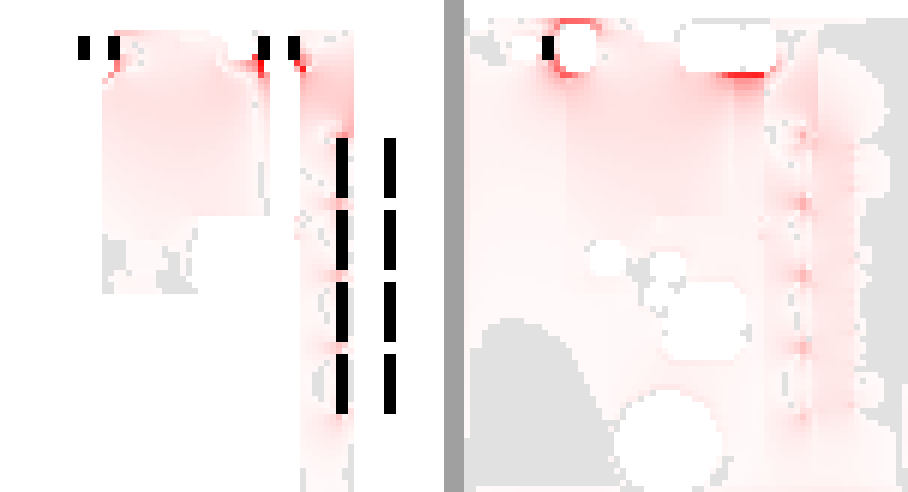
\includegraphics[width=0.92\textwidth]{figures/kicad_maglia_energia_v11.png}
    \caption{revision 1.1, inner-layer clearance \SI{2.25}{\milli\metre}: \SI{7.8}{\nano\henry}}\end{subfigure}
  \caption{Magnetic energy density of the commutation loop of leg~1 at
  \SI{1}{\milli\metre} resolution, L1 on the left, L2 on the right of each
  pair (black: device and capacitor pads; grey: copper carrying little
  energy; same colour scale within each pair). The energy sits at the device
  pins and along the edges of the clearance holes that the negative plane
  leaves around the other pins; smaller holes, less energy.}
  \label{fig:loopenergy}
\end{figure}

\begin{finding}{The inductance is in the clearance holes, not in the plane pair}
The estimate of \cref{tab:loopbudget} was 5 to \SI{10}{\nano\henry}; the
extraction of revision 1.0 gave more, and \cref{fig:loopenergy} shows where. Of the
\SI{12}{\nano\henry}, \SI{8.6}{} are spent in the strip of board under the
device row, and almost all of it along the edges of the holes in the
negative plane. The plane must keep \SI{4.5}{\milli\metre} from the
switching-node and positive-rail pins and from the high-side gate pins,
which on a \SI{5.08}{\milli\metre} pitch opens a hole about
\SI{10}{\milli\metre} wide under each device: the return current has to
drop some \SI{6}{\milli\metre} below the row before it can run under the
outgoing current. With a plane free of holes (not buildable, but a useful
bound) the same copper gives \SI{4.0}{\nano\henry}; the holes cost
\SI{7.7}{\nano\henry}.

The \SI{4.5}{\milli\metre} is a creepage figure for a surface in
pollution degree 2, and it is applied to every layer. Inside the laminate
there is no surface and no pollution: IPC-2221B asks
\SI{0.0025}{\milli\metre\per\volt} above \SI{500}{\volt} for internal
conductors, \SI{2.25}{\milli\metre} at \SI{900}{\volt}~\cite{ipc2221}. Applied
to the inner layers only, it takes the loop from 12 to
\SI{7.8}{\nano\henry}, a third less, with no other change to the copper.
Revision 1.1 adopts it: one rule, for the negative plane against
the other high-voltage nets and the high-side domains on inner layers; the
outer layers keep \SI{4.5}{\milli\metre} and the reinforced barrier is
untouched. Four new cases on the rules test board check exactly that (2 and
\SI{3}{\milli\metre} on L2, \SI{3}{\milli\metre} on L1,
\SI{6}{\milli\metre} to ground on L2).
\end{finding}

\section{Conductor sizing}
\label{sec:conductors}

Two currents have to be carried. The phase conductors carry
\SI{30}{\Arms}; the DC bus carries the input current
%
\begin{equation}
  I_\mathrm{bus} = \frac{P_\mathrm{out} + P_\mathrm{tot}}{\Vdc}
  = \frac{\SI{25.605}{\kilo\watt}}{\SI{800}{\volt}}
  = \SI{32.0}{\ampere},
  \label{eq:ibus}
\end{equation}
%
rounded up to \SI{35}{\ampere} for the ripple superimposed on it.

\begin{table}[htbp]
\centering
\caption{Minimum conductor width, IPC-2221B closed form~\cite{ipc2221},
external layer, \SI{2}{oz} copper.}
\label{tab:widths}
\begin{tabular}{llrr}
\toprule
Conductor & Current & $\Delta T = \SI{20}{\kelvin}$ & $\Delta T = \SI{30}{\kelvin}$ \\
\midrule
Phase  & \SI{30}{\Arms}   & \SI{10.7}{\milli\metre} & \SI{8.4}{\milli\metre} \\
DC bus & \SI{35}{\ampere} & \SI{13.3}{\milli\metre} & \SI{10.4}{\milli\metre} \\
\bottomrule
\end{tabular}
\end{table}

At these currents the conductors are copper pours, not tracks, and the
computed widths serve as a minimum check. Two warning rules flag any
\emph{track} on a bus or phase net narrower than \SI{10.4}{} or
\SI{8.4}{\milli\metre}. Two kinds of connection are exempted by name,
because they carry milliamperes and not the load current: the desaturation
diode's lead to the drain, and the bus-voltage divider around the bus
amplifier, marked by a rule area. Every other narrow track on those nets
still raises the warning, and the frozen board raises none.

\begin{finding}{The width rule checks tracks, and the narrowest conductor is a pour}
The positive DC rail is a single pour of \SI{411}{\centi\metre\squared} on
L1 over the \SI{627}{\centi\metre\squared} negative plane on L2, and the
switching-node pours are never narrower than \SI{13}{\milli\metre}. The
phase pours were measured afterwards, section by section on the filled
copper, because no rule looks at them: they are at least
\SI{10.5}{\milli\metre} wide from the shunt to the terminal, but
about \SI{8}{\milli\metre} for some \SI{4}{\milli\metre} just below
the shunt pad, where the pour of the switching node takes the rest of the row.

That is below the \SI{8.4}{\milli\metre} of the \SI{30}{\kelvin} column; by
the same closed form a long conductor that narrow would rise by about
\SI{33}{\kelvin} instead of \SI{30}{}. Revision 1.1 removes the
neck without moving a part: a second phase pour on L6, the full
\SI{22}{\milli\metre} of the phase area wide because the switching node has
no copper on that layer, stitched to L1 by twenty vias in four rows and
collected at the phase terminal, which is through-hole. The narrowest
section becomes 8 plus \SI{22}{\milli\metre} of \SI{2}{oz} copper. The pour
starts \SI{5.5}{\milli\metre} below the shunt centre, so the phase current
on L6 does not run under the Kelvin loop of the measurement. Widening the
L1 pour instead would have meant relaxing the \SI{4.5}{\milli\metre}
between switching node and phase, two nets a few millivolts apart in
operation but not if the shunt fails open. The lesson is about the check
rather than the copper: a width rule on tracks says nothing about pours,
and a board whose power path is all pours needs its sections measured.
\end{finding}

The IPC-2152 charts~\cite{ipc2152} supersede the closed form and were not
available (\cref{app:assumptions}, A.15).

\section{Common-mode and EMC}
\label{sec:emc}

Emissions can only be measured against CISPR 25~\cite{cispr25} on a built
board; what the layout can do is keep the common-mode currents short and
known. The switching node moves the full bus at \SI{31}{\volt\per\nano\second}
between \SI{10}{} and \SI{90}{\percent} of the steeper edge, in the
double-pulse simulation at \SI{950}{\volt} and \SI{60}{\ampere}
(\cref{sec:kelvin}), and every capacitance to chassis carries a current
proportional to that slope.

\begin{table}[htbp]
\centering
\caption{Capacitance from the switching nodes to chassis.}
\label{tab:cmcap}
\begin{tabular}{lrr}
\toprule
Source & Capacitance & Peak current \\
\midrule
Isolation barriers of the auxiliary circuits & \SI{25.5}{\pico\farad} & \SI{0.80}{\ampere} \\
\textbf{Insulating pads, three low-side devices} & \SI{131}{\pico\farad} & \SI{4.11}{\ampere} \\
Motor and cable, assumed & \SI{1}{\nano\farad} & \SI{31}{\ampere} \\
\bottomrule
\end{tabular}
\end{table}

The middle row was missing from the earlier analysis. The pad is an
insulator and a capacitor at once: alumina of relative permittivity
\num{9.8}, \SI{0.63}{\milli\metre} thick, under a
\SI{15.9}{}$\times$\SI{20}{\milli\metre} tab gives \SI{43.8}{\pico\farad} per
device. Only three of the six count, because the tab is the \emph{drain}: on
the high side that is the DC-positive rail, which does not move, and on the
low side it is the switching node, which does. The aluminium nitride
adopted in \cref{sec:coolalt} has a permittivity of about 
\num{8.8}, ten
percent less: the alumina figures are kept here as the upper bound.

The conclusion survives, since the motor cable still dominates and effort
belongs in the screen termination and the Y-capacitors, but by a factor of
\num{7.6} rather than \num{40}, and second place belongs to the pads rather
than to the driver barriers. If on-board common-mode current had to be
reduced, the lever would be a \emph{thicker} pad, not a lower-capacitance
driver: halving the thickness doubles this term to
\SI{263}{\pico\farad} while halving $\Rthcs$. Pad \emph{area} does not enter
it at all, since the electrode is the tab and the fringing field decays over
a distance of order the thickness, and the \SI{8.4}{\milli\metre} overhang
is already thirteen times that.

\subsection{A first estimate against CISPR 25}
\label{sec:emcest}

Emissions are measured, not computed; but the two sources that drive the
conducted part are known well enough to say, before a board exists, how far
from a limit it will start and what filter it will need. The estimate works
on a circuit model of the measurement set-up of CISPR~25~\cite{cispr25}: the
\SI{5}{\micro\henry}/\SI{50}{\ohm} artificial network on each DC line, a
metre of harness, and the impedances this report has already computed.
%
\begin{itemize}
  \item The sources, simulated with the real modulation over one
        fundamental period: the common-mode voltage of the three legs and the
        input current of the bridge, with the edges of the double-pulse
        simulation. Two operating points: rated, and locked rotor, where the
        three duty cycles are almost equal, the legs switch together and the
        common-mode voltage is the worst it can be.
  \item The paths: for the common mode, the capacitances to chassis of
        \cref{tab:cmcap} and the two Y-capacitors that return the current to
        the bus; for the differential mode, the commutation ceramics, the
        films behind the plane inductance, and the harness.
  \item The receiver: a \SI{9}{\kilo\hertz} Gaussian filter and a peak
        detector, compared with the voltage-method peak limits of the
        broadcast bands, class~3 as reference. These are the low-voltage
        limits; the edition and class for the high-voltage lines remain to be
        fixed (A.19), so the comparison says how large the gap is, not whether
        a test passes.
\end{itemize}

\begin{table}[htbp]
\centering
\caption{Estimated conducted emission above the CISPR~25 class~3 peak limit,
worst operating point, by band (dB; negative is below the limit).}
\label{tab:emcest}
\small
\begin{tabular}{lrrrr}
\toprule
 & LW & MW & SW & CB \\
Band [\si{\mega\hertz}] & 0.15--0.3 & 0.53--1.8 & 5.9--6.2 & 26--28 \\
\midrule
Common mode, board as frozen & $+19$ & $+56$ & $+35$ & $+8$ \\
Differential mode, board as frozen & $-3$ & $+33$ & $-1$ & $-13$ \\
Common mode, with the input filter & $-9$ & $-3$ & $-3$ & $-7$ \\
Differential mode, with the input filter & $-34$ & $-33$ & $-69$ & $-80$ \\
\bottomrule
\end{tabular}
\end{table}

\begin{figure}[htbp]
\centering
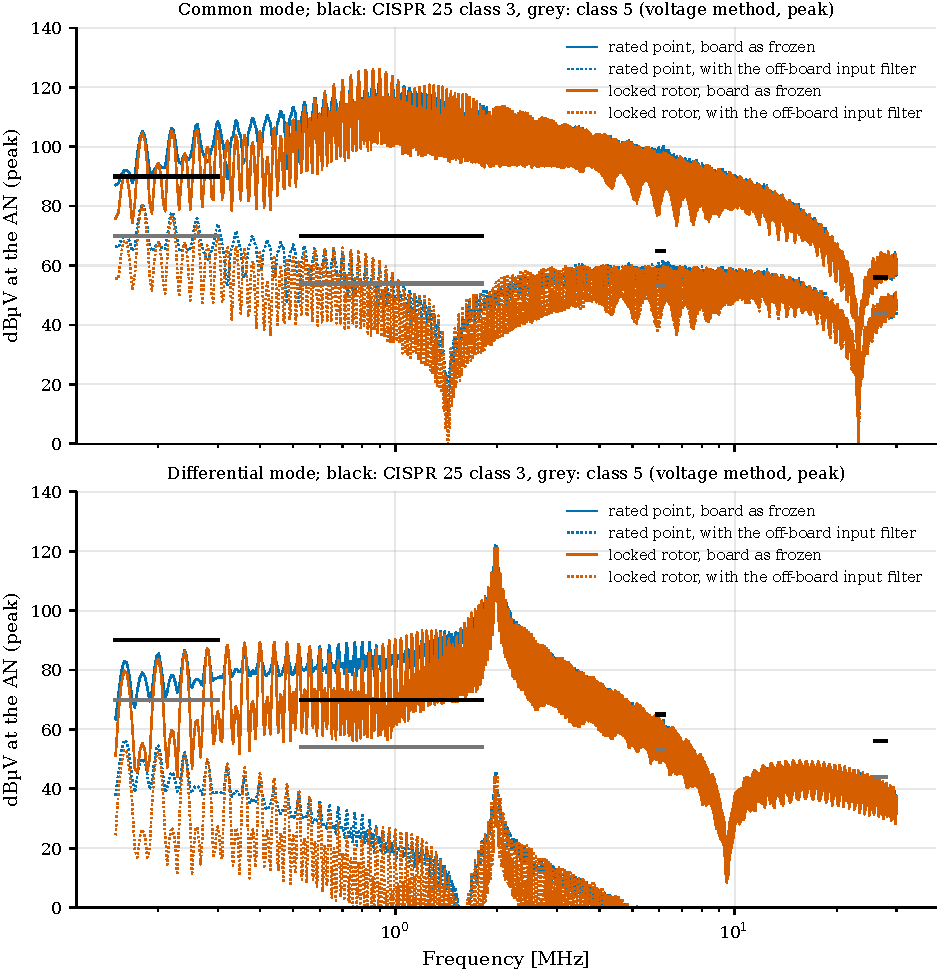
\includegraphics[width=\textwidth]{emc_emc_condotte.pdf}
\caption{Estimated conducted emission at the artificial network, common and
differential mode, rated point and locked rotor, without and with the
off-board input filter of \cref{tab:emcfilter}; class~3 (black) and class~5
(grey) peak limits in the broadcast bands.}
\label{fig:emcest}
\end{figure}

\begin{finding}{The board as frozen needs an input filter, as every unfiltered inverter does}
Without a filter the common mode exceeds class~3 by up to \SI{56}{\decibel}
in the medium-wave band, and the differential mode by \SI{33}{\decibel}. The
numbers are large but not surprising: an \SI{800}{\volt} bridge switching
at \SI{31}{\volt\per\nano\second} into a nanofarad of motor capacitance is a
strong source, and the two \SI{4.7}{\nano\farad} Y-capacitors are the only
return path that does not cross the measurement. The differential-mode
excess sits at the top of the medium-wave band because the film--ceramic
resonance of \cref{sec:complife}, at \SI{2.0}{\mega\hertz}, is just above it.
\end{finding}

\paragraph{The filter, and where it goes.} The model then sizes the filter,
and the first thing it shows is that none of it needs to be on this
board. An input filter between the battery and the DC terminals J101--J102,
in its own compartment of the inverter housing, does the whole job; that is
also where traction inverters usually carry it, on the DC busbars.
%
\begin{itemize}
  \item Common mode: two KEMET SCF39XV-400-2R2B005JH in series,
        nanocrystalline, \SI{0.62}{\milli\henry} each, \SI{40}{\ampere},
        rated \SI{1000}{\volt} AC or DC and qualified to AEC-Q200. One alone
        leaves \SI{3}{\decibel} over the limit in the medium-wave band; two
        give \SI{1.24}{\milli\henry}. Inductance is not the only figure:
        above its self-resonance a choke is a capacitor, and the residual in
        the short-wave and CB bands is set by that capacitance. With
        \SI{20}{\pico\farad} even \SI{2}{\milli\henry} stays \SI{1}{\decibel} above the limit;
        the estimate assumes \SI{10}{\pico\farad} for the pair, which a
        sectored winding reaches, and the choke's datasheet must confirm it.
  \item Differential mode: no separate inductor. The leakage of the
        common-mode chokes, about \SI{1}{\percent} of their inductance, with
        a \SI{1}{\micro\farad} film X-capacitor on the battery side, forms an
        LC filter. An inductor alone works poorly against the
        \SI{100}{\ohm} of the network (\SI{20}{\micro\henry} still leaves
        \SI{18}{\decibel}), while the LC brings the differential mode
        \SI{33}{\decibel} below the limit.
  \item No damper. An RC network across the bus, tuned to the
        film--ceramic resonance, removes \SI{12}{\decibel} on its own; with
        the X-capacitor in place it adds less than \SI{1}{\decibel}, and it
        would have been the only part of the filter on the board. It is
        left out.
\end{itemize}

\begin{table}[htbp]
\centering
\caption{Input EMI filter, outside the board, between battery and the DC
terminals.}
\label{tab:emcfilter}
\small
\begin{tabularx}{\textwidth}{lYY}
\toprule
Part & Choice & Requirement it meets \\
\midrule
CM choke, two in series & KEMET SCF39XV-400-2R2B005JH, \SI{0.62}{\milli\henry}, \SI{40}{\ampere}, \SI{1000}{\volt}, AEC-Q200 &
  \SI{1.24}{\milli\henry} in total; self-capacitance $\leq\SI{10}{\pico\farad}$; bus current \SI{32}{\ampere} with ripple \\
X-capacitor & \SI{1}{\micro\farad}, \SI{1100}{\volt} DC film, AEC-Q200 (Panasonic ECW-FG class) & battery side of the chokes \\
Y-capacitors & the two \SI{4.7}{\nano\farad} on the board & inverter side of the chokes, as they are \\
Cables & shielded DC and motor cables, \SI{360}{\degree} shield termination at the housing &
  the motor capacitance returns through the shield, not through the network \\
\bottomrule
\end{tabularx}
\end{table}

With the filter the estimate is inside class~3 in every band, by at least
\SI{3}{\decibel} (\cref{tab:emcest}). That margin is thin against the
accuracy of an estimate, and the medium-wave band, where the inductance runs
out first, is the one to watch; a third choke is the obvious reserve. Two
side effects are welcome. The leakage of the chokes, about
\SI{12}{\micro\henry}, sits between the battery and the DC-link and meets
requirement R11 from inside the inverter: the source--capacitor resonance of
\cref{sec:dclink} moves to about \SI{3}{\kilo\hertz}, far below the
switching harmonics. And the chokes dissipate about \SI{3}{\watt} at full
current, in the filter compartment and not on the board.

The estimate does not cover what only a built board shows: radiated
emission, coupling between the switching nodes and the harness, the actual
shield termination, and anything above \SI{30}{\mega\hertz}. It does say
how large the filter is, that it fits outside the frozen board, and what it
costs: about \SI{140}{}~EUR on a prototype (\cref{app:bom}).

\section{Insulation coordination}
\label{sec:insulation}

The requirements quoted below come from a third-party calculator that
implements a stored subset of IEC 60664-1~\cite{standardclarity}, not from
the text of the standard~\cite{iec60664}, which was not available. This is a
secondary source: published, reproducible and parameter-addressable, but not
the standard itself, and it describes itself as a reference estimate. Every
case cited here is reproducible from the permalink given in the reference.

It was used to check nine values that had previously been quoted from
memory (five creepage rows, two clearance rows, the reinforced doubling rule
and the pollution-degree floor), and all nine agree to the digit.
That is reassuring about the memory and says nothing about the calculator's
own coverage; the standard is still to be read before release
(\cref{app:assumptions}).

\paragraph{\SI{900}{\volt} is not a row of the tables.} The creepage table
of IEC 60664-1 lists \SI{800}{} and \SI{1000}{\volt}; every creepage value at
\SI{900}{\volt} in this chapter is a \emph{linear interpolation} between
the two, which is what the calculator does and states that it
does~\cite{standardclarity}, rounded up to the next \SI{0.1}{\milli\metre}.
Clearance is treated differently and needs no interpolation at all: it is
selected by rated impulse voltage in discrete steps, and \SI{2.5}{\kilo\volt}
is a row (\SI{1.5}{\milli\metre}; \SI{3.00}{\milli\metre} for reinforced
insulation, taken one impulse step higher, at \SI{4}{\kilo\volt}).
Whether the standard permits interpolating creepage is to be confirmed on
its text. If it did not, the \SI{1000}{\volt} row would apply: in pollution
degree 1, which is the design basis, the drain--source gap would pass by
\SI{1}{\percent} (\SI{3.24}{} against \SI{3.2}{\milli\metre}) and every
other barrier would keep its margin; the pollution-degree-2 checks of
\cref{tab:pd2robust} would each lose \SI{0.5}{} to \SI{1}{\milli\metre}.

\subsection{What the package leaves}

The worst pair is drain to source on a single device, and its separation is
fixed by the package: pads \SI{1.84}{\milli\metre} wide on a
\SI{5.08}{\milli\metre} pitch leave \SI{3.24}{\milli\metre} of bare laminate
at the full bus voltage. The other close pair, at \SI{0.70}{\milli\metre}, is
between source, Kelvin source and gate, which see the gate voltage and not
the bus.

\begin{table}[htbp]
\centering
\caption{Creepage required at the \SI{900}{\volt} working voltage
($V_\mathrm{max,cont}$, \cref{tab:vhierarchy}) against the
\SI{3.24}{\milli\metre} available.}
\label{tab:creepage}
\begin{tabular}{lrrl}
\toprule
Condition & Required & Margin & \\
\midrule
\textbf{Pollution degree 1}, coated & \textbf{\SI{2.80}{\milli\metre}} & $+\SI{16}{\percent}$ & \textbf{passes} \\
PD2, material group I (CTI $\geq$ \num{600}) & \SI{4.50}{\milli\metre} & $-\SI{39}{\percent}$ & fails \\
PD2, material group II & \SI{6.35}{\milli\metre} & $-\SI{96}{\percent}$ & fails \\
PD2, material group IIIa (ordinary FR-4) & \SI{9.00}{\milli\metre} & $-\SI{178}{\percent}$ & fails \\
\bottomrule
\end{tabular}
\end{table}

\subsection{Clearance, and the rule that couples it to creepage}
\label{sec:clearance}

Creepage may not be smaller than clearance. Clearance in turn does not follow
from the working voltage but from the assumed \emph{rated impulse withstand},
so an assumption about impulse can raise the required creepage above the
table value, and the next subsection works out what that means for this
board.

\begin{table}[htbp]
\centering
\caption{Rated impulse, clearance, and the creepage that results in pollution
degree 1, against the \SI{3.24}{\milli\metre} the package leaves.}
\label{tab:impulse}
\begin{tabular}{lrrl}
\toprule
Rated impulse & Clearance & Creepage (PD1) & Margin on \SI{3.24}{\milli\metre} \\
\midrule
\SI{1.5}{\kilo\volt} & \SI{0.50}{\milli\metre} & \SI{2.80}{\milli\metre} & $+\SI{16}{\percent}$ \\
\textbf{\SI{2.5}{\kilo\volt}} (selected) & \SI{1.50}{\milli\metre} & \SI{2.80}{\milli\metre} & $+\SI{16}{\percent}$ \\
\SI{4}{\kilo\volt} & \SI{3.00}{\milli\metre} & \SI{3.00}{\milli\metre} & $+\SI{8}{\percent}$ \\
\SI{6}{\kilo\volt} & \SI{5.50}{\milli\metre} & \SI{5.50}{\milli\metre} & $-\SI{41}{\percent}$: fails \\
\bottomrule
\end{tabular}
\end{table}

At the selected level the air gap (\SI{1.50}{\milli\metre} required against
\SI{3.24}{\milli\metre} available) does not constrain the design, and the
surface path governs, which is what the coating addresses. Clearance stays below creepage only as long as the impulse assumption of
\cref{sec:ovc} holds. Above \SI{4}{\kilo\volt} clearance
becomes the quantity that sets creepage, and the design does not survive
\SI{6}{\kilo\volt}.

\subsection{Overvoltage category does not apply here}
\label{sec:ovc}

IEC 60664-1 coordinates insulation for equipment \emph{within low-voltage
supply systems}. Its rated-impulse table is indexed by the nominal voltage of
the supply system and by the overvoltage category, and the category encodes
one thing: how much the distribution network attenuates a lightning or
switching transient before it reaches the equipment.

This inverter is fed from a traction battery, and the high-voltage system
floats with respect to chassis. During driving it is connected to no
distribution network at all.

During charging it is. The contactors are \emph{closed} while charging,
since that is how the energy reaches the pack, so a conductive path from the inlet to the DC bus exists, with the
inverter sitting on it. What interrupts the mains transient is not the
contactors but the galvanic isolation of the charging equipment: the
high-frequency transformer of the on-board charger in AC charging, or of the
off-board station in DC charging. That is equipment outside this perimeter,
so it becomes a requirement on the system (R10 of \cref{tab:sysreq}) rather
than an assumption buried in a clearance table.

Whether it is normatively guaranteed is less clear. The governing
documents are ISO 17409~\cite{iso17409} on the vehicle side and
IEC 61851-23~\cite{iec6185123} for DC charging stations; neither text was
available here. What is known of their structure settles the question in the
negative: IEC 61851-23 distinguishes isolated from non-isolated DC charging
stations and imposes additional protective measures on the latter, so
galvanic isolation is \emph{not} universally mandated. It is an architecture
assumption, and it is recorded as one.

With that assumption standing, there is no physical path by which a
\SI{6}{\kilo\volt} mains-borne impulse reaches the drain--source gap of a
device, and applying category II would transfer a mains assumption to a
system separated from the mains by a transformer. Without it, the bus is
galvanically tied to the grid while charging, the category applies again, and
the \SI{2.5}{\kilo\volt} declared here would not help: that is not a
transient this board can absorb but a different normative domain, to be
mitigated at the charge inlet rather than on this board.

\begin{finding}{Overvoltage category II would have failed the board}
Selecting the \SI{1000}{\volt} supply band with overvoltage category
II, the combination an engineer trained on mains-connected equipment reaches
for, gives a \SI{6}{\kilo\volt} rated impulse, \SI{5.50}{\milli\metre} of
clearance, and therefore \SI{5.50}{\milli\metre} of required creepage against
\SI{3.24}{\milli\metre} available. The board would fail by \SI{41}{\percent},
and no coating recovers it.

The design survives because the overvoltage category is a category error for
a battery system, not because of a margin. Since that reason sounds fragile,
the room it leaves matters: the design passes up to and including a \SI{4}{\kilo\volt} rated impulse, which
is what category~I on a \SI{1000}{\volt} system would give. It fails only at
category II or worse.
\end{finding}

What replaces the category is the transient that exists on the board, which is
generated inside the converter and has been simulated rather than assumed:
at the \SI{950}{\volt} overvoltage trip and the \SI{60}{\ampere} overload
trip the die sees \SI{1073.5}{\volt} with the \SI{20}{\nano\henry} layout
limit and \SI{1148}{\volt} even at \SI{50}{\nano\henry}, two and a half times
the limit (\cref{tab:overshoot}).

\begin{finding}{Opening a contactor is worth five volts, not kilovolts}
The step from \SI{1.5}{} to \SI{2.5}{\kilo\volt} was originally justified by
a contactor opening into an inductive high-voltage harness, an event that had
never been estimated. Estimating it changes the argument.

Two \SI{50}{\milli\metre\squared} conductors \SI{30}{\milli\metre} apart give
$(\mu_0/\pi)\ln(d/r) = \SI{0.72}{\micro\henry\per\metre}$, so a
\SI{3}{\metre} harness is \SI{2.16}{\micro\henry}. What matters next is the
topology: the DC-link capacitor sits on the \emph{inverter} side of that
harness, so when the contactor opens the harness current continues into
\SI{200}{\micro\farad}. The circuit impedance is
$\sqrt{L/C} = \SI{0.104}{\ohm}$ and the overvoltage is $I\sqrt{L/C}$:
\SI{3.6}{\volt} at \SI{35}{\ampere}, \SI{10.4}{\volt} at \SI{100}{\ampere},
\SI{52}{\volt} if a fuse interrupted \SI{500}{\ampere}. Reaching
\SI{2.5}{\kilo\volt} would take \SI{24}{\kilo\ampere}.

The DC-link capacitor is a formidable clamp for anything arriving along the
harness, and the dominant transient on this board remains the one the board
generates itself.
\end{finding}

\SI{2.5}{\kilo\volt} is declared even so, one step above the
\SI{1.5}{\kilo\volt} that would cover the simulated worst case. The reason is
not the external events, which are now quantified at tens of volts, but what
cannot be quantified: electrostatic discharge at the high-voltage connector
during service, lightning coupling to the vehicle, anything this model does
not contain. It costs nothing, because creepage remains the binding quantity
at \SI{2.80}{\milli\metre} either way, so the figure is \emph{abundant rather
than marginal}: \num{2.2} times the worst internal case and \num{48} times
the worst external event estimated.

\subsection{Two air paths the design rule check cannot see}

Clearance is a distance through air, and two of the air paths that matter run
outside the board copper the design rule check measures.

The tab of the TO-247 package \emph{is} the drain, at up to \SI{900}{\volt}, and it
is clamped against a cold plate at chassis potential. The insulating pad
handles the solid insulation; what had never been dimensioned is the surface
path around the \emph{edge} of the pad, which is a reinforced barrier.

\begin{finding}{The pad is outside the board, so it inherits nothing from the
coating}
Every other distance in this design is qualified in pollution degree 1
because the board is conformally coated. The pad is not on the board: it sits
between the package tab and the cold plate, and that surface is not coated.
Its pollution degree depends on the sealing of the housing (a mechanical
part outside this perimeter), not on our coating process. The two are
independent assumptions, and treating them as one was an error.

The source used here says as much: coating or sealing does not automatically
reduce the pollution degree, and any reduction depends on the protection
method applied~\cite{standardclarity}.
\end{finding}

\begin{table}[htbp]
\centering
\caption{Insulating pad sized by the creepage around its edge. Reinforced
barrier at \SI{900}{\volt}; path available is the overhang plus the
\SI{0.63}{\milli\metre} pad thickness; tab \SI{15.9}{}$\times$\SI{20}{\milli\metre}.}
\label{tab:pad}
\begin{tabular}{lrrl}
\toprule
Microenvironment at the pad & Creepage & Overhang & Pad \\
\midrule
PD1, sealed housing & \SI{5.60}{\milli\metre} & \SI{4.97}{\milli\metre} & \SI{26}{}$\times$\SI{30}{\milli\metre} \\
\textbf{PD2, material group I} (selected) & \SI{9.00}{\milli\metre} & \SI{8.37}{\milli\metre} & \textbf{\SI{33}{}$\times$\SI{37}{\milli\metre}} \\
PD2, material group II & \SI{12.70}{\milli\metre} & \SI{12.07}{\milli\metre} & \SI{41}{}$\times$\SI{45}{\milli\metre} \\
\bottomrule
\end{tabular}
\end{table}

Pollution degree 2 is chosen, and the housing assumption is
dropped. Most automotive housings carry a pressure-equalisation membrane,
which means they breathe and therefore condense; the standard places
occasional condensation explicitly inside pollution degree 2. Buying
independence from a system-level assumption costs \SI{57}{\percent} more pad
area on a component worth a few euro. This is the only point in the whole
insulation coordination where an assumption was \emph{removed} rather than
declared.

The ceramic itself is assigned material group I, which a pad datasheet
stating CTI $\geq \SI{600}{\volt}$ would confirm. Neither alumina nor the
aluminium nitride adopted in \cref{sec:coolalt} tracks, and
the standard is understood to exempt non-tracking inorganic materials from
requiring creepage greater than clearance, which would give
\SI{3.00}{\milli\metre} instead of \SI{9.00}{\milli\metre}. That exemption is
\emph{not} taken: the secondary source available does not implement it, and
the path runs over ceramic veiled in thermal grease, which is organic.

A catalogue part sold as a TO-247 pad is typically
\SI{20}{}$\times$\SI{25}{\milli\metre}, less than a third of the required
area. The pad had been selected on thermal resistance alone
(\cref{tab:rthcs}), where its size never appears. \Cref{tab:pad} sizes a pad
standing on its own; on the cooling rail of \cref{sec:mechanics} the strip
is \SI{35.5}{\milli\metre} tall, and the creepage below the tab is obtained by
raising the rail rather than by extending the ceramic, which gives
\SI{10.1}{\milli\metre} around the edge (\cref{fig:mechsection}).

The thermal chain does not move. Heat enters through the tab and spreads at roughly
\SI{45}{\degree} as it crosses the pad, so the flux widens by about one pad
thickness (\SI{0.63}{\milli\metre}) per side. The overhang is
\SI{8.4}{\milli\metre}, thirteen times that, and therefore lies entirely
outside the spreading cone: it carries no heat. Adding ceramic around the
loaded area cannot increase $\Rthcs$; it can only add a weak parallel path.
The pad's size therefore changes no temperature in this report; its
thermal resistance is set by the material and the interfaces
(\cref{sec:coolalt}).

\begin{finding}{A screw through the tab would short the barrier the pad
creates}
The TO-247 has a mounting hole in its tab, and the tab is the drain at
up to \SI{900}{\volt}. A metal screw passing through it into the cold plate
reduces the creepage path from \SI{9}{\milli\metre} to zero. Clip mounting on the
plastic body is therefore selected, which also gives the uniform pressure
that makes $\Rthcs$ reproducible. If a screw were required for mechanical
reasons, an insulating shoulder bushing and washer would be mandatory
components.
\end{finding}

The cold plate itself, its screws and the surrounding structure are at
chassis potential and sit millimetres from the board, but they are not nets
in the PCB file and no rule can check them. A mechanical clearance of
\SI{5.0}{\milli\metre} from any high-voltage copper is specified, above the
\SI{3.00}{\milli\metre} the standard asks, because this dimension lives in an
assembly with mechanical tolerances rather than in a photoplot.

\begin{finding}{Conformal coating is part of the design}
Conformal coating over the high-voltage area brings the pollution degree from
2 to 1 and the requirement from \SI{9.00}{} to \SI{2.80}{\milli\metre}, a
\SI{69}{\percent} reduction that turns a \SI{178}{\percent} shortfall into a
\SI{16}{\percent} margin. Every insulation distance in this design, the
reinforced barrier included, depends on it.

Without the coating the board is \emph{unbuildable with this device}: \SI{9.00}{\milli\metre} would be
required where the package offers \SI{3.24}{\milli\metre}, and no layout can
recover the difference. The design-rule check cannot see this, since the board
passes either way, so the condition is stated at the head of the rules file
and on the fabrication drawing.
\end{finding}

The reinforced barrier to the control side is set at \SI{8}{\milli\metre},
which is what the components themselves
provide~\cite{ti_ucc21750,ti_amc1302}. Read against IEC 60664-1, where
reinforced insulation requires twice the basic creepage, that is
\SI{5.60}{\milli\metre} in pollution degree 1 and \SI{18}{\milli\metre} in
pollution degree 2 on ordinary FR-4, at \SI{900}{\volt}. The adopted figure
therefore has \SI{43}{\percent} of margin under the coating assumption and
none without it. Saying that this
barrier is ``guaranteed by the components'' is true of the component body and
false of the copper around it.

\subsection{Laminate material group}

The certified creepage of an isolator and the CTI of its body describe the
component. The path that has to be qualified runs on the \emph{laminate},
which is a different material and is ordinarily material group IIIa. The
laminate is therefore specified in its own right, at CTI
$\geq\SI{600}{\volt}$, material group I.

On its own this does not save the drain--source pair (\SI{4.50}{\milli\metre}
required against \SI{3.24}{\milli\metre} available), so it is not an
alternative to the coating. It is a second line of defence, because coating
voids are a known process defect: on ordinary FR-4 a void takes the margin to
$-\SI{178}{\percent}$, on a group I laminate to $-\SI{39}{\percent}$. It is
also the only defence at the board edge, which a coating does not reliably
reach.

\subsection{The board edge, and solid insulation}

Two more paths need checking: around the board edge, and through the solid
insulation between the planes.

Between the DC-positive plane on L1 and the DC-negative plane on L2 the
\SI{0.10}{\milli\metre} prepreg is \emph{solid} insulation, but a second path
exists around the side of the board. Its length is the sum of the two plane
setbacks plus the dielectric. A routed edge is not reliably coated and is
treated as pollution degree 2, where the group I laminate requires
\SI{4.50}{\milli\metre} at \SI{900}{\volt}: the \SI{2.0}{\milli\metre}
setback of the first version gave \SI{4.10}{\milli\metre} and no longer
passes. The rule is now \SI{2.25}{\milli\metre} per plane,
\SI{4.60}{\milli\metre} in all.

The solid insulation itself carries up to \SI{900}{\volt} across
\SI{0.10}{\milli\metre}, a field of \SI{9}{\kilo\volt\per\milli\metre}
against a laminate strength of the order of \SI{30}{}--\SI{40}{\kilo\volt\per\milli\metre}.
It is functional insulation, so no minimum thickness applies (the
\SI{0.4}{\milli\metre} minimum is a reinforced-insulation rule), but this is
the thinnest margin in the design and it cannot be inspected. A
layer-to-layer dielectric withstand test at \SI{2}{\kilo\volt} for one minute
is added to the fabrication drawing, which replaces the assumption with a
measurement.

\subsection{What fails if the coating has a void}

The pad raises a more general question: which barriers survive in pollution
degree 2? With the material group I laminate specified in \cref{sec:insulation}:

\begin{table}[htbp]
\centering
\caption{Barriers against the pollution degree 2 requirement, material group I laminate.}
\label{tab:pd2robust}
\begin{tabular}{lrrl}
\toprule
Barrier & Adopted & Required & Survives? \\
\midrule
Reinforced, HV to control, board copper & \SI{9.5}{\milli\metre} & \SI{9.00}{\milli\metre} & \textbf{yes} \\
Reinforced, isolators: board, around the slot & $\geq\SI{9.5}{\milli\metre}$ & \SI{9.00}{\milli\metre} & \textbf{yes} \\
Reinforced, isolators: package surface & \SI{8.0}{}/\SI{8.5}{\milli\metre} & \SI{9.00}{\milli\metre} & no$^a$ \\
Reinforced, HV to chassis & \SI{9.5}{\milli\metre} & \SI{9.00}{\milli\metre} & \textbf{yes} \\
Functional, HV nodes on the board & \SI{4.5}{\milli\metre} & \SI{4.50}{\milli\metre} & equal$^b$ \\
Functional, drain--source in the package & \SI{3.24}{\milli\metre} & \SI{4.50}{\milli\metre} & no \\
\bottomrule
\multicolumn{4}{l}{\footnotesize $^a$ drivers/amplifiers; a property of the certified component, \cref{sec:isoslot}.} \\
\multicolumn{4}{l}{\footnotesize $^b$ exact equality, declared: see the text below the table.}
\end{tabular}
\end{table}

\begin{finding}{At \SI{900}{\volt} a coating void can reach the reinforced barrier}
At \SI{800}{\volt} the \SI{8}{\milli\metre} taken from the isolator bodies
coincided exactly with what pollution degree 2 requires of a reinforced
barrier on a group I laminate, and the safety barriers held with no coating
at all. At the \SI{900}{\volt} working voltage the requirement is
\SI{9.0}{\milli\metre}. The board copper can follow, and the rule is set at
\SI{9.5}{\milli\metre}; under the isolators a slot takes the board path out
of the question (\cref{sec:isoslot}), and what remains is the surface of the
isolator packages themselves, \SI{8.0}{} and \SI{8.5}{\milli\metre}.

Elsewhere what fails is functional insulation, and, once the board rule is
raised to \SI{4.5}{\milli\metre}, only inside the six small areas occupied
by the device pads, where the \SI{5.08}{\milli\metre} lead pitch leaves
\SI{3.24}{\milli\metre} that no rule can widen.

Raising the board rule costs nothing, because lateral separation does not
open the commutation loop, which closes vertically. The design-rule file
carries the exception as a named area over the pad rows rather than lowering
the threshold everywhere, so that a violation anywhere else is still
reported.
\end{finding}

\paragraph{Two equalities, treated differently.} In the first version of
\cref{tab:pd2robust} two barriers met their requirement exactly, and a
margin of zero protects nothing: the drawn gap survives only if every
fabrication tolerance breaks favourably, and the requirement itself is an
interpolation. The reinforced rules are raised from \SI{9.0}{} to
\SI{9.5}{\milli\metre}, because their failure is an electric-shock hazard
and the half millimetre costs only board area. The functional rule
stays at \SI{4.5}{\milli\metre} and is declared as an exact equality in
pollution degree 2: its design basis is pollution degree 1, where the
requirement is \SI{2.80}{\milli\metre} and the margin \SI{61}{\percent};
the pollution-degree-2 row is a check of what a coating void would do, and
its failure is a functional one, not a safety one. Raising it would buy
robustness against a double fault (a void \emph{and} an adverse
tolerance) at the price of loop area around the power stage.

\subsection{Why milling a slot was rejected}

A through slot between the drain and source pads would lengthen the surface
path without touching the pitch, and it was considered. It was rejected
because a through slot cuts L1 \emph{and} L2, forcing the return current to
travel around it instead of directly beneath the outgoing current. By
\cref{eq:planepair} that term is proportional to the separation between go
and return, so a detour of a few millimetres takes the plane pair from
\SI{0.19}{\nano\henry} to between \SI{6}{} and \SI{23}{\nano\henry}, the
whole board-attributable budget of \cref{tab:loopbudget}, spent to solve a
problem the coating solves for nothing. The slot would also have to be long
to be effective, since the copper here is a \SI{10.4}{\milli\metre} pour
rather than a track, and a milled wall is not reliably coated in any case.

This is the one place where the insulation constraint and the commutation
loop conflict; elsewhere they do not.
The loop closes \emph{vertically} through \SI{0.10}{\milli\metre} of prepreg
while creepage is measured \emph{laterally} along a surface, so widening a
lateral gap does not open the loop. The two devices of a leg are the most
extreme case: the high-side source and the low-side drain are the same net,
so there is no insulation requirement between them at all and they can be
placed as close as the cold plate allows.

\subsection{The slot that is made: under the isolators}
\label{sec:isoslot}

The slot rejected in the previous subsection sat between drain and source,
inside the commutation loop. A slot under each of the seven drivers and four
isolated amplifiers is a different object, and it is made. The two cases
differ in the three respects that decided the first:

\begin{table}[htbp]
\centering
\caption{The two slots against the criteria that decide them.}
\label{tab:slotcompare}
\small
\begin{tabularx}{\textwidth}{lYY}
\toprule
 & Drain--source slot (rejected) & Isolator slot (adopted) \\
\midrule
Barrier & functional & \textbf{reinforced} \\
Position & inside the commutation loop: cuts L1 and L2 & outside every current path:
  no net crosses an isolation barrier, so nothing crosses the slot \\
Failure it prevents & functional (a flashover between two HV nodes) &
  \textbf{safety} (high voltage reaching the control side) \\
Cost & \SIrange{6}{23}{\nano\henry} of loop inductance & board area and a routing
  operation \\
\bottomrule
\end{tabularx}
\end{table}

\paragraph{How the standard counts a through slot.} A groove or slot
counts in the creepage path only if it is at least $X$ wide: \SI{0.25}{},
\SI{1.0}{} and \SI{1.5}{\milli\metre} in pollution degrees 1, 2 and 3,
narrower grooves being bridged as if absent (IEC 60664-1, as reported in~\cite{ti_slup419}). A \emph{through}
slot does not lengthen the surface path, it interrupts it: there is no
surface across it, so the creepage path has to go around its ends, and the
air gap across it becomes a clearance. Two consequences follow. The
clearance to meet across the slot is the reinforced one, \SI{3.00}{\milli\metre}
at the \SI{4}{\kilo\volt} step, not the \SI{1.5}{\milli\metre} of basic
insulation; it is met anyway, because the air path between the pin rows is
unchanged at \SI{8.1}{\milli\metre} or more. And the slot must be long
enough that the path around its ends meets the creepage rule. A blind
groove would count by its contour instead, but on a six-layer board it
would expose inner copper; a through slot is the standard routing
operation and the one specified.

\paragraph{The footprint was wrong before the slot was.} Sizing the slot
required the real copper-to-copper gap under the isolators, and it is not
the \SI{8}{\milli\metre} quoted until now. With the standard
IPC-7351 footprint assigned in the library, the driver pad rows are
\SI{7.25}{\milli\metre} apart: the pads reach under the body. The
manufacturer publishes a high-voltage land pattern for the same package,
with shorter pads on wider rows, that leaves
\SI{8.1}{\milli\metre}~\cite{ti_ucc21750}; the driver footprint is
therefore replaced by it. The amplifiers' footprint leaves
\SI{8.85}{\milli\metre}.

\begin{table}[htbp]
\centering
\caption{Slot dimensions. Path around the slot end from the outermost pad
corner on one side to the other: $2\sqrt{e^2 + (g/2 - w/2)^2} + w$, with
$g$ the gap between pad rows, $w$ the slot width, $e$ the overhang beyond
the outermost pad.}
\label{tab:slotdims}
\begin{tabular}{lrr}
\toprule
 & Drivers (7) & Amplifiers (4) \\
\midrule
Package, creepage over the surface & \SI{8.0}{\milli\metre} & \SI{8.5}{\milli\metre} \\
Pad-row gap $g$ & \SI{8.1}{\milli\metre} & \SI{8.85}{\milli\metre} \\
Slot width $w$ & \SI{1.5}{\milli\metre} & \SI{1.5}{\milli\metre} \\
Pad to slot edge & \SI{3.3}{\milli\metre} & \SI{3.7}{\milli\metre} \\
Slot length & \SI{14.5}{\milli\metre} & \SI{8.5}{\milli\metre} \\
Overhang beyond the outermost pad $e$ & \SI{2.5}{\milli\metre} & \SI{2.0}{\milli\metre} \\
Path around the end & \SI{9.8}{\milli\metre} & \SI{9.9}{\milli\metre} \\
Against the \SI{9.5}{\milli\metre} rule & $+\SI{3}{\percent}$ & $+\SI{4}{\percent}$ \\
\bottomrule
\end{tabular}
\end{table}

The width is \SI{1.5}{\milli\metre}: above the \SI{1.0}{\milli\metre}
minimum with room for the router tolerance, and narrow enough to leave
\SI{3.3}{\milli\metre} to the pads, above the \SI{2.25}{\milli\metre}
setback that the rules apply to any milled edge.

\paragraph{The planes.} The slot must not lengthen a return path, which is
what disqualified the drain--source slot. It cannot, provided it lies
entirely inside the \texttt{KEEPOUT\_BARRIERA} area, which is drawn on
every layer: no plane on L3 or L5 crosses an isolation barrier, by
definition, and the gate loop of each driver (output, gate, Kelvin source
and back to the driver's own reference) lies wholly on the floating side.
The condition is checkable: the slot outline must stay at least
\SI{1}{\milli\metre} inside the keepout on every layer.

\paragraph{Mechanics.} Eleven slots of \SI{1.5}{\milli\metre} under
soldered bodies do not load the joints: the gull-wing leads are compliant,
and the body spans the slot without resting on the board. The risk is
elsewhere. The drivers sit in a row along the barrier, with their slots
aligned on it, and a row of slots is a perforation: under vibration the
board would flex along that line. The rule is that the slots may occupy at
most half the length of the line they lie on (a driver pitch of at least
\SI{29}{\milli\metre}), or that a fixing point stands between groups of
slots, with rounded slot ends (radius $w/2$) and at least
\SI{3}{\milli\metre} from any hole or board edge.

\paragraph{What the slot does not do.} It does not make the reinforced
barrier independent of the coating. With the board path taken away, the
shortest path under each isolator is the surface of its own package,
\SI{8.0}{\milli\metre} for the drivers and \SI{8.5}{\milli\metre} for the
amplifiers, against \SI{9.0}{\milli\metre} in pollution degree 2. That is a
property of a certified component (reinforced to a \SI{2121}{\volt}
working voltage under its own
standard~\cite{ti_ucc21750,ti_amc1302}), and the equipment standard, not the
layout, decides whether it is accepted in pollution degree 2. What the slot
does is remove the one board surface that the coating reaches least
reliably (the gap under a low-standoff body, where the coating does not
flow and cannot be inspected) and leave the barrier on package surfaces
that are exposed, coated and visible.

\begin{finding}{The isolated supplies are not a reinforced barrier at \SI{900}{\volt}}
Checking the isolators led to the other components that cross the same
barrier: the eleven isolated DC/DC converters that supply the drivers and
the sensing. Their datasheet is explicit. As a safety barrier they are
recognised for reinforced insulation up to a working voltage of
\SI{150}{\volt} rms and for basic insulation up to \SI{300}{\volt} rms,
with \SI{2}{\milli\metre} of creepage and clearance; the \SI{5.2}{\kilo\volt}
in their title is a one-second production test, and continuous voltages up
to \SI{2.4}{\kilo\volt} are sustained only as \emph{functional}
insulation~\cite{murata_mgj2}. At \SI{900}{\volt} they are a functional
barrier, not a safety one.

This is independent of the slot and of the coating: it is the component,
not the board. The reinforced barrier between high voltage and
control, as specified, is not met at the supplies. Either they are
replaced by supplies rated for reinforced insulation at a working voltage of
at least \SI{900}{\volt} DC, or the safety barrier is placed elsewhere and
the board's HV-to-control insulation is declared functional. The choice
changes the bill of materials and the insulation concept, and is recorded
as an open decision (\cref{app:assumptions}, A.25).
\end{finding}

\subsection{Fabrication requirements}

\begin{enumerate}
  \item FR-4 laminate, CTI $\geq \SI{600}{\volt}$ (IEC 60112), material
        group I~\cite{iec60112}, $T_g \geq \SI{150}{\celsius}$.
  \item Conformal coating on both faces over the high-voltage area, masked at
        connectors and test points; pollution degree 1 is declared on this
        basis. The coating carries a UV tracer, and every board is
        inspected under UV light over the whole high-voltage area, with
        acceptance on complete coverage of the barrier outlines and of the
        exposed faces of the isolator packages. This turns the coating from
        a process assumption into a verified property of each board, and it
        benefits every barrier, not only the reinforced one.
  \item Through slots \SI{1.5}{\milli\metre} wide under the seven drivers
        (\SI{14.5}{\milli\metre} long) and the four isolated amplifiers
        (\SI{8.5}{\milli\metre}), with rounded ends, per
        \cref{tab:slotdims}; drivers on the manufacturer's high-voltage land
        pattern.
  \item L1--L2 prepreg \SI{0.10}{\milli\metre}; dielectric withstand test
        L1--L2 at \SI{2}{\kilo\volt} DC for one minute.
  \item \SI{2}{oz} outer copper, \SI{1}{oz} inner; finished thickness
        \SI{1.6}{\milli\metre}.
  \item IPC-6012~\cite{ipc6012} class 2 minimum.
  \item Depanelisation before coating; if it followed coating, the board
        edge would be bare and the \SI{2.25}{\milli\metre} setback applies.
\end{enumerate}

These requirements are written on the board file itself, as fabrication
notes on its drawing layer, and leave with the Gerber files; the fabrication
package also carries an assembly drawing, which is what settles the
reference of a part where the silkscreen is crowded.

\subsection{Two limits set by the package}
\label{sec:packagelimits}

\begin{finding}{The TO-247-4L limits both the loop inductance and the
switching frequency}
Two ceilings in this design come from the same component. They were derived
in different chapters, but they are related.

The first is inductance. The two packages of a leg contribute
\SI{14.6}{\nano\henry} that no layout can remove (\cref{sec:kelvin}), against
a board-attributable limit of \SI{20}{\nano\henry}: \SI{73}{\percent} of the
budget is spent before a single track is drawn, and it is this inductance,
through the gate resistance it forces, that makes switching half of the
loss budget. A power module is the only
way past it (\cref{ch:conclusions}).

The second is frequency. IEC 60664-4~\cite{iec606644} derates clearance and
creepage above \SI{30}{\kilo\hertz}. At $\fsw = \SI{20}{\kilo\hertz}$ it does
not apply, but the switching-frequency sweep of \cref{tab:sweep-fsw} reaches
exactly \SI{30}{\kilo\hertz}, and the drain--source creepage has
\SI{16}{\percent} of margin at \SI{900}{\volt} that a derating would
consume. The
\SI{3.24}{\milli\metre} is fixed by the pad pitch and cannot be widened.

Read together they say the same thing. The case for raising the
switching frequency is that it shrinks the DC-link capacitor and the output
filter. But raising it increases switching loss in proportion, and that loss
is already inflated by the \SI{14.6}{\nano\henry} of package inductance;
and past \SI{30}{\kilo\hertz} the insulation coordination has to be redone
with less creepage than the package can give. The discrete TO-247-4L
therefore bounds the design in both directions at once, and a power module
with an integrated busbar would lift both ceilings together: lower package
inductance, and creepage set by the module's own certified geometry rather
than by a \SI{5.08}{\milli\metre} lead pitch.
\end{finding}

\section{Cooling rail and mechanical integration}
\label{sec:mechanics}

The thermal chain of \cref{ch:thermal} assumes each tab pressed on a
liquid-cooled plate through a ceramic pad, and the insulation coordination
puts a reinforced barrier between them. Neither had been drawn. Drawing it
changed the board, which is the reason it was done \emph{before} revision
1.1 was frozen rather than after.

\paragraph{Concept.} The devices stand vertically with the tab towards the
high-voltage side, so the cold plate is a rail: an aluminium
extrusion with six coolant ports running along the row of seven devices
(their design is in \cref{sec:cooling}),
at chassis potential, longer than the board and fixed to the enclosure
beyond its edges, where the coolant fittings are also kept away from the
high-voltage area (\cref{fig:mech3d}). Aluminium nitride, with a phase-change interface material on both faces,
separates tabs and rail (\cref{sec:coolalt}). It is laid in four segments, one
\SI{70}{\milli\metre} long under each leg and one of \SI{35}{\milli\metre} under the
discharge device, because ceramic substrates are not made
\SI{345}{\milli\metre} long; each segment overhangs the tabs by
\SI{12}{\milli\metre} at its ends, more than the \SI{9}{\milli\metre} of
creepage the reinforced barrier needs, and \SI{20}{\milli\metre} of rail
separate one segment from the next. One spring clip per device hooks over the rail and presses
the plastic body, never the tab, which is the drain; this is the clip
mounting selected in \cref{sec:insulation}. The \SI{50}{\watt} discharge
resistor is screwed to the top of the rail, which is where its
\SI{81}{\joule} pulse finds a heat sink.

\begin{figure}[htbp]
  \centering
  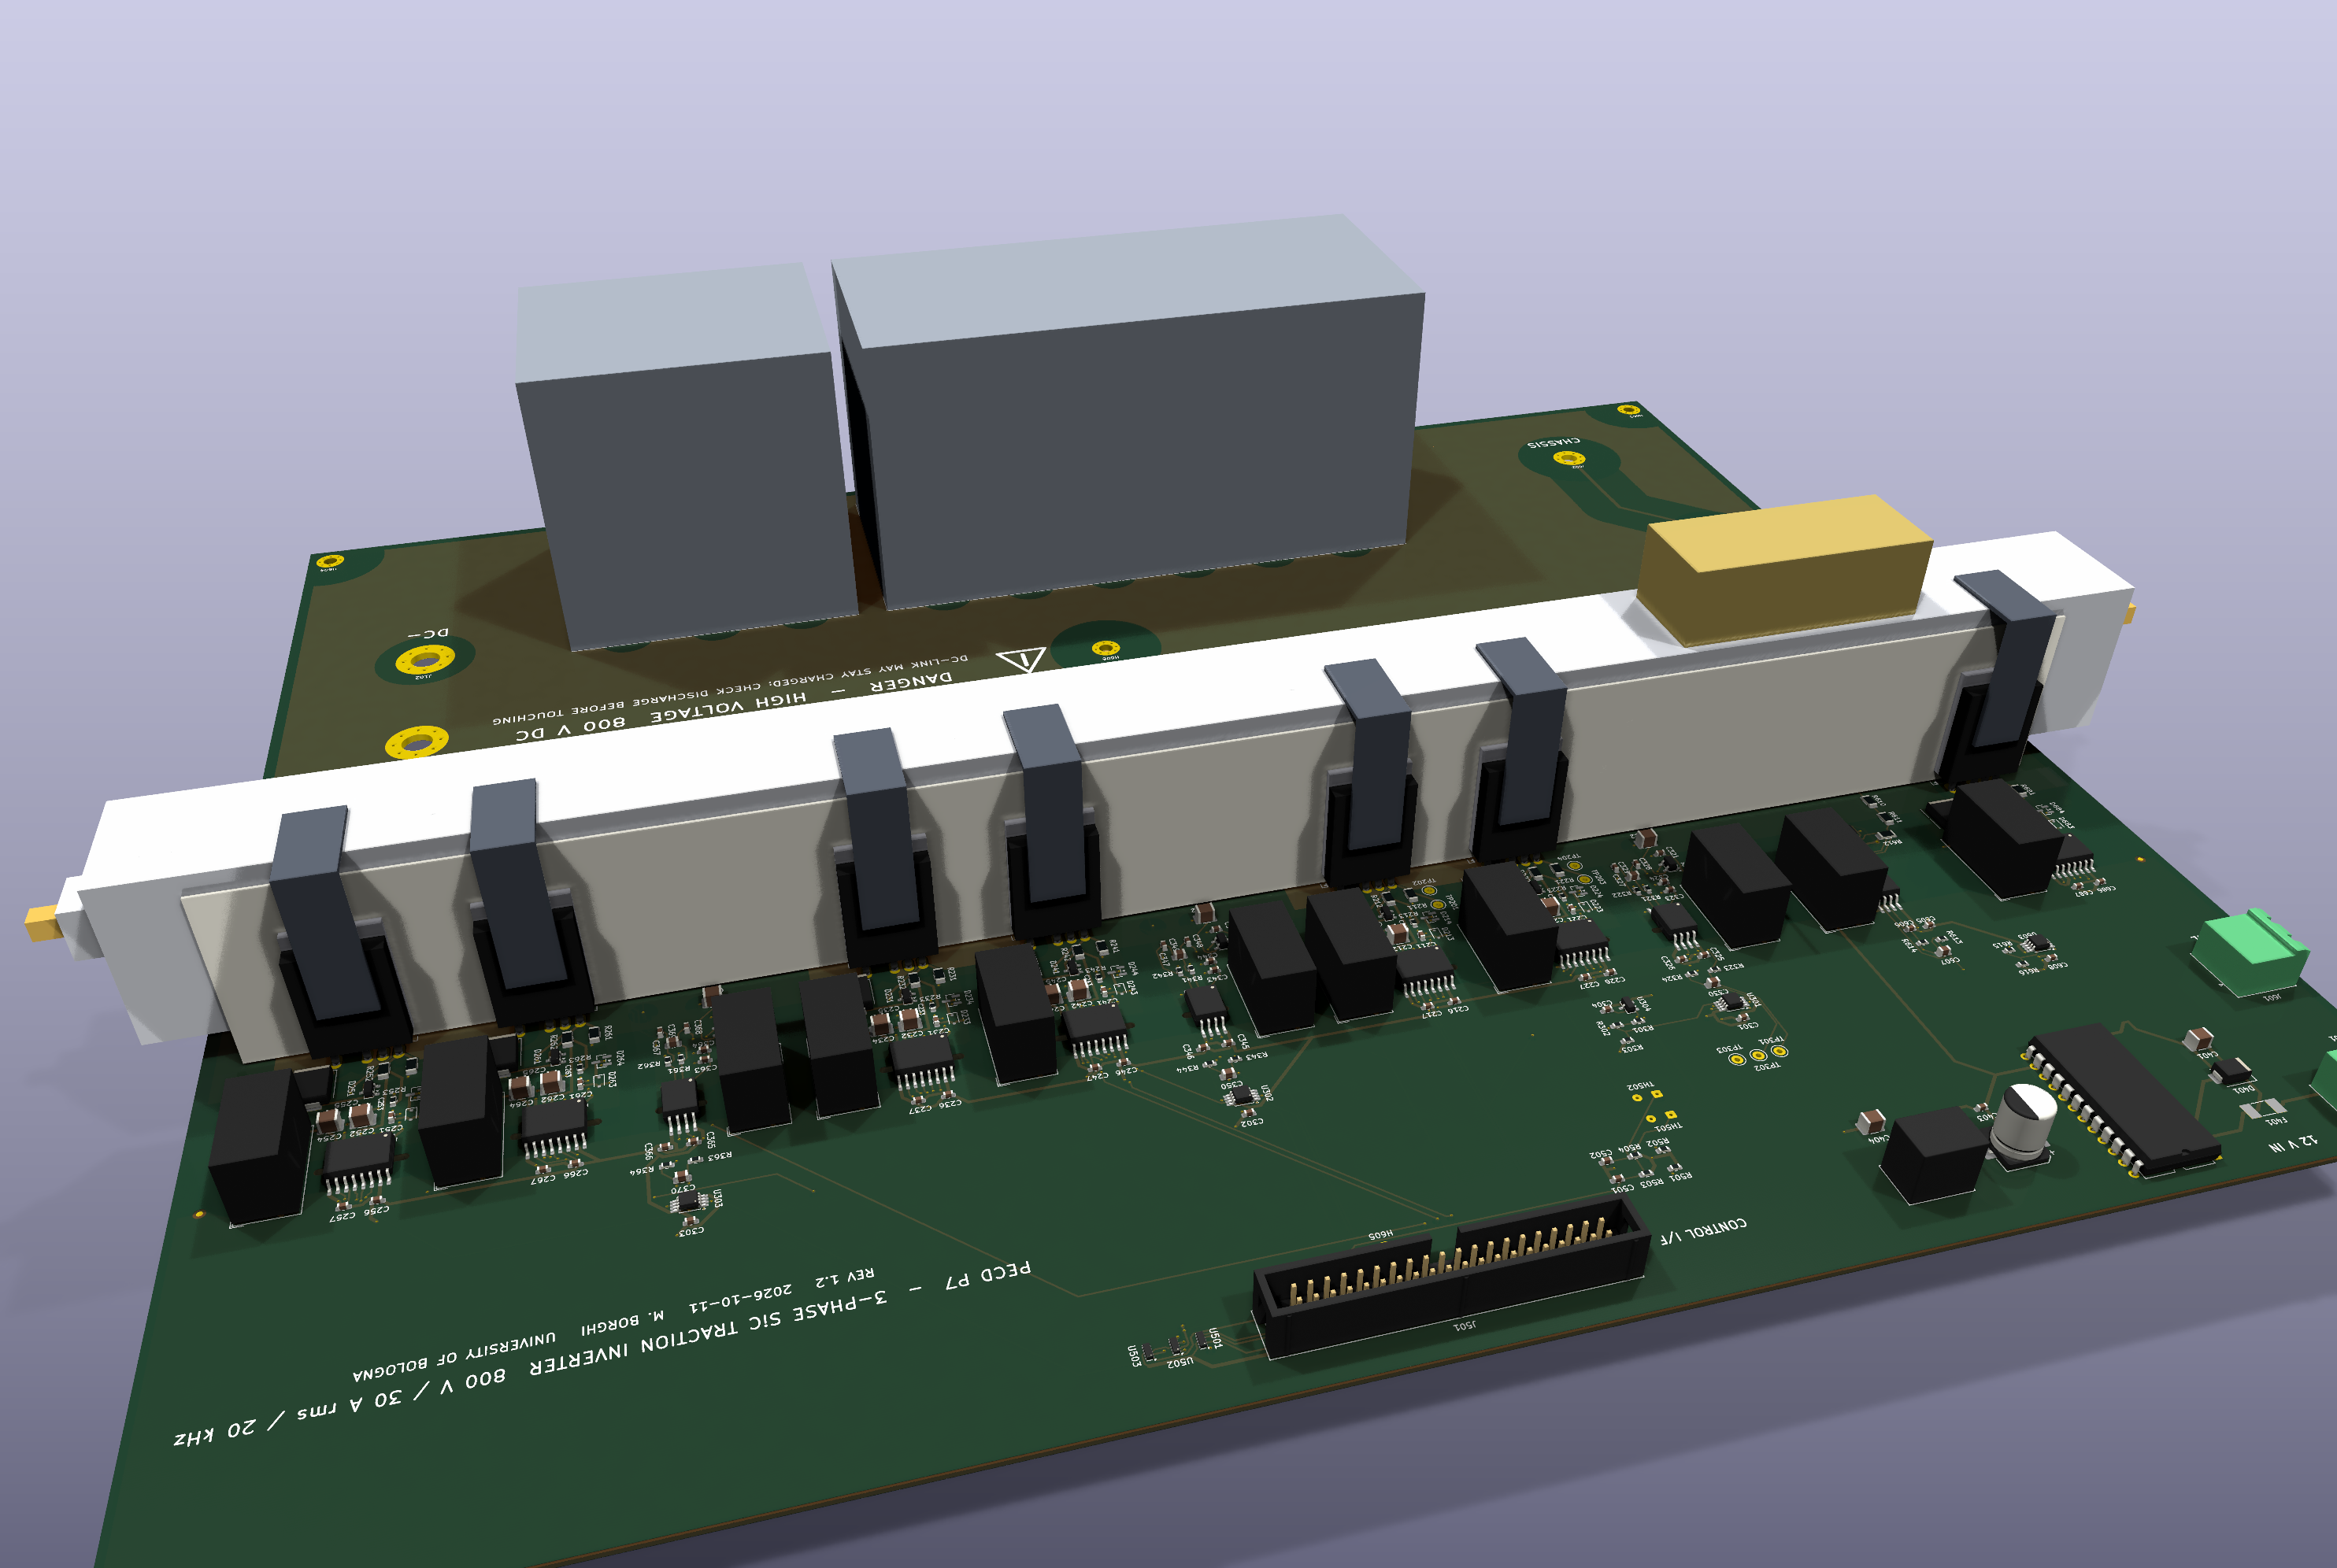
\includegraphics[width=\textwidth]{figures/kicad_meccanica_3d_nord.png}
  \caption{Cooling rail, insulating strip and spring clips on the frozen board,
  seen from the driver side (indicative bodies; the discharge resistor is
  the block on top of the rail).}
  \label{fig:mech3d}
\end{figure}

\paragraph{The profile is set by two distances.} The rail is chassis, so it
must keep \SI{5}{\milli\metre} of air from every high-voltage conductor;
and the creepage from tab to rail around the edge of the pad must reach the
\SI{9.0}{\milli\metre} of a reinforced barrier in pollution degree 2. The
pad cannot extend below the board, so the second condition is met by
raising the rail instead: its lip starts \SI{7.5}{\milli\metre} above the
board, and the path down the pad, under its edge and up to the rail is
\SI{10.1}{\milli\metre} (\cref{fig:mechsection}). The price is that the tab
touches the rail over \SI{81}{\percent} of its height; the uncovered strip
is the lowest \SI{4.5}{\milli\metre}, and the tab, two millimetres of
copper, spreads the heat into the contact area. The lip is
\SI{7}{\milli\metre} thick so that it passes beside the commutation
ceramics; the wide part with the channels starts \SI{13}{\milli\metre} up,
above everything on the board.

\begin{figure}[htbp]
  \centering
  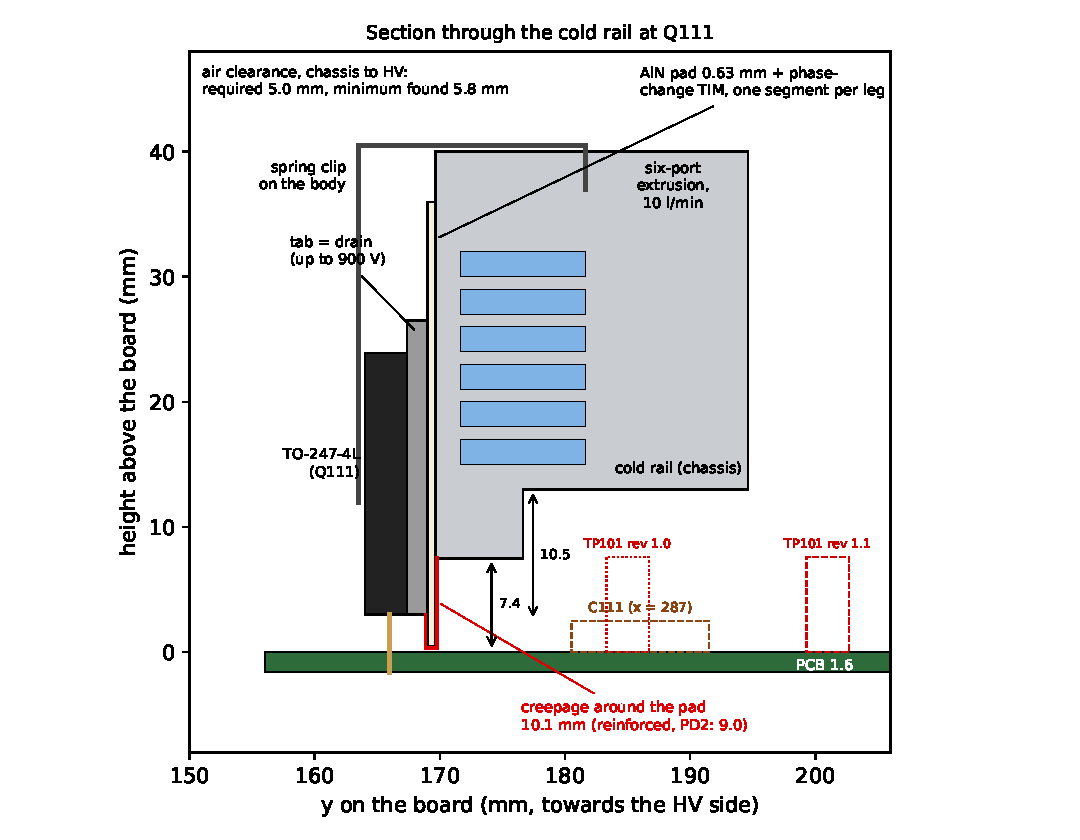
\includegraphics[width=0.92\textwidth]{figures/kicad_meccanica_sezione.pdf}
  \caption{Section through the rail at the high-side device of leg~1, with
  the creepage path around the pad and the two air clearances that set the
  profile. Dashed: parts behind the section plane.}
  \label{fig:mechsection}
\end{figure}

\paragraph{What the check found.} Every chassis part was checked in three
dimensions against every component and copper area of a high-voltage or
floating net, with component heights from their datasheets. The first
profile failed twice: the gate test points of leg~1, \SI{7.6}{\milli\metre}
tall, stood \SI{4.45}{\milli\metre} from the rail, and the commutation
ceramics passed with \SI{0.3}{\milli\metre} of margin. Revision 1.1 moves
the test points \SI{1.5}{\milli\metre} away and moves the switching-node test
point out from under the rail, where no probe could reach it; the profile
was thinned and raised. All parts now keep at least
\SI{5.8}{\milli\metre} of air. The rail, pad and clip outlines are drawn on
the board's documentation layer, so the assembler sees them.

\paragraph{Assembly order.} The devices are soldered \emph{after} they are
clamped to the rail. Soldered first, the leads would carry every tolerance
between the hole pattern and the rail, and the joints of a
\SI{20}{\milli\metre}-tall package would crack at the first thermal cycles.

\section{Design rules as implemented}
\label{sec:rules}

The distances of \cref{sec:insulation} are only as good as the check that
enforces them, and KiCad checks what its rules file says~\cite{kicad10}.
The file translates the coordination into constraints between net classes
(\cref{tab:netclasses}) and named areas, ordered so that every exception
comes after the rule it corrects; \cref{tab:rules} gives the ones that
carry the insulation concept.

\begin{table}[htbp]
\centering
\caption{Design rules that implement the insulation coordination.}
\label{tab:rules}
\small
\begin{tabularx}{\textwidth}{Ylr}
\toprule
Between & Insulation & Clearance \\
\midrule
two different high-voltage nets & functional & \SI{4.5}{\milli\metre} \\
\quad exception: drain and source inside the package area & functional & \SI{3.2}{\milli\metre} \\
\quad inner layers: negative plane to other HV nets and high-side domains (rev.~1.1) & functional & \SI{2.25}{\milli\metre} \\
\quad intermediate nodes of divider and bleeder & functional & \SI{1.6}{\milli\metre} \\
a floating domain and any high-voltage net other than its own reference & functional & \SI{4.5}{\milli\metre} \\
a floating domain and its own reference & --- & \SI{0.2}{\milli\metre} \\
two different floating domains & functional & \SI{4.5}{\milli\metre} \\
high voltage or a floating domain and the control side & reinforced & \SI{9.5}{\milli\metre} \\
\quad exception: the two pad rows of an isolator & reinforced, component & \SI{8.0}{\milli\metre} \\
\quad exception: the pins of an isolated supply (A.25) & functional & \SI{5.5}{\milli\metre} \\
a net that matches no class and anything hazardous & reinforced & \SI{9.5}{\milli\metre} \\
chassis, and the fixing holes, and anything hazardous & reinforced & \SI{9.5}{\milli\metre} \\
hazardous copper and the board edge & functional & \SI{2.25}{\milli\metre} \\
any copper under an isolator body & --- & forbidden \\
\bottomrule
\end{tabularx}
\end{table}

\paragraph{What changed while the board was laid out.} Five rules were
added or corrected once real copper existed, each found by the board rather
than by the analysis.
\begin{itemize}
  \item \emph{One class per domain} (\cref{ch:schematic}): a single class for
        all gate domains made the gate and the Kelvin source of the same
        device a violation.
  \item \emph{Unused pins.} KiCad gives every unused pin a net of its own;
        the rules first read those nets as unclassified, hence low voltage,
        and demanded \SI{9.5}{\milli\metre} between the pins of one package.
        They are now treated as having no net.
  \item \emph{Fixing holes.} The six M3 holes have no net, because the screw
        is earthed through the enclosure and not through the board; without a
        net they fell under the no-net rule, \SI{0.15}{\milli\metre}. A rule
        placed after it gives them the chassis distance back, and the copper
        of the positive rail stops \SI{10}{\milli\metre} from them.
  \item \emph{Width warnings.} The two signal-level connections on power nets
        are exempted by name and by area, as described under conductor
        sizing, so that a warning on those nets always means a real
        conductor.
  \item \emph{Inner layers} (revision 1.1). A surface creepage applied inside
        the laminate cost a third of the commutation loop
        (\cref{sec:loopextract}); the inner-layer value of IPC-2221B
        replaces it for the negative plane only.
\end{itemize}

\paragraph{The rules are themselves tested.} A rule with a syntax error is
silently ignored by the command-line checker, and a rule with a wrong
condition passes everything. A test board places the project's own
footprints on their real nets, once correctly and once in each wrong way,
and the check must report exactly the rule expected for each wrong case and
nothing for the correct ones; it is run after every change to the rules file.

\section{Verification and freeze}
\label{sec:freeze}

The board was first frozen on 11 October 2026 as revision 1.0, and the same
day again as revision 1.1, after the extraction and the mechanical
check had found what the design rule check could not: the phase-pour neck,
the cost of the clearance holes, and the test points too close to the rail.
Revision 1.1 changes copper and test-point positions only; the circuit is
the same. Each revision is recorded together with the exact files its
checks (\cref{tab:freeze}) were run on.

Revision 1.2 adds only what the fabricator and the assembler need:
three fiducials for automatic placement, a box for the serial number, a
drawing of the areas to mask before coating, and assembly notes (the
bleeders raised off the board, \cref{sec:complife}; the devices clamped to the
rail before they are soldered). No signal or power copper moves. Writing the
rule that keeps the fiducials, copper without a net, \SI{9.5}{\milli\metre}
from high voltage exposed a behaviour of the rule engine: a
clearance set locally on a pad (the library fiducial carries one) overrides
the custom rules, so the new rule stayed silent until the test board was made
to violate it. The local value was removed and the test board now carries the
case.

\begin{table}[htbp]
\centering
\caption{Checks passed by the frozen board.}
\label{tab:freeze}
\small
\begin{tabularx}{\textwidth}{lY}
\toprule
Check & Result \\
\midrule
Design rule check, all severities, zones refilled & 0 violations, 0 unconnected items \\
Board against schematic & 0 differences \\
Schematic against the independent model & 275 of 275 parts, pin by pin \\
ERC & one warning, intended (\cref{ch:schematic}) \\
Rules test board & every case as expected, 19 track cases among them \\
Routing checks, project script & 8 of 8: no track on the ground planes or inside the negative plane;
  no track on the wrong side of the barrier; class widths; gate loop
  $\leq\SI{25}{\milli\metre}$ in every channel; sensing pairs coupled \\
Geometry & 2168 segments, all at \SI{0}{}, \SI{45}{} or \SI{90}{\degree} \\
Commutation loop, extracted & \SI{7.8}{\nano\henry} of copper per leg, about
  \SI{8.3}{\nano\henry} with ESL, against the \SI{20}{\nano\henry} limit (\cref{sec:loopextract}) \\
Gate loop, extracted & \SI{13}{\nano\henry} of copper; die peak \SI{1040}{\volt} in the double pulse \\
Mechanics & every chassis part $\geq\SI{5.8}{\milli\metre}$ of air from HV; creepage around
  the pad \SI{10.1}{\milli\metre} (\cref{sec:mechanics}) \\
Silkscreen & every reference visible, upright, \SI{1.0}{\milli\metre} high
  (\SI{0.8}{\milli\metre} where crowded), stroke \SI{0.15}{\milli\metre},
  off the pads and nearer to its own part than to any other \\
Board markings & name, revision, HV warning with a warning triangle,
  terminal and connector labels \\
Fabrication outputs & Gerber, drill, placement, bill of materials,
  assembly drawing: generated by script, after a blocking rule check \\
\bottomrule
\end{tabularx}
\end{table}

What the freeze does \emph{not} settle is listed where it belongs: the
\emph{measured} loop inductance, which the extraction predicts but does not
replace (A.14), and the reinforced rating of the isolated supplies (A.25).

\subsection{Planned for later revisions}
\label{sec:nextrev}

The frozen board is the exam design. What a production version would change
is listed here, in the order it would be done.

\begin{itemize}
  \item Reinforced auxiliary supplies and a discharge that survives
        the loss of \SI{12}{\volt} (A.25, A.L1): a revision of the auxiliary
        supply, with new modules and footprints.
  \item Automotive-qualified replacements for the parts that are not:
        isolated converters, the \SI{12}{\volt} pre-regulator, connectors,
        the transient suppressor, the fuse.
  \item Four layers instead of six (\cref{sec:stackup}): the negative
        DC plane and the ground planes share one inner layer, the
        \SI{1.2}{\metre} of control tracks on L2 move to the remaining signal
        layer. The commutation loop does not change, since the plane stays
        \SI{0.10}{\milli\metre} under L1. Estimated saving about \SI{120}{}~EUR
        per board on a prototype run and \SI{40}{}~EUR in series of a hundred,
        the whole of it in the bare board; best done together with moving the
        film capacitors onto a laminated busbar off the board.
  \item Internally isolated TO-247-4 power devices once one is
        offered at this resistance with automotive qualification
        (\cref{sec:coolalt}): same footprint, no external pad.
  \item The input EMI filter of \cref{tab:emcfilter}, outside the
        board between battery and DC terminals: two \SI{0.62}{\milli\henry}
        common-mode chokes in series, whose leakage serves the differential
        mode, and a \SI{1}{\micro\farad} X-capacitor. The board does not
        change for it; the measurement confirms it once the limit class is
        fixed (A.19).
  \item The bill of materials of \cref{app:bom}, redone on the
        production revision.
\end{itemize}

\chapter{Conclusions}
\label{ch:conclusions}

The power stage of a three-phase two-level SiC inverter for \SI{800}{\volt},
\SI{30}{\Arms} and \SI{20}{\kilo\hertz} has been designed, with its cooling
and the schematic and layout of the module. This chapter sets the results
against the brief, names what remains open, and says where the design would
go next.

\section{Results against the brief}

\begin{table}[htbp]
\centering
\caption{The design against the brief and against the device criteria of
\cref{tab:criteria}.}
\label{tab:results}
\small
\begin{tabularx}{\textwidth}{L{0.26\textwidth}YL{0.2\textwidth}}
\toprule
Asked & Achieved & Where \\
\midrule
\SI{800}{\volt}, \SI{30}{\Arms} at any power factor &
  \SI{25.48}{\kilo\watt}, \SI{128.1}{\watt} of loss, efficiency \SI{99.50}{\percent} at the rated point;
  \SIrange{127.5}{128.1}{\watt} for $\cos\varphi \leq 0.87$ and \SI{131.5}{\watt} at unity & \cref{ch:losses}, \cref{sec:pfsweep} \\
\SI{20}{\kilo\hertz} &
  \SIrange{90.5}{166.1}{\watt} and $\Tj$ \SIrange{76.9}{86.8}{\celsius} over \SIrange{10}{30}{\kilo\hertz} &
  \cref{ch:losses} \\
Negligible output current ripple &
  \SI{2.46}{\ampere} peak-to-peak, \SI{0.84}{\percent} in RMS terms, with \SI{2.5}{\milli\henry} of load &
  \cref{ch:modulation} \\
DC-link voltage ripple $< \SI{0.5}{\percent}$, worst case &
  \SI{0.17}{\percent} at the rated point; \SI{2.86}{\volt}, \SI{0.36}{\percent}, in the worst case with \SI{200}{\micro\farad} &
  \cref{sec:dclink}, \cref{ch:model} \\
Forced air or liquid, \SI{50}{\celsius} ambient &
  liquid, six-port rail and AlN pad: \SI{77.1}{\celsius} at the rated point, \SI{97.9}{\celsius} at locked rotor, \SI{117.8}{\celsius} with all tolerances, against \SI{150}{\celsius};
  one fan with the same pad: \SI{108.3}{} and \SI{129.1}{\celsius} &
  \cref{sec:cooling} \\
\midrule
C1, locked rotor $\leq \SI{120}{\celsius}$ & \SI{97.9}{\celsius} & \cref{sec:coolalt} \\
C2, die $\leq \SI{1080}{\volt}$ at \SI{950}{\volt}, \SI{60}{\ampere} &
  \SI{1073.5}{\volt} at the \SI{20}{\nano\henry} budget; \SI{1040}{\volt} with the loop extracted from the copper &
  \cref{sec:kelvin}, \cref{sec:loopextract} \\
C3, drain--source creepage at \SI{900}{\volt} &
  \SI{3.24}{\milli\metre} against \SI{2.80}{\milli\metre} in PD1, with conformal coating &
  \cref{sec:insulation} \\
C4, automotive & power device AEC-Q101 qualified & \cref{sec:deviceselection} \\
C5, declared $t_\mathrm{SC} \geq \SI{1.5}{\micro\second}$ & \textbf{open}: not declared by the manufacturer & \cref{app:assumptions}, A.3 \\
\bottomrule
\end{tabularx}
\end{table}

The brief is met wherever the design can show it, with one open point: the
short-circuit withstand time, which the manufacturer does not declare and
which no simulation can replace. The stalled motor, a requirement this
design added, sizes the design. It decided the device and the pad, and it is
met with \SI{22}{\celsius} of margin on the criterion once the heat path is
designed rather than assumed.

\section{What remains open}

Three assumptions carry the thermal and the switching results, and each is
listed in \cref{app:assumptions} with the way to close it. The case-to-sink
resistance of the mounted pad (A.5) is the largest single uncertainty. The
loop inductance (A.7) is extracted from the copper, not measured, and the
gate resistance was chosen at \SI{20}{\nano\henry}, \SI{12}{\nano\henry}
above the extracted value. The switching energies (A.4) come from the
datasheet because the model underestimates them by a factor of 3.4 at turn-on.

\section{Possible developments}

\paragraph{Discontinuous modulation at standstill.} Clamping the phase that
carries the peak current to the positive rail lowers the hottest junction at
locked rotor by about \SI{12}{\celsius} on the real rail with the adopted pad
and the converter loss by a third (\cref{sec:lrdpwm}). It stays a
recommendation to the controller (\cref{tab:sysassume}), because hardware is
not sized on a control strategy the module cannot guarantee.

\paragraph{Internally isolated packages.} A TO-247-4 with the ceramic inside,
under the die, removes the external pad and one interface with the same
footprint (\cref{sec:coolalt}). When one is offered at this resistance with
automotive qualification it is the natural next step for the power devices.

\paragraph{A power module.} The discrete TO-247-4L sets two ceilings. The
first is inductance: \SI{14.6}{\nano\henry} of package contribution that no
layout can remove (\cref{sec:kelvin}), which forces
$R_{g,\mathrm{off}}$ to \SI{12.5}{\ohm} and makes switching more than half
of the loss budget. The second is insulation: the \SI{5.08}{\milli\metre}
lead pitch leaves \SI{3.24}{\milli\metre} of creepage between drain and
source, which passes with \SI{16}{\percent} of margin only under conformal
coating, and which IEC 60664-4~\cite{iec606644} would derate above
\SI{30}{\kilo\hertz}, the upper end of the sweep of \cref{tab:sweep-fsw}. A
power module with an integrated busbar lifts both ceilings together. The
selection study of \cref{sec:deviceselection} found none that fits at
\SI{30}{\Arms}: the small six-packs are industrial and run hot, and the
automotive single-switch modules are meant to be sintered onto a cooler. At a
few times the current a module would be the only answer.


% ------------------------------------------------------------- bibliografia
\cleardoublepage
\phantomsection
\addcontentsline{toc}{chapter}{Bibliography}
\printbibliography[title={Bibliography}]

% ---------------------------------------------------------------- appendici
\appendix
\chapter{Open assumptions}
\label{app:assumptions}

This appendix collects the quantities that are assumed rather than measured
or read from a datasheet. They are gathered in one place because these are
the points at which the design would change if the assumption turned out to
be wrong.

They are ordered by how much they would change the result. Their numbers are
identifiers rather than positions: the chapters and the bench plan refer to
them, so they were kept when an item moved between sections.

\section{Would change the design}

\paragraph{A.1 Pollution degree 1, obtained by conformal coating.}
Every insulation distance in this design, functional and reinforced
alike, is qualified in pollution degree 1, which is claimed on the basis
that the high-voltage area is conformally coated on both faces. The
coating is an existence condition: in pollution degree 2
the functional requirement at the \SI{900}{\volt} working voltage is
\SI{9.00}{\milli\metre} on ordinary FR-4 where the \device{} package offers
\SI{3.24}{\milli\metre} between its drain and source pads, and no layout can
recover a factor of \num{2.8}. At \SI{900}{\volt} the coating also carries
the reinforced barrier under the isolator bodies (A.24). If the coating is refused, the board is not buildable with
this device, and the answer is a different package, not a different layout.

The assumption is a \emph{process} condition rather than a dimension. A design rule check verifies
dimensions and passes the board either way. This is why it is written at the
head of the rules file, on the fabrication drawing, and here. See
\cref{sec:insulation}.

It is no longer only an assumption of process. The coating is specified with
a UV tracer and every board is inspected under UV light over the whole
high-voltage area (\cref{sec:isoslot}), so each board carries the evidence
that the condition holds on it. What remains assumed is the coating's
long-term integrity, not its presence.

\paragraph{A.2 Rated impulse withstand voltage, and the non-applicability of
overvoltage category.}
Clearance follows from an assumed rated impulse voltage, and because creepage
may not be smaller than clearance, that assumption can also set the creepage.
\SI{2.5}{\kilo\volt} is declared, derived from the transient the converter
generates internally (\SI{1148}{\volt} at the die in the worst simulated
case) rather
than from an overvoltage category, on the grounds that a battery-fed floating
system is not supplied from a low-voltage distribution network and cannot
receive a mains-borne impulse (\cref{sec:ovc}).

This is the critical entry of this group. The design passes at \SI{4}{\kilo\volt} with
\SI{8}{\percent} of margin and fails at \SI{6}{\kilo\volt}, which is what
overvoltage category II on a \SI{1000}{\volt} band would give. The argument
rests on three legs, and it falls if any one of them falls: the standard
provides for deriving the impulse from the actual transient where the circuit
is not mains-supplied; that transient is simulated rather than assumed; and
the declared level is \num{2.2} times the worst simulated peak.

\paragraph{A.3 Table values of IEC 60664-1, and their source.}
The creepage and clearance requirements used throughout
\cref{sec:insulation} come from a third-party calculator implementing a
stored subset of the standard~\cite{standardclarity}, not from the text of
IEC 60664-1~\cite{iec60664}, which was not available.

The calculator checked nine values that had been quoted from memory (five
creepage rows, two clearance rows, the reinforced doubling rule and the
pollution-degree floor), and all nine agreed to the digit. A published,
reproducible secondary source that confirms every value is a different kind
of evidence from a recollection. It is still not the standard: it covers a
stored subset and describes itself as a reference estimate, so the text is to
be read before release. A.2 weighs more than this entry.

\paragraph{A.4 Galvanic isolation in the charging path.}
The argument that overvoltage category does not apply (A.2) depends on the
high-voltage bus never being conductively tied to the mains. During charging
the contactors are closed and the bus \emph{is} connected to the inlet, so
what breaks the path is the galvanic isolation of the charging
equipment (the on-board charger's transformer in AC charging, the station's
in DC charging). Both sit outside this perimeter, and the assumption is
recorded as requirement R10 (\cref{tab:sysreq}).

It is not normatively guaranteed. IEC 61851-23~\cite{iec6185123}
distinguishes isolated from non-isolated DC charging stations, imposing
additional protective measures on the latter, so a vehicle that accepts any
station cannot assume isolation. If the assumption fails, the insulation
coordination moves into a different normative domain rather than
losing margin, and the mitigation belongs at the charge inlet, not on this
board. This is the second most load-bearing assumption in the
design, after A.1.

\paragraph{A.5 Short-circuit withstand time, carried as a threshold.}
The \device{} datasheet does not declare $t_\mathrm{SC}$, the only
selection criterion the chosen device leaves undemonstrated. It is carried
as a threshold (\cref{sec:tsc}): counted as the manufacturer measures it,
the protection chain closes in \SI{0.69}{\micro\second} typical and
\SI{0.83}{\micro\second} worst case, so the design survives a short
if $t_\mathrm{SC} \geq \SI{0.83}{\micro\second}$ and has a factor of two at
\SI{1.66}{\micro\second}. A class value from the manufacturer, on a
\SI{16}{\milli\ohm} die of the same generation at \SI{+15}{\volt}, gives
\SI{2.4}{\micro\second} at \SI{950}{\volt} once scaled at constant
energy~\cite{wolfspeed_scan}: a factor of 2.9, but on another part. The
plan B is sized (\cref{sec:planb}): with a \SI{4.7}{\pico\farad} blanking
capacitor and a \SI{4.7}{\volt} zener the protection covers
\SI{0.71}{\micro\second}; below that, desaturation detection is the wrong
principle for this device. The value is to be obtained from the
manufacturer in writing or from test B1 of \cref{tab:benchplan}, before the
protection is trusted.

\paragraph{A.6 Switching energy: model against datasheet.}
At the datasheet test point the SPICE model gives $\Eon = \SI{748}{\micro\joule}$
against \SI{2552}{\micro\joule} measured, a factor of 3.4, and
$\Eoff = \SI{509}{}$ against \SI{788}{\micro\joule}, a factor of 1.55
(\cref{sec:kelvin}); the device of the first iterations showed the same
factor on turn-on. The loss budget uses the datasheet, on the grounds that it
is a measurement, but this is the first thing to verify on the
bench: if the model is right, the thermal budget improves considerably. The
overshoot results do not depend on it: they come from the same model's
waveforms, not from its energies.

\paragraph{A.7 Insulating pad thermal resistance.}
$\Rthcs = \SI{0.50}{\celsius\per\watt}$ is a class value, not a product
figure, and it also depends on the mounting torque. Across the plausible
range it moves the nominal junction temperature by \SI{23}{\celsius}
(\cref{tab:rthcs}) and never threatens the rated point. At locked rotor it
does: C1 holds only up to \SI{0.62}{\celsius\per\watt}, about
\SI{7}{\celsius} per tenth (\cref{sec:lockedrotor}). The pad value is
therefore a mounting specification, torque included, and not a free choice;
it is the largest single uncertainty in the numbers quoted and the first
thing to measure on a mounted sample. On the real rail (\cref{sec:cooling})
the limit tightens to \SI{0.50}{\celsius\per\watt}, and the design adopts
aluminium nitride with a phase-change interface material at
\SI{0.18}{\celsius\per\watt}; the interfaces decide the value more than the
ceramic does (\cref{sec:coolalt}).

\paragraph{A.8 Sampling rate and sampling instant.}
The analogue interface of \cref{sec:analogif} is designed for
$f_s = \fsw = \SI{20}{\kilo\hertz}$, one sample per switching period, taken
synchronously with the carrier peak or valley. This is standard practice in
machine control and it is what makes a current loop of a few kilohertz
sensible, but the controller has not been selected and the rate has not been
agreed with anyone.

Two things follow from it. The anti-aliasing corner is placed at
\SI{106}{\kilo\hertz} rather than near Nyquist \emph{because} synchronous
sampling already nulls the ripple; if the sampling turned out to be
asynchronous, the ripple would alias, the filter would have to move down by
a decade, and the \SI{16}{\micro\second} of delay that follows would not fit
the current loop, and the board would then need its own ADC, which reverses the
boundary decision of \cref{sec:sysreq}. And the reading error moves from zero
to $\pm\SI{4.10}{\percent}$ of rating (\cref{tab:sampling}).

It is therefore written as requirement R6 rather than left as an
assumption, because the board depends on something that happens outside
it. It is listed here because a requirement that the
system cannot meet is an assumption again.

\paragraph{A.22 Coolant temperature.}
The \SI{65}{\celsius} coolant is this design's assumption, not part of the
specification (\cref{tab:spec}). At \SI{70}{\celsius} the locked-rotor
junction temperature rises by about \SI{6}{\celsius}: on the ideal plate of
\cref{sec:lockedrotor} it stays within C1 with a few degrees to spare, on the
cooling rail adopted in \cref{sec:coolalt} it reaches \SI{117.8}{\celsius} only
with every other tolerance stacked on top (\cref{tab:coolalt}). It is a requirement on the vehicle's cooling loop and should be
written as one.

\paragraph{A.23 Maximum continuous battery voltage.}
Every working-voltage quantity (creepage, the static derating of the
devices, the voltage class of the film capacitor, the divider) is sized at
\SI{900}{\volt}. That is requirement R12 on the battery, including charging
and regenerative braking; a pack that sits above it for long enough to count
as ``continuous'' is outside this design.

\paragraph{A.25 The isolated DC/DC converters (open decision).}
The eleven converters that supply the drivers and the sensing cross the
HV-to-control barrier, and their datasheet recognises them as reinforced
insulation only up to \SI{150}{\volt} rms, basic up to \SI{300}{\volt} rms,
functional up to \SI{2.4}{\kilo\volt}~\cite{murata_mgj2}. At
\SI{900}{\volt} they are functional insulation. The reinforced
barrier declared in this report is therefore not met at these components.
Two ways out, both changing the design: supplies rated for reinforced
insulation at a working voltage of at least \SI{900}{\volt} DC, or a
safety barrier placed elsewhere in the system with the board's HV-to-control
insulation declared functional. It is the one open point of this appendix
that is a safety question rather than a margin question.

The schematic and the board were frozen with these converters, so
the frozen board implements the second option as far as the board can: the
rules file treats the converter pins as functional insulation, at
\SI{5.5}{\milli\metre}, and declares it by name (\cref{tab:rules}); every
other crossing of the barrier (isolators, board copper, the slots) is
reinforced. Choosing the first option means a different module and a
different footprint, that is a board revision, not an edit.

\section{Would change a component choice}

\paragraph{A.9 Negative gate bias (resolved).}
\SI{-5}{\volt} is used. The datasheet's \SI{-4}{\volt} is a typical
operating value, not a limit; the absolute maximum is
\SI{-8}{\volt}~\cite{wolfspeed_e3m0016}, leaving \SI{3}{\volt} of margin. The
standard isolated module delivers \SI{-5}{\volt} without an extra
regulator, and the extra volt goes straight into the margin against spurious
turn-on (\cref{tab:miller}). See \cref{sec:negbias}.

\paragraph{A.10 Isolation grade of the gate-drive supply.}
The \dcdc{} withstands \SI{2400}{\volt} continuously but its \emph{certified}
reinforced rating is only \SI{150}{\Vrms}~\cite{murata_mgj2}. Functional
isolation has been assumed, on the basis that the HV system floats with
respect to chassis and the low-voltage side is not touchable. If certified
reinforced isolation is required across that barrier, the module must change.

\paragraph{A.11 Vehicle \SI{12}{\volt} rail range.}
Assumed \SI{9}{}--\SI{16}{\volt} continuous with larger transients, typical
of ISO 16750-2~\cite{iso16750}, without access to the standard itself. The
pre-regulator must be sized on the real range.

\paragraph{A.12 Terminal dimensions and voltage class of the ceramic capacitors.}
The decoupling capacitor carries up to \SI{900}{\volt} between its own two
terminals, so its creepage is the body length less the two terminations. On
the typical dimensions used here a 1210 leaves \SI{2.00}{\milli\metre}, below
the \SI{2.80}{\milli\metre} required, while a 1812 leaves
\SI{3.20}{\milli\metre}. The voltage class is \SI{1250}{\volt} or more, in
C0G: a \SI{1000}{\volt} part would work at \SI{90}{\percent} of its rating
at \SI{900}{\volt}, and an X7R one would lose most of its capacitance to the
bias. Resolved at capture (D8, \cref{tab:captdecisions}): a
\SI{220}{\nano\farad} part of that class does not exist; the largest C0G
ceramic at \SI{1200}{\volt} is \SI{47}{\nano\farad} in a 3640, whose
\SI{6.25}{\milli\metre} between pads passes with margin. Four are
fitted per leg, \SI{188}{\nano\farad}, at \SI{75}{\percent} of the rating at
\SI{900}{\volt}~\cite{kemet_kclink}.

\paragraph{A.13 Material group of the ceramic pad.}
The pad is sized in pollution degree 2 with the ceramic assigned material
group I, which requires a datasheet stating CTI $\geq \SI{600}{\volt}$.
Technical ceramics (aluminium nitride, adopted in \cref{sec:coolalt}, and
alumina) do not track, so the assignment is expected to hold, but it has not
been confirmed on a specific part. Material group II would take a pad
standing on its own from \SI{33}{}$\times$\SI{37}{} to
\SI{41}{}$\times$\SI{45}{\milli\metre} (\cref{tab:pad}); on the cooling rail,
where the creepage below the tab comes from raising the rail, it would mean
raising it further and checking the section of \cref{fig:mechsection} again.

The pollution degree at the pad is not in this appendix. Degree 1 at the pad
would rest on a sealed housing, a system-level property this design does not
own. Sizing the pad for
degree 2 removed the assumption at a cost of \SI{57}{\percent} more pad
area, the only point in this design where an assumption was eliminated
rather than declared.

\section{Would change the layout or the verification}

\paragraph{A.14 Loop inductance of the real layout.}
The \SI{20}{\nano\henry} limit is not yet a verified result, and it is now
load-bearing: $R_{g,\mathrm{off}} = \SI{12.5}{\ohm}$ keeps the die below
\SI{1080}{\volt} \emph{at} \SI{20}{\nano\henry}, with six and a half volts to spare.
In inductance that margin is \SI{2.6}{\nano\henry}: C2 fails at
\SI{22.6}{\nano\henry} at turn-off and at \SI{23.6}{\nano\henry} on
recovery (\cref{tab:lthreshold}), each known to about
$\pm\SI{1}{\nano\henry}$. Extracted on the frozen board
(\cref{sec:loopextract}), it is \SI{7.8}{\nano\henry} of copper in revision 1.1,
about \SI{8.3}{\nano\henry} with the capacitor ESL, so the verification
holds with \SI{14}{\nano\henry} to the threshold, and the double pulse with
the extracted values puts the die at \SI{1040}{\volt}. What remains assumed is
the extraction itself (a quasi-static model of the copper layers, with the
packages taken from the vendor's model) until test B2 measures it,
against the failure threshold rather than the limit, and
remembering that the figure to compare is the PCB contribution and not the
whole loop. Between \SI{20}{} and \SI{22.6}{\nano\henry} the design holds
as it is; above \SI{23}{\nano\henry} both gate resistors, the losses and the
thermal result of \cref{sec:lockedrotor} have to be recomputed.

\paragraph{A.15 IPC-2152 chart values.}
The conductor widths use the IPC-2221B closed form, which is conservative in
this configuration. The IPC-2152 charts were not available and their values
have not been invented. The layout was frozen without them; the one place
where the pours were narrower than the closed form asks, a neck below each
shunt pad, has a second pour on L6 since revision 1.1
(\cref{sec:conductors}), so the charts are expected to confirm rather than
change the result.

\paragraph{A.16 Copper temperature rise.}
A \SI{30}{\celsius} rise was assumed for conductor sizing
(\cref{tab:widths}). On a board already at \SI{67}{}--\SI{85}{\celsius} this
puts the copper near \SI{115}{\celsius}, which should be revisited against the
mechanical thermal design. The margin here is thinner than it was: the DC bus
current is \SI{32.0}{\ampere} rather than the \SI{22.5}{\ampere} first
assumed, so the bus conductor has to be \SI{60}{\percent} wider.

\paragraph{A.17 Dielectric strength of the prepreg, and the L1--L2 field.}
The \SI{0.10}{\milli\metre} prepreg chosen to minimise the plane-pair
inductance carries the full DC-link voltage, a field of
\SI{9}{\kilo\volt\per\milli\metre} at \SI{900}{\volt} against a laminate strength assumed to be
\SI{30}{}--\SI{40}{\kilo\volt\per\milli\metre}. This is functional
insulation, so the standard imposes no minimum thickness, but it is the
thinnest margin in the design and it cannot be inspected once the board is
pressed. A layer-to-layer withstand test at \SI{2}{\kilo\volt} DC for one
minute is specified on the fabrication drawing, which converts the assumption
into a measurement. Doubling the prepreg would halve the field and
cost \SI{0.19}{\nano\henry} (\cref{tab:planepair}), a trade to revisit at the
first prototype.

\paragraph{A.18 Y-capacitance permitted by the vehicle.}
The board carries \num{2}$\times$\SI{4.7}{\nano\farad}, not the
\num{2}$\times$\SI{22}{\nano\farad} first assumed: \SI{4.7}{\nano\farad} is
the largest Y1 disc rated \SI{1500}{\volt} DC (D12,
\cref{tab:captdecisions}). The function (closing the common-mode current to
chassis at high frequency) stays; its effectiveness is a matter for the
emission test, and the value must still be reconciled with the vehicle's
insulation-monitoring budget, which is a system-level constraint and not a
board-level one.

\paragraph{A.19 CISPR 25 edition and limit class.}
The estimate of \cref{sec:emcest} shows that an input filter is needed
whatever the class; the class decides its margin. It was taken against the
class~3 voltage-method limits of the low-voltage network as a reference,
since the limits that apply to the high-voltage lines and the class the
vehicle maker asks for are not fixed.

\paragraph{A.24 The reinforced barrier under the isolator bodies (decided: slot).}
A through slot is made under each of the seven drivers and four isolated
amplifiers (\cref{tab:slotdims}), and the driver footprint is changed to the
manufacturer's high-voltage land pattern, because the standard one left
\SI{7.25}{\milli\metre} and not the \SI{8}{\milli\metre} assumed until then.
The board path around each slot is at least \SI{9.8}{\milli\metre} against the
\SI{9.5}{\milli\metre} rule. What stays assumed is the package
surface: \SI{8.0}{} and \SI{8.5}{\milli\metre} against \SI{9.0}{\milli\metre}
in pollution degree 2, covered by the components' own reinforced rating and,
in the design basis, by the coating. The slot moves the barrier's weak point
from the uninspectable gap under the body to package faces that are coated
and inspected (\cref{sec:isoslot}).

\section{Accepted limitations}

These are known limits of the design as scoped, collected here so that
nobody has to discover them by reading every chapter.

\paragraph{A.L1 The active discharge depends on the auxiliary supply.}
The seventh gate-drive channel that switches the discharge resistor is fed
from the vehicle's \SI{12}{\volt} rail. If a crash interrupts that rail the
active discharge does not run and only the passive bleeder remains, which
takes \SI{121}{\second} to reach \SI{60}{\volt} from \SI{900}{\volt} against a
\SI{5}{\second} requirement~\cite{unr100}. This is the standard
architecture, in which the bleeder is a backstop and not a substitute, but
the gap is
recorded because it is a requirement unmet in that condition. A production
design would take the discharge control power from the HV bus itself.
See \cref{sec:dclinkmgmt}.

\paragraph{A.L2 Contactors, precharge and interlock monitoring are out of
scope.} The board receives an already-charged bus and carries the interlock
loop through without monitoring it. Its contribution is the DC-link voltage
measurement on which the vehicle controller closes the main contactor at
voltage rather than on a timer. The precharge sizing is given in
\cref{sec:scope} as a system-level result, not as a board function.

\section{Would change only the transient}

\paragraph{A.20 Cold-plate heat capacity and thermal resistance.}
$C_\mathrm{hs} = \SI{1000}{\joule\per\kelvin}$ is estimated from an assumed
plate geometry; it affects no steady-state temperature (verified by
re-running the complete sweep), but it sets the time constant, and therefore
how long a bench measurement must run before the reading is meaningful.
$\Rthha = \SI{0.01}{\celsius\per\watt}$ is no longer an assumption of the
design: it was the optimistic end of what cold plates achieve, and
\cref{sec:cooling} replaces it with the rail as drawn, computed in three
dimensions (equivalent to \SI{0.069}{\celsius\per\watt}). What remains
assumed there is the channel correlation, whose $\pm\SI{20}{\percent}$ moves
the hottest junction by \SI{0.8}{\celsius}, and a uniform flux under the
tab.

\section{Would change the safe state}

\paragraph{A.21 Load type.}
The entire report assumes a passive $RL$ bench load. With a permanent-magnet
machine the safe state would have to be re-examined: the back-EMF can feed the
DC-link with all devices off, and the usual answer is an active short circuit,
which is the opposite of turning everything off.

\section*{Bench verification plan}
\addcontentsline{toc}{section}{Bench verification plan}

The thresholds of this appendix are useful only if each is attached to a
measurement with a pass mark written before the measurement is made.

\begin{table}[htbp]
\centering
\caption{Bench verification plan: tests, pass marks and the assumption each closes.}
\label{tab:benchplan}
\small
\begin{tabularx}{\textwidth}{lYYl}
\toprule
 & Test & Pass mark & Closes \\
\midrule
B1 & Short circuit on a sacrificial device, hard fault at turn-on, \SI{950}{\volt}, \SI{175}{\celsius}, \SI{+15}{\volt}
   & survives $\geq\SI{0.83}{\micro\second}$; design margin at $\geq\SI{1.66}{\micro\second}$ & A.5 \\
B2 & Parasitic extraction of the power loop, PCB contribution only
   & $\leq\SI{20}{\nano\henry}$ target; C2 lost at \SI{22.6}{\nano\henry} & A.14 \\
B3 & Double pulse on the real board, \SI{950}{\volt}, \SI{60}{\ampere}, hot plate
   & pin voltage $\leq\SI{1055}{\volt}$ (die $\leq\SI{1080}{\volt}$) & A.14 \\
B4 & Switching energies at the datasheet point
   & between the model and the datasheet (\cref{sec:kelvin}) & A.6 \\
B5 & Case-to-plate resistance of the mounted pad, specified torque
   & $\Rthcs \leq \SI{0.18}{\celsius\per\watt}$ design value, \SI{0.50}{\celsius\per\watt} at most (\cref{sec:coolalt}) & A.7 \\
B6 & Locked rotor, \SI{42.4}{\ampere} DC, coolant \SI{65}{\celsius}, case thermocouple on the hottest device
   & $\Tcase \leq \SI{106}{\celsius}$, i.e.\ $\Tj \leq \SI{120}{\celsius}$ at typical $\Rthjc$; model \SI{84.5}{\celsius} on the six-port rail with the aluminium nitride pad (\cref{tab:coolalt}) & C1 \\
B7 & UV inspection of the coating, every board & complete coverage of the HV area & A.1 \\
\bottomrule
\end{tabularx}
\end{table}

% Generato da 02 - KiCAD/costi/appendice_bom.py: non modificare a mano.
\chapter{Bill of materials and cost}
\label{app:bom}

This appendix lists every part of the frozen board, revision 1.2, grouped by
schematic sheet, the parts outside the schematic that complete the inverter,
and what the whole costs. Prices are per part for a prototype run of five
boards and for a series of a hundred, in euro; where a distributor price was
found it is used, otherwise the value is an estimate of the same class, and the
source of each figure is recorded with the cost estimate.
The totals are an order of magnitude, $\pm\SI{30}{\percent}$, not a quotation:
an order needs quotes, and the production revision of \cref{sec:nextrev} will
replace a fifth of the parts.

\footnotesize
\setlength{\tabcolsep}{4pt}
\begin{longtable}{L{0.19\textwidth}L{0.16\textwidth}L{0.28\textwidth}rrr}
\caption{Bill of materials of revision 1.2, by schematic sheet. Unit prices for one
piece and for a hundred; the total is for one board at prototype prices.}
\label{tab:bom}\\
\toprule
References & Value & Order code, manufacturer & Qty & EUR (1/100) & Total \\
\midrule
\endfirsthead
\toprule
References & Value & Order code, manufacturer & Qty & EUR (1/100) & Total \\
\midrule
\endhead
\multicolumn{5}{l}{\textbf{Power stage}} & \textbf{491.00} \\
C101 & 140uF 1100V & MKP1848714914Y5, Vishay & 1 & 95.00 / 70.00 & 95.00 \\
C102 & 60uF 1100V & MKP1848660914Y5, Vishay & 1 & 45.00 / 32.00 & 45.00 \\
C111-C114, C121-C124, C131-C134 & 47nF 1200V C0G & CKC33C473KEGACAUTO, KEMET & 12 & 8.20 / 5.30 & 98.40 \\
Q111, \dots, Q132 & E3M0016120K & E3M0016120K, Wolfspeed & 6 & 40.00 / 30.00 & 240.00 \\
R111, R121, R131 & CSS2H-3920R-L500FE & CSS2H-3920R-L500FE, Bourns & 3 & 3.00 / 2.00 & 9.00 \\
TP101, \dots, TP302 & TP red & 5000, Keystone & 5 & 0.40 / 0.25 & 2.00 \\
TP102, TP202, TP204, TP303 & TP black & 5001, Keystone & 4 & 0.40 / 0.25 & 1.60 \\
\addlinespace
\multicolumn{5}{l}{\textbf{Gate drive (seven channels)}} & \textbf{204.28} \\
C211, \dots, C681 & 10pF C0G & GCM1885C1H100JA16D, Murata & 7 & 0.12 / 0.03 & 0.84 \\
C212, \dots, C684 & 10uF 50V X7R & GRM32ER71H106KA12L, Murata & 20 & 0.60 / 0.25 & 12.00 \\
C213, \dots, C687 & 100nF 50V X7R & GCM188R71H104KA57D, Murata & 40 & 0.12 / 0.03 & 4.80 \\
C216, \dots, C686 & 1uF 16V X7R & GCM188R71C105KA64D, Murata & 15 & 0.12 / 0.03 & 1.80 \\
D211, \dots, D681 & BZX84-C4V3 & BZX84-C4V3,215, Nexperia & 7 & 0.10 / 0.03 & 0.70 \\
D212, \dots, D682 & GP3D010A120S & GP3D010A120S, SemiQ & 7 & 5.26 / 3.22 & 36.84 \\
D213, \dots, D683 & BAT54J & BAT54J,115, Nexperia & 7 & 0.15 / 0.05 & 1.05 \\
D214, \dots, D684 & BZX84-C13 & BZX84-C13,215, Nexperia & 7 & 0.10 / 0.03 & 0.70 \\
PS211, \dots, PS681 & MGJ2D121505SC & MGJ2D121505SC, Murata Power Solutions & 11 & 9.00 / 6.07 & 99.00 \\
R211, \dots, R681 & 4.99 & CRCW12064R99FKEAHP, Vishay & 7 & 0.30 / 0.15 & 2.10 \\
R212, \dots, R682 & 12.4 & ERJ-P08F12R4V, Panasonic & 7 & 0.25 / 0.10 & 1.75 \\
R213, \dots, R683 & 1k & ERJ-3EKF1001V, Panasonic & 7 & 0.10 / 0.01 & 0.70 \\
U211, \dots, U681 & UCC21750-Q1 & UCC21750QDWRQ1, Texas Instruments & 7 & 6.00 / 4.50 & 42.00 \\
\addlinespace
\multicolumn{5}{l}{\textbf{Phase current sensing}} & \textbf{37.67} \\
C327, C347, C367 & 22nF C0G & GCM21B5C1H223JA16L, Murata & 3 & 0.40 / 0.15 & 1.20 \\
C328, \dots, C369 & 100pF C0G & GCM1885C1H101JA16D, Murata & 6 & 0.12 / 0.03 & 0.72 \\
C330, C350, C370, C607 & 15nF C0G & GCM2195C1H153JA16D, Murata & 4 & 0.35 / 0.12 & 1.40 \\
R301 & 1.21k & ERJ-3EKF1211V, Panasonic & 1 & 0.10 / 0.01 & 0.10 \\
R302 & 2.15k & ERJ-3EKF2151V, Panasonic & 1 & 0.10 / 0.01 & 0.10 \\
R303, R501, R502, R616 & 10k & ERJ-3EKF1002V, Panasonic & 4 & 0.10 / 0.01 & 0.40 \\
R321, \dots, R362 & 2.2 & ERJ-3RQF2R2V, Panasonic & 6 & 0.10 / 0.01 & 0.60 \\
R323, \dots, R614 & 49.9 & ERJ-3EKF49R9V, Panasonic & 8 & 0.10 / 0.01 & 0.80 \\
U301-U303, U603 & TLV1702-Q1 & TLV1702AQDGKRQ1, Texas Instruments & 4 & 1.50 / 0.90 & 6.00 \\
U304 & LM4040-2.5 & LM4040QBIM3-2.5/NOPB, Texas Instruments & 1 & 1.00 / 0.60 & 1.00 \\
U321, U341, U361 & AMC1302-Q1 & AMC1302QDWVRQ1, Texas Instruments & 3 & 6.72 / 5.00 & 20.15 \\
U322, U342, U362, U602 & TPS7B6950-Q1 & TPS7B6950QDBVRQ1, Texas Instruments & 4 & 1.30 / 0.80 & 5.20 \\
\addlinespace
\multicolumn{5}{l}{\textbf{Auxiliary supply}} & \textbf{36.02} \\
C402 & 220uF 25V & EEE-FK1E221P, Panasonic & 1 & 0.60 / 0.30 & 0.60 \\
C403 & 1uF 25V X7R & GCM188R71E105KA64D, Murata & 1 & 0.12 / 0.03 & 0.12 \\
D401 & SMBJ18A & SMBJ18A, Littelfuse & 1 & 0.30 / 0.12 & 0.30 \\
F401 & 2A T & 0452002.MRL, Littelfuse & 1 & 1.30 / 0.80 & 1.30 \\
PS401 & TEN 8-1212 & TEN 8-1212, TRACO Power & 1 & 30.20 / 26.00 & 30.20 \\
PS402 & R-78E3.3-0.5 & R-78E3.3-0.5, RECOM & 1 & 3.50 / 2.60 & 3.50 \\
\addlinespace
\multicolumn{5}{l}{\textbf{Control interface}} & \textbf{9.73} \\
J501 & WR-BHD 2x20 & 61204021621, Wurth Elektronik & 1 & 1.60 / 1.10 & 1.60 \\
J502 & MSTBA 2,5/2-G-5,08 & 1757242, Phoenix Contact & 1 & 1.20 / 0.80 & 1.20 \\
R503, R504 & 2.2k & ERJ-3EKF2201V, Panasonic & 2 & 0.10 / 0.01 & 0.20 \\
TH501, TH502 & 10k B3435 & NTCALUG01T103FL, Vishay & 2 & 2.47 / 1.66 & 4.93 \\
U501-U503 & TPD4E05U06-Q1 & TPD4E05U06QDQARQ1, Texas Instruments & 3 & 0.60 / 0.35 & 1.80 \\
\addlinespace
\multicolumn{5}{l}{\textbf{DC-link management}} & \textbf{34.10} \\
C609, C610 & 4.7nF Y1 & AY1472M65Y5UC63LX, Vishay & 2 & 0.60 / 0.35 & 1.20 \\
J601 & HVIL & 1757242, Phoenix Contact & 1 & 1.20 / 0.80 & 1.20 \\
Q601 & E3M0040120K & E3M0040120K, Wolfspeed & 1 & 15.00 / 10.00 & 15.00 \\
R601 & 1k 50W & HS50 1K J, Arcol (Ohmite) & 1 & 7.00 / 5.00 & 7.00 \\
R602-R605 & 56k 2W & PR02000205602JR500, Vishay & 4 & 0.35 / 0.15 & 1.40 \\
R606-R611 & 680k & ERJ-8ENF6803V, Panasonic & 6 & 0.10 / 0.03 & 0.60 \\
R612 & 8.2k 0.1\% & ERA-3AEB822V, Panasonic & 1 & 0.60 / 0.35 & 0.60 \\
R615 & 453 & ERJ-3EKF4530V, Panasonic & 1 & 0.10 / 0.01 & 0.10 \\
U601 & AMC1311-Q1 & AMC1311QDWVRQ1, Texas Instruments & 1 & 7.00 / 5.00 & 7.00 \\
\addlinespace
\multicolumn{5}{l}{\textbf{Outside the schematic: terminals and mating connectors}} & \textbf{12.20} \\
J101-J105 & \multicolumn{2}{p{0.44\textwidth}}{Bolted joint M6: ISO 4017 M6x16 A2-70, 2x ISO 7089, DIN 6796, ISO 4032} & 5 & 1.50 / 0.60 & 7.50 \\
J501 & \multicolumn{2}{p{0.44\textwidth}}{Socket WR-IDC 2x20 with strain relief, Wurth 61204023021} & 1 & 2.50 / 1.50 & 2.50 \\
J502, J601 & \multicolumn{2}{p{0.44\textwidth}}{Plug MSTB 2,5/2-ST-5,08, Phoenix Contact 1757019} & 2 & 0.60 / 0.45 & 1.20 \\
J602 & \multicolumn{2}{p{0.44\textwidth}}{Bolted joint M4, same parts in M4} & 1 & 1.00 / 0.40 & 1.00 \\
\addlinespace
\multicolumn{5}{l}{\textbf{Input EMI filter, off board (\cref{sec:emcest})}} & \textbf{143.00} \\
FL1, FL2 & CM choke 0.62 mH, 40 A, 1000 V AC/DC, AEC-Q200; two in series & SCF39XV-400-2R2B005JH, KEMET & 2 & 40.00 / 28.00 & 80.00 \\
- & filter enclosure, copper busbars, M6 terminals, shield clamps &  & 1 & 60.00 / 20.00 & 60.00 \\
CX1 & X capacitor 1 uF 1100 V DC film, AEC-Q200, battery side & ECW-FG1B105JA, Panasonic & 1 & 3.00 / 1.50 & 3.00 \\
\bottomrule
\end{longtable}
\normalsize
\setlength{\tabcolsep}{6pt}

\begin{table}[htbp]
\centering
\caption{Cost of one inverter: board, assembly and cooling mechanics, six layers
against four (\cref{sec:stackup}). Euro, $\pm\SI{30}{\percent}$.}
\label{tab:bomcost}
\small
\begin{tabularx}{\textwidth}{Xrr}
\toprule
 & Prototype (5 boards) & Series of 100 \\
\midrule
Components and input filter, \cref{tab:bom} & 968 & 650 \\
Assembly: SMD and through-hole, stencil, set-up & 120 & 35 \\
Conformal coating with UV tracer, inspection & 40 & 10 \\
Dielectric test L1-L2, final test & 15 & 6 \\
Cooling rail, six-port aluminium extrusion 374 mm, machined ends, fittings & 250 & 60 \\
AlN 0.63 mm, four segments (three 70 x 35.5 mm, one 35 x 35.5 mm) & 120 & 32 \\
Phase-change interface material, pre-cut, both faces & 15 & 4 \\
7 spring clips for TO-247 & 14 & 6 \\
Spacers, M3 screws, coolant fittings seals & 15 & 6 \\
Bare board, six layers & 400 & 120 \\
\midrule
\textbf{Inverter, six layers} & \textbf{1957} & \textbf{929} \\
Inverter, four layers & 1837 & 889 \\
\bottomrule
\end{tabularx}
\end{table}

Four lines make 55\,\% of the component cost: the six power devices,
the isolated converters, the commutation ceramics and the large film capacitor.
The power devices alone are 25\,\%, and their price is the least certain
figure of the list: the automotive E3M0016120K is not stocked by the large
distributors, and its price is estimated from the industrial C3M0016120K. The
cooling mechanics is the second cost after the components on a prototype and
falls fourfold in series, once the extrusion has a die. The four-layer board
saves only on the bare board, which is why it belongs with the other
production changes (\cref{sec:nextrev}) rather than to this revision.


\end{document}
